%
% ======================================
% Main Document
%      - Part I:   Front Matters
%      - Part II:  Dissertation Chapters
%      - Part III: Back Matters
% ======================================

\documentclass{ucthesis}
%\documentclass[12pt,oneside,final]{ucthesis}
%\def\dsp{\def\baselinestretch{2.0}\large\normalsize}
%\dsp


% packages from Johan
% -------------------
%\usepackage{calc,babel,xspace}
%\usepackage{array,multirow,booktabs,units,url}
% -----------------------
% end packages from johan

\usepackage[final]{graphicx}
\usepackage{amstext,amssymb}
\usepackage{amstext,amssymb}

\usepackage{times}
\usepackage{boxedminipage}
\usepackage{fancyhdr}
\usepackage{tabularx}
\usepackage{hhline}
\usepackage{color}
\usepackage{alltt}
\usepackage{xspace}
\usepackage{subfigure}
\usepackage{textcomp}
\usepackage{wrapfig}
\usepackage{balance}
\usepackage[protrusion=true,expansion=true]{microtype}


%\includeonly{mimo}
\newcommand{\comment}[1]{}
\newtheorem{theorem}{Theorem}
\newtheorem{definition}{Definition}
\newtheorem{lemma}{Lemma}
\newtheorem{remark}{Remark}
\newtheorem{corollary}{Corollary}
\newcommand{\asn}{\ensuremath{:\,=}}
\newcommand{\defn}{\ensuremath{:\,=}}
\newcommand{\var}{\ensuremath{\operatorname{var}}}

\newcommand{\BOOM} {BOOM\xspace}
\newcommand{\BOOMA} {BOOM Analytics\xspace}
\newcommand{\BIGBOOM} {BOOM\xspace}
\newcommand{\JOL} {JOL\xspace}
\newcommand{\BIGJOL} {JOL\xspace}
\newcommand{\JT} {JobTracker\xspace}
\newcommand{\TT} {TaskTracker\xspace}
\newcommand{\NN} {NameNode\xspace}
\newcommand{\DN} {DataNode\xspace}
\renewcommand{\ttdefault}{cmtt}

\newcommand{\note}[1]{}

\def\compactify{\itemsep=0pt \topsep=0pt \partopsep=0pt \parsep=0pt}
 \let\latexusecounter=\usecounter
 \newenvironment{CompactItemize}
   {\def\usecounter{\compactify\latexusecounter}
    \begin{itemize}}
   {\end{itemize}\let\usecounter=\latexusecounter}
 \newenvironment{CompactEnumerate}
   {\def\usecounter{\compactify\latexusecounter}
    \begin{enumerate}}
   {\end{enumerate}\let\usecounter=\latexusecounter}

\renewcommand{\ttdefault}{cmtt}
\newcommand{\dataloglabel}[1]{\mbox{\bf #1:}\hfil}
\newenvironment{datalog}
  {\begin{list}{}%
      {\it \small \renewcommand{\makelabel}{\dataloglabel}%
    \setlength{\parsep}{-2pt}%
    }%
  }%
{\end{list}}
\newcommand{\datalogspace}{\textcolor[gray]{1}{.}\hspace{0.5in}}
\def\link{\texttt{\#link}\xspace}
\newcommand{\term}[1]{\textbf{#1}}
\newcommand{\stitle}[1]{\textbf{#1}---}

\newcommand{\ol}[1]{\texttt{\small #1}\xspace}

% this defines fancy header
% -------------------------
%\usepackage{fancyhdr}
%\pagestyle{fancy} \fancyhead{} \fancyfoot{} \if@twoside
%\fancyhead[LO]{\slshape\leftmark}
%\fancyhead[LE,RO]{\rmfamily\thepage}
%\fancyhead[RE]{\slshape\rightmark} \else
%\fancyhead[LO]{\slshape\leftmark}
%\fancyhead[RO]{\rmfamily\thepage} \fi


\begin{document}

% ========================
% Part I: Front Matters
%         - title page
%         - copyright
%         - abstract
%         - dedication
%         - TOC, LOF, LOT
%         - acknowledgment
% ========================

% ==========
% Title Page
% ==========

\title{Declarative Systems: Implementation, Optimization, and Beyond}
\author{Tyson Condie}
\degreeyear{2010} \degreesemester{} \degree{Doctor of Philosophy}
\chair{Professor Joseph M. Hellerstein}
\othermembers{Professor Michael J. Franklin \\
Professor Ion Stoica \\
Professor Tapan S. Parikh} \numberofmembers{4} 

\prevdegrees{B.A.
(University of California, Berkeley)  \\ M.S. (Stanford University) }
\field{Engineering-Electrical Engineering and Computer Sciences}
\campus{Berkeley}

 \maketitle \approvalpage \copyrightpage

%\renewcommand{\thepage}{\arabic{page}}

% ===============
% Thesis Abstract
% ===============
%\renewcommand{\thepage}{}
\begin{abstract}

There is a strong analogy between the Internet today, and database systems in the
1960's. Network protocol implementations involve complex procedural code, and
there is an increasing need to separate their specification from physical and logical
changes to components underneath them: network fabrics and architectures are being
redesigned for the next generation of Internet applications~\cite{geni05}. Hence the lessons of 
{\em data independence} and declarative approaches are very timely in this domain~\cite{networkind}, and are
reflected by recent interest in automatic network optimization and adaptation~\cite{grace-eurosys08}.
Moreover, we have observed that many networking tasks are naturally described in recursive
query languages like Datalog, because (a) they typically involve recursive graph traversals
(e.g., shortest-path computations)~\cite{loo-sigcomm05}, and (b) they are structured around
asynchronous messaging streams that \emph{join} with the current system state 
(e.g., "rendezvous" or "session" tables~\cite{p2:sosp, loo-sigmod06}).

Another area that has seen significant change during the early part of the $21^{st}$ century is the data center. During the late 1980's and into 
the 1990's, the client-server computing model prompted organizations to aggregate microcomputers in large computer rooms.
These early data centers were primarily used to control and operate all "in-house" information technology (IT) operations. 
In 2007, companies like Google and IBM, as well as a number of universities, embarked on a large scale {\em cloud computing} 
research project~\cite{lohr}. A primary focus for this new research direction was to commoditize the data center by enabling third-party
developers to simply and economically build and host applications on managed clusters.
Although, these cloud interfaces are convenient for launching multiple independent instances of traditional 
single-node services, writing truly distributed software remains a significant challenge.  Distributed applications still
require a developer to orchestrate concurrent computation and communication across machines, in a manner 
that is robust to delays and failures.  Writing and debugging such code is difficult even for experienced infrastructure
programmers, and drives away many creative software designers who might otherwise have innovative uses for 
cloud computing platforms.

This fast paced evolution in the Internet architecture and data center usage has enabled a new era
of applications in the form of Internet services such as Facebook, Google, MSN, Twitter, and Yahoo!. However,
many of these new applications are still being developed in programming languages that were specifically tailored to 
\emph{single instruction} computing models of the past~\cite{flynn}. In this dissertation, we demonstrate the 
utility of the declarative approach to developing the next generation of applications. We evaluate this conjecture 
with Datalog-based implementations of a host of functionalities at various levels of the system hierarchy 
(e.g., network protocols, query optimizers, and scheduling policies). Our declarative specifications of these
system applications are complied to dataflow runtime implementations reminiscent of traditional database query 
plans. We have found that using a declarative language often results in drastic reductions in code size 
($100x$ and more~\cite{chu-sensys07, p2:sosp, boom}) relative to procedural languages like C++. Perhaps more 
surprising, our declarative implementations are often quite intuitive: in many cases they are almost line-for-line 
translations of published pseudocode, suggesting that Datalog is indeed a good match for the 
application domain.

\abstractsignature
\end{abstract}

\setcounter{page}{1}
\renewcommand{\thepage}{\roman{page}}

\begin{frontmatter}


% ==========
% Dedication
% ==========

\begin{dedication}
\null\vfil {\large
\begin{center}
% To my wife and my advisor for giving me a chance.\\
%dedication.
\end{center}}
\vfil\null
\end{dedication}

%\tableofcontents \listoffigures \listoftables

% ===============
% Acknowledgments
% ===============

\begin{acknowledgements}




\end{acknowledgements}

\pagebreak\pagebreak \tableofcontents \listoffigures \listoftables
\end{frontmatter}

%\renewcommand{\thepage}{\arabic{page}}

% ================
% End of file:
% XEmacs variables
% ================

% Local Variables:
% TeX-master: "main.tex"
% End:






% ========================================
% Part II: Dissertation Chapters
%          - introduction (intro)
%          - circuit optimization (cctopt)
%          - micro-architectures (uarch)
%          - signal processing (sp-tech)
%          - cad flows (cad-flows)
%          - examples (svd-chip)
%          - experimental (test)
%          - conclusion (conclusion)
% ========================================

\setcounter{page}{1}
\renewcommand{\thepage}{\arabic{page}}\chapter[Dissertation Overview]{Dissertation Overview}
\label{ch:overview}

There has been renewed interest in recent years on applying declarative
languages to a variety of applications outside the traditional boundaries of
data management.  Examples include work on compilers~\cite{lam05context},
computer games~\cite{white-sigmod07}, security protocols~\cite{li-padl03}, and
modular robotics~\cite{ashley-iros07}.  Our work in this area began with the
{\em Declarative Networking} project, as instantiated in the {\em P2} system
for Internet overlays~\cite{p2:sosp, loo-sigmod06}.  This thesis represents the
final chapter of the P2 project and introduces a new exploration of {\em
declarative systems} in the context of {\em cloud
computing}~\cite{abovetheclouds}.

%A number of complex issues arise at the distributed layer, such as resource
%scheduling, the enforcement of distributed invariants (e.g., safety and
%liveness), consistency, availability, and fault-tolerance.  In this thesis, we
%focus on resource scheduling, and how it can be expressed compactly via a
%high-level declarative query language.  We also touch on an initial
%investigation of fault-tolerance in the context of MapReduce, which is another
%high-level dataflow language designed for the {\em
%cloud}~\cite{abovetheclouds}.

Our goal here is to explore systems programming in a high level declarative
language.  This effort is rooted in the {\em Declarative Networking}
project~\cite{boon-thesis}, which ignited the research direction of using a
declarative language to develop distributed software, specifically network
layer protocols and overlays for the next generation of Internet architectures.
In Chapter~\ref{ch:p2}, we review this influential work because it sets the
stage for this thesis.  Specifically, the declarative language \OVERLOG, which
I helped develop during this era, and continued to use throughout my work.  The
\OVERLOG language was accompanied by a runtime called P2, which automatically
compiled \OVERLOG programs into a dataflow-oriented runtime system.

The primary contributions presented in this dissertation begin in
Chapter~\ref{ch:evita}, where we describe our first declarative system
component -- Evita Raced, which is a declarative metacompiler implemented in
the final version of P2.  Evita Raced formulates the task of query compilation
as a query; written in the same declarative language (\OVERLOG) used by
``client'' queries, such as the various networking protocols from Loo, et
al.~\cite{loo-sigmod06, p2:sosp}.  The P2 compiler was first engineered to
compile query code into a relational format, thereby providing compilation
tasks (written in \OVERLOG) access to the logical query plan, and allowing the
ability to query and update that logical query plan.  We show that many
traditional database optimizations, like the magic-sets rewrite
(Chapter~\ref{ch:magic}), the System R dynamic program
(Chapter~\ref{ch:opt:sec:systemr}), and the Cascades branch-and-bound algorithm
(Chapter~\ref{ch:opt:sec:cascades}), can be fully expressed as \OVERLOG
queries.  Specifying these optimizations as \OVERLOG queries resulted in a more
concise representation of the {\em algorithm} as {\em code} and a dramatic
reduction in the overall development effort.  However, the pragmatics of
operating in a distributed environment led to a number of hacks that sacrificed
declarativity.  We reflect on the practicalities of system development and our
overall experience with Evita Raced in Chapter~\ref{ch:evitaend}.
 
In Chapter~\ref{ch:cloud}, we turn our attention to another system that has
gained in popularity recently --- Apache Hadoop~\cite{hadoop}.  Hadoop is an
open source software project that implements the MapReduce programming
model~\cite{mapreduce-osdi}.  In our work here, we investigated the Hadoop task
scheduling component, which is housed within the centralized coordinator of the
Hadoop MapReduce engine.  It is written in the (relatively) low-level Java
language~\cite{java}.  As we have already suggested, building and debugging
distributed software can be extremely difficult in such a procedural language.  We
conjecture that by adopting a {\em data-centric} approach to system design and
by employing {\em declarative} programming languages, a broad range of
distributed software functionality can be recast naturally in a data-parallel
programming model.  Our hope is that this model can significantly raise the
level of abstraction for programmers, improving code simplicity, speed of
development, ease of software evolution, and program correctness.

To evaluate this conjecture, we used the \OVERLOG language to implement an
API-compatible version of the Hadoop MapReduce scheduler.  Not only did we
achieve this goal using {\em orders of magnitude} fewer lines of code, our
implementation exhibits competitive performance, and extends Hadoop with
advanced fault-tolerance and scaling features that are typical for cloud
computing environments.  In Chapter~\ref{ch:hadoop}, we provide some background
material on MapReduce, which has emerged as a popular programming model for
writing data processing tasks in the cloud.  In Chapter~\ref{ch:boom}, we describe
our rewrite of the Hadoop MapReduce scheduling engine in a declarative language
and show that equivalent performance, fault-tolerance, and scalability
properties can be achieved in orders-of-magnitude less code.  In
Chapter~\ref{ch:hop}, we move beyond the batch-oriented execution model in
MapReduce to a more online execution model by pipelining data between system
operators.  This extension brings with it a number of scheduling challenges,
which we resolve in our declarative scheduling framework.  Finally, we conclude
in Chapter~\ref{ch:conclusion} with a discussion of future directions.





%\section{Background}
\label{sec:background}

% XXX: should this be a distributed example?
\begin{figure}[t]
\begin{scriptsize}
\begin{lstlisting}
class ShortestPaths
  include Bud

  state do
    table :link, [:from, :to] => [:cost] (*\label{line:spaths-ddl}*)
    scratch :path, [:from, :to, :next_hop, :cost]
    scratch :min_cost, [:from, :to] => [:cost]
  end

  bloom do
    path <= link {|l| [l.from, l.to, l.to, l.cost]} (*\label{line:spaths-proj}*)
    path <= (link*path).pairs(:to => :from) do |l,p| (*\label{line:spaths-join-start}*)
      [l.from, p.to, l.to, l.cost + p.cost]
    end (*\label{line:spaths-join-end}*)

    min_cost <= path.group([:from, :to], min(:cost)) (*\label{line:spaths-group}*)
  end
end
\end{lstlisting}
\end{scriptsize}
\caption{All-pairs shortest paths in Bloom.}
\label{fig:bloom-spaths}
\end{figure}

In this section, we review the Bloom programming language and the CALM program
analysis.  We highlight a simple distributed program for which the CALM analysis
yields unsatisfactory results.

\subsection{Bloom}
\label{sec:bg-bloom}

Bloom is a Datalog-based domain-specific language (DSL) for distributed
programming~\cite{Alvaro2011,bloom}. The state of a Bloom program is represented
using \emph{collections} and computation is expressed as a bundle of declarative
\emph{statements}.  An instance of a Bloom program performs computation by
evaluating its statements over the contents of its local database. Bloom
instances communicate via asynchronous messaging, as described further below.

An instance of a Bloom program proceeds through a series of \emph{timesteps},
each containing three phases.\footnote{There is a precise declarative semantics
  for Bloom~\cite{dedalus}, but we describe the language operationally for the
  sake of exposition.} In the first phase, inbound events (e.g., network
messages) are received and represented as facts in collections. In the second
phase, the program's statements are evaluated over local state to compute all
the additional facts that can be derived from the current collection
contents. In some cases (described below), a derived fact is intended to achieve
a ``side effect,'' such as modifying local state or sending a network message.
These effects are deferred during the second phase of the timestep; the third
phase is devoted to carrying them out.

The initial implementation of Bloom, called \emph{Bud}, allows Bloom logic to be
embedded inside a Ruby program. Figure~\ref{fig:bloom-spaths} shows a Bloom
program represented as an annotated Ruby class. A small amount of imperative
Ruby code is needed to instantiate the Bloom program and begin executing it;
more details are available on the Bloom language website~\cite{bloom}.

\subsubsection{Data model}
\begin{table}[t]
\begin{tabular}{|l|p{2.32in}|}
\hline
\textbf{Name} & \textbf{Behavior }\\
\hline
\texttt{table} & Persistent storage.\\
\texttt{scratch} & Transient storage.\\
\texttt{channel} & Asynchronous communication. A fact derived into a \texttt{channel} appears in the
database of a remote Bloom instance at a non-deterministic future time.\\
\texttt{periodic} & Interface to the system clock.\\
\texttt{interface} & Interface point between software modules.\\
\hline
\end{tabular}
\caption{Bloom collection types.}
\label{tbl:bloom-collections}
\end{table}

The Bloom data model is based on \emph{collections}.  A collection is an
unordered set of \emph{facts}, akin to a relation in Datalog. The Bud prototype
adopts the Ruby type system rather than inventing its own; hence, a fact in Bud
is just an array of Ruby objects. Each collection has a \emph{schema}, which
declares the structure (column names) of the facts in the collection. A subset
of the columns in a collection form its \emph{key}: as in the relational model,
the key columns functionally determine the remaining columns. The collections
used by a Bloom program are declared in a \texttt{state} block. For example,
line~\ref{line:spaths-ddl} of Figure~\ref{fig:bloom-spaths} declares a
collection named \texttt{link} with three columns, two of which form the
collection's key. Ruby is a dynamically typed language, so keys and values in
Bud can hold arbitrary Ruby objects.

Bloom provides five collection types to represent different kinds of state
(Table~\ref{tbl:bloom-collections}). A \texttt{table} stores persistent data: if
a fact appears in a table, it remains in the table in future timesteps (unless it
is explicitly removed). A \texttt{scratch} contains transient data---the content
of scratch collections is emptied at the start of each timestep. Scratches are
akin to SQL views: they are often useful as a way to name intermediate results
or as a ``macro'' construct to enable code reuse. The \texttt{channel}
collection type enables communication between Bloom instances. The schema of a
channel has a distinguished \emph{location specifier} column (prefixed with
``\texttt{@}''); when a fact is derived for a channel collection, it appears in
the database of the Bloom instance at the address given by the location
specifier. The \texttt{periodic} and \texttt{interface} collection types do not
arise in our discussion in this paper; the interested reader is referred to the
Bloom website~\cite{bloom}.

\subsubsection{Statements}
\begin{table}
\begin{tabular}{|c|l|p{1.85in}|}
\hline
\textbf{Op} & \textbf{Name} & \textbf{Meaning} \\
\hline
\verb|<=| & \emph{merge} & lhs includes the content of rhs in the
current timestep \\
\hline
\verb|<+| & \emph{deferred merge} & lhs will include the content of rhs in the
next timestep \\
\hline
\verb|<-| & \emph{deferred delete} & lhs will not include the content of rhs
in the next timestep \\
\hline
\verb|<~| & \emph{async merge} & (remote) lhs will include the content of the
rhs at some non-deterministic future timestep\\
\hline
\end{tabular}
\caption{Bloom operators.}
\label{tbl:bloom-ops}
\end{table}

Each Bloom statement has one or more input collections and a single output
collection.  A statement takes the form: \\ \noindent
\mbox{\hspace{0.25in}\emph{$<$collection-identifier$>$ $<$op$>$
    $<$collection-expression$>$}}\\ \noindent
The left-hand side (lhs) is the name of the output collection and the right-hand
side (rhs) is an expression that produces a collection.  A statement defines how
the contents of the input collections should be transformed before being
included (via set union) in the output collection. Bloom allows the usual
relational operators to be used on the rhs (selection, projection, join,
grouping, aggregation, and negation), although it adopts a syntax intended to be
more familiar to imperative programmers. In Figure~\ref{fig:bloom-spaths},
line~\ref{line:spaths-proj} demonstrates projection,
lines~\ref{line:spaths-join-start}--\ref{line:spaths-join-end} perform a join
between \texttt{link} and \texttt{path} using the join predicate
\verb+link.to = path.from+ followed by a projection to four attributes, and
line~\ref{line:spaths-group} demonstrates grouping and aggregation. Bloom
statements appear in one or more \texttt{bloom} blocks. A Bloom program can also
include a \texttt{bootstrap} block, which contains statements that are evaluated
only once when a Bloom instance starts executing. \texttt{bootstrap} blocks are
typically used for initialization or configuration data.

Bloom provides several operators that determine \emph{when} the rhs will be
merged into the lhs (Table~\ref{tbl:bloom-ops}). The \verb|<=| operator performs
standard logical deduction: that is, the lhs and rhs are true at the same
timestep. The \verb|<+| and \verb|<-| operators indicate that facts will be
added or removed, respectively, from the lhs collection at the beginning of the
\emph{next} timestep. The \verb+<~+ operator specifies that the rhs will be merged into
the lhs collection at some non-deterministic future time. The lhs of a statement
that uses \verb+<~+ must be a channel; the \verb+<~+ operator captures
asynchronous messaging.

% XXX: does this need to be said?
Bloom allows recursion---i.e., the rhs of a statement can reference the lhs
collection, either directly or indirectly. As in Datalog, certain constraints
must be adopted to ensure that programs with recursive statements have a
sensible interpretation. For deductive statements (\verb+<=+ operator), we
require that programs be \emph{syntactically stratified}~\cite{Apt1988}: cycles
through negation or aggregation are not allowed (unless they contain a deferred
or asynchronous operator)~\cite{dedalus}.

\subsection{CALM analysis}
\label{sec:bg-calm}

Work on deductive databases has long drawn a distinction between
\emph{monotonic} and \emph{non-monotonic} logic programs. Intuitively, a
monotonic program only computes more information over time---it will never
``retract'' a previous conclusion in the face of new evidence.  In Bloom (and
Datalog), a simple conservative test for monotonicity is based on program
syntax: selection, projection, and join are monotonic, while aggregation and
negation are not.

The CALM theorem connects the theory of monotonic logic with the practical
problem of distributed consistency~\cite{Alvaro2011,Hellerstein2010}.  All
monotonic programs are ``eventually consistent'' or \emph{confluent}: for any
given input, all program executions result in the same final state regardless of
network non-determinism~\cite{Ameloot2011,dedalus-confluence}.  Hence, monotonic
logic is a useful building block for loosely consistent distributed programming.

According to the CALM theorem, distributed inconsistency may only occur at
\emph{points of order}: program locations where the output of an asynchronously
derived value is consumed by a non-monotonic operator.  This is because
asynchronous messaging results in non-deterministic arrival order, and
non-monotonic operators may be produce different conclusions when evaluated over
different subsets of their inputs.  For example, consider a Bloom program in
which collections $A$ and $B$ are fed by asynchronous channels and the program
sends a message whenever an element of $A$ arrives that is not in $B$. This
program is non-monotonic and exhibits non-confluent behavior: the messages sent
by the program will depend on the order in which the elements of $A$ and $B$
arrive.

We have implemented a conservative static program analysis in Bloom that follows
directly from the CALM theorem.  Programs that are free from non-monotonic
constructs are ``blessed'' as confluent: producing the same output on different
runs or converging to the same state on multiple distributed replicas.
Otherwise, programs are flagged as potentially inconsistent.  To achieve
consistency, the programmer either needs to rewrite their program to avoid the
use of non-monotonicity or introduce a coordination protocol to ensure that a
consistent ordering is agreed upon. Coordination protocols incur additional
latency and reduce availability in the event of network partitions, so in this
paper we focus on coordination-free designs---that is, monotonic programs.

\subsubsection{Limitations of set monotonicity}
The original formulation of the CALM theorem considered only programs that
compute more facts over time---that is, programs whose output \emph{sets} grow
monotonically. Many distributed protocols make progress over time, but their
notion of ``progress'' is often difficult to represent as a growing set of
facts. For example, consider the Bloom program in
Figure~\ref{fig:bloom-nm-quorum}. This program receives votes from a client
program (not shown) via the \texttt{vote\_chn} channel. Once at least
\texttt{QUORUM\_SIZE} votes have been received, a message is sent to a remote
node to indicate that quorum has been reached
(line~\ref{line:bloom-quorum-msg}). This program resembles a ``quorum vote''
subroutine that might be used by an implementation of Paxos~\cite{Lamport1998}
or quorum replication~\cite{Gifford1979}.

It is easy to see that this program makes progress in a semantically monotonic
fashion: the set of received votes grows and the size of the \texttt{votes}
collection can only increase, so once a quorum has been reached it will never be
retracted. Unfortunately, the current CALM analysis would regard this program as
non-monotonic because it contains aggregation (the grouping operation on
line~\ref{line:bloom-nm-quorum}).

To solve this problem, we need to introduce a notion of program values that
``grow'' according to a partial order other than set containment. We do this by
extending Bloom to operate over arbitrary lattices, rather than just the
set lattice.

%  We present a
% complete language in the following section, but the intuition can be observed in
% Figure~\ref{fig:lattice-quorum}. Votes are accumulated into a set lattice
% (line~\ref{line:quorum-set-accum}), but the size of the set is represented as an
% \texttt{lmax} lattice (line~\ref{line:quorum-lmax}): that is, a number that
% never decreases. Hence, a threshold test ``$\ge k$'' on an \texttt{lmax} lattice
% is monotonic map onto the boolean lattice: that is, the \texttt{quorum\_done}
% predicate goes from false to true (and then remains true).

\begin{figure}[t]
\begin{scriptsize}
\begin{lstlisting}
QUORUM_SIZE = 5
RESULT_ADDR = "example.org"

class QuorumVote
  include Bud

  state do
    channel :vote_chn, [:@addr, :voter_id]
    channel :result_chn, [:@addr]
    table   :votes, [:voter_id]
    scratch :cnt, [] => [:cnt]
  end

  bloom do
    votes      <= vote_chn {|v| [v.voter_id]}
    cnt        <= votes.group(nil, count(:voter_id)) (*\label{line:bloom-nm-quorum}*)
    result_chn <~ cnt {|c| [RESULT_ADDR] if c >= QUORUM_SIZE} (*\label{line:bloom-quorum-msg}*)
  end
end
\end{lstlisting}
\end{scriptsize}
\caption{A non-monotonic Bloom program that waits for a quorum of votes to be received.}
\label{fig:bloom-nm-quorum}
\end{figure}

%\documentclass[dvips,10pt]{article}
\usepackage{amsmath}
\usepackage{amssymb}
\usepackage{epsfig}
\usepackage{verbatim}
\usepackage{times}
\usepackage[bf,small,compact]{titlesec}

\date{}
\title{Dataflow Architecture for P2 \vspace{-1em}}

% Setup stuff
% Side margins:
\oddsidemargin 0in
\evensidemargin 0in

% Text width:
\textwidth 6.5in

% Top margin:
\topmargin -.25in

% Text height:
\textheight 8.5in

% Give footnotes a little more room:
%\renewcommand{\footnotesep}{5mm}

\author{Us Smarties}
\sloppy
\begin{document}
\maketitle
\begin{abstract}
Can we {\em please} close the door on this already?

\end{abstract}
\section{Introduction}
Lots of takes on dataflow arch in DB and NW communities.  DB query
engines.  OS support for NW ``Data Manipulation'' (in Clark and
Tennehouse's terminology) including Scout.  Network router toolkits
like Click.  Network/DB hybrids including Volcano's Exchange operator,
Telegraph's Fjords model, the architecture of PIER.

An effort here to taxonomize the design space for software dataflow
systems, and a description of an implementation in P2 that maximizes
flexibility in the model without sacrificing any efficiency with
respect to more constrained designs.

\section{Background Thoughts on Indirection: Space and Time}
Producer-Consumer ``handoff'' is most easily pictured as having two
agents rendezvous at the same place and time to transfer a datum.  But
co-location and simultaneity are not always possible to achieve in
practice -- particularly with networked machines, but even within the
confines of a single machine.

``Everything in CS can be solved with a level of indirection'' applies
here.  We often think of indirection in {\em space}, in which we free
the producer and consumer from agreeing {\em a priori} upon a spatial
  location.  This is typically done by providing a lookup mechanism
  for one or both parties to identify the current rendezvous location.

We can also achieve indirection in {\em time}, in which we free the
producer and consumer from agreeing {\em a priori} on a time for the
rendezvous.  This is achieved by persistence.  Note that persistence
can be leverage when either the producer or the consumer arrives at
the rendezvous first. The producer can place data into storage (a
queue, a mailbox, etc.) which holds the data until the consumer
arrives.  Alternatively, the consumer can place a forwarding handler
into storage in advance of the producer, so that when the producer
arrives it can invoke the data receipt logic.

(``Persistence'' has another meaning in common speech, which is akin
to the notion of ``retry'' or ``polling'' in networking.  Retry in the
absence of storage is a way of achieving simultaneity, and hence
removing indirection in time.  Typically, retry is not used alone,
however. It is combined with at least a modest amount of storage --
say 1 message worth -- to avoid the need for perfect simultaneity.
Instead, retry limits the latency of handoff and the rate-lag between
producer and consumer.)

\section{A Generic Dataflow Handoff Model}
We begin with a generic model in which two independent agents
(machines or processes) need to achieve handoff.  We ignore
indirection in space for the moment.

We assume a ``slot'' (a queue of size 1) for persistence.  This slot
can hold a tuple of the form $(desire, data, handler)$.  The $data$ is
(a handle for) the actual data to be transferred; the $handler$ is a
piece of code (a continuation, functor, function pointer, etc.) that
can be invoked.  We now enumerate the possible actions a producer or
consumer can take on the slot:

\begin{verbatim}
// I doubt this would compile in any language 
// but hopefully you see what I mean.  It's also not
// optimized to avoid copies or the like.
// Perhaps should convert to prose or 
// more pseudo-ish code to avoid getting
// nailed on the detail.
class slot {
  private boolean desire;
  private data;
  private return_code &handler;

  void put_desire { desire = true; }
  boolean check_desire { return desire; }
  void put_data(d)     { data = d; }
  void put_handler(h)  { handler = h; }

  void clear_slot() { desire = false; data = handler = NULL; }

  data get_data() { desire = false; d = data; data = NULL; return d; }
  return_code invoke_handler() { return handler(); }
}
\end{verbatim}

\subsection{Coupling Data and Control Flows}
One standard approach to dataflow architectures is to couple the
scheduling of the producer and consumer with the passage of data.  For
example, the standard database iterator model has consumers call
(i.e. directly schedule) producers, with data being returned on the
stack at the end of the producer's computation.  This is sometimes
called a ``pull'' model.  The opposite approach is also used in some
systems, in which producers call consumers, passing the data on the
call stack.

Both of these approaches can be achieved in our model with appropriate
scheduling of producer code, consumer code, and slot methods.  The
slot plays the role that would be played by the stack in the
function-call approach.  In these scenarios, the scheduler
deterministically orders the invocation of consumer and producer code
to achieve the coupling in time that is implicit in the function-call
approach.

\begin{verbatim}
Coupled Pull (iterator)
=======================
pull_consumer_prologue(); // calls slot.set_desire();
pull_producer_prologue(); // calls slot.put_data
pull_producer_epilogue();
pull_consumer_epilogue(); // calls get_data();


Coupled Push
============
push_producer_prologue(); // calls slot.put_data
push_consumer_prologue(); 
push_consumer_epilogue(); // calls get_data();
push_producer_epilogue();
\end{verbatim}

\subsection{Asynchronous Push and Pull}
In many scenarios, the arrival of data or of desires cannot be
controlled.  Hence the scheduling of producer and consumer code may be
deserving of more flexibility that in the coupled approaches we have
seen so far.  One example of this is a ``non-blocking pull'' model, in
which desire precedes data by some uncontrolled amount of time.  This
is the standard scenario in disk I/O requests.

\begin{verbatim}
Non-Blocking Pull
=================
// FIX TO CONSIDER THE PREFETCH SCENARIO AS WELL!
async_pull_consumer_prologue(); 
  // calls slot.put_desire, 
  // and slot.put_handler(async_pull_consumer_epilogue)

add async_pull_producer() to the run queue; 
  // eventually calls slot.put_data()
  // followed immediately by slot.invoke_handler()
\end{verbatim}

An alternative scenario is the ``non-blocking push'' model, in which
the producer may run ahead of the consumer.  This scenario arises in
network send environments, where the consumption of a packet has to
wait for a channel slot.

\begin{verbatim}
Non-Blocking Push
=================
// FIX TO CONSIDER BACKPRESSURE!
asynch_push_producer_prologue();
  // calls slot.put_data, 
  // and slot.put_handler(async_push_producer_epilogue)

add async_push_consumer() to the run queue;
  // eventually calls slot.get_data()
  // followed by slot.invoke_handler()
\end{verbatim}


\subsection{Completely Decoupled Producer/Consumer pairs}
\begin{itemize}
\item Asynch P/C with polling 
\item Asynch P/C with handlers
\item Mix and match polling/handlers?
\end{itemize}

\section{Multi-Operator Pipelines}

\section{From Events to Threads}
In the previous model we assumed that producers and consumers were
independent agents.  An alternative approach is to consider a
single-node, threaded architecture, in which we can (perhaps flexibly)
choose to connect multiple operators in a single thread via function
calls.  This essentially couples control-flow and dataflow for subsets
of the operators, as discussed above.

Argument here that Mothy's ``slot-as-thread-boundary'' approach can be
made to do everything we did up to now.  

Argument that it's more efficient to couple control and dataflow for
predictable operators.
\end{document}

%\include{declarative_optimization}
%\chapter[Declarative Scheduling]{Declarative Scheduling}
\label{ch:boom}

The Berkeley Orders Of Magnitude (BOOM) project began with an experiment in
construction, by implementing a substantial piece of distributed software in a
data-centric, declarative style.  Upon review of recent literature on
data center infrastructure (e.g.,~\cite{chubby,gfs-sosp,dynamo,mapreduce-osdi}),
we observed that most of the complexity in these systems relates to the
management of various forms of asynchronously-updated state, including
sessions, protocols and storage.  Although quite complex, few of these systems
involve intricate, uninterrupted sequences of computational steps.  Hence, we
suspected that data center infrastructure might be a good initial litmus test
for our hypotheses about building distributed software.

We evaluated this hypotheses in {\em \BOOMA}: an API-compliant reimplementation
of the HDFS distributed file system and the Hadoop MapReduce
engine~\cite{boom}.  Our declarative version of these two components were named
{\em \BOOM-FS} and {\em \BOOM-MR}, respectively.  In writing \BOOMA, we
preserved the Java API ``skin'' of HDFS and Hadoop, but replaced complex
internal state with a set of relations, and implemented key system logic with
code written in a declarative language.  In this thesis, we focus on
declarative scheduling (\BOOM-MR), but include some experimental results that
show \BOOM-FS performance is on par with HDFS.

The remainder of this chapter is organized as follows.
Chapter~\ref{ch:boom:sec:jol} describes a new Java-based \OVERLOG library,
which we used execute \OVERLOG programs within the (Java-based) Hadoop
infrastructure.  In Chapter~\ref{ch:boom:sec:port}, we discuss the \BOOM-MR
scheduling harness; embedded in the \JT component of Hadoop.
Chapter~\ref{ch:boom:sec:hadoop} reviews the scheduling state and
protocol---implemented in Hadoop version 18.2---that we modeled in our
declarative code.  Chapter~\ref{ch:boom:sec:tables} captures the entities
and relationships of the Hadoop scheduler in four (catalog) tables.  Using these
tables, we develop a scheduling policy in Chapter~\ref{ch:boom:sec:scheduler}
that models the Hadoop FIFO policy.  We then extend these rules in
Chapter~\ref{ch:boom:sec:late} with the LATE policy for scheduling ``speculative''
tasks.  Our declarative LATE port took {\em orders of magnitude} less time and
code than the (logically) equivalent Java port~\cite{jira-2141}; once the basic
relational infrastructure was in place.  Chapter~\ref{ch:boom:sec:eval}
evaluates the performance of jobs scheduled by our declarative FIFO policy
against those scheduled by the original (unmodified) Hadoop scheduler.
Finally, Chapter~\ref{ch:boom:sec:relwork} examines some of the related work
and Chapter~\ref{ch:boom:sec:conclusion} concludes with a summary of our
experience with \BOOMA.

\section{Java \OVERLOG Library (JOL)}
\label{ch:boom:sec:jol}

In previous chapters we saw that P2's lack of support for stratified Datalog
forced us to implement a number of imperative hacks, which often involved
(event) manipulations of the underlying dataflow fixpoints.  Most of these
hacks were required for detecting the termination of a group of rules, which
would have been implicitly handled by imposing a natural stratum boundary
(e.g., count aggregate).  Our workaround involved adding a number of conditions
that detected stratum boundaries, and ensured that these ``conditions'' were
evaluated in separate P2 dataflow fixpoints.  This was a hard lesson, which led
us to develop an entirely new \OVERLOG implementation that supports stratified
Datalog.  We briefly describe this new Java \OVERLOG Library (JOL), which we
used to implement the remaining \OVERLOG programs described in this thesis.

Like P2, \JOL compiles \OVERLOG programs into pipelined dataflow graphs of
operators (similar to ``elements'' in the Click modular router~\cite{click}).
\JOL provides {\em metaprogramming} support akin to P2's Evita Raced
extension (Chapter~\ref{ch:evita}): each \OVERLOG program is compiled into a
representation that is captured in rows of tables.  Program testing,
optimization and rewriting can be written concisely as metaprograms in \OVERLOG
that manipulate those tables.

The \JOL system matured when we targeted the Hadoop stack, which required tight
integration between \OVERLOG and Java code.  The latest version of \JOL
includes Java-based extensibility in the model of Postgres~\cite{postgres}.  It
supports Java classes as abstract data types, allowing Java objects to be
stored in fields of tuples, and Java methods to be invoked on those fields from
\OVERLOG.  \JOL also allows Java-based aggregation functions to run on sets of
column values, and supports Java {\em table functions}: Java iterators
producing tuples, which can be referenced in \OVERLOG rules as ordinary
relations.  We made significant use of each of these features in \BOOMA.

%In addition, inspired by the ideas of Evita Raced, we metaprogrammed \JOL's
%core execution loop and scheduler in \OVERLOG as well.  Rather than using a
%traditional event loop, in \JOL all inbound events (i.e., tuples) are passed
%into a single dataflow compiled from the system's runtime metaprogram.  This
%dataflow ``routes'' tuples to appropriate branches corresponding to different
%rules, using a scheduler specified in \OVERLOG.  Space prevents a thorough
%discussion of this design, but we mention it here because of our experience
%modifying the runtime rules as described in Chapter~\ref{sec:perf}.

\section{\BOOM-MR: MapReduce Scheduler}
\label{ch:boom:sec:port}

In this section, we describe our declarative version of the Hadoop MapReduce
scheduled, which we call \BOOM-MR.  Using \BOOM-MR, we explored embedding a
data-centric rewrite of a non-trivial component into an existing procedural
system.  MapReduce scheduling policies are one issue that has been treated in
recent literature (e.g.,~\cite{zaharia-late,delay-sched}).  To enable credible
work on MapReduce scheduling, we wanted to remain true to the basic structure
of the Hadoop MapReduce codebase, so we proceeded by understanding that code,
mapping its core state into a relational representation, and then writing
\OVERLOG rules to manage that state in the face of new messages delivered by
the existing Java APIs. 

\subsection{Hadoop MapReduce Scheduler}
\label{ch:boom:sec:hadoop}

We briefly review the Hadoop scheduling logic that we modeled in \OVERLOG.  The
Hadoop architecture consists of a single master node called the {\em \JT} that
manages a number of worker nodes called {\em {\TT}s}.  A job is divided into a
set of map and reduce {\em tasks}.  The {\JT} assigns tasks to worker nodes.
Each map task reads an input chunk from the distributed file system, runs a
user-defined map function, and partitions output key/value pairs into hash
buckets on the local disk.  Reduce tasks are created for each hash bucket.
Each reduce task fetches the corresponding hash buckets from all mappers, sorts
locally by key, runs a user-defined reduce function and writes the results to
the distributed file system.

Each {\TT} has a fixed number of slots for executing tasks (two maps and two
reduces by default).  A heartbeat protocol between each {\TT} and the {\JT} is
used to update the {\JT}'s bookkeeping of the state of running tasks, and drive
the scheduling of new tasks: if the {\JT} identifies free {\TT} slots, it will
schedule further tasks on the {\TT}.  Also, Hadoop will attempt to schedule
{\em speculative} tasks to reduce a job's response time if it detects
``straggler'' nodes~\cite{mapreduce-osdi}.

\subsection{Table-izing MapReduce}
\label{ch:boom:sec:tables}

\BOOM-MR is a port of the Hadoop \JT code to \OVERLOG.  In this chapter, we
identify the key state maintained by the {\JT}.  This state includes both data
structures to track the ongoing status of the system and transient state in the
form of messages sent and received by the {\JT}.  We captured this information
the four \OVERLOG tables shown in Table~\ref{ch:boom:tbl:hcatalog}.

\begin{table}
\ssp
\centering
\begin{tabular}{|l|l|l|} \hline
\textit{Name}   & \textit{Description} & \textit{Relevant attributes} \\ \hline\hline
job         & Job definitions   & \underline{JobId}, Priority, SubmitTime, Status, JobConf \\ \hline
task         & Task definitions  & \underline{JobId}, \underline{TaskId}, Type, Partition, Status \\ \hline
taskAttempt  & Task attempts      & \underline{JobId}, \underline{TaskId}, \underline{AttemptId}, Progress, \\
             &       & State, Phase, Tracker, InputLoc, Start, Finish \\ \hline
taskTracker  & {\TT} State  & \underline{Name}, Hostname, State, \\
             &       & MapCount, ReduceCount, MaxMap, MaxReduce\\ \hline
\end{tabular}
\caption{\BOOM-MR relations defining {\JT} state.}
\label{ch:boom:tbl:hcatalog}
\end{table}

The \ol{job} relation contains a single row for each job submitted to the
{\JT}.  In addition to some basic metadata, each job tuple contains an
attribute called the $JobConf$, which holds a Java object constructed by legacy
Hadoop code.  This object captures the configuration parameters that pertain to
a single MapReduce job.  The \ol{task} relation identifies each task within a
job using attributes that specify the task type (map or reduce), the input
``partition'' (a chunk for map tasks, a bucket for reduce tasks), and the
current running status.

A task may be attempted more than once, due to speculation or if the initial
execution attempt failed.  The \ol{taskAttempt} relation maintains the state of
each such attempt.  In addition to a progress percentage and a state
(running/completed), reduce tasks can be in any one of three phases: copy,
sort, or reduce.  The $Tracker$ attribute identifies the {\TT} assigned to
execute the task attempt.  Map tasks also need a record containing the location
of their input data, which is given by $InputLoc$.

The \ol{taskTracker} relation identifies each {\TT} in the cluster with a
unique name.  This relation includes attributes that provide the hostname,
current running state, and the \TT workload.  Specifically, the $MapCount$ and
$ReduceCount$ attributes specify the current number of map and reduce tasks
that are executing on the \TT.  The maximum number of map and reduce tasks that
the \TT is able to support is given by the $MaxMap$ and $MaxReduce$ attributes;
this is in keeping with the Hadoop implementation, which specifies a fixed
number of slots that can execute tasks.

%Our \OVERLOG rules update these {\JT} tables by converting status updates from
%heartbeat messages to \ol{job}, \ol{taskAttempt} and \ol{taskTracker} tuples.
%These rules are mostly straightforward.  Scheduling decisions are encoded in
%the \ol{taskAttempt} table, which assigns tasks to {\TT}s.  A scheduling policy
%is simply a set of rules that join against the \ol{taskTracker} relation to
%find \TT{}s with unassigned slots, and schedules tasks by inserting tuples into
%\ol{taskAttempt}.  This architecture makes it easy for new scheduling policies
%to be defined.

\subsection{MapReduce Scheduling in \OVERLOG}
\label{ch:boom:sec:scheduler}

MapReduce scheduling has been the subject of recent research, and one of our
early motivations for building \BOOMA was to make this research extremely easy
to carry out.  In our initial \BOOM-MR prototype, we implemented Hadoop's
default First-Come-First-Served (or FIFO) policy for task scheduling, which we
captured in $9$ rules ($96$ lines).  We then extended these rules with the
recently-proposed LATE policy~\cite{zaharia-late} to evaluate both (a) the
difficulty of prototyping a new policy, and (b) the faithfulness of our
\OVERLOG-based execution to that of Hadoop using two separate speculation
algorithms.

\subsubsection{First-Come-First-Served Scheduling}

\begin{figure}
\label{fig:joborder}
\ssp
\centering
\begin{lstlisting}
s1 minWaitingJobPriority(a_min<Priority>) :-
   job(JobId, Priority, Status, ...),
   Status < JobStatus.FINISHED;
	
s2 minWaitingJobPrioritySubmitTime(Priority, a_min<SubmitTime>) :-
   job(JobId, Priority, Status, SubmitTime, ...),
   Status < JobStatus.FINISHED;

s3 highestPriorityJob(JobId) :-
   minWaitingJobPriority(Priority),
   minWaitingJobPrioritySubmitTime(Priority, SubmitTime),
   job(JobId, Priority, Status, SubmitTime, ...);
\end{lstlisting}
\caption{\label{ch:boom:fig:joborder}The highest priority job that still has unscheduled tasks ($StartTime < 0$).}
\end{figure}

The FIFO policy schedules tasks from the job with the highest priority.  A
job's scheduling order is defined by its $Priority$ followed by its
$SubmitTime$ (see \ol{job} schema in Table~\ref{ch:boom:tbl:hcatalog}).  The
tasks from the job that is first in the scheduling order are scheduled before
the tasks in any other jobs.

Figure~\ref{ch:boom:fig:joborder} captures this constraint in three rules,
which identify the job whose tasks are considered first when \TT slots are
available.  Rule \ol{s1} identifies the job with the overall minimum priority,
while rule~\ol{s2} determines, for each job priority, what is the earliest
submit time.  Both \ol{s1} and \ol{s2} only consider jobs that have unscheduled
tasks, shown here by considering the \ol{Status < JobStatus.FINISHED}
predicate.  Rule \ol{s3} joins the result of rules \ol{s1} and \ol{s2} to
identify the overall highest priority job with unscheduled tasks.  The
\ol{highestPriorityJob} predicate is used to constrain task scheduling rules
to only consider (unscheduled) tasks from the specified job.

Scheduling individual tasks from the highest priority job occurs when a \TT
performs a heartbeat exchange with the \JT and has some number of available map
or reduce task slots.  Tasks are scheduled based on slot availability; if a
task slot is available then schedule a task from the job with the highest
priority.  To avoid data movement costs, the scheduling policy also consider
the location of the input to the map task and tries to schedule the map task
close to a machine that hosts its input data.  Ideally, the input to the map
task resides on the same machine or rack but if not then an arbitrary map task
is scheduled, without considering other queued jobs.  

\begin{figure}
\ssp
\centering
\begin{lstlisting}
/* Assign each task a locality score on the given tracker. */
s4 mapTaskLocality(TaskId, Tracker, Locality) :-
   heartbeat(Tracker, TrackerStatus, MapSlots, ReduceSlots),
   hightestPriorityJob(JobId),
   task(JobId, TaskId, Type, _, InputSplits, StartTime, _),
   StartTime < 0, Type == "map",
   {
     if (InputSplits.contains(TrackerStatus.getHost())) { 
       Locality := 1; // same machine
     } else if (InputSplits.contains(TrackerStatus.getRack()) { 
       Locality := 2; // same rack
     } else {
       Locality := 3;
     }
   };
	
/* For each task tracker, list the k best map tasks to 
   schedule, where k == MapSlots.  The result of this 
   will be added to the schedule relation, which is 
   returned to the TaskTracker. */
s5 schedule(Tracker, bottomK<MapID, MapSlots>) :-
   mapTaskLocality(TaskId, Tracker, Locality),
   heartbeat(Tracker, TrackerStatus, MapSlots, ReduceSlots),
   TrackerStatus == TaskTrackerStatus.RUNNING,
   MapSlots > 0,
   MapID := new OrderedMapID(TaskId, Locality);

\end{lstlisting}
\caption{\label{ch:boom:fig:schedule} Map task locality priority scheduler.}
\end{figure}

Figure~\ref{ch:boom:fig:schedule} shows two rules that together implement, a
locality aware, Hadoop FIFO policy.  When a \TT heartbeat is received, rule
\ol{s4} assigns a locality metric to unscheduled tasks that belong to the
highest priority job.  \JOL supports the ability to add Java code at the end of
a rule body, delineated within brackets \{ ...  \}.  This Java code executes
last in the rule body, and will only see those tuples that represent actual
deductions.  In rule \ol{s4}, the bracketed Java code assigns a {\em locality}
metric according to the proximity of the heartbeat \TT to the map input data.

The result of rule \ol{s4} is evaluated in rule \ol{s5}, which schedules the
map tasks whose input resides closest to the heartbeat \TT.  The {\bf bottomK}
aggregate orders the $MapID$s from lowest to highest $Locality$ and chooses the
lowest $K$ map tasks in this order, not exceeding the number of available map
slots ($MapSlots$).  Each result tuple from rule \ol{s5} is converted, through
a few imperative steps in the Java language, into a schedule action message
that is returned to the \TT in the RPC call made to the \JT.  The reduce task
scheduling rule simply schedules reduces tasks from the highest priority job
based on the availability of reduce slots from the heartbeat \TT, as per stock
Hadoop.

\subsection{Task Speculation in \OVERLOG}
\label{ch:boom:sec:late}

\begin{figure}[p]
\ssp
\begin{lstlisting}
/* Compute progress rate per task */
l1 taskPR(JobId, TaskId, Type, ProgressRate) :-
   task(JobId, TaskId, Type, _, _, _, Status),
   Status.state() == RUNNING,
   Time := Status.finish() > 0 ? Status.finish() : 
             java.lang.System.currentTimeMillis(),
   ProgressRate := Status.progress() / (Time - Status.start());

/* For each job, compute 25th pctile rate across tasks */
l2 slowTaskThreshold(JobId, Type, a_percentile<0.25, PRate>) :-
   taskPR(JobId, TaskId, Type, PRate);

/* Compute progress rate per tracker */
l3 trackerPR(Tracker, JobId, Type, a_avg<PRate>) :- 
   task(JobId, TaskId, Type, _),
   taskAttempt(JobId, TaskId, _, Progress, State, Phase, 
               Tracker, Start, Finish),
   State != FAILED,
   Time := Finish > 0 ? Finish : java.lang.System.currentTimeMillis(),
   PRate := Progress / (Time - Start);

/* For each job, compute 25th pctile rate across all trackers */
l4 slowNodeThreshold(JobId, Type, a_percentile<0.25, AvgPRate>) :-
   trackerPR(_, JobId, Type, AvgPRate);

/* Compute available map/reduce slots that can be used for 
   speculation. */
l5 speculativeCap(a_sum<MapSlots>, a_sum<ReduceSlots>) :-
   taskTracker( ... MapCount, ReduceCount, MaxMap, MaxReduce),
   MapSlots    := java.lang.Math.ceil(0.1 * (MaxMap - MapCount)),
   ReduceSlots := java.lang.Math.ceil(0.1 * (MaxReduce - ReduceCount));
\end{lstlisting}
\caption{\OVERLOG to compute statistics for LATE.}
\label{fig:latePolicy}
\end{figure}

With the basic scheduling logic behind us, we turn now to the topic of
scheduling speculative tasks.  The LATE policy presents a scheme for scheduling
speculative tasks based on {\em straggler} tasks~\cite{zaharia-late}.  There
are two aspects to each policy: choosing which tasks to speculatively
re-execute, and choosing {\TT}s to run those tasks.  Original Hadoop
re-executes a task if its progress is more than 0.2 (on a scale of $[0..1]$)
below the mean progress of similar tasks.  LATE, on the other hand, chooses to
re-execute tasks via an {\em estimated finish time} metric that is based on the
task's {\em progress rate}.  Moreover, it avoids assigning speculative tasks to
{\TT}s that exhibit slow performance executing similar tasks, in hopes of
preventing further stragglers.

The LATE policy is specified in the paper~\cite{zaharia-late} via three lines
of pseudocode, which makes use of three performance related statistics called
$SlowNodeThreshold$, $SlowTaskThreshold$ and $SpeculativeCap$.  The first two
statistics correspond to the $25^{th}$ percentiles of progress rates across
{\TT}s and across tasks, respectively.  The $SpeculativeCap$ indicates the
maximum number of speculative tasks allowed at any given time, which is
suggested to be set at $10\%$ of the total available task slots.

We compute these thresholds via the five \OVERLOG rules shown in
Figure~\ref{fig:latePolicy}.  A task is only considered for speculation if its
progress rate falls below the $SlowTaskThreshold$ in its given category: job
identifier ($JobID$) and task type ($Type$).  Queries \ol{l1} and \ol{l2}
maintain this threshold value for each category.  Query \ol{l1} determines the
progress rate for a given task based on its current progress and running time.
Query \ol{l2} computes the $SlowTaskThreshold$, for each category, by
determining the lower $25^{th}$ percentile of the progress rates.

The LATE policy ensures that speculative tasks execute on ``fast'' nodes by
pruning \TT nodes whose rate of progress for a given task category fall below
some threshold.  Queries \ol{l3} and \ol{l4} maintain this threshold value for
each category.  The first query \ol{l3}, computes the average progress that a
given \TT has made for each task category and stores that result in the
\ol{trackerPR} table.  Query \ol{l4} computes the $SlowNodeThreshold$ for each
category by determining the 25th percentile for each category of progress rates
stored in the \ol{trackerPR} table.  Finally, query \ol{l5} counts the number
of slots that can be used for task speculation.  Integrating the rules into
\BOOM-MR required two additional \OVERLOG rules that 1) identify tasks to
speculatively re-execute, and 2) select an ideal {\TT}(s) on which to execute
those tasks, all while obeying the SpeculativeCap value.

\section{Evaluation}
\label{ch:boom:sec:eval}

We now validate our declarative specification of both Hadoop's default FIFO
policy and the LATE policy proposed by Zaharia et al.~\cite{zaharia-late}.  Our
goals were both to evaluate the difficulty of building a new policy, and to
confirm the faithfulness of our \OVERLOG-based {\JT} to the Hadoop {\JT} when
using a logically identical scheduling policy and with the additional LATE
policy.

%First, we compare our code size and development time.  Implementing the default
%FIFO policy required 9 rules (96 lines of code).  Implementing the LATE policy
%required 5 additional \OVERLOG rules (30 lines of code).  In comparison, LATE
%is specified in Zaharia et al.'s paper via just three lines of pseudocode, but
%their implementation of the policy for stock Hadoop required adding or
%modifying over $800$ lines of Java spread across $18$ Java class files --- an
%order of magnitude more than our \OVERLOG implementation.  To be fair, the
%Java-based implementation represents production quality code, which increases
%code complexity and adds to the overall development time.  Nevertheless, much
%of this complexity comes from mapping LATE to a language that focuses on
%imperative steps rather than high-level specifications.

We evaluated our \OVERLOG policies using a 101-node virtual cluster on Amazon
EC2.  One node executed the Hadoop \JT and the HDFS \NN, while the remaining
100 nodes served as ``workers'' for running the Hadoop {\TT}s and HDFS {\DN}s.  Each
{\TT} was configured to support up to two map tasks and two reduce
tasks simultaneously.  The master node ran on a ``high-CPU extra large'' EC2
instance with 7.2 GB of memory and 8 virtual cores.  Our worker nodes executed
on ``high-CPU medium'' EC2 instances with 1.7 GB of memory and 2 virtual cores.
Each virtual core is the equivalent of a 2007-era 2.5Ghz Intel Xeon processor.


\subsection{FIFO policy}

\begin{figure*}
\ssp
\centering
	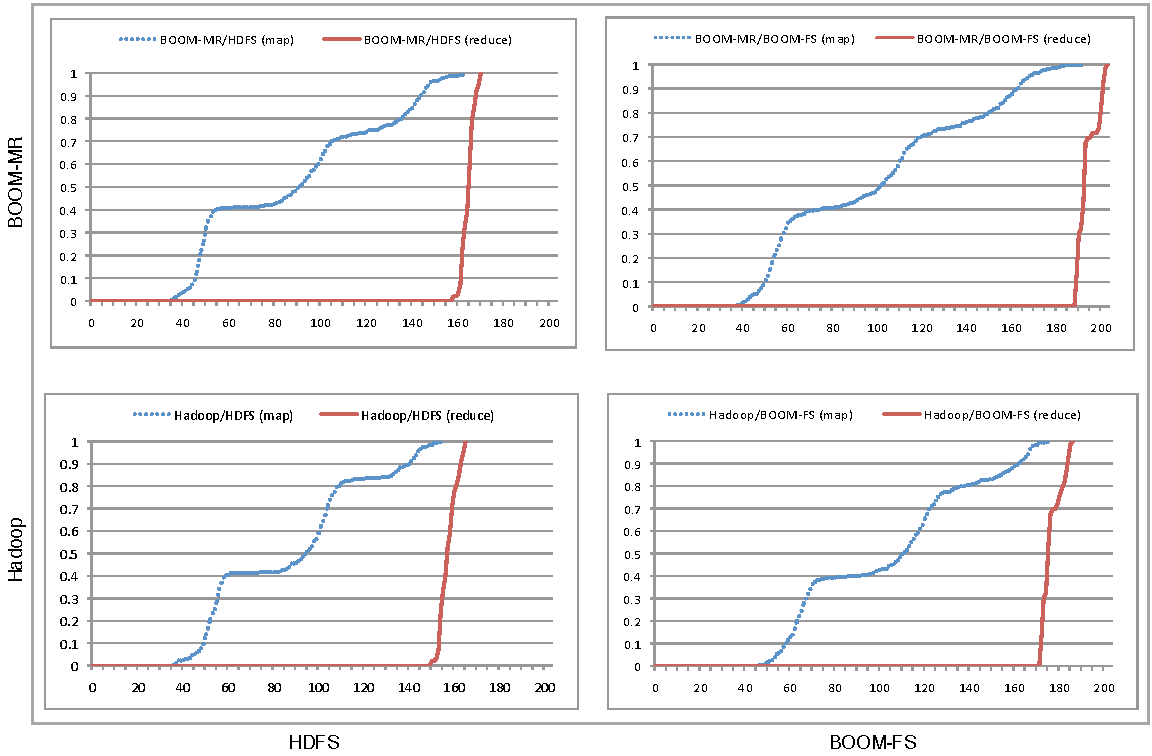
\includegraphics[scale=0.75]{figures/fourgraphs}
\caption{CDFs representing the elapsed time between job startup and task
  completion for both map and reduce tasks, for all combinations of Hadoop and \BOOM-MR
  over HDFS and \BOOM-FS\@.  In each graph, the horizontal axis is
  elapsed time in seconds, and the vertical represents the percentage of tasks completed.}
\label{fig:ec2experiment}
\end{figure*}

While improved performance was not a goal of our work, we wanted to ensure that
the performance of \BOOMA was competitive with Hadoop.  The workload was a
wordcount job on a 30 GB file, using 481 map tasks and 100 reduce tasks.

Figure~\ref{fig:ec2experiment} contains four graphs comparing the performance of
different combinations of Hadoop MapReduce, HDFS, \BOOM-MR, and \BOOM-FS\@. Each
graph reports a cumulative distribution of the elapsed time in seconds from job
startup to map or reduce task completion. The map tasks complete in three
distinct ``waves.'' This is because only 2 $\times$ 100 map tasks can be
scheduled at once. Although all 100 reduce tasks can be scheduled immediately,
no reduce task can finish until all maps have been completed because each reduce
task requires the output of all map tasks.

The lower-left graph describes the performance of Hadoop running on top of HDFS,
and hence serves as a baseline for the subsequent graphs. The upper-left graph
details \BOOM-MR running over HDFS\@. This graph shows that map and reduce task
durations under \BOOM-MR are nearly identical to Hadoop 18.2. The lower-right
and upper-right graphs detail the performance of Hadoop MapReduce and \BOOM-MR
running on top of \BOOM-FS, respectively. \BOOM-FS performance is slightly
slower than HDFS, but remains competitive.


\subsection{LATE policy}

We now compare the behavior of our LATE implementation with the results
observed by Zaharia et al.\ using Hadoop MapReduce.  LATE focuses on how to
improve job completion time by reducing the impact of ``straggler'' tasks.  To
simulate stragglers, we artificially placed additional load on six nodes.  We
ran the same wordcount job on 30 GB of data; using 481 map tasks and 400 reduce
tasks, which produced two distinct ``waves'' of reduce tasks.  We ran each
experiment five times, and report the average over these runs.

Figure~\ref{fig:ec2reduce} shows the reduce task duration CDF for three
different configurations.  The plot labeled ``No Stragglers'' represents normal
load, while the ``Stragglers'' and ``Stragglers (LATE)'' plots describe
performance in the presence in stragglers using the default FCFS policy and the
LATE policy, respectively.  We omit map task durations, because adding
artificial load had little effect on map task execution --- it just resulted in
slightly slower growth from just below 100\% to completion.

\begin{figure*}
\ssp
  \centering
  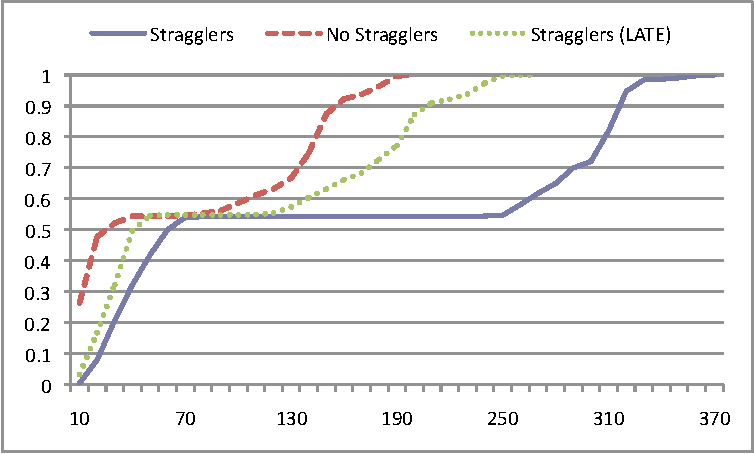
\includegraphics[scale=0.75]{figures/reduce_stragglers}
  \caption{CDF of reduce task duration (secs), with and without stragglers.}
  \label{fig:ec2reduce}
\end{figure*}

The 200 reduce tasks were scheduled concurrently with the map step.  This first
wave of reduce tasks cannot enter the reduce phase until all the map tasks have
completed, which increased their duration, and resulted in the large runtime
durations indicated in the right portion of the graph.  The second wave of 200
reduce tasks did not experience this delay due to unfinished map work since
these reduce tasks were scheduled after all map tasks had finished.  The second
wave of reduce tasks are reported in the left portion of the graph.
Consequently, stragglers had less of an impact on the second wave of reduce
tasks since fewer resources (i.e., no map work) were being consumed.
Figure~\ref{fig:ec2reduce} shows this effect, and also demonstrates how the
LATE implementation in {\BOOMA} handles stragglers much more effectively than
the default Hadoop policy.  This echoes the results reported by Zaharia et
al.~\cite{zaharia-late}

\section{Related Work}
\label{ch:boom:sec:relwork}

Declarative and data-centric languages have traditionally been considered useful
in very few domains, but things have changed substantially in recent years.
MapReduce~\cite{mapreduce-osdi} has popularized functional dataflow programming
with new audiences in computing.  Also, a surprising breadth of recent research
projects have proposed and prototyped declarative languages, including overlay
networks~\cite{p2:sosp}, three-tier web services~\cite{hilda}, natural language
processing~\cite{dyna}, modular robotics~\cite{meld}, video games~\cite{cornellgames}, 
file system metadata analysis~\cite{wiscfsck}, and compiler analysis~\cite{bddbddb}.

Most of the languages cited above are declarative in the same sense as SQL: they are 
based in first-order logic. Some --- notably MapReduce, but also SGL~\cite{cornellgames} --- are
algebraic or dataflow languages, used to describe the composition of operators that produce and 
consume sets or streams of data.  Although arguably imperative, they are far closer to logic languages 
than to traditional imperative languages like Java or C, and are often amenable to set-oriented optimization 
techniques developed for declarative languages~\cite{cornellgames}. Declarative and dataflow languages 
can also share the same runtime, as demonstrated by recent integrations of MapReduce and SQL
in Hive~\cite{hive-vldb}, DryadLINQ~\cite{DryadLINQ}, HadoopDB~\cite{hadoopdb}, and products from vendors 
such as Greenplum and Aster.

Concurrent with our work, the Erlang language was used to implement a simple MapReduce framework called 
Disco~\cite{disco} and a transactional DHT called Scalaris with Paxos support~\cite{scalaris}. Philosophically, Erlang 
revolves around concurrent {\em actors}, rather than data. A closer comparison of actor-oriented and data-centric design 
styles is beyond the scope of this dissertation, but an interesting topic for future work.

\section{Summary}
\label{ch:boom:sec:conclusion}

The initial version of \BOOM-MR required one person-month of development time
and an additional two person-months debugging and tuning \BOOM-MR's performance
for large jobs.  The final version of \BOOM-MR contained declarative
specifications for the core task scheduler (9 rules), the speculative task
scheduler (5 rules), recovery from failed tasks (3 rules), and maintenance of
various job and task related statistics (5 rules).  In total, \BOOM-MR
consisted of 22 \OVERLOG rules in 156 lines of code, and 1269 lines of Java.
\BOOM-MR was based on Hadoop version 18.2; we estimate that we removed 6,573
lines of code (out of 88,863) from the \ol{org.apache.hadoop.mapred} Hadoop
package.  In many fewer lines of code and development time, we were able to
achieve performance characteristics that were competitive to stock Hadoop.

%For this ``porting'' exercise, it was handy to leverage \JOL's Java interfaces
%and draw the Java/\OVERLOG boundaries flexibly.  This allowed us to focus on
%porting the more interesting Hadoop logic into \OVERLOG, while avoiding ports of
%relatively mechanical details.  For example, we chose to leave the data
%representation of the {\em jobConf} as a Java object rather than flatten it
%into a relation because it had no effect on the scheduling logic.

In the end, we found that scheduling policies were a good fit for a declarative
language like \OVERLOG.  In retrospect, this is because scheduling can be
decomposed into two tasks: {\em monitoring} the state of a system and applying
{\em policies} for how to react to changes to that state.  Monitoring is
well-handled by \OVERLOG: we found that the statistics about {\TT} state
required by the LATE policy are naturally realized as aggregate functions, and
\JOL took care of automatically updating those statistics as new messages from
{\TT}s arrived.  In the next chapter, we will look at importing statistics
taken from the output of a MapReduce job that is continuously monitoring
machine and process level statistics.  Once these near real-time monitoring
statistics have been imported into \JOL, we can build some very interesting
scheduling policies around them.

It is also unsurprisingly that a logic language should be well-suited to
specifying policy.  We found the \BOOM-MR scheduler much simpler to extend and
modify than the original Hadoop Java code, as demonstrated by our experience
with LATE\@.  Informally, the \OVERLOG code in \BOOM-MR seems about as complex
as it should be: Hadoop's MapReduce task coordination logic is a simple and
clean design, and the compactness of \BOOM-MR reflects that simplicity
appropriately.  The extensibility of \BOOM-MR benefited us when we extended the
MapReduce batch-oriented model to one that pipelined data between operators
(Chapter~\ref{ch:hop}); supporting both online aggregation~\cite{onlineagg} and
stream processing~\cite{stream} jobs.  
%Pipelining MapReduce required a more
%aggressive operator coscheduling policy that we captured in a few extra
%\OVERLOG rules, beyond those discussed here.


%\chapter[MapReduce Online]{MapReduce Online}
\label{ch:hop}

MapReduce is typically applied to large batch-oriented computations that do not
require any real-time completion constraints.  The Google MapReduce
framework~\cite{mapreduce-osdi} and open-source Hadoop system reinforce this
usage model through a batch-processing implementation strategy: the entire
output of each map and reduce task is {\em materialized} to a local file
before it can be consumed by the next stage.  Materialization allows for a
simple and elegant checkpoint/restart fault-tolerance mechanism that is
critical in large deployments, which have a high probability of slowdowns or
failures at worker nodes.  However, batch-processing is not a requirement for
fault-tolerance.  Moreover, batch-processing prevents many online data
processing strategies~\cite{onlineagg, borealis, stream, tcq-cidr} and its
aggressive materialization strategy can be costly in terms of efficiency e.g.,
energy~\cite{yanpei}.

In this chapter, we propose an alternative MapReduce architecture in which
intermediate data is {\em pipelined} between operators, while preserving the
programming interfaces and fault-tolerance properties of previous MapReduce
frameworks.  To validate our design, we developed the Hadoop Online Prototype
(HOP): a pipelined version of Hadoop.\footnote{The source code for HOP can be
downloaded from \url{http://code.google.com/p/hop/}}

Pipelining provides several important advantages to a MapReduce
framework, but also raises new design challenges. We highlight the
potential benefits first:
\begin{itemize}
\ssp
\item
  Since reducers begin processing data as soon as it is produced by mappers,
  they can generate and refine an approximation of their final answer during the
  course of execution. This technique, known as {\em online
    aggregation}~\cite{onlineagg}, can provide initial estimates of results
  several orders of magnitude faster than the final result.  We
  describe how we adapted online aggregation to our pipelined MapReduce
  architecture in Chapter~\ref{ch:hop:sec:online}.

\item
  Pipelining widens the domain of problems to which MapReduce can be applied. In
  Chapter~\ref{ch:hop:sec:continuous}, we show how HOP can be used to support
  {\em continuous queries}: MapReduce jobs that run continuously, accepting new
  data as it arrives and analyzing it immediately. This allows MapReduce to be
  used for applications such as event monitoring and stream processing.

\item
  Pipelining delivers data to downstream operators more promptly, which can
  increase opportunities for parallelism, improve utilization, and reduce
  response time. A thorough performance study is a topic for future work;
  however, in Chapter~\ref{ch:hop:sec:perf} we present some initial performance
  results which demonstrate that pipelining can reduce job completion times by
  up to 25\% in some scenarios.
\end{itemize}

We develop the design of HOP's pipelining scheme in
Chapter~\ref{ch:hop:sec:pipelining}, keeping the focus on traditional batch
processing tasks.  Pipelining raises several design challenges.  First,
Google's attractively simple MapReduce fault-tolerance mechanism is predicated
on the materialization of intermediate state.  In Chapter~\ref{ch:hop:sec:ft},
we show that fault-tolerance can coexist with pipelining, by allowing producers
to periodically ship data to consumers in parallel with data materialization.
A second challenge arises from the greedy communication implicit in pipelines,
which is at odds with batch-oriented optimizations supported by ``combiners'':
map-side code that reduces network utilization by performing pre-aggregation
before communication.  We discuss how the HOP design addresses this issue in
Chapter~\ref{ch:hop:sec:intra-pipe}.  Finally, pipelining requires that
producers and consumers are co-scheduled intelligently.  In
Chapter~\ref{ch:hop:sec:jolport}, we discuss some declarative scheduling
policies that try to fill the pipeline early --- by scheduling downstream
operators first --- and enforce a complete pipeline for continuous queries.

The remaining portions of this chapter focus on applications of HOP and
scheduling policies related to those applications.  In
Chapter~\ref{ch:hop:sec:online}, we show how HOP can support online aggregation
for long-running jobs and illustrate the potential benefits of that interface
to MapReduce programmers.  Chapter~\ref{ch:hop:sec:continuous} describes our
support for continuous MapReduce jobs over data streams and demonstrate an
example of a near-real-time cluster monitoring application.  In
Chapter~\ref{ch:hop:sec:boom}, we return to the topic of scheduling to address
the new challenges raised by these HOP applications.
Chapter~\ref{ch:hop:sec:jolport} describes our port of the \BOOM-MR declarative
scheduler to HOP and some new \OVERLOG scheduling policies that deal with
online aggregation and continuous jobs.  Chapter~\ref{ch:hop:sec:jolmonitor}
introduces a new speculation policy based on statistics collected by a
(continuous) MapReduce monitoring job described in
Chapter~\ref{ch:hop:sec:monitor}.  Finally, Chapter~\ref{ch:hop:sec:relwork}
concludes with some related work.

\section{Pipelined MapReduce}
\label{ch:hop:sec:pipelining}

We begin with a description of our Hadoop extensions that support pipelining
between tasks (Chapter~\ref{ch:hop:sec:intra-pipe}) and jobs
(Chapter~\ref{ch:hop:sec:inter-pipe}).  We describe how our design supports
fault-tolerance (Chapter~\ref{ch:hop:sec:ft}) and compare the performance of HOP
under both pipelining and blocking execution modes
(Chapter~\ref{ch:hop:sec:perf}).

%\begin{figure}[t]
%  \centering
%  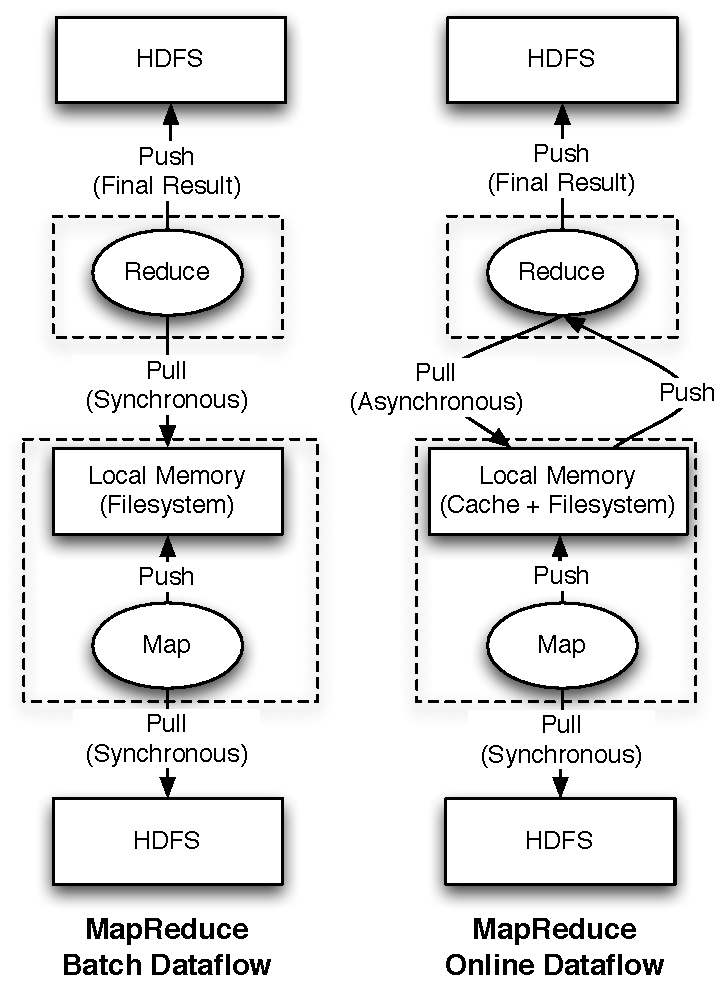
\includegraphics[width=0.90\linewidth]{figures/dataflow_arch.pdf}
%  \caption{Hadoop dataflow for batch (left) and pipelined (right) processing of MapReduce computations.}
%  \label{ch:hop:fig:pipeline}
%\end{figure}
%Figure~\ref{ch:hop:fig:pipeline} depicts the dataflow of two MapReduce
%configurations.  The dataflow on the left describes the materialization
%approach followed by stock Hadoop, while the dataflow on the right allows
%pipelining.  In the remainder of this section, we present our design and
%implementation for the pipelined Hadoop dataflow.  We describe how our design
%supports fault tolerance (Section~\ref{ch:hop:sec:ft}), and discuss the
%interaction between pipelining and task scheduling
%(Section~\ref{ch:hop:sec:pipeline-sched}).

\subsection{Pipelining Within A Job}
\label{ch:hop:sec:intra-pipe}

As described in Chapter~\ref{ch:hadoop:sec:reducetask}, reduce tasks
traditionally issue HTTP requests to {\em pull} their input from each {\TT}
that hosted a map task belonging to the same job.  A \TT is responsible for
serving these HTTP requests, which could occur long after the map task's
execution.  This means that map task execution is completely decoupled from
reduce task execution.  To support pipelining, we modified the \TT serving
component to {\em push} data to reducers as it is produced by the map tasks,
while still maintaining the decoupling of these two steps.  To give an
intuition for how this works, we begin by describing a straightforward
pipelining design, and then discuss the changes we had to make to achieve good
performance.

\subsubsection{Na\"{\i}ve Pipelining}
\label{ch:hop:sec:naive}

We begin with a na\"{\i}ve implementation that sends data directly from map to
reduce tasks via a TCP socket.  Immediately, this design couples the execution
of map and reduce task executions, forcing us to schedule {\em all} reduce
tasks before any one map task.  Consequently, this design does not scale, most
notably when there is not sufficient reduce task slot capacity, but there are
other ramifications that we discuss here before converging on the true HOP
design.

Recall, that when a client submits a new job to Hadoop, the {\JT} assigns the
map and reduce tasks associated with the job to the available {\TT} slots.  For
purposes of {\em this} discussion, we must assume that there are enough free
slots to assign all reduce tasks in a job.  We modified Hadoop so that each
reduce task contacts every map task upon initiation of the job, and opens a TCP
socket which will be used to pipeline the output of the map function.  As each
map output record is produced, the mapper determines which partition (reduce
task) the record should be sent to, and immediately sends it via the
appropriate socket.

A reduce task accepts the pipelined data it receives from each map task and
stores it in an in-memory buffer, spilling sorted runs of the buffer to disk as
needed. Once the reduce task learns that every map task has completed, it
performs a final merge of all the sorted runs and applies the user-defined
reduce function as normal.

\subsubsection{Refinements}
\label{ch:hop:sec:pipe-refine}

While the algorithm described above is straightforward, it suffers from several
practical problems.  First, it is possible that there will not be enough slots
available to schedule every task in a new job.  Opening a socket between every
map and reduce task also requires a large number of TCP connections.  A simple
tweak to the na\"{\i}ve design solves both problems: if a reduce task has not
yet been scheduled, any map tasks that produce records for that partition
simply write them to disk.  When the map task completes, it registers the output
it was not able to send with the host \TT serving component.  Once the reduce
task is assigned a slot, it can then pull the records from the map task's host
\TT, as in regular Hadoop.  To reduce the number of concurrent TCP connections,
each reducer can be configured to pipeline data from a bounded number of
mappers at once; the reducer will pull data from the remaining map tasks in the
traditional Hadoop manner.

Our initial pipelining implementation suffered from a second problem: the map
function was invoked by the same thread that wrote output records to the
pipeline sockets.  This meant that if a network I/O operation blocked (e.g.,
because the reducer was over-utilized), the mapper was prevented from doing
useful work.  Pipeline stalls should not prevent a map task from making
progress -- especially since, once a task has completed, it frees a {\TT} slot
to be used for other purposes.  We solved this problem by running the map
function in a separate thread that stores its output in an in-memory buffer,
and then having another thread periodically send the contents of the buffer to
the connected reducers.~\footnote{This code was based on the existing Hadoop
SpillThread component, which is responsible for writing map output to disk
concurrently with the ``map function.''}

\subsubsection{Granularity of Map Output}
\label{ch:hop:sec:mapout}

Another problem with the na\"{\i}ve design is that it eagerly sends each record
as soon as it is produced, which prevents the use of map-side combiners.
Imagine a job where the reduce key has few distinct values (e.g., gender), and
the reduce applies an algebraic aggregate function (e.g., count).  As discussed
in Chapter~\ref{ch:hadoop:sec:progmodel}, combiners allow map-side
``pre-aggregation'': by applying a reduce-like function to each distinct key at
the mapper, network traffic can often be substantially reduced.  Eagerly
pipelining each record as it is produced prevents the use of these map-side
combiners.

Another related problem is that eager pipelining moves some of the sorting work
from the mapper to the reducer.  Recall from
Chapter~\ref{ch:hadoop:sec:maptask}, that in the blocking architecture, map
tasks generate sorted spill files: all the reduce task must do is merge
together the pre-sorted map output for each partition.  In the na\"{\i}ve
pipelining design, map tasks send output records as they are generated, so a
reducer (scheduled early) must perform a full external sort.  Because the
number of map tasks typically far exceeds the number of
reduces~\cite{mapreduce-osdi}, moving more work to the reducer increased
response time, as shown in our experiments (Chapter~\ref{ch:hop:sec:perf}).

To avoid a heavy reduce task sort, instead of sending the buffer contents to
reducers directly, we wait for the buffer to grow to a threshold size.  The
mapper then (quick) sorts the output by partition and reduce key, applies the
combiner function, and writes the buffer to disk using the Hadoop spill file
format described in Figure~\ref{ch:hadoop:fig:mapoutput}.  Next, we arranged
for the {\TT} serving component at each node to handle pipelining data to
reduce tasks.  Map tasks register spill files with the {\TT} via
RPCs.~\footnote{We extended the existing RPC Hadoop interface to include
information on individual spill files.  Having the spill files be in the same
format allowed us to reuse much of the stock Hadoop serving code i.e., I/O file
formats/streams.}  If the reducers are able to keep up with the production of
map outputs and the network is not a bottleneck, a spill file will be sent to a
reducer soon after it has been produced (in which case, the spill file is
likely still resident in the map machine's kernel buffer cache).  However, if a
reducer begins to fall behind, the number of unsent spill files will grow.

When a map task generates a new spill file, it first queries the {\TT} for the
number of unsent spill files.  If this number grows beyond a certain threshold
(two unsent spill files in our experiments), the map task does not immediately
register the new spill file with the {\TT}.  Instead, the mapper will
accumulate multiple spill files.  Once the queue of unsent spill files falls
below the threshold, the map task merges and combines the accumulated spill
files into a single file, and then resumes registering its output with the
{\TT}.  This simple flow control mechanism has the effect of {\em adaptively}
moving load from the reducer to the mapper or vice versa, depending on which
node is the current bottleneck.

A similar mechanism is also used to control how aggressively the combiner
function is applied.  The map task records the ratio between the input and
output data sizes whenever it invokes the combiner function.  If the combiner
is effective at reducing data volumes, the map task accumulates more spill
files (and applies the combiner function to all of them) before registering
that output with the {\TT} for pipelining.\footnote{Our current prototype uses
a simple heuristic: if the combiner reduces data volume by $\frac{1}{k}$ on
average, we wait until $k$ spill files have accumulated before registering them
with the {\TT}.  A better heuristic would also account for the computational
cost of applying the combiner function.}

The connection between pipelining and adaptive query processing techniques has
been observed elsewhere (e.g.,~\cite{eddies, bamboo}).  The adaptive scheme
outlined above is relatively simple, but we believe that adapting to feedback
along pipelines has the potential to significantly improve the utilization of
MapReduce clusters.

\subsection{Pipelining Between Jobs}
\label{ch:hop:sec:inter-pipe}

Many practical computations cannot be expressed as a single MapReduce job, and
the outputs of higher-level languages like Pig~\cite{pig-sigmod} typically involve
multiple jobs.  In the traditional Hadoop architecture, the output of each job
is written to HDFS in the reduce step and then immediately read back from HDFS
by the map step of the next job. Furthermore, the {\JT} cannot schedule a
consumer job until the producer job has completed, because scheduling a map task
requires knowing the HDFS block locations of the map's input split.

In our modified version of Hadoop, the reduce tasks of one job can optionally
pipeline their output directly to the map tasks of the next job, sidestepping
the need for expensive fault-tolerant storage in HDFS for what amounts to a
temporary file.  Unfortunately, the computation of the reduce function from the
previous job and the map function of the next job cannot be overlapped: the
final result of the reduce step cannot be produced until all map tasks have
completed, which prevents effective pipelining.  However, we describe later how
online aggregation and continuous query pipelines can publish ``snapshot''
outputs that can indeed pipeline between jobs.

\subsection{Fault Tolerance}
\label{ch:hop:sec:ft}

% nrc: (1) Quantify the overhead added by tracking map task origin (2)
% Did we implement the "don't rerun map task from scratch" idea?

Our pipelined Hadoop implementation is robust to the failure of both
map and reduce tasks. To recover from map task failures, we added
bookkeeping to the reduce task to record which map task produced each
pipelined spill file. To simplify fault-tolerance, the reducer treats
the output of a pipelined map task as ``tentative'' until the {\JT}
informs the reducer that the map task has committed successfully. The
reducer can merge together spill files generated by the same
uncommitted mapper, but will not combine those spill files with the
output of other map tasks until it has been notified that the map task
has committed. Thus, if a map task fails, each reduce task can ignore
any tentative spill files produced by the failed map attempt. The
{\JT} will take care of scheduling a new map task attempt, as in stock
Hadoop. 

If a reduce task fails and a new copy of the task is started, the new
reduce instance must be sent all the input data that was sent to the
failed reduce attempt. If map tasks operated in a purely pipelined
fashion and discarded their output after sending it to a reducer, this
would be difficult. Therefore, map tasks retain their output data on
the local disk for the complete job duration. This allows the map's output to be 
reproduced if any reduce tasks fail. For batch jobs, the key advantage of our architecture is
that reducers are not blocked waiting for the complete output of the
task to be written to disk.

Our technique for recovering from map task failure is straightforward, but
places a minor limit on the reducer's ability to merge spill files. To avoid
this, we envision introducing a ``checkpoint'' concept: as a map task runs, it
will periodically notify the {\JT} that it has reached offset $x$ in its input
split. The {\JT} will notify any connected reducers; map task output that was
produced before offset $x$ can then be merged by reducers with other map task
output as normal. To avoid duplicate results, if the map task fails, the new map
task attempt resumes reading its input at offset $x$. This technique would also
reduce the amount of redundant work done after a map task failure or during
speculative execution of ``backup'' tasks~\cite{mapreduce-osdi}.

\subsection{Performance Evaluation}
\label{ch:hop:sec:perf}

A thorough performance comparison between pipelining and blocking is not the
focus of this work.  However, as future work we plan to investigate a
rule-based (e.g., Evita Raced) optimizer for Hadoop MapReduce that considers
pipelined plans in its search strategy.  Here, we demonstrate that pipelining
can reduce job completion times in some configurations and should be considered
by any such optimizer.

We report performance using both large (512MB) and small (32MB) HDFS block
sizes using a single workload (a wordcount job over randomly-generated text).
Since the words were generated using a uniform distribution, map-side combiners
were ineffective for this workload.  We performed all experiments using
relatively small clusters of Amazon EC2 nodes.  We also did not consider
performance in an environment where multiple concurrent jobs are executing
simultaneously.

\subsubsection{Background and Configuration}

Before diving into the performance experiments, it is important to further
describe the division of labor in a HOP job, which is broken into task phases.
A map task consists of two work phases: {\em map} and {\em sort}.  Much of the
work performed during the job happens in the {\em map} phase, where the map
function is applied to each record in the input and subsequently sent to an
output buffer.  Once the entire input has been processed, the map task enters
the {\em sort} phase, where a final merge sort of all intermediate spill files
is performed before registering the final output with the \TT.  The progress
reported by a map task corresponds to the {\em map} phase, which is overlapped
with many in-memory record buffer sorts and subsequent spills to local files.

A reduce task in HOP is divided into three work phases: {\em shuffle}, {\em
reduce}, and {\em commit}.  In the {\em shuffle} phase, reduce tasks receive
their portion of the output from each map.  In HOP, the {\em shuffle} phase
consumes 75\% of the overall reduce task progress while the remaining 25\% is
allocated to the {\em reduce} and {\em commit} phase.~\footnote{The stock
version of Hadoop divides the reduce progress evenly among the three phases.
We deviated from this approach because we wanted to focus more on the progress
during the {\em shuffle} phase.} In the {\em shuffle} phase, reduce tasks
periodically perform a merge sort on the already received map output.  These
intermediate merge sorts decrease the amount of sorting work performed at the
end of the {\em shuffle} phase.  After receiving its portion of data from all
map tasks, the reduce task performs a final merge sort and enters the {\em
reduce} phase.

By pushing work from map tasks to reduce tasks more aggressively, pipelining
can enable better overlapping of map and reduce computation, especially when
the node on which a reduce task is scheduled would otherwise be underutilized.
However, when reduce tasks are already the bottleneck, pipelining offers fewer
performance benefits, and may even hurt performance by placing additional load
on the reduce nodes.

The {\em sort} phase in the map task minimizes the merging work that reduce
tasks must perform at the end of the {\em shuffle} phase.  When pipelining is
enabled, the {\em sort} phase is avoided since map tasks have already sent some
fraction of the spill files to concurrently running reduce tasks.  Therefore,
pipelining increases the merging workload placed on the reducer.  The adaptive
pipelining scheme described in Chapter~\ref{ch:hop:sec:mapout} attempts to
ensure that reduce tasks are not overwhelmed with additional load.

We used two Amazon EC2 clusters depending on the size of the experiment:
``small'' jobs used 10 worker nodes, while ``large'' jobs used 20.  Each node
was an ``extra large'' EC2 instances with 15GB of memory and four virtual
cores, each running at 2.4GHz with a 2GB L2 cache.

\subsubsection{Small Job Results}

\begin{figure*}[t]
\ssp
\begin{minipage}{0.5\linewidth}
  \centering
        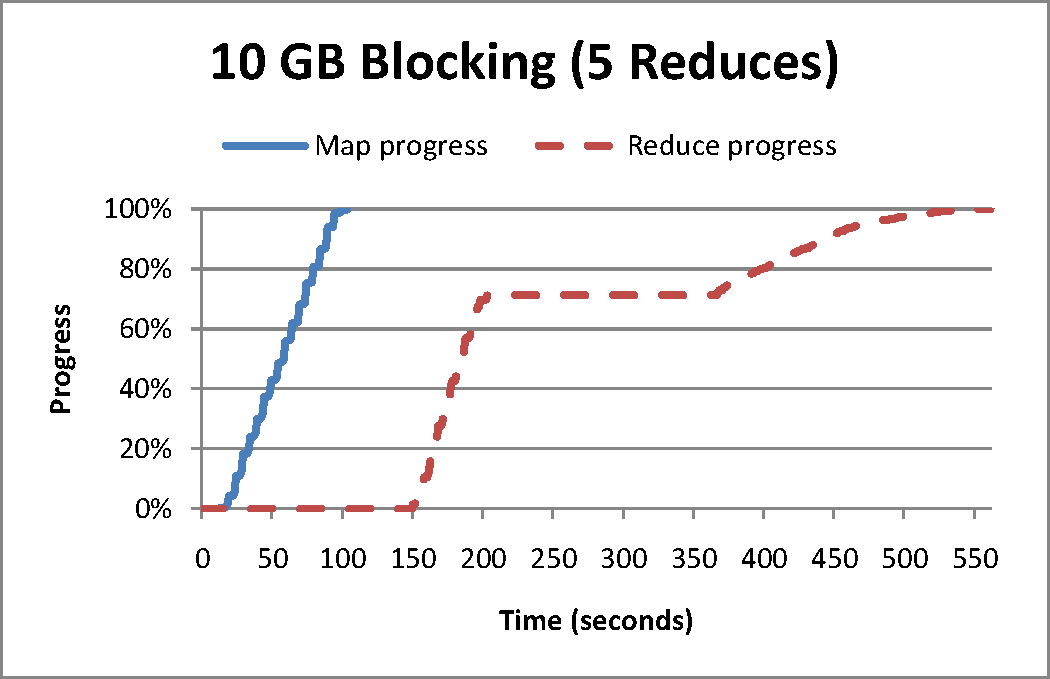
\includegraphics[width=0.90\linewidth]{figures/wc_10gb_20m5r_blocking}
\end{minipage}
\begin{minipage}{0.5\linewidth}
  \centering
        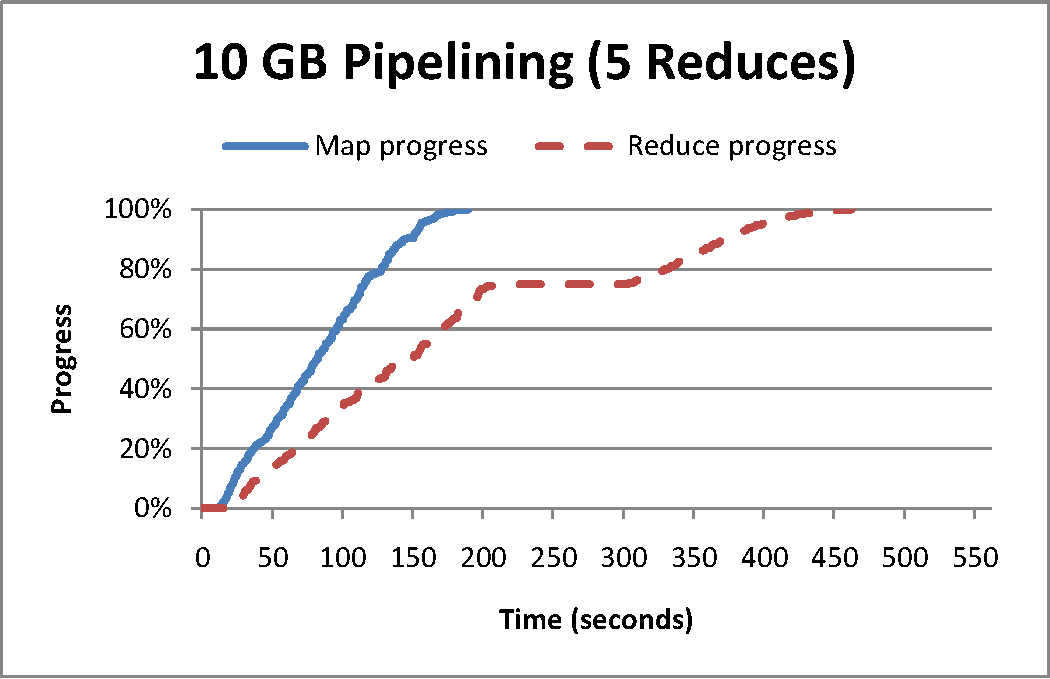
\includegraphics[width=0.90\linewidth]{figures/wc_10gb_20m5r_pipeline}
\end{minipage}
\caption{CDF of map and reduce task completion times for a 10GB wordcount job
  using 20 map tasks and 5 reduce tasks (512MB block size). The total job
  runtimes were 561 seconds for blocking and 462 seconds for pipelining.}
\label{ch:hop:fig:wc1}
\end{figure*}

\begin{figure*}[t]
\ssp
\begin{minipage}{0.5\linewidth}
  \centering
        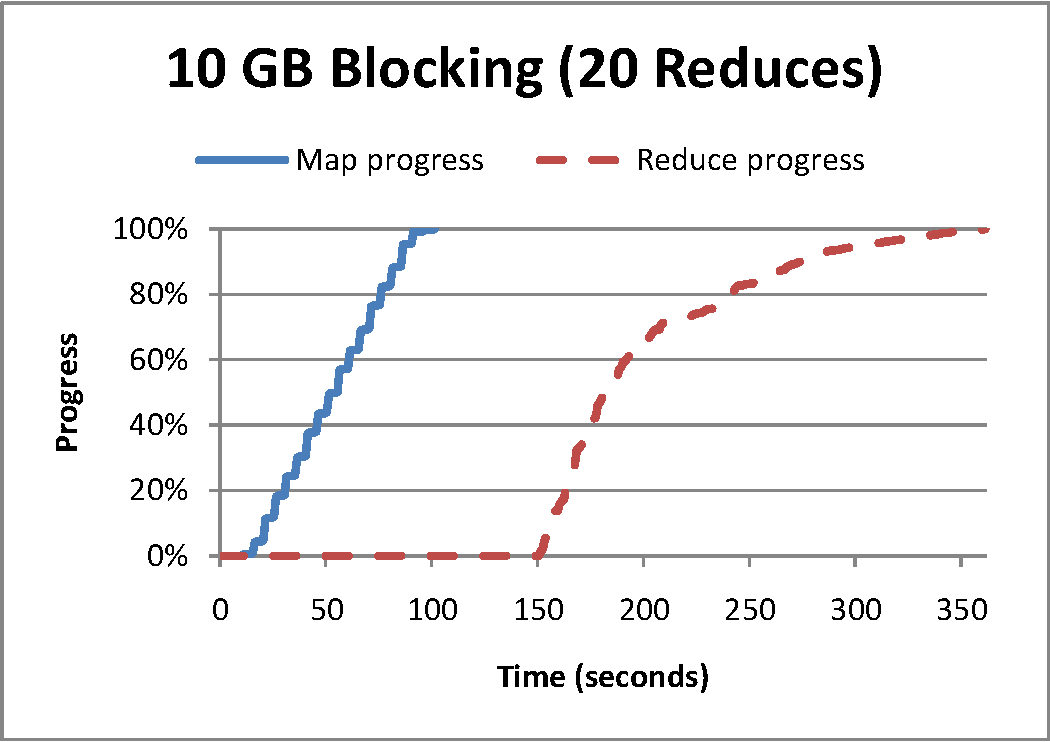
\includegraphics[width=0.88\linewidth]{figures/wc_10gb_20m20r_blocking}
\end{minipage}
\begin{minipage}{0.5\linewidth}
  \centering
        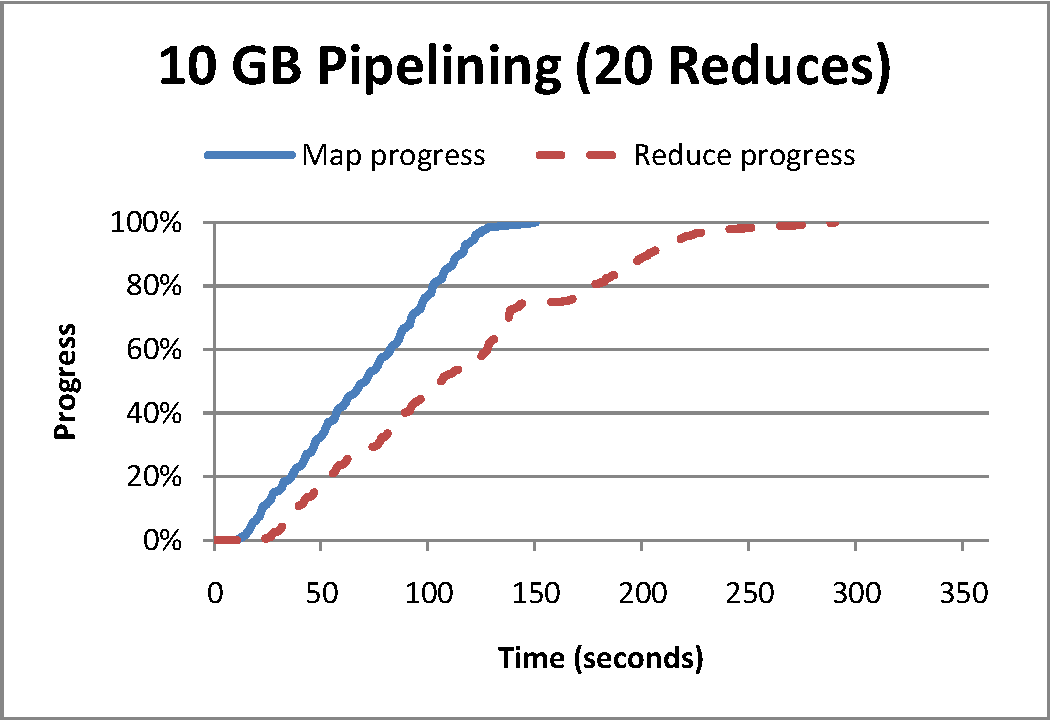
\includegraphics[width=0.90\linewidth]{figures/wc_10gb_20m20r_pipeline}
\end{minipage}
\caption{CDF of map and reduce task completion times for a 10GB wordcount job
  using 20 map tasks and 20 reduce tasks (512MB block size). The total job
  runtimes were 361 seconds for blocking and 290 seconds for pipelining.}
\label{ch:hop:fig:wc2}
\end{figure*}

\begin{figure*}[t]
\ssp
\begin{minipage}{0.5\linewidth}
  \centering
        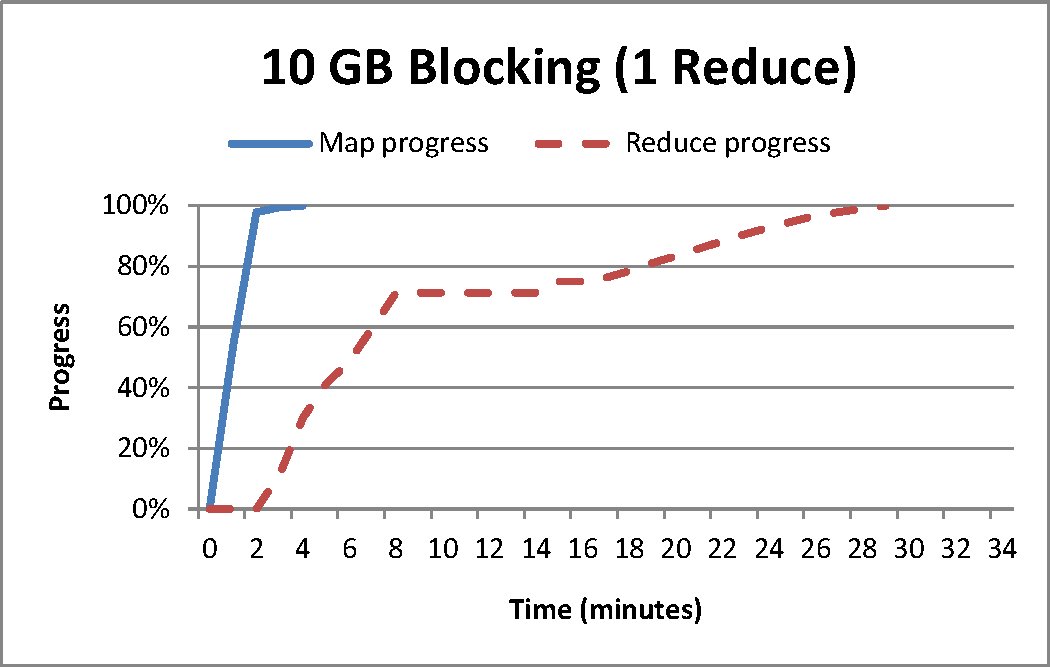
\includegraphics[width=0.95\linewidth]{figures/wc_10gb_20m1r_blocking}
\end{minipage}
\begin{minipage}{0.5\linewidth}
  \centering
        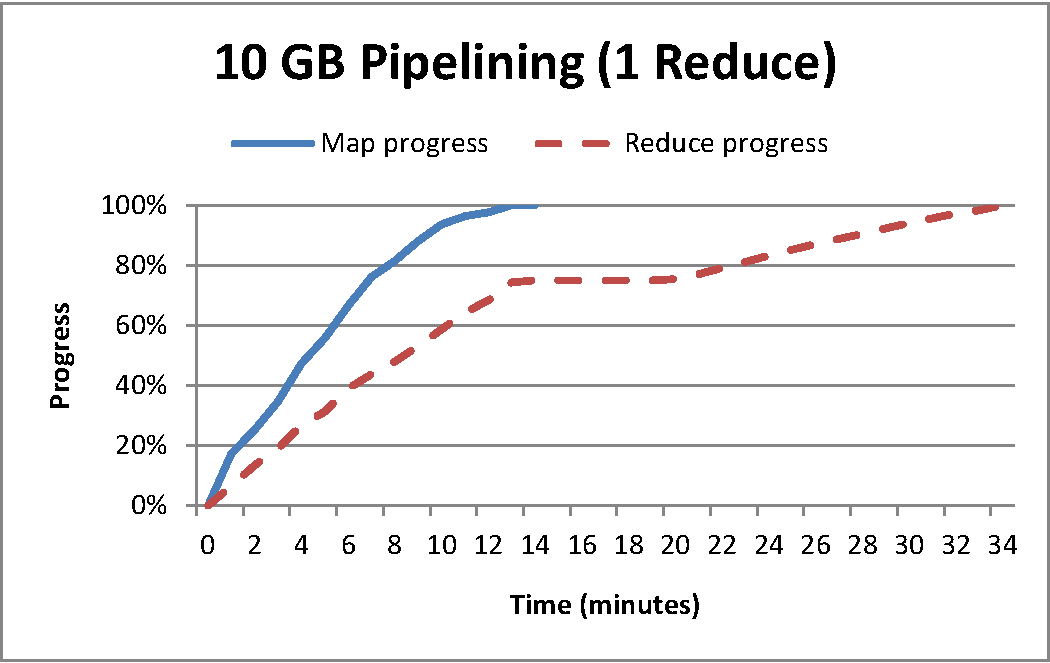
\includegraphics[width=0.95\linewidth]{figures/wc_10gb_20m1r_pipeline}
\end{minipage}
\caption{CDF of map and reduce task completion times for a 10GB wordcount job
  using 20 map tasks and 1 reduce task (512MB block size). The total job
  runtimes were 29 minutes for blocking and 34 minutes for pipelining.}
\label{ch:hop:fig:wc3}
\end{figure*}


Our first experiment focused on the performance of small jobs in an
underutilized cluster.  We ran a 10GB wordcount with a 512MB block size,
yielding 20 map tasks (one per block).  We used 10 worker nodes and configured
each worker to execute at most two map and two reduce tasks simultaneously.  We
ran several experiments to compare the performance of blocking and pipelining
using different numbers of reduce tasks.  For each experiment, we report the
average progress over five separate runs. 

Figure~\ref{ch:hop:fig:wc1} reports the results of a job configured with five
reduce tasks.  A plateau can be seen at 75\% progress for both blocking and
pipelining.  At this point in the job, all reduce tasks have completed the {\em
shuffle} phase; the plateau is caused by the time taken to perform a final
merge of all map output before entering the {\em reduce} phase.  Notice that
the plateau for the pipelining case is shorter.  With pipelining, reduce tasks
receive map outputs much earlier and can begin sorting earlier, thereby
reducing the time required for the final merge.

Figure~\ref{ch:hop:fig:wc2} reports the results with twenty reduce tasks.
Using more reduce tasks decreases the amount of merging that any one reduce
task must perform, which reduces the duration of the plateau at 75\% progress.
In the blocking case, the plateau is practically gone.  However, with
pipelining we still see a small plateau at 75\% that, through further analysis
using \ol{iostat}, can be attributed to extra disk I/Os in the pipelining case.
This extra memory pressure is due to diminished effectiveness of the combiner
in the pipelining case.  Although the response time of pipelining job is better
than the blocking, a job that contains a more effective combiner may be better
executed in blocking mode.

We further note that in both experiments, the map phase finishes faster with
blocking than with pipelining.  This is because pipelining allows reduce tasks
to begin executing earlier and perform more work (sorting and combining);
hence, the reduce tasks compete for resources with the map tasks, causing the
map phase to take slightly longer.  In this case, the increase in map duration
is outweighed by the increase in cluster utilization, resulting in shorter job
completion times: pipelining reduced completion time by 17.7\% with 5 reducers
and by 19.7\% with 20 reducers.

Figure~\ref{ch:hop:fig:wc3} describes an experiment in which we ran a 10GB
wordcount job using a single reduce task.  This caused job completion times to
increase dramatically for both pipelining and blocking, because of the extreme
load placed on the reduce node.  Pipelining delayed job completion by about
17\%, which suggests that our simple adaptive flow control scheme
(Chapter~\ref{ch:hop:sec:mapout}) was unable to move load back to the map tasks
aggressively enough in this (extremely) unbalanced job configuration.

\subsubsection{Large Job Results}

\begin{figure*}[t]
\ssp
\begin{minipage}{0.5\linewidth}
  \centering
        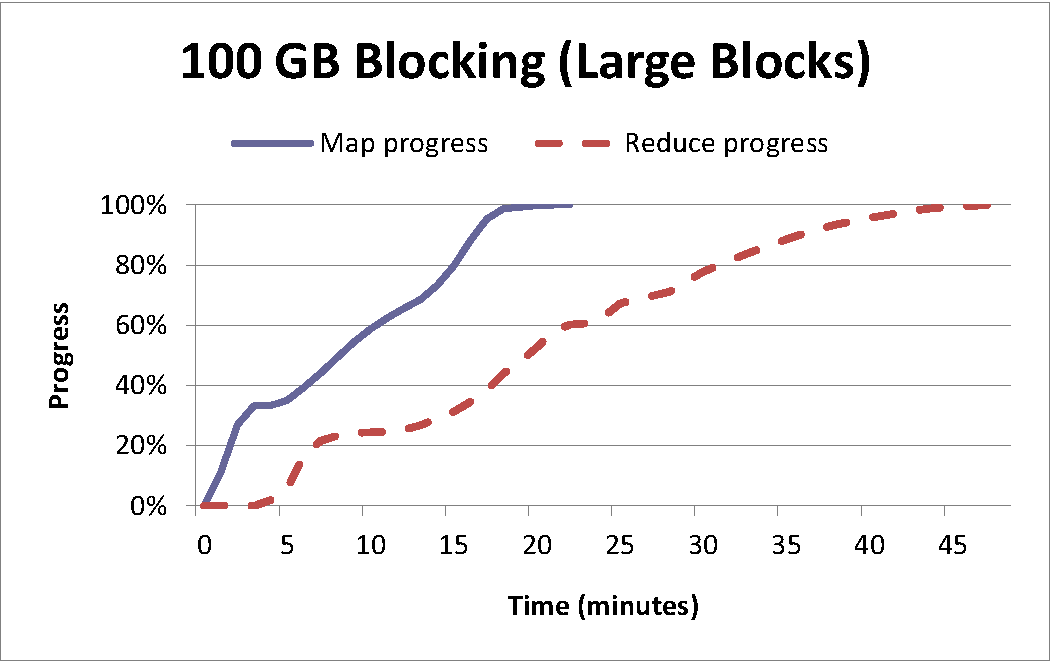
\includegraphics[width=0.95\linewidth]{figures/wc_100gb_240m60r_blocking}
\end{minipage}
\begin{minipage}{0.5\linewidth}
  \centering
        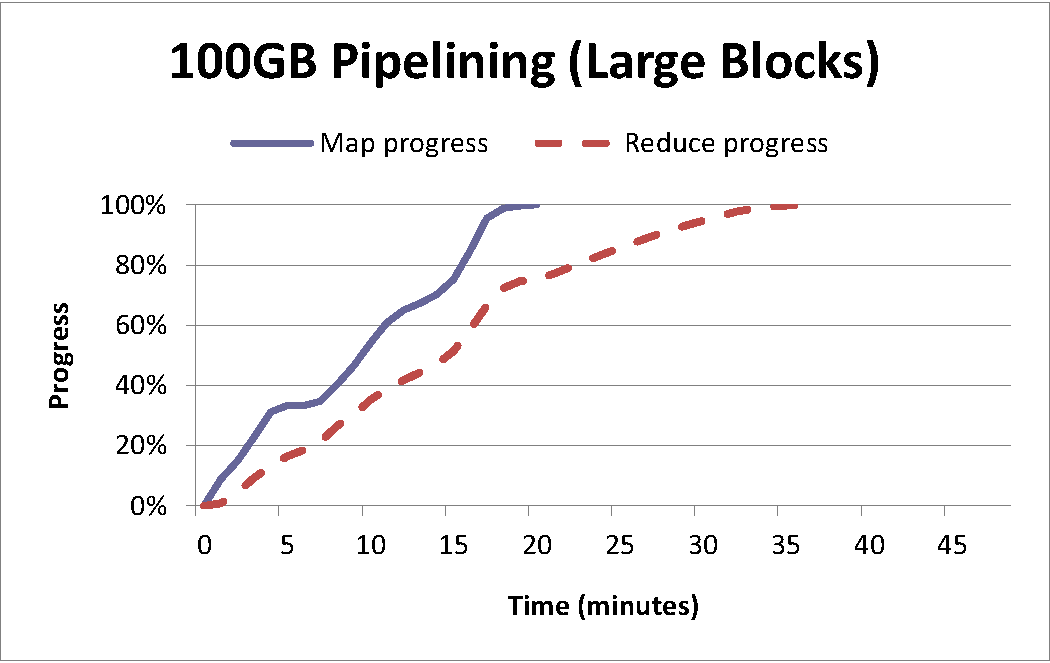
\includegraphics[width=0.95\linewidth]{figures/wc_100gb_240m60r_pipeline}
\end{minipage}
\caption{CDF of map and reduce task completion times for a 100GB wordcount job
  using 240 map tasks and 60 reduce tasks (512MB block size). The total job
  runtimes were 48 minutes for blocking and 36 minutes for pipelining.}
\label{ch:hop:fig:wc4}
\end{figure*}

\begin{figure*}[t]
\ssp
\begin{minipage}{0.5\linewidth}
  \centering
        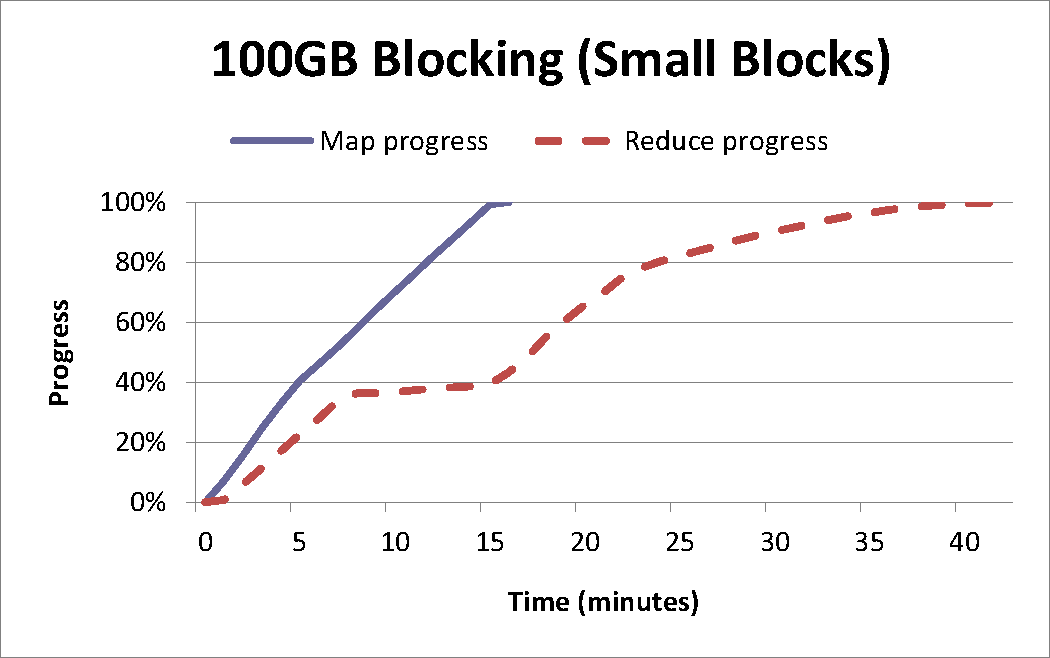
\includegraphics[width=0.95\linewidth]{figures/wc_100gb_3120m60r_blocking}
\end{minipage}
\begin{minipage}{0.5\linewidth}
  \centering
        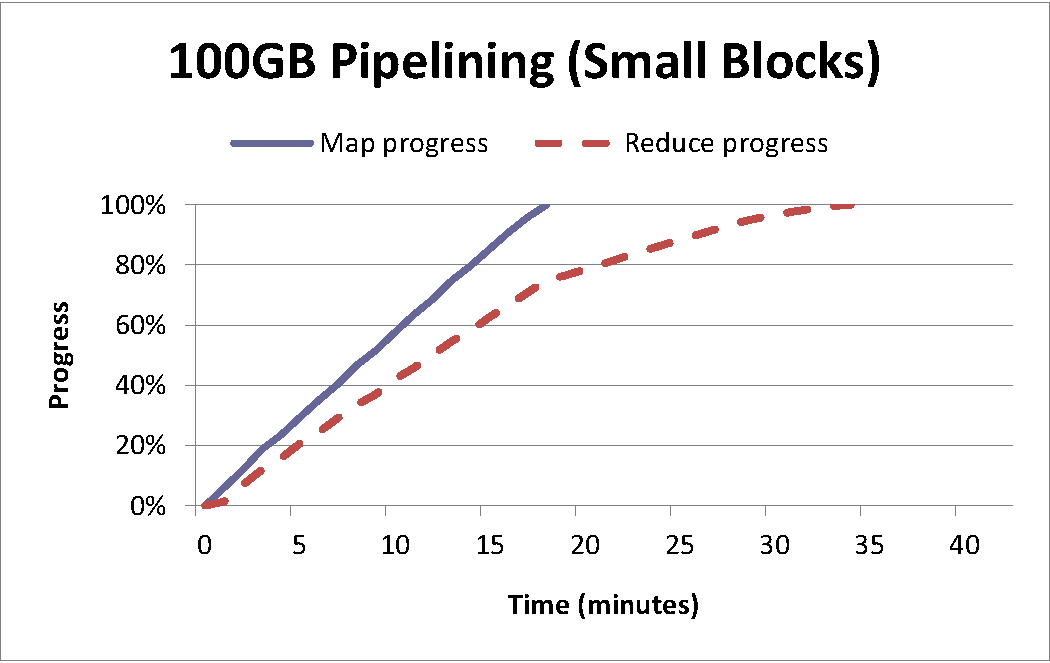
\includegraphics[width=0.95\linewidth]{figures/wc_100gb_3120m60r_pipeline}
\end{minipage}
\caption{CDF of map and reduce task completion times for a 100GB wordcount job
  using 3120 map tasks and 60 reduce tasks (32MB block size). The total job
  runtimes were 42 minutes for blocking and 34 minutes for pipelining.}
\label{ch:hop:fig:wc5}
\end{figure*}

Our second set of experiments focused on the performance of somewhat larger
jobs. We increased the input size to 100GB (from 10GB) and the number of worker
nodes to 20 (from 10). Each worker was configured to execute at most four map
and three reduce tasks, which meant that at most 80 map and 60 reduce tasks
could execute at once. We conducted two sets of experimental runs, each run
comparing blocking to pipelining using either large (512MB) or small (32MB)
block sizes. We were interested in blocking performance with small block sizes
because blocking can effectively emulate pipelining if the block size is small
enough.

Figure~\ref{ch:hop:fig:wc4} reports the performance of a 100GB wordcount job
with 512MB blocks, which resulted in 240 map tasks, scheduled in three waves of
80 tasks each.  The 60 reduce tasks were co-scheduled with the first wave of map
tasks.  In the blocking case, the reduce tasks began working as soon as they
received the output of the first wave, which is why the reduce progress begins
to climb around four minutes (well before the completion of all maps).
Pipelining was able to achieve significantly better cluster utilization, and
hence reduced job completion time by about 25\%.

Comparing the reduce progress in blocking to pipelining, we see that reduce
tasks make more progress during the {\em shuffle} phase when pipelining is
enabled. What is even more interesting is that the {\em reduce} phase is also
shorter in the case of pipelining. The reason for this is subtle; all reduce
tasks enter the {\em phase} around the same time since data is shipped in
smaller increments. In the blocking case, when the final wave of map tasks
finish they all try to send the entire output to reduce tasks at the same time,
which increases the variance on receiving the complete output from all map
tasks. That is, some reduce tasks enter the {\em reduce} phase well in advance
of others.

Figure~\ref{ch:hop:fig:wc5} reports the performance of blocking and pipelining
using 32MB blocks.  While the performance of pipelining remained similar, the
performance of blocking improved considerably, but still trailed somewhat
behind pipelining.  Using block sizes smaller than 32MB did not yield a
significant performance improvement in our experiments.

% \subsection{Discussion}

% As mentioned before, a complete performance evaluation is beyond the scope
% for this paper and we leave such a study for future work.  The focus here was
% to provide some initial insight into the performance benefits of pipelining.
% We also wanted to evaluate the adaptive policy of our pipelining scheme.  To
% this end, we found such a policy paramount in discovering the right amount of
% pipelining to perform based on runtime factors; network capacity and reduce
% task (consumer) load.

%\begin{figure*}[t]
%\begin{minipage}{0.5\linewidth}
%        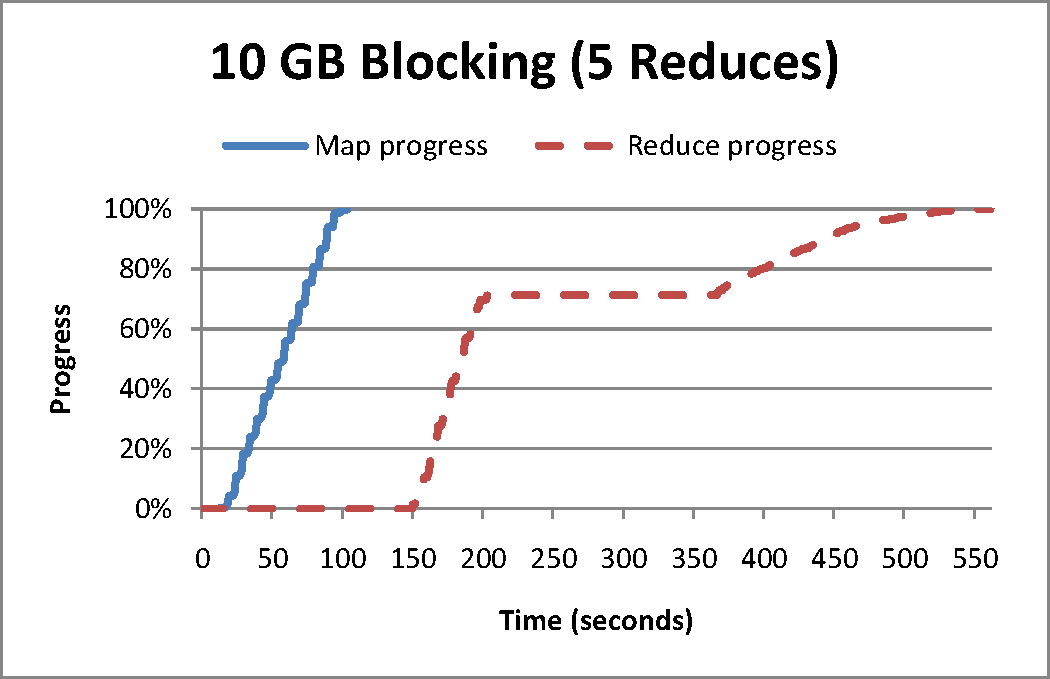
\includegraphics[width=0.95\linewidth]{figures/wc_10gb_20m5r_blocking}
%\end{minipage}
%\begin{minipage}{0.5\linewidth}
%        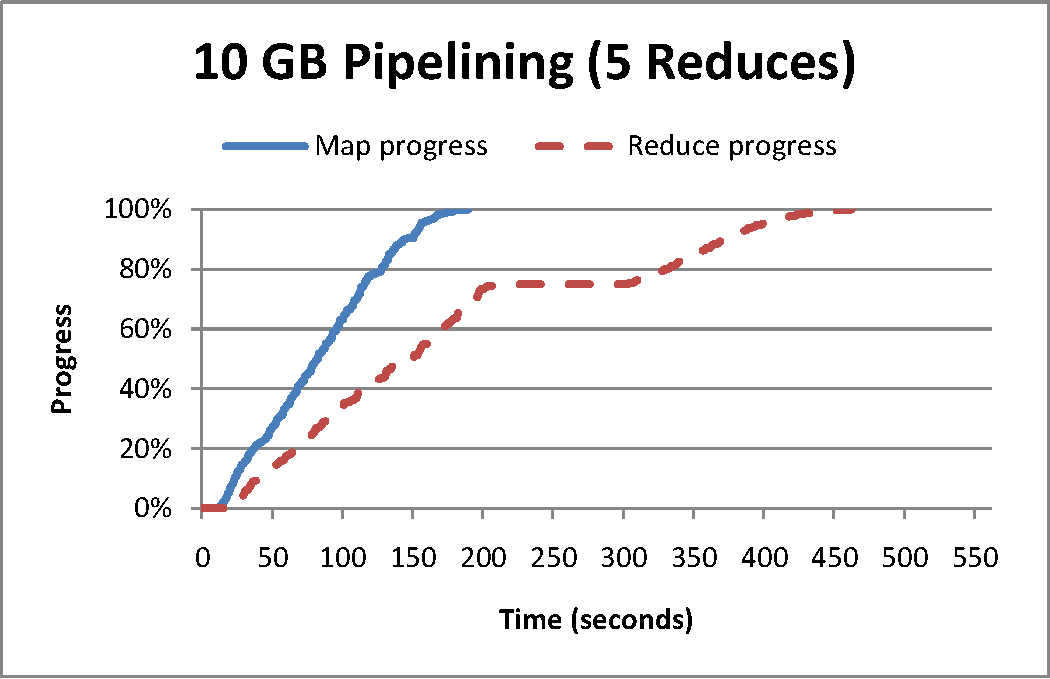
\includegraphics[width=0.95\linewidth]{figures/wc_10gb_20m5r_pipeline}
%\end{minipage}
%\caption{CDF of map and reduce task completion times for a sort job on
%  5.5GB of text extracted from Wikipedia. The total job runtimes were
%  927 seconds for blocking, and 610 seconds for pipelining.}
%\label{fig:sort}
%\end{figure*}

%We conducted a series of performance experiments using a 60-node
%cluster on Amazon EC2. One node executed the Hadoop \JT\ and the HDFS
%\NN, while the remaining 59 nodes served as slaves for running the
%{\TT}s and HDFS {\DN}s. All nodes executed on ``high-CPU medium'' EC2
%instances with 1.7GB of memory and two virtual cores. Each virtual
%core is the equivalent of a 2007-era 2.5Ghz Intel Xeon processor.

%We began by measuring the performance of a simple MapReduce job that
%does not use a combiner. Sorting is commonly used as a benchmark for
%basic MapReduce performance, because of the implicit sort done by the
%reduce phase. We sorted 5.5GB of article text extracted from
%Wikipedia; each word from the text was parsed as a separate
%record. Figure~\ref{fig:sort} describes sort performance on the EC2
%cluster using an HDFS block size of 128MB (yielding 40 map tasks). We
%configured the system to use 59 reducers. In each graph, we give the
%CDF of map and reduce task completion. The left and right graphs
%depict blocking and pipelined performance, respectively.

%Pipelining dominates blocking for this configuration, in part because
%it achieves better cluster utilization: the reduce tasks in the
%blocking job were idle for the first $192$ seconds of the experiment,
%whereas for the pipelined job, reducers began doing useful work within
%$20$ seconds. Note that in a highly-utilized cluster, increased
%pipeline parallelism would not necessarily lead to an improvement in
%total throughput. However, these results suggest that pipelining can
%substantially reduce the response time of an individual job, which can
%often be important (e.g., quickly executing high-priority jobs).


\section{Online Aggregation}
\label{ch:hop:sec:online}

Although MapReduce was originally designed as a batch-oriented system,
it is often used for interactive data analysis: a user submits a job
to extract information from a data set, and then waits to view the
results before proceeding with the next step in the data analysis
process. This trend has accelerated with the development of high-level
query languages that are executed as MapReduce jobs, such as
Hive~\cite{hive-vldb}, Jaql~\cite{jaql}, Pig~\cite{pig-sigmod}, and Sawzall~\cite{sawzall}.

Traditional MapReduce implementations provide a poor interface for interactive
data analysis, because they do not emit any output until the job has been
executed to completion.  In many cases, an interactive user would prefer a
``quick and dirty'' approximation over a correct answer that takes much longer
to compute.  In the database literature, online aggregation has been proposed
to address this problem~\cite{onlineagg}, but the batch-oriented nature of
traditional MapReduce implementations makes these techniques difficult to
apply.  Here, we show how we extended our pipelined Hadoop implementation to
support online aggregation within a single job
(Chapter~\ref{ch:hop:sec:online-single}) and between multiple jobs
(Chapter~\ref{ch:hop:sec:online-multi}).  In
Chapter~\ref{ch:hop:sec:online-eval}, we evaluate online aggregation on two
different data sets, and show that it can yield an accurate approximate answer
long before the job has finished executing.

\subsection{Single-Job Online Aggregation}
\label{ch:hop:sec:online-single}

In HOP, the data records produced by map tasks are sent to reduce tasks shortly
after each record is generated. However, to produce the final output of the job,
the reduce function cannot be invoked until the entire output of every map task
has been produced. We can support online aggregation by simply applying the
reduce function to the data that a reduce task has received so far. We call the
output of such an intermediate reduce operation a {\em snapshot}.

Users would like to know how accurate a snapshot is: that is, how closely a
snapshot resembles the final output of the job.  Accuracy estimation is a hard
problem even for simple SQL queries~\cite{dbo}, and particularly hard for jobs
where the map and reduce functions are opaque user-defined code.  Hence, we
report job {\em progress}, not accuracy: we leave it to the user (or their
MapReduce code) to correlate progress to a formal notion of accuracy.  We
define a simple progress metric later in this chapter.

Snapshots are computed periodically, as new data arrives at each reducer. The
user specifies how often snapshots should be computed, using the progress metric
as the unit of measure. For example, a user can request that a snapshot be
computed when 25\%, 50\%, and 75\% of the input has been seen. The user may also
specify whether to include data from tentative (unfinished) map tasks. This
option does not affect the fault-tolerance design described in
Chapter~\ref{ch:hop:sec:ft}. In the current prototype, each snapshot is stored in a
directory on HDFS\@. The name of the directory includes the progress value
associated with the snapshot. Each reduce task runs independently, and at a
different rate. Once a reduce task has made sufficient progress, it writes a
snapshot to a temporary directory on HDFS, and then atomically renames it to the
appropriate location.

Applications can consume snapshots by polling HDFS in a predictable
location. An application knows that a given snapshot has been
completed when every reduce task has written a file to the snapshot
directory.  Atomic rename is used to avoid applications mistakenly
reading incomplete snapshot files.

Note that if there are not enough free slots to allow all the reduce tasks in a
job to be scheduled, snapshots will not be available for reduce tasks that are
still waiting to be executed. The user can detect this situation (e.g.,\ by
checking for the expected number of files in the HDFS snapshot directory), so
there is no risk of incorrect data, but the usefulness of online aggregation
will be reduced. In the current prototype, we manually configured the cluster to
avoid this scenario. The system could also be enhanced to avoid this pitfall
entirely by optionally waiting to execute an online aggregation job until there
are enough reduce slots available.

\subsubsection{Progress Metric}
\label{ch:hop:sec:online-metric}

Hadoop provides support for monitoring the progress of task executions.  As
each map task executes, it is assigned a {\em progress score} in the range
[0,1], based on how much of its input the map task has consumed.  We reused
this feature to determine how much progress is represented by the current input
to a reduce task, and hence to decide when a new snapshot should be taken.
When the transfer of a spill file to a reduce task occurs, we include a small
amount of meta-data that indicates the map's current progress score, relative
to that spill file.  To compute the overall progress score for a reduce step
snapshot, we take the average of the progress scores associated with each map's
data residing on the reduce task prior to executing the snapshot. 

Note that it is possible to have a map task that has not pipelined {\em any}
output to a reduce task, either because the map task has not been scheduled yet
(there are no free {\TT} slots), the map tasks does not produce any output for
the given reduce task, or because the reduce task has been configured to only
pipeline data from at most $k$ map tasks concurrently.  To account for this, we
need to scale the progress metric to reflect the portion of the map tasks that
a reduce task has pipelined data from: if a reducer is connected to
$\frac{1}{n}$ of the total number of map tasks in the job, we divide the
average progress score by $n$.

This progress metric could easily be made more sophisticated: for example, an
improved metric might include the selectivity ($|output|/|input|$) of each map task, the
statistical distribution of the map task's output, and the effectiveness of each
map task's combine function, if any. 
% We also assume that each map task
% constitutes a random sample from the input file; otherwise, the scale
% factor we use to account for unavailable map input will introduce
% bias. 
Although we have found our simple progress metric to be
sufficient for most experiments we describe below, this clearly
represents an opportunity for future work.

\subsection{Multi-Job Online Aggregation}
\label{ch:hop:sec:online-multi}

Online aggregation is particularly useful when applied to a long-running
analysis task composed of multiple MapReduce jobs.  As described in
Chapter~\ref{ch:hop:sec:inter-pipe}, our version of Hadoop allows the output of
a reduce task to be sent directly to map tasks.  This feature can be used to
support online aggregation for a sequence of jobs.

Suppose that $j_1$ and $j_2$ are two MapReduce jobs, and $j_2$ consumes the
output of $j_1$.  When $j_1$'s reducers compute a snapshot to perform online
aggregation, that snapshot is written to HDFS, and also sent directly to the
map tasks of $j_2$.  The map and reduce steps for $j_2$ are then computed as
normal, to produce a snapshot of $j_2$'s output.  This process can then be
continued to support online aggregation for an arbitrarily long sequence of
jobs.
  
Unfortunately, inter-job online aggregation has some drawbacks.  First, the
output of a reduce function is not ``monotonic'': the output of a reduce
function on the first 50\% of the input data may not be obviously related to
the output of the reduce function on the first 25\%.  Thus, as new snapshots
are produced by $j_1$, $j_2$ must be recomputed from scratch using the new
snapshot.  As with inter-job pipelining (Chapter~\ref{ch:hop:sec:inter-pipe}),
this could be optimized for reduce functions that are declared to be
distributive or algebraic aggregates~\cite{datacube}.

To support fault-tolerance for multi-job online aggregation, we consider three
cases. Tasks that fail in $j_1$ recover as described in Chapter~\ref{ch:hop:sec:ft}.
If a task in $j_2$ fails, the system simply restarts the failed task. Since
subsequent snapshots produced by $j_1$ are taken from a superset of the mapper
output in $j_1$, the next snapshot received by the restarted reduce task in
$j_2$ will have a higher progress score. To handle failures in $j_1$, tasks in
$j_2$ cache the most recent snapshot received by $j_1$, and replace it when they
receive a new snapshot with a higher progress metric. If tasks from both jobs
fail, a new task in $j_2$ recovers the most recent snapshot from $j_1$ that was
stored in HDFS and then wait for snapshots with a higher progress score.

%Figure~\ref{fig:snapshot} depicts an inter-job dataflow for batch
%mode (left) and a dataflow that supports online aggregation
%(right). The batch mode forces jobs to read the final output of other
%jobs from HDFS\@.  

%%We support not only reading snapshots from HDFS but
%%also pipelining snapshots directly to jobs that request them. 
% In addition to reading snapshots from HDFS, we support pipelining
% snapshots directly to the jobs that request them.
% This is
% supported via an asynchronous request call interface exported by
% each reduce task, through which map tasks from other jobs can request
% snapshots and even the final output. The final output is concurrently
% written to HDFS for fault tolerance, unless otherwise specified in the
% configuration of the job.
  
% nrc: Discuss progress metric for inter-job OA
  
\subsection{Evaluation}
\label{ch:hop:sec:online-eval}

\begin{figure}
\ssp
  \centering
    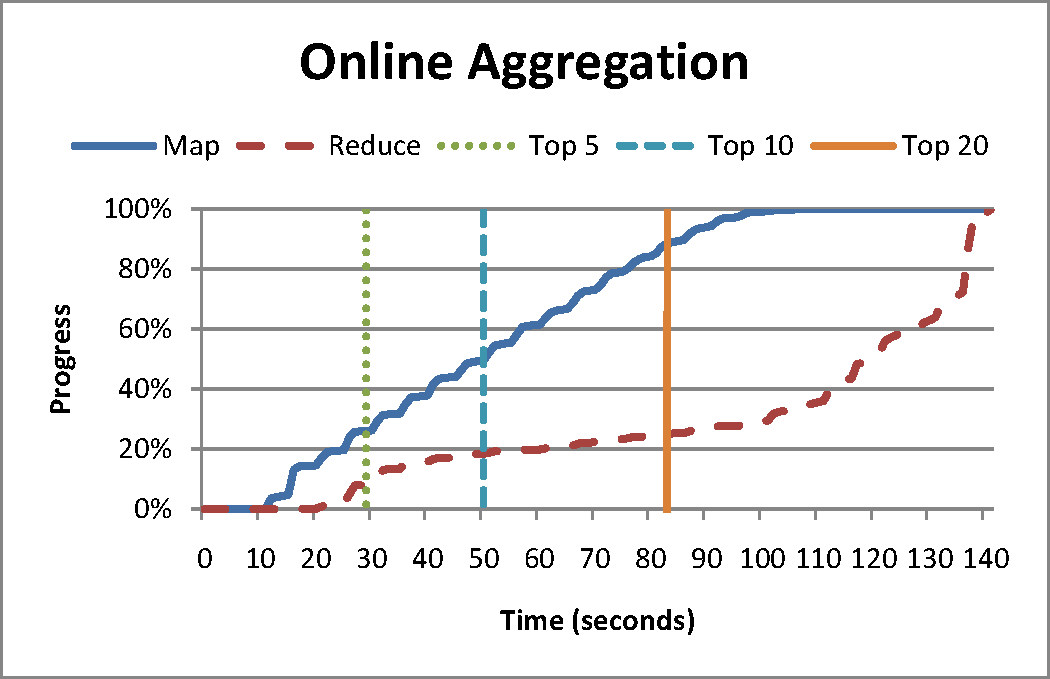
\includegraphics[width=0.7\linewidth]{figures/top100_online_wiki}
    \caption{Top-100 query over 5.5GB of Wikipedia article text. The vertical
      lines describe the increasing accuracy of the approximate answers produced
      by online aggregation.}
\label{fig:topkonlinewiki}
\vspace{-10pt}
\end{figure}

To evaluate the effectiveness of online aggregation, we performed two
experiments on Amazon EC2 using different data sets and query workloads.  In
our first experiment, we wrote a ``Top-$K$'' query using two MapReduce jobs:
the first job counts the frequency of each word and the second job selects the
$K$ most frequent words.  We ran this workload on 5.5GB of Wikipedia article
text stored in HDFS, using a 128MB block size.  We used a 60-node EC2 cluster;
each node was a ``high-CPU medium'' EC2 instance with 1.7GB of RAM and 2
virtual cores.  A virtual core is the equivalent of a 2007-era 2.5Ghz Intel
Xeon processor.  A single EC2 node executed the Hadoop \JT\ and the HDFS \NN,
while the remaining nodes served as slaves for running the {\TT}s and HDFS
{\DN}s.

% To evaluate inter-job dataflow with online aggregation we wrote a
% Top-$K$ query using two MapReduce jobs and executed it on 5.5GB of
% Wikipedia article text. The first job performs a wordcount on the
% words contained in each article.  A reducer from the first job will
% output a list of the Top-$K$ words observed in its partition. The key
% in this output is the word, and the value is the word count. Each map
% task in the subsequent job is assigned to an output from a single
% reduce task. The map function reverses the key-value order, and sends
% that result (sorted by count in descending order) to a single reduce
% task.  The single reduce task merges the sorted lists from each mapper
% and returns the first $K$ words.

% nrc: What does this experiment have to do with online aggregation?
% Figure~\ref{fig:topkwiki} reports the result of a Top-100 query over
% 5.5GB of Wikipedia article text. The left graph represents the
% blocking case as indicated by the idle period in the progress of the
% reduce tasks. The first map tasks finish around 100 seconds into the
% job, which is where the reduce tasks begin to make progress. The
% right graph shows a more balanced load. The reduce tasks
% being receiving mapper output almost immediately following the job
% execution, contributing to the early completion time of the job.

Figure~\ref{fig:topkonlinewiki} shows the results of inter-job online
aggregation for a Top-100 query.  Our accuracy metric for this experiment is
post-hoc --- we note the time at which the Top-$K$ words in the snapshot are
the Top-$K$ words in the final result.  Although the final result for this job
did not appear until nearly the end, we did observe the Top-5, 10, and 20
values at the times indicated in the graph.  The Wikipedia data set was biased
toward these Top-K words (e.g., ``the'', ``is'', etc.), which remained in their
correct position throughout the lifetime of the job.

\subsubsection{Approximation Metrics}

\begin{figure*}[ht]
\ssp
  \centering
  \subfloat[][Relative approximation error over time]{\label{fig:approx-relative}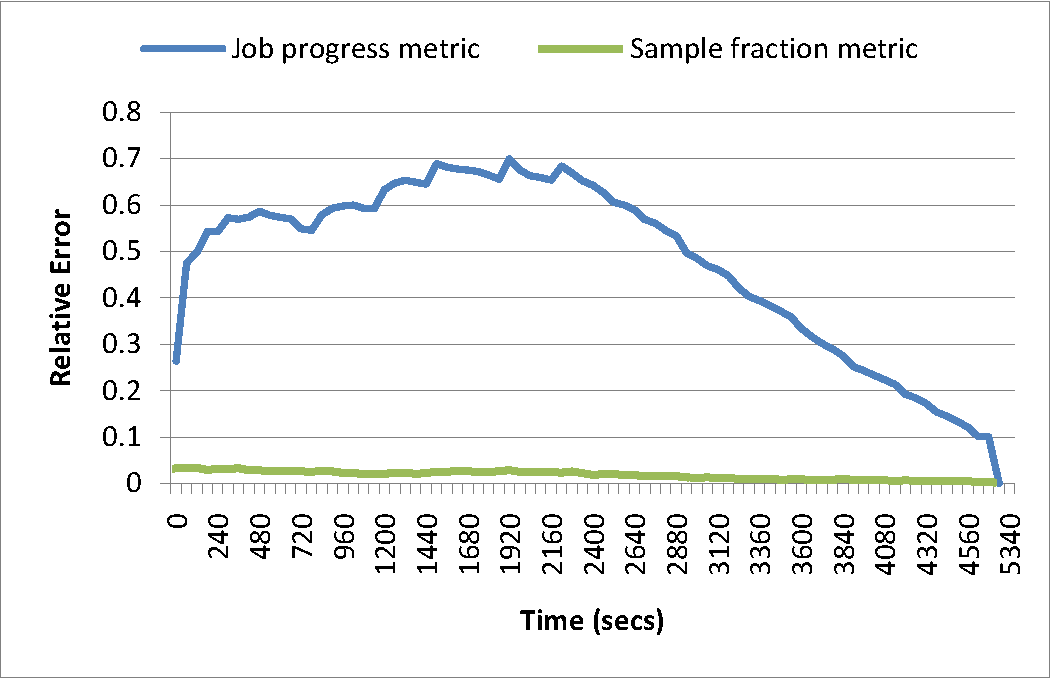
\includegraphics[width=0.48\linewidth]{figures/aprx-click-hour.pdf}}
  \subfloat[][Example approximate answer]{\label{fig:approx-hour}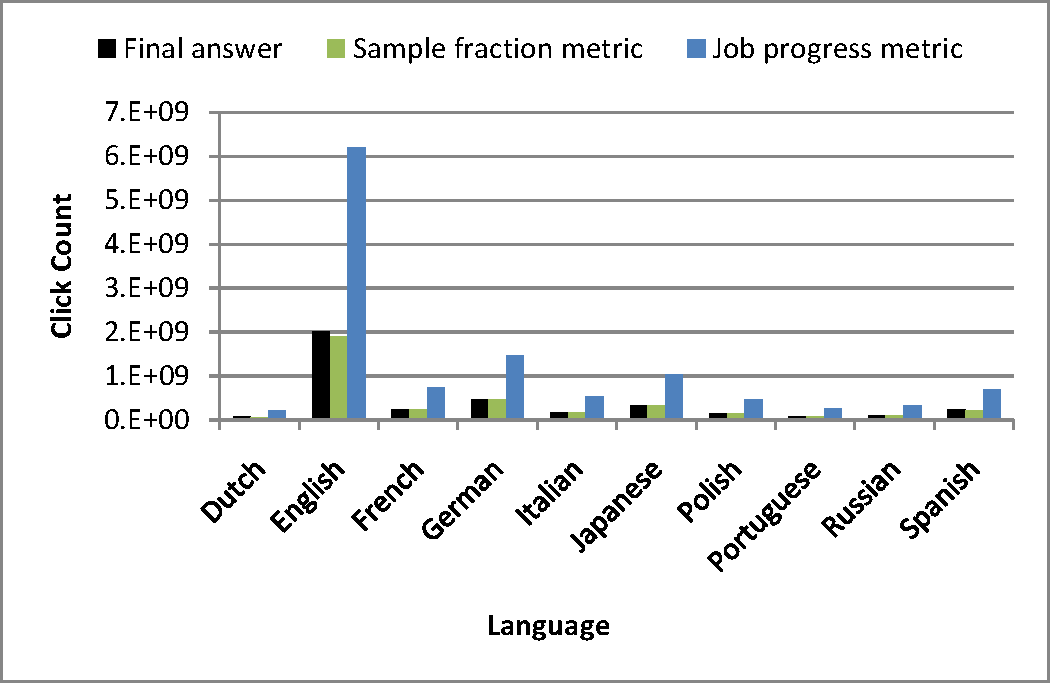
\includegraphics[width=0.48\linewidth]{figures/aprx-click-hour-actual.pdf}}
  \caption{Comparison of two approximation
    metrics. Figure~\protect\subref{fig:approx-relative} shows the relative error for
    each approximation metric over the runtime of the job, averaged over all
    groups. Figure~\protect\subref{fig:approx-hour} compares an example approximate
    answer produced by each metric with the final answer, for each language and for a single hour.}
\label{fig:approx}
\end{figure*}

In our second experiment, we considered the effectiveness of the job progress
metric described in Chapter~\ref{ch:hop:sec:online-metric}. Unsurprisingly, this metric
can be inaccurate when it is used to estimate the accuracy of the approximate
answers produced by online aggregation. In this experiment, we compared the job
progress metric with a simple user-defined metric that leverages knowledge of
the query and data set. HOP allows such metrics, although developing such a
custom metric imposes more burden on the programmer than using the generic
progress-based metric.

We used a data set containing seven months of hourly page view statistics for
more than 2.5 million Wikipedia articles~\cite{wikistats}. This constituted
320GB of compressed data (1TB uncompressed), divided into 5066 compressed
files. We stored the data set on HDFS and assigned a single map task to each
file, which was decompressed before the map function was applied.

We wrote a MapReduce job to count the total number of page views for each
language and each hour of the day. In other words, our query grouped by language
and hour of day, and summed the number of page views that occurred in each
group. To enable more accurate approximate answers, we modified the map function
to include the fraction of a given hour that each record represents. The reduce
function summed these fractions for a given hour, which equated to one for all
records from a single map task. Since the total number of hours was known ahead
of time, we could use the result of this sum over all map outputs to determine
the total fraction of each hour that had been sampled. We call this user-defined
metric the ``sample fraction.''

To compute approximate answers, each intermediate result was scaled up using two
different metrics: the generic metric based on job progress and the sample
fraction described above. Figure~\ref{fig:approx-relative} reports the relative
error of the two metrics, averaged over all groups. Figure~\ref{fig:approx-hour}
shows an example approximate answer for a single hour using both metrics
(computed two minutes into the job runtime). This figure also contains the final
answer for comparison. Both results indicate that the sample fraction metric provides a
much more accurate approximate answer for this query than the progress-based
metric.

Job progress is clearly the wrong metric to use for approximating the final
answer of this query. The primary reason is that it is too coarse of a
metric. Each intermediate result was computed from some fraction of each
hour. However, the job progress assumes that this fraction is uniform across all
hours, when in fact we could have received much more of one hour and much less
of another. This assumption of uniformity in the job progress resulted in a
significant approximation error. By contrast, the sample fraction scales the
approximate answer for each group according to the actual fraction of data seen for
that group, yielding much more accurate approximations.

\section{Continuous Queries}
\label{ch:hop:sec:continuous}

MapReduce is often used to analyze streams of constantly-arriving
data, such as URL access logs~\cite{mapreduce-osdi} and system console
logs~\cite{sosp-mining}. Because of traditional constraints on MapReduce, this 
is done in large batches that can only provide periodic views of activity.
This introduces
significant latency into a data analysis process that ideally should run in 
near-real time. It is also
potentially inefficient: each new MapReduce job does not have access
to the computational state of the last analysis run, so this state
must be recomputed from scratch. The programmer can manually save the
state of each job and then reload it for the next analysis operation,
but this is labor-intensive.

Our pipelined version of Hadoop allows an alternative architecture:
MapReduce jobs that run {\em continuously}, accepting new data as it
becomes available and analyzing it immediately. This allows for near-real-time
analysis of data streams, and thus
allows the MapReduce programming model to be applied to domains such
as environment monitoring and real-time fraud detection.

In this section, we describe how HOP supports continuous MapReduce
jobs, and how we used this feature to implement a rudimentary
cluster monitoring tool.

\subsection{Continuous MapReduce Jobs}
A bare-bones implementation of continuous MapReduce jobs is easy to
implement using pipelining. No changes are needed to implement
continuous map tasks: map output is already delivered to the
appropriate reduce task shortly after it is generated. We added an
optional ``flush'' API that allows map functions to force their current
output to reduce tasks. When a reduce task is unable to accept such data, the mapper framework
stores it locally and sends it at a later time. 
With proper scheduling of reducers, this API allows a map task to ensure that an output record is promptly sent to the appropriate
reducer.

To support continuous reduce tasks, the user-defined reduce function
must be periodically invoked on the map output available at that
reducer. Applications will have different requirements for how
frequently the reduce function should be invoked; possible choices
include periods based on wall-clock time, logical time (e.g., the
value of a field in the map task output), and the number of input rows
delivered to the reducer. The output of the reduce function can be
written to HDFS, as in our implementation of online
aggregation. However, other choices are possible; our prototype system
monitoring application (described below) sends an alert via email if
an anomalous situation is detected.

In our current implementation, the number of map and reduce tasks is
fixed, and must be configured by the user. This is clearly
problematic: manual configuration is error-prone, and many stream
processing applications exhibit ``bursty'' traffic patterns, in which
peak load far exceeds average load. In the future, we plan to add
support for elastic scaleup/scaledown of map and reduce tasks in
response to variations in load.

\subsubsection{Fault Tolerance}
In the checkpoint/restart fault-tolerance model used by Hadoop, mappers retain
their output until the end of the job to facilitate fast recovery from reducer
failures. In a continuous query context, this is infeasible, since mapper
history is in principle unbounded.  However, many continuous reduce functions
(e.g., 30-second moving average) only require a suffix of the map output stream.
This common case can be supported easily, by extending the \JT\ interface to
capture a rolling notion of reducer consumption.  Map-side spill files are
maintained in a ring buffer with unique IDs for spill files over time. When a
reducer commits an output to HDFS, it informs the \JT\ about the {\em run} of
map output records it no longer needs, identifying the run by spill file IDs and
offsets within those files.  The \JT\ can then tell mappers to garbage collect
the appropriate data.

In principle, complex reducers may depend on very long (or infinite) histories of map records to accurately reconstruct their internal state.  In that case, deleting spill files
from the map-side ring buffer will result in potentially inaccurate recovery after faults.  Such scenarios can be handled by having reducers checkpoint internal state to HDFS, along with markers for the mapper offsets at which the internal state was checkpointed.  The MapReduce framework can be extended with APIs to help with state serialization and offset management, but it still presents a programming burden on the user to correctly identify the sensitive internal state.  That burden can be avoided by more heavyweight process-pair 
techniques for fault-tolerance, but those are quite complex and use significant resources~\cite{flux-ft}.  In our work to date we have focused on cases where reducers can be recovered from a reasonable-sized history at the mappers, favoring minor extensions to the simple fault-tolerance approach used in Hadoop.

\subsection{Prototype Monitoring System}
\label{ch:hop:sec:monitor}

Our monitoring system is composed of {\em agents} that run on each monitored
machine and record statistics of interest (e.g., load average, I/O operations
per second, etc.). Each agent is implemented as a continuous map task: rather
than reading from HDFS, the map task instead reads from various system-local
data streams (e.g., \texttt{/proc}).

Each agent forwards statistics to an {\em aggregator} that is implemented as a
continuous reduce task. The aggregator records how agent-local statistics evolve
over time (e.g., by computing windowed-averages), and compares statistics
between agents to detect anomalous behavior. Each aggregator monitors the agents
that report to it, but might also report statistical summaries to another
``upstream'' aggregator. For example, the system might be configured to have an
aggregator for each rack and then a second level of aggregators that compare
statistics between racks to analyze datacenter-wide behavior.

\subsubsection{Evaluation}
\begin{figure}[t]
\ssp
  \centering
  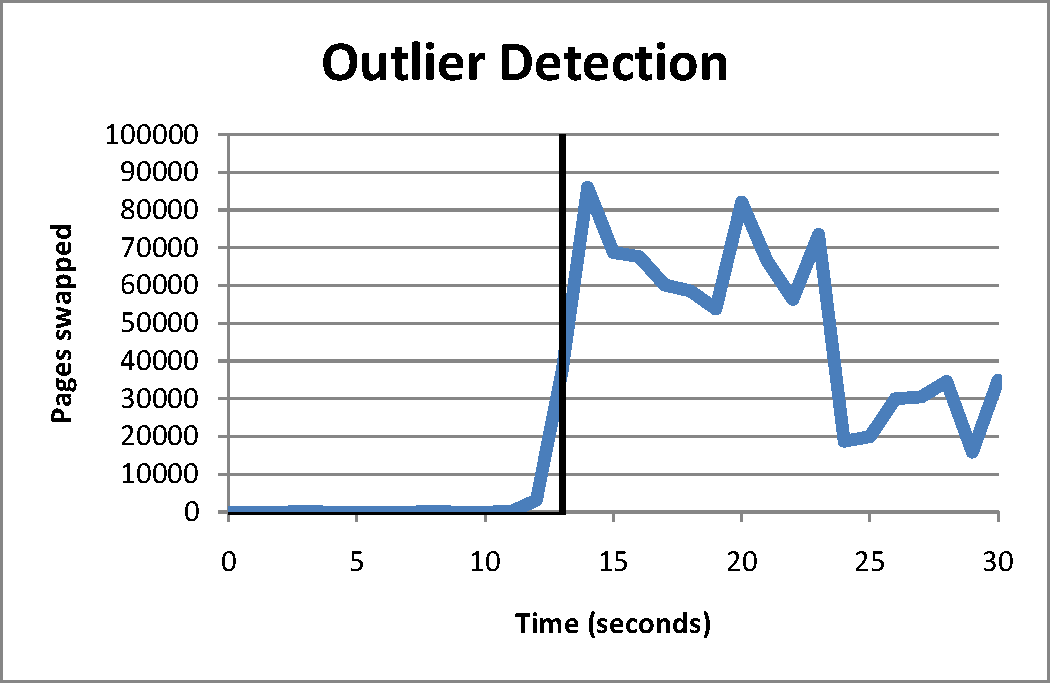
\includegraphics[scale=0.6]{figures/continue.pdf}
  \caption{Number of pages swapped over time on the thrashing host, as reported
    by \texttt{vmstat}.  The vertical line indicates the time at which the alert
    was sent by the monitoring system.}
\label{fig:outlier}
\end{figure}

To validate our prototype system monitoring tool, we constructed a
scenario in which one member of a MapReduce cluster begins thrashing
during the execution of a job. Our goal was to test how quickly our
monitoring system would detect this behavior. The basic mechanism is
similar to an alert system one of the authors implemented at an
Internet search company.

We used a simple load metric (a linear combination of CPU utilization,
paging, and swap activity). The continuous reduce function maintains
windows over samples of this metric: at regular intervals, it
compares the 20 second moving average of the load metric for each host
to the 120 second moving average of all the hosts in the cluster
{\em except} that host.  If the given host's load metric is more
than two standard deviations above the global average, it is
considered an outlier and a tentative alert is issued.  To dampen
false positives in ``bursty'' load scenarios, we do not issue an alert
until we have received 10 tentative alerts within a time window.

We deployed this system on an EC2 cluster consisting of 7 ``large''
nodes (large nodes were chosen because EC2 allocates an entire
physical host machine to them). We ran a wordcount job on the 5.5GB Wikipedia
data set, using 5 map tasks and 2 reduce tasks (1 task per host). After
the job had been running for about 10 seconds, we selected a node
running a task and launched a program that induced thrashing.

We report detection latency in Figure~\ref{fig:outlier}. The vertical bar
indicates the time at which the monitoring tool fired a (non-tentative)
alert. The thrashing host was detected very rapidly---notably faster than the
5-second {\TT}-{\JT} heartbeat cycle that is used to detect straggler tasks in
stock Hadoop. We envision using these alerts to do early detection of stragglers
within a MapReduce job: HOP could make scheduling decisions for a job by running
a secondary continuous monitoring query. Compared to out-of-band monitoring
tools, this economy of mechanism---reusing the MapReduce infrastructure for
reflective monitoring---has benefits in software maintenance and system
management.

\section{\BOOM-MR port}
\label{ch:hop:sec:boom}

This chapter describes our port of the \BOOM-MR (Chapter~\ref{ch:boom}) to HOP.
Using \BOOM-MR, we developed alternative scheduling policies, written in
\OVERLOG, that made use of statistics provided by the monitoring system
described in Chapter~\ref{ch:hop:sec:monitor}.  In
Chapter~\ref{ch:hop:sec:jolport}, we describe the port of \JOL to the
scheduling component of the HOP \JT.  Chapter~\ref{ch:hop:sec:jolmonitor}
describes the interface between the monitoring system and \JOL, which enabled
the use of the monitoring results in our declarative scheduling logic.  In
Chapter~\ref{ch:hop:sec:speculation}, we present an \OVERLOG rule that monitors
tasks for anomalous behavior~\cite{hopdemo}, spawning a backup/speculative task
when alerted to a potential issue.

\subsection{Scheduling HOP with \JOL}
\label{ch:hop:sec:jolport}

HOP is based on Hadoop 19.2, which defines an extensible interface to the \JT
scheduler component, allowing alternative scheduler implementations.  This made
the port of \JOL to HOP trivial: the entire port consisted of $55$ lines of
Java glue code that implemented the \JOL harness, and \OVERLOG code that
performed the basic scheduling policy described in Chapter~\ref{ch:boom}.  We
also altered the job relation (described in Table~\ref{ch:boom:tbl:hcatalog})
to include an attribute for the job type: pipelining/blocking, online
aggregation, or continuous.  We then added three scheduling policy rules that
were specific to online aggregation and continuous jobs.

\subsubsection{\JOL port}
\begin{figure*}
\ssp
\begin{minipage}{\linewidth}
\centering
\begin{verbatim}
public abstract class TaskScheduler implements Configurable {
   ...
   
  public abstract List<Task> 
  	assignTasks(TaskTrackerStatus taskTracker) throws IOException;
}
\end{verbatim}
\end{minipage}
\caption{Task scheduler interface. Not all methods shown.}
\label{ch:hop:fig:taskscheduler}
\end{figure*}


In Hadoop 19.2, the \JT makes use of an interface called the {\em
TaskScheduler} to implement alternative task scheduling policies.
Figure~\ref{ch:hop:fig:taskscheduler} shows a partial view of this interface,
which contains the method \ol{assignTasks} that is passed a \TT status object
and returns a list of tasks that should be scheduled.  This method is called by
the \JT during a {\em heartbeat} exchange with a \TT.

Our implementation of the \ol{assignTasks} method transforms the \TT status
object into a tuple that updates the \ol{taskTracker} relation in
Table~\ref{ch:boom:tbl:hcatalog}.  In response to this update, the scheduling
rules enter a fixpoint computation, during which it may assign task attempts to
the given \TT.  Any updates to the {\em schedule} relation (see rule \ol{s5} in
Figure~\ref{ch:boom:fig:schedule}) will trigger a (pre-registered) Java
listener that translates the update into a {\em Task} object, which the
\ol{assignTasks} method accumulates in a {\em List} object that is returned by
the \ol{assignTasks} method at the end of the fixpoint.

\subsubsection{Job submission interface}

The Hadoop {\JT} interface for submitting jobs had to be retrofitted to support
pipelining between jobs.  In regular Hadoop, jobs are submitted one at a time;
a job that consumes the output of one or more other jobs cannot be submitted
until the producer jobs have completed.  To support this, we modified the
Hadoop job submission interface to accept a list of jobs, where each job in the
list depends on the job before it.  The client interface traverses this list,
annotating each job with the identifier of the job that it depends on.  We then
added a new table to the declarative scheduler that captured inter-job
dependencies.  The job scheduling rules use this table to co-schedule jobs with
their dependencies, giving slot preference to ``upstream'' jobs over the
``downstream'' jobs they feed.  As we note in Chapter~\ref{ch:conclusion},
there are many interesting options for scheduling pipelines or even DAGs of
such jobs that we plan to investigate in future.


\subsubsection{Online aggregation and continuous job scheduling policies}

\begin{figure}
\ssp
\centering
\begin{lstlisting}
h1 unscheduledReduceTasks(JobId, a_count<TaskId>) :-
   job(JobId, JType, ...),
   task(JobId, TaskId, TType, Status, ...),
   JType == JobType.ONLINE, TType == TaskType.REDUCE,
   Status.state() != TaskState.RUNNING;

h2 canScheduleMaps(JobId) :-
   unscheduledReduceTasks(JobId, Count),
   Count == 0;

h3 canScheduleMaps(JobId) :-
   job(JobId, Type, ...),
   Type != JobType.ONLINE;
\end{lstlisting}
\caption{\label{ch:hop:fig:schedmaps} Counts the number of reduce tasks that are not running and 
only schedules map tasks from an online job when this count is zero.}
\end{figure}

Online aggregation and continuous jobs rely on a scheduling policy that ensures
the execution of the entire pipeline.  In the case of online aggregation, a
more complete pipeline provides more accurate estimates since unscheduled
partitions (i.e., groups) may contain important data.  For continuous jobs,
scheduling the entire pipeline is a requirement in order to avoid the memory
pressure in storing the (continuously arriving) data for an unscheduled
operator.  We enforced this constraint with by a policy that scheduled reduce
tasks before any map tasks in the same job (assuming sufficient slot capacity).

Figure~\ref{ch:hop:fig:schedmaps} shows three rules that together determine
when a job is allowed to schedule map tasks.  A separate admission controller
rule ensured that the number of reduce tasks for an online aggregation or
continuous job fit within the current cluster-wide slot capacity.  For each
job, rule \ol{h1} counts the number of reduce tasks not currently running.  If
the job type is ``online'' then rule \ol{h2} will add the fact that map tasks
can be scheduled when the number of non-running map tasks is equal to zero.
Rule \ol{h3} applies to the map tasks in all other job types; it simply removes
this scheduling constraints on those map tasks.  The \ol{canScheduleMaps}
predicate is included in the rule that determines the scheduling of map tasks
(e.g., rule \ol{s4} in Figure~\ref{ch:boom:fig:schedule}).

\section{Real-time monitoring with \JOL}
\label{ch:hop:sec:jolmonitor}

After porting \BOOM-MR to HOP, we started writing scheduler policies based on
the real-time monitoring information supplied by our monitoring job.  In order
to do this, we needed to import the results of our MapReduce monitoring job
into \JOL as relations.  Here, we further describe the MapReduce job that
continuously monitors HOP and its interface to \JOL.  We then present an alert
system that detects outlier measurements in map and reduce task execution
attempts.  We conclude our discussion with a new task speculation policy that
is based on our alert system.

\subsection{MapReduce monitoring job}

\begin{table}
\ssp
\centering
\begin{tabular}{|l|l|l|} \hline
\textit{Measure}    & \textit{Description}                 & \textit{Source} \\ \hline \hline
COMP\_EST        & Task estimated completion time  & \OVERLOG \\ \hline
USER\_CPU        & User CPU usage                   & /proc/stat, /proc/[pid]/stat \\ \hline
SYS\_CPU           & System CPU usage              & /proc/stat, /proc/[pid]/stat \\ \hline
RSS                       & Resident set memory size   & /proc/[pid]/stat   \\ \hline
VSIZE                    & Estimated completion time  & /proc/[pid]/stat  \\ \hline
WRITE\_BYTES   & Number of bytes written       & /proc/[pid]/io  \\ \hline
READ\_BYTES   & Number of bytes read           & /proc/[pid]/io \\ \hline
NET\_OUT           & Network output                      & /proc/net/dev \\ \hline
NET\_IN               & Network input                        & /proc/net/dev \\ \hline
SWAP\_OUT       & Swaps out                              & /proc/vmstat  \\ \hline
SWAP\_IN           &  Swaps in                               & /proc/vmstat \\ \hline
PAGE\_OUT       & Pages out                               & /proc/vmstat \\ \hline
PAGE\_IN           & Pages in                                 & /proc/vmstat \\ \hline
\end{tabular}
\caption{HOP monitoring measurements.}
\label{ch:hop:tbl:measure}
\end{table}

The MapReduce job that monitors HOP is scheduled during the system bootstrap.
The job executes a single map task on each \TT in the cluster and some
number (based on the size of the cluster) of reduce tasks that group machine
and rack level statistics.  For example, we could schedule a single reduce task
per rack that aggregates the statistics gathered on that rack.

Table~\ref{ch:hop:tbl:measure} lists the measurements that we collected.  The
measurement name is given in the first column, followed by a measurement
description.  The last column identifies the location under \ol{/proc} where
the measurement was taken.  Process level measurements reside under
\ol{/proc/[pid]/}, where \ol{[pid]} represents the process identifier.  All
other measurements outside of \ol{/proc/[pid]/} refer to machine level
measurements with the exception of the estimated completion time, which is
derived from task level statistics in the \JT.

A map task gathers measurements by periodically reading the source location
(last column in Table~\ref{ch:hop:tbl:measure}) from the local file system.
For each measurement, the map task outputs a record \ol{<host name, time stamp,
pid, measurement name, measurement value>}.  For machine statistics, the map
task will set the $PID$ field to {\underline 0} e.g.,
\ol{<boom.cs.berkeley.edu, 12348234, {\underline 0}, NET\_OUT, 101>}.  The
record key for all map outputs is the identifier of the rack to which the
machine belongs.  If the cluster does not contain rack-level information then
the host name is used instead.  This ensures that a single reduce task will see
all measurements from a given rack or machine boundary.

\subsection{Monitoring with \OVERLOG}
\label{ch:hop:sec:omonitor}

\begin{table}
\ssp
\centering
\begin{tabular}{|l|l|l|} \hline
\textit{Name}    & \textit{Description} & \textit{Relevant attributes} \\ \hline\hline
machineStat    & Machine statistics   & \underline{Host}, \underline{Measure}, TimeStamp, Value \\ \hline
proccessStat   & Process statistics    & \underline{TaskId}, \underline{Pid}, \underline{Measure}, TimeStamp, Value \\ \hline
jobStat              & Job statistics            & \underline{JobId}, \underline{TaskType}, \underline{Measure}, StatContainer \\ \hline
taskStat            & Task statistics          & \underline{JobId}, \underline{TaskId}, \underline{Measure}, TaskType, Value \\ \hline
alert                   & Outlier task alerts   & \underline{TaskId}, \underline{TimeStamp}, \underline{Measure}, \\
                           &                                   & Description, Severity \\ \hline
\end{tabular}
\caption{\JOL monitoring relations.}
\label{ch:hop:tbl:monitorCatalog}
\end{table}

The output of the monitoring job is sent directly --- reduce tasks open a
back-channel TCP-socket --- to the \JOL instance running on the \JT.  The
receiver code translates the data packets into \JOL tuples, and inserts them
into monitoring relations defined in Table~\ref{ch:hop:tbl:monitorCatalog}.
The \ol{machineStat} and \ol{processStat} tables are populated by the data
packets received from the monitoring jobs.  The \ol{jobStat} and \ol{taskStat}
tables maintain statistics for jobs and tasks, respectively, and are derived by
\OVERLOG rules (Figures~\ref{ch:hop:fig:taskstat}
and~\ref{ch:hop:fig:jobstat}).  The \ol{alert} table contains outlier task
measurements, which depending on the severity can result in corrective action
e.g., execute a speculative task (Chapter~\ref{ch:hop:sec:speculation}).

\begin{figure}
\ssp
\centering
\begin{lstlisting}
/* Correlate process measurements to the actual map/reduce task */
ts1 taskStat(TaskId.getJobID(), TaskId, Measure, Type, TimeStamp, 
             Value) :-
    taskAttempt(TaskId, ... , TaskState.RUNNING, Pid),
    processStat(Host, Pid, Measure, TimeStamp, Value),
    Type := TaskId.isMap() ? TaskType.MAP : TaskType.REDUCE;
        
/* Compute the estimated completion time based on the task rate 
   of progress */
ts2 taskStat(JobId, TaskId, COMP_EST, TaskType, TimeStamp, CompEst) :-
    taskAttempt(TaskId, ... , Progress, ProgressRate, TaskState.RUNNING, 
                Pid),
    JobId := TaskId.getJobID(),
    Type := TaskId.isMap() ? TaskType.MAP : TaskType.REDUCE,
    CompEst := ProgressRate == 0 ? infinity : 
               (1f - Progress) / ProgressRate,
    TimeStamp := java.lang.System.currentTimeMillis();
\end{lstlisting}
\caption{\label{ch:hop:fig:taskstat} Rules for maintaining the \ol{taskStat} table.}
\end{figure}

Figure~\ref{ch:hop:fig:taskstat} contains two rules that together maintain the
\ol{taskStat} table.  The \ol{taskAttempt} table was extended to include the
task process identifier ($Pid$), which is supplied by the \TT executing the
task attempt.  The process identifier allows us to correlate a task in the
\ol{taskAttempt} table with process level measurements in the \ol{processStat}
table, as shown by rule \ol{ts1}.  A task's estimated completion time is based
on its current progress and progress rate: change in progress computed over \TT
heartbeat intervals.  Using the current progress and progress rate, rule
\ol{ts2} computes a rough estimate on the remaining time it will take for the
task to complete, which we have denoted as a COMP\_EST measurement --- stored
in the \ol{taskStat} table.

\begin{figure}
\ssp
\centering
\begin{lstlisting}
js1 taskStatList(JobId, TaskType, Measure, a_list<Value>) :-
    taskStat(JobId, TaskId, Measure, TaskType, TimeStamp, Value);

        
js2 jobStat(JobId, TaskType, Measure, Statistics) :-
    taskStatList(JobId, TaskType, Measure, TaskStatList),
    Statistics := new StatContainer(TaskStatList);
\end{lstlisting}
\caption{\label{ch:hop:fig:jobstat} Rules for maintaining the \ol{jobStat} relation.}
\end{figure}

Figure~\ref{ch:hop:fig:jobstat} contains the rules for maintaining the
\ol{jobStat} table.  The \ol{taskStatList} table, maintained by rule \ol{js1},
provides a list of measurement values for each job identifier, task type, and
measurement name.  The \ol{jobStat} table groups measurement values belonging
to the same job, task type, and measurement name.  A special Java object called
{\em StatContainer} is used to store each group of measurements.  The {\em
StatContainer} class defines methods for computing various metrics (e.g., mean,
median, stddev, etc.) from its list of measurement values.  Rule \ol{js2}
maintains the \ol{jobStat} table by initializing a {\em StatContainer} object
for each group of aggregated measurement values.


\subsection{Task alerts} 

\begin{figure}
\ssp
\centering
\begin{lstlisting}
a1 alert (TaskId, TimeStamp, Measure, Desc, Severity) :-
   taskStat(JobId, TaskId, Measure, TaskType, TimeStamp, TaskStat),
   jobStat(JobId, TaskType, Measure, JobStat),
   JobStat.outlier(Measure, TaskStat) == true,
   Desc := JobStat.description(Measure, TaskStat),
   Severity := JobStat.severity(Measure, TaskStat),
   TimeStamp := java.lang.System.currentTimeMillis();
\end{lstlisting}
\caption{\label{ch:hop:fig:outlier} Rule for detecting outlier tasks. }
\end{figure}

Figure~\ref{ch:hop:fig:outlier} contains a single rule that detects outlier
task by correlating the task measurement with information in the \ol{jobStat}
table.  We compare the measurements from tasks that belong to the same category
--- job and task type (map or reduce).  The $JobStat$ variable references a {\em
StatContainer} object for a given category, and it is used to determine if a
task belonging to that category is an outlier based on some metric e.g., $k$
deviations from the mean.  The $JobStat$ variable is also used to provide a
description and severity of outlier measurement.

\subsection{Alert based speculation policy} 
\label{ch:hop:sec:speculation}

\begin{figure}
\ssp
\centering
\begin{lstlisting}

s1 mostRecentCriticalAlert(TaskId, Measure, a_min<AlertTime>) :-
   alert(TaskId, AlertTime, Measure, Desc, Severity),
   Severity.contains("critical");  /* The alert is critical */

s2 schedule(Tracker, list<TaskId, MapSlots>) :-
   heartbeat(Tracker, TrackerStatus, MapSlots, _),
   MapSlots > 0,
   mostRecentCriticalAlert(TaskId, Measure, AlertTime)

   /* Ensure the alert is not too old (alert time < 10 seconds ago). */
   (java.lang.System.currentTimeMillis() - AlertTime) < 10000,

   /* The task's estimated time to completion is very high relative
      to equivalent tasks. */
   taskStat(JobId, TaskId, COMP_EST, TaskType, TimeStamp, TaskStat),
   jobStat(JobId, TaskType, COMP_EST, JobStat),
   TaskStat < JobStat.percentile(0.25),

   /* Schedule backup if host has split or task has no splits 
      (e.g., reduce) AND no backup task has been scheduled */
   task(JobId, TaskId, ..., Splits, ...), TaskId.isMap(),
   taskAttemptCount(TaskId, Count), Count == 1,
   InputSplits.contains(TrackerStatus.getHost());
\end{lstlisting}
\caption{\label{ch:hop:fig:speculation} 
Rule for map task speculation based on alert system data. Reduce task 
speculation rule is similar and therefore omitted. }
\end{figure}    
   
Figure~\ref{ch:hop:fig:speculation} contains a rule that reschedules map tasks
with any ``critical'' alerts that occurred recently; rule~\ol{s1} defines the
\ol{mostRecentCriticalAlert} relation.  Rule~\ol{s2} is evaluated at the \JT
whenever a {\em heartbeat} exchange occurs with some \TT.  The \ol{heartbeat}
predicate includes the name of the \TT, its status, and its spare map slot
capacity, which the rule ensures is greater than zero.  The rule joins the
\ol{heartbeat} with all critical alerts in the \ol{mostRecentCriticalAlert}
relation.  As an added precaution, we subsequently check that the alerted
task's estimated completion (\ol{COMP\_EST}) time is high relative to other
tasks in its category.  Finally, we ensure that the task has not already been
rescheduled and that the \TT contains the maps input data.


\subsection{Evaluation}

\begin{figure*}[ht]
\ssp
  \centering
  \subfloat[][Hadoop 19.2 task speculation policy]{\label{fig:spec-hadoop}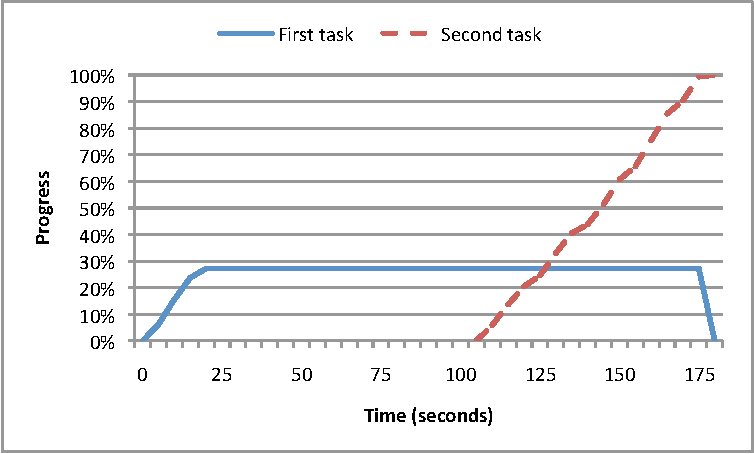
\includegraphics[width=0.48\linewidth]{figures/taskSpecPolicy_vanilla}}
  \subfloat[][HOP alert based task speculation policy]{\label{fig:spec-hop}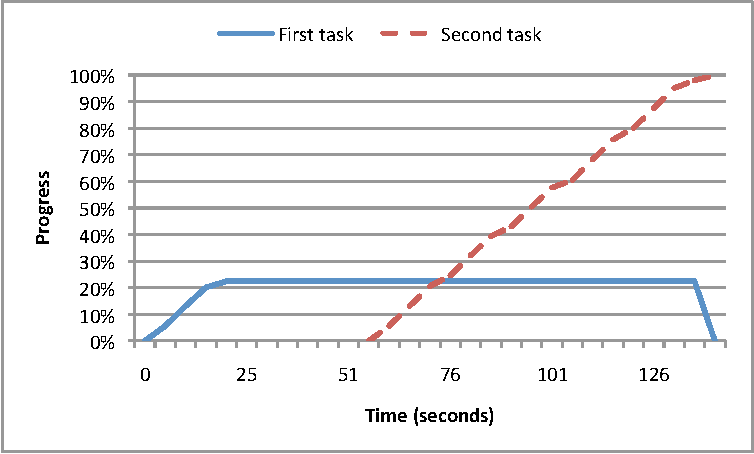
\includegraphics[width=0.48\linewidth]{figures/taskSpecPolicy_hop}}
  \caption{Compares speculation policies by plotting the starting point and progress of the faulty task (first task) and speculative task (second task).}
\label{fig:taskSpecPolicy}
\end{figure*}

We compared our alert based speculation policy with the speculation policy
implemented in unmodified Hadoop 19.2.  Our experiment executed a wordcount job
that contained a single faulty map task that would execute normally for a
minute before stalling out by sleeping for one second intervals between map
function invocations.  The input to the wordcount was 10GB of randomly
generated words, yielding 20 map tasks total.  We executed this job on a 20
node EC2 cluster and compared the time it took to initiate a speculative task
using our policy to the policy in unmodified Hadoop.

Figure~\ref{fig:taskSpecPolicy} shows the result of this experiment by plotting
the launch time and progress of the original (first) task and the backup
(second) task.  HOP's alert based speculation policy is able to detect the
faulty map task and execute a backup task in half the time of unmodified
Hadoop.  In unmodified Hadoop, a task is speculated based on its rate of
progress (relative to other tasks in its category).  We are able to further
extend this policy by including machine and process level statistics as further
evidence to speculate.  Indeed, our choice to speculate was not only based on a
high estimated time to completion but also a critically low ``user CPU'' value
and a critically low I/O activity.

The astute reader will notice however that the rate of progress for the second
task in HOP is less than that of unmodified Hadoop.  The reason for this is
that our monitoring jobs do add some extra load to the cluster.  Nevertheless,
in this instance, the overall job response time was slightly less (a few
seconds) in HOP due to the faster turn around time in our speculation policy.


\section{Related Work}
\label{ch:hop:sec:relwork}

This work relates to literature on parallel dataflow frameworks, online
aggregation, and continuous query processing.

\subsection{Parallel Dataflow}

Dean and Ghemawat's paper on Google's MapReduce~\cite{mapreduce-osdi} has
become a standard reference, and forms the basis of the open-source Hadoop
implementation.  The Google MapReduce design targets very large clusters where
the probability of worker failure or slowdown is high.  This led to their
elegant checkpoint/restart approach to fault-tolerance, and their lack of
pipelining.  Our work extends the Google design to accommodate pipelining
without significant modification to their core programming model or fault
tolerance mechanisms.

{\em Dryad}~\cite{dryad07} is a data-parallel programming model and runtime
that is often compared to MapReduce, supporting a more general model of acyclic
dataflow graphs.  Like MapReduce, Dryad puts disk materialization steps between
dataflow stages by default, breaking pipelines.  The Dryad paper describes
support for optionally ``encapsulating'' multiple asynchronous stages into a
single process so they can pipeline, but this requires a more complicated
programming interface.

It has been noted that parallel database systems have long provided partitioned
dataflow frameworks~\cite{pavlo09}, and recent commercial databases have begun
to offer MapReduce programming models on top of those
frameworks~\cite{aster,greenplum}.  Most parallel database systems can provide
pipelined execution akin to our work here, but they use a more tightly coupled
iterator and {\em Exchange} model that keeps producers and consumers
rate-matched via queues, spreading the work of each dataflow stage across all
nodes in the cluster~\cite{exchange}.  This provides less scheduling
flexibility than MapReduce and typically offers no tolerance to mid-query
worker faults.  Yang et al.\ recently proposed a scheme to add support for
mid-query fault-tolerance to traditional parallel databases, using a
middleware-based approach that shares some similarities with
MapReduce~\cite{osprey-icde}.

Logothetis and Yocum describe a MapReduce interface over a continuous query
system called {\em Mortar} that is similar in some ways to our
work~\cite{logoyocum08}.  Like HOP, their mappers push data to reducers in a
pipelined fashion.  They focus on specific issues in efficient stream query
processing, including minimization of work for aggregates in overlapping
windows via special reducer APIs.  They are not built on Hadoop, and explicitly
sidestep issues in fault-tolerance.

{\em Hadoop Streaming} is part of the Hadoop distribution, and allows map and
reduce functions to be expressed as UNIX shell command lines.  It does not
stream data through map and reduce phases in a pipelined fashion.

\subsection{Online Aggregation}

Online aggregation was originally proposed in the context of simple
single-table SQL queries involving ``Group By'' aggregations, a workload quite
similar to MapReduce~\cite{onlineagg}.  The focus of the initial work was on
providing not only ``early returns'' to these SQL queries, but also
statistically robust estimators and confidence interval metrics for the final
result based on random sampling.  These statistical matters do not generalize
to arbitrary MapReduce jobs, though our framework can support those that have
been developed.  Subsequently, online aggregation was extended to handle join
queries (via the {\em Ripple Join} method), and the {\em CONTROL} project
generalized the idea of online query processing to provide interactivity for
data cleaning, data mining, and data visualization tasks~\cite{ieeecontrol}.
That work was targeted at single-processor systems.  Luo et al.\ developed a
partitioned-parallel variant of Ripple Join, without statistical guarantees on
approximate answers~\cite{luo-ripple}.

In recent years, this topic has seen renewed interest, starting with Jermaine
et al.'s work on the {\em DBO} system~\cite{dbo}.  That effort includes more
disk-conscious online join algorithms, as well as techniques for maintaining
randomly-shuffled files to remove any potential for statistical bias in
scans~\cite{jermaine-shuffle}.  Wu et al.\ describe a system for peer-to-peer
online aggregation in a distributed hash table context~\cite{wu-vldb09}.  The
open programmability and fault-tolerance of MapReduce are not addressed
significantly in prior work on online aggregation.

An alternative to online aggregation combines precomputation with sampling,
storing fixed samples and summaries to provide small storage footprints and
interactive performance~\cite{gibbons98new}.  An advantage of these techniques
is that they are compatible with both pipelining and blocking models of
MapReduce.  The downside of these techniques is that they do not allow users to
choose the query stopping points or time/accuracy trade-offs
dynamically~\cite{ieeecontrol}.

\subsection{Continuous Queries}

In the last decade there was a great deal of work in the database research
community on the topic of continuous queries over data streams, including
systems such as Borealis~\cite{borealis}, STREAM~\cite{stream}, and
Telegraph~\cite{tcq-cidr}.  Of these, Borealis and Telegraph~\cite{flux-ft}
studied fault-tolerance and load balancing across machines.  In the Borealis
context this was done for pipelined dataflows, but without partitioned
parallelism: each stage (``operator'') of the pipeline runs serially on a
different machine in the wide area, and fault-tolerance deals with failures of
entire operators~\cite{borealisFT}.  SBON~\cite{sbon} is an overlay network
that can be integrated with Borealis, which handles ``operator placement''
optimizations for these wide-area pipelined dataflows.

Telegraph's {\em FLuX} operator~\cite{flux-ft,flux-lb} is the only work to our
knowledge that addresses mid-stream fault-tolerance for dataflows that are both
pipelined and partitioned in the style of HOP\@.  FLuX (``Fault-tolerant,
Load-balanced eXchange'') is a dataflow operator that encapsulates the
shuffling done between stages such as map and reduce.  It provides
load-balancing interfaces that can migrate operator state (e.g., reducer state)
between nodes, while handling scheduling policy and changes to data-routing
policies~\cite{flux-lb}.  For fault-tolerance, FLuX develops a solution based
on process pairs~\cite{flux-ft}, which work redundantly to ensure that operator
state is always being maintained live on multiple nodes.  This removes any
burden on the continuous query programmer of the sort we describe in
Chapter~\ref{ch:hop:sec:continuous}.  On the other hand, the FLuX protocol is
far more complex and resource-intensive than our pipelined adaptation of
Google's checkpoint/restart tolerance model.

\section{Summary}

In this chapter, we extended the batch-oriented execution model of MapReduce to
support pipelining between operators.  This enables a new suite of MapReduce
jobs that are able to perform online aggregation and continuous like queries.
Unlike much of the work on online aggregation, we do not focus here on
statistical guarantees because of the flexibility of the MapReduce programming
model.  These guarantees are crafted for specific SQL aggregates like SUMs,
COUNTs, and AVERAGEs, and modified to account for processing techniques like
the join algorithms used.  The focus of our work here is architectural: to
provide ``early returns'' interactions within the powerful scalability and
fault-tolerance facilities of MapReduce frameworks.  The statistical guarantees
from the literature only apply to SQL-style reduce functions; statistical
guarantees for other online reducers would need to be developed in a
case-by-case basis.  We expect that in many cases users will settle for simply
observing changes in the output of a job over time, and make their own
decisions about whether early returns are sufficient.

We leveraged our ability to run continuous MapReduce jobs in HOP by developing
a monitoring framework that provides near real-time machine and process level
statistics.  Our monitoring framework enabled new scheduling opportunities that
are based on such statistics.  Porting the declarative scheduler to HOP allowed
us to quickly prototype alternative policies in \OVERLOG where, in many cases,
adding new scheduling constraints translated into adding/removing a few rule
predicates.





\chapter[Conclusion and Future Extensions]{Conclusion and Future Extensions}
\label{ch:conclusion}

MapReduce has proven to be a popular model for large-scale parallel programming. Our Hadoop Online Prototype extends the applicability of the model to pipelining behaviors, while preserving the simple programming model and fault tolerance of a full-featured MapReduce framework.  This provides significant new functionality, including ``early returns'' on long-running jobs via online aggregation, and continuous queries over streaming data.  We also demonstrate benefits for batch processing:  by pipelining both within and across jobs, HOP can 
%achieve increased parallelism, improved system utilization, and 
reduce the time to job completion. 

In considering future work, scheduling is a topic that arises immediately.
Stock Hadoop already has many degrees of freedom in scheduling batch tasks across machines and time, and the introduction of pipelining in HOP only increases this design space.  First, pipeline parallelism is a new option for improving performance of MapReduce jobs, but needs to be integrated intelligently with both intra-task partition parallelism and speculative redundant execution for ``straggler'' handling.
%But given a fixed budget of task slots the cluster can run, pipeline depth has to be traded off against the number of concurrent partitions of a single dataflow stage (a single map or reduce).  We hope to expose these tradeoffs better via a closer analysis of the burstiness of resource consumption in stock Hadoop, and the resulting opportunity to smooth those bursts with pipelined parallelism.  
Second, the ability to schedule deep pipelines with direct
communication between reduces and maps (bypassing the distributed file
system) opens up new opportunities and challenges in carefully co-locating tasks from different jobs, to avoid communication when possible.  
%Finally, pipelining has tradeoffs with the use of map-side combiners.  As noted in Section~\ref{ch:hop:sec:pipelining}, for jobs that generate a small number of distinct reduce keys (e.g., genders), eager pipelining defeats the data reduction opportunities available with a blocking map-side combiner. For jobs with many reduce keys, or with no combiner available (e.g. Sort), aggressive pipelining may be a wise choice, to enable pipelined parallelism.  Since the number of distinct reduce keys is not typically known in advance, the choice of batch sizes for pipelining should be chosen in a dynamic fashion based on introspection during processing.  This introspection could be node-local, or could be a global decision fed by a continuous monitoring query of the sort illustrated in Section~\ref{ch:hop:sec:continuous}.  

Olston and colleagues have noted that MapReduce systems---unlike traditional databases---employ ``model-light'' optimization approaches that gather and react to performance information during runtime~\cite{olston-usenix08}.  The continuous query facilities of HOP enable powerful introspective programming interfaces for this: a full-featured MapReduce interface can be used to script performance monitoring tasks that gather system-wide information in near-real-time, enabling tight feedback loops for scheduling and dataflow optimization.  This is a topic we plan to explore further, including opportunistic methods to do monitoring work with minimal interference to outstanding jobs, as well as dynamic approaches to continuous optimization in the spirit of earlier work like Eddies~\cite{eddies} and FLuX~\cite{flux-lb}.

% Inter-job pipelining brings up some interesting opportunities for optimization as well. First, if we have a chain of two jobs, we can have the
% first job write its output to the local disk instead of going to HDFS. This
% saves the HDFS overhead at the expense of the risk of local disk failure.
% Since the intermediate data is relatively ephemeral, the window of risk may be tolerable in many cases. Second, we want to try scheduling maps of second job at nodes where reduces of the first job are running. This way data pipelining will be done locally and will not have to go through the network.

% Online aggregation changes some of the scheduling criteria in cases where there are not enough slots systemwide for all of a job's tasks.  Map and reduce tasks affect an online aggregation job differently: leaving map tasks unscheduled is akin to sampling the input file, whereas leaving reduce tasks unscheduled is akin to missing certain output keys -- some of which could be from groups with many inputs.  This favors reducers over mappers, at least during early stages of processing.  

% In order to improve early results of pipelined flows (e.g., for online aggregation), it is often desirable to prioritize ``interesting'' data in the pipeline, both at the mapper and reducer.  Online reordering of data streams has been studied in the centralized setting~\cite{juggle}, but it is unclear how to expose it in the MapReduce programming framework, with multiple nodes running in parallel -- especially if the data in the input file is not well randomized.  

%Continuous queries over streams raise many specific opportunities for optimizations, including sharing of work across queries on the same streams, and minimizing the work done per query depending on windowing and aggregate function semantics.  Many of these issues were previously considered for tightly controlled declarative languages on single machines~\cite{stream,tcq-cidr}, or for wide-area pipelined dataflows~\cite{borealis,sbon}, and would need to be rethought in the context of a programmable MapReduce framework for clusters.
 % many of which have been well-studied in the literature and should port naturally to a MapReduce setting, as demonstrated in initial work on the topic~\cite{logoyocum08}.  One key issue in the literature is the sharing of work across multiple queries on the same stream~\cite{precisionsharing,huebsch}; but prior work does not necessarily map well to a MapReduce framework, and the issue deserves more investigation.  
%Introspective system monitoring is a good driving application here, since it provides a well-motivated workload that developers of the system are well-motivated to study in depth.  

As a more long-term agenda, we want to explore using MapReduce-style programming for even more interactive applications.  As a first step, we hope to revisit interactive data processing in the spirit of the CONTROL work~\cite{ieeecontrol}, with an eye toward improved scalability via parallelism.  More aggressively, we are considering the idea of bridging the gap between MapReduce dataflow programming and lightweight event-flow programming models like SEDA~\cite{seda}.  Our HOP implementation's roots in Hadoop make it unlikely to compete with something like SEDA in terms of raw performance. However, it would be interesting to translate ideas across these two traditionally separate programming models, perhaps with an eye toward building a new and more general-purpose framework for programming in architectures like cloud computing and many-core.



% ===============================
% Part III: Back Matters
%           - bibliography
%           - appendix
%           - index
% ===============================

%\ssp
\bibliography{thesis}
%
% ======================================
% Main Document
%      - Part I:   Front Matters
%      - Part II:  Dissertation Chapters
%      - Part III: Back Matters
% ======================================

\documentclass[12pt,oneside,final]{ucthesis}
\def\dsp{\def\baselinestretch{2.0}\large\normalsize}
\dsp


% packages from Johan
% -------------------
%\usepackage{calc,babel,xspace}
%\usepackage{array,multirow,booktabs,units,url}
% -----------------------
% end packages from johan

\usepackage[final]{graphicx}
\usepackage{amstext,amssymb}
\usepackage{url}

\usepackage{times}
\usepackage{boxedminipage}
\usepackage{fancyhdr}
\usepackage{tabularx}
\usepackage{hhline}
\usepackage{color}
\usepackage{alltt}
\usepackage{xspace}
\usepackage{textcomp}
\usepackage{wrapfig}
\usepackage{balance}
\usepackage[protrusion=true,expansion=true]{microtype}
\usepackage{subfig}


%\includeonly{mimo}
\newcommand{\comment}[1]{}
\newtheorem{theorem}{Theorem}
\newtheorem{definition}{Definition}
\newtheorem{lemma}{Lemma}
\newtheorem{remark}{Remark}
\newtheorem{corollary}{Corollary}
\newcommand{\asn}{\ensuremath{:\,=}}
\newcommand{\defn}{\ensuremath{:\,=}}
\newcommand{\var}{\ensuremath{\operatorname{var}}}

\newcommand{\BOOM} {BOOM\xspace}
\newcommand{\BOOMA} {BOOM Analytics\xspace}
\newcommand{\BIGBOOM} {BOOM\xspace}
\newcommand{\JOL} {JOL\xspace}
\newcommand{\BIGJOL} {JOL\xspace}
\newcommand{\JT} {JobTracker\xspace}
\newcommand{\TT} {TaskTracker\xspace}
\newcommand{\NN} {NameNode\xspace}
\newcommand{\DN} {DataNode\xspace}
\renewcommand{\ttdefault}{cmtt}

\newcommand{\note}[1]{}

\def\compactify{\itemsep=0pt \topsep=0pt \partopsep=0pt \parsep=0pt}
 \let\latexusecounter=\usecounter
 \newenvironment{CompactItemize}
   {\def\usecounter{\compactify\latexusecounter}
    \begin{itemize}}
   {\end{itemize}\let\usecounter=\latexusecounter}
 \newenvironment{CompactEnumerate}
   {\def\usecounter{\compactify\latexusecounter}
    \begin{enumerate}}
   {\end{enumerate}\let\usecounter=\latexusecounter}

\renewcommand{\ttdefault}{cmtt}
\newcommand{\dataloglabel}[1]{\mbox{\bf #1:}\hfil}
\newenvironment{datalog}
  {\begin{list}{}%
      {\it \small \renewcommand{\makelabel}{\dataloglabel}%
    \setlength{\parsep}{-2pt}%
    }%
  }%
{\end{list}}
\newcommand{\datalogspace}{\textcolor[gray]{1}{.}\hspace{0.5in}}
\def\link{\texttt{\#link}\xspace}
\newcommand{\term}[1]{\textbf{#1}}
\newcommand{\stitle}[1]{\textbf{#1}---}

\newcommand{\ol}[1]{\texttt{\small #1}\xspace}

% this defines fancy header
% -------------------------
%\usepackage{fancyhdr}
%\pagestyle{fancy} \fancyhead{} \fancyfoot{} \if@twoside
%\fancyhead[LO]{\slshape\leftmark}
%\fancyhead[LE,RO]{\rmfamily\thepage}
%\fancyhead[RE]{\slshape\rightmark} \else
%\fancyhead[LO]{\slshape\leftmark}
%\fancyhead[RO]{\rmfamily\thepage} \fi


\begin{document}

% ========================
% Part I: Front Matters
%         - title page
%         - copyright
%         - abstract
%         - dedication
%         - TOC, LOF, LOT
%         - acknowledgment
% ========================

% ==========
% Title Page
% ==========

\title{Declarative Systems: Implementation, Optimization, and Beyond}
\author{Tyson Condie}
\degreeyear{2010} \degreesemester{} \degree{Doctor of Philosophy}
\chair{Professor Joseph M. Hellerstein}
\othermembers{Professor Michael J. Franklin \\
Professor Ion Stoica \\
Professor Tapan S. Parikh} \numberofmembers{4} 

\prevdegrees{B.A.
(University of California, Berkeley)  \\ M.S. (Stanford University) }
\field{Engineering-Electrical Engineering and Computer Sciences}
\campus{Berkeley}

 \maketitle \approvalpage \copyrightpage

%\renewcommand{\thepage}{\arabic{page}}

% ===============
% Thesis Abstract
% ===============
%\renewcommand{\thepage}{}
\begin{abstract}

There is a strong analogy between the Internet today, and database systems in the
1960's. Network protocol implementations involve complex procedural code, and
there is an increasing need to separate their specification from physical and logical
changes to components underneath them: network fabrics and architectures are being
redesigned for the next generation of Internet applications~\cite{geni05}. Hence the lessons of 
{\em data independence} and declarative approaches are very timely in this domain~\cite{networkind}, and are
reflected by recent interest in automatic network optimization and adaptation~\cite{grace-eurosys08}.
Moreover, we have observed that many networking tasks are naturally described in recursive
query languages like Datalog, because (a) they typically involve recursive graph traversals
(e.g., shortest-path computations)~\cite{loo-sigcomm05}, and (b) they are structured around
asynchronous messaging streams that \emph{join} with the current system state 
(e.g., "rendezvous" or "session" tables~\cite{p2:sosp, loo-sigmod06}).

Another area that has seen significant change during the early part of the $21^{st}$ century is the data center. During the late 1980's and into 
the 1990's, the client-server computing model prompted organizations to aggregate microcomputers in large computer rooms.
These early data centers were primarily used to control and operate all "in-house" information technology (IT) operations. 
In 2007, companies like Google and IBM, as well as a number of universities, embarked on a large scale {\em cloud computing} 
research project~\cite{lohr}. A primary focus for this new research direction was to commoditize the data center by enabling third-party
developers to simply and economically build and host applications on managed clusters.
Although, these cloud interfaces are convenient for launching multiple independent instances of traditional 
single-node services, writing truly distributed software remains a significant challenge.  Distributed applications still
require a developer to orchestrate concurrent computation and communication across machines, in a manner 
that is robust to delays and failures.  Writing and debugging such code is difficult even for experienced infrastructure
programmers, and drives away many creative software designers who might otherwise have innovative uses for 
cloud computing platforms.

This fast paced evolution in the Internet architecture and data center usage has enabled a new era
of applications in the form of Internet services such as Facebook, Google, MSN, Twitter, and Yahoo!. However,
many of these new applications are still being developed in programming languages that were specifically tailored to 
\emph{single instruction} computing models of the past~\cite{flynn}. In this dissertation, we demonstrate the 
utility of the declarative approach to developing the next generation of applications. We evaluate this conjecture 
with Datalog-based implementations of a host of functionalities at various levels of the system hierarchy 
(e.g., network protocols, query optimizers, and scheduling policies). Our declarative specifications of these
system applications are complied to dataflow runtime implementations reminiscent of traditional database query 
plans. We have found that using a declarative language often results in drastic reductions in code size 
($100x$ and more~\cite{chu-sensys07, p2:sosp, boom}) relative to procedural languages like C++. Perhaps more 
surprising, our declarative implementations are often quite intuitive: in many cases they are almost line-for-line 
translations of published pseudocode, suggesting that Datalog is indeed a good match for the 
application domain.

\abstractsignature
\end{abstract}

\setcounter{page}{1}
\renewcommand{\thepage}{\roman{page}}

\begin{frontmatter}


% ==========
% Dedication
% ==========

\begin{dedication}
\null\vfil {\large
\begin{center}
% To my wife and my advisor for giving me a chance.\\
%dedication.
\end{center}}
\vfil\null
\end{dedication}

%\tableofcontents \listoffigures \listoftables

% ===============
% Acknowledgments
% ===============

\begin{acknowledgements}




\end{acknowledgements}

\pagebreak\pagebreak \tableofcontents \listoffigures \listoftables
\end{frontmatter}

%\renewcommand{\thepage}{\arabic{page}}

% ================
% End of file:
% XEmacs variables
% ================

% Local Variables:
% TeX-master: "main.tex"
% End:






% ========================================
% Part II: Dissertation Chapters
%          - introduction (intro)
%          - circuit optimization (cctopt)
%          - micro-architectures (uarch)
%          - signal processing (sp-tech)
%          - cad flows (cad-flows)
%          - examples (svd-chip)
%          - experimental (test)
%          - conclusion (conclusion)
% ========================================

\setcounter{page}{1}
\renewcommand{\thepage}{\arabic{page}}\chapter[Dissertation Overview]{Dissertation Overview}
\label{ch:overview}

There has been renewed interest in recent years on applying declarative
languages to a variety of applications outside the traditional boundaries of
data management.  Examples include work on compilers~\cite{lam05context},
computer games~\cite{white-sigmod07}, security protocols~\cite{li-padl03}, and
modular robotics~\cite{ashley-iros07}.  Our work in this area began with the
{\em Declarative Networking} project, as instantiated in the {\em P2} system
for Internet overlays~\cite{p2:sosp, loo-sigmod06}.  This thesis represents the
final chapter of the P2 project and introduces a new exploration of {\em
declarative systems} in the context of {\em cloud
computing}~\cite{abovetheclouds}.

%A number of complex issues arise at the distributed layer, such as resource
%scheduling, the enforcement of distributed invariants (e.g., safety and
%liveness), consistency, availability, and fault-tolerance.  In this thesis, we
%focus on resource scheduling, and how it can be expressed compactly via a
%high-level declarative query language.  We also touch on an initial
%investigation of fault-tolerance in the context of MapReduce, which is another
%high-level dataflow language designed for the {\em
%cloud}~\cite{abovetheclouds}.

Our goal here is to explore systems programming in a high level declarative
language.  This effort is rooted in the {\em Declarative Networking}
project~\cite{boon-thesis}, which ignited the research direction of using a
declarative language to develop distributed software, specifically network
layer protocols and overlays for the next generation of Internet architectures.
In Chapter~\ref{ch:p2}, we review this influential work because it sets the
stage for this thesis.  Specifically, the declarative language \OVERLOG, which
I helped develop during this era, and continued to use throughout my work.  The
\OVERLOG language was accompanied by a runtime called P2, which automatically
compiled \OVERLOG programs into a dataflow-oriented runtime system.

The primary contributions presented in this dissertation begin in
Chapter~\ref{ch:evita}, where we describe our first declarative system
component -- Evita Raced, which is a declarative metacompiler implemented in
the final version of P2.  Evita Raced formulates the task of query compilation
as a query; written in the same declarative language (\OVERLOG) used by
``client'' queries, such as the various networking protocols from Loo, et
al.~\cite{loo-sigmod06, p2:sosp}.  The P2 compiler was first engineered to
compile query code into a relational format, thereby providing compilation
tasks (written in \OVERLOG) access to the logical query plan, and allowing the
ability to query and update that logical query plan.  We show that many
traditional database optimizations, like the magic-sets rewrite
(Chapter~\ref{ch:magic}), the System R dynamic program
(Chapter~\ref{ch:opt:sec:systemr}), and the Cascades branch-and-bound algorithm
(Chapter~\ref{ch:opt:sec:cascades}), can be fully expressed as \OVERLOG
queries.  Specifying these optimizations as \OVERLOG queries resulted in a more
concise representation of the {\em algorithm} as {\em code} and a dramatic
reduction in the overall development effort.  However, the pragmatics of
operating in a distributed environment led to a number of hacks that sacrificed
declarativity.  We reflect on the practicalities of system development and our
overall experience with Evita Raced in Chapter~\ref{ch:evitaend}.
 
In Chapter~\ref{ch:cloud}, we turn our attention to another system that has
gained in popularity recently --- Apache Hadoop~\cite{hadoop}.  Hadoop is an
open source software project that implements the MapReduce programming
model~\cite{mapreduce-osdi}.  In our work here, we investigated the Hadoop task
scheduling component, which is housed within the centralized coordinator of the
Hadoop MapReduce engine.  It is written in the (relatively) low-level Java
language~\cite{java}.  As we have already suggested, building and debugging
distributed software can be extremely difficult in such a procedural language.  We
conjecture that by adopting a {\em data-centric} approach to system design and
by employing {\em declarative} programming languages, a broad range of
distributed software functionality can be recast naturally in a data-parallel
programming model.  Our hope is that this model can significantly raise the
level of abstraction for programmers, improving code simplicity, speed of
development, ease of software evolution, and program correctness.

To evaluate this conjecture, we used the \OVERLOG language to implement an
API-compatible version of the Hadoop MapReduce scheduler.  Not only did we
achieve this goal using {\em orders of magnitude} fewer lines of code, our
implementation exhibits competitive performance, and extends Hadoop with
advanced fault-tolerance and scaling features that are typical for cloud
computing environments.  In Chapter~\ref{ch:hadoop}, we provide some background
material on MapReduce, which has emerged as a popular programming model for
writing data processing tasks in the cloud.  In Chapter~\ref{ch:boom}, we describe
our rewrite of the Hadoop MapReduce scheduling engine in a declarative language
and show that equivalent performance, fault-tolerance, and scalability
properties can be achieved in orders-of-magnitude less code.  In
Chapter~\ref{ch:hop}, we move beyond the batch-oriented execution model in
MapReduce to a more online execution model by pipelining data between system
operators.  This extension brings with it a number of scheduling challenges,
which we resolve in our declarative scheduling framework.  Finally, we conclude
in Chapter~\ref{ch:conclusion} with a discussion of future directions.





\section{Background}
\label{sec:background}

% XXX: should this be a distributed example?
\begin{figure}[t]
\begin{scriptsize}
\begin{lstlisting}
class ShortestPaths
  include Bud

  state do
    table :link, [:from, :to] => [:cost] (*\label{line:spaths-ddl}*)
    scratch :path, [:from, :to, :next_hop, :cost]
    scratch :min_cost, [:from, :to] => [:cost]
  end

  bloom do
    path <= link {|l| [l.from, l.to, l.to, l.cost]} (*\label{line:spaths-proj}*)
    path <= (link*path).pairs(:to => :from) do |l,p| (*\label{line:spaths-join-start}*)
      [l.from, p.to, l.to, l.cost + p.cost]
    end (*\label{line:spaths-join-end}*)

    min_cost <= path.group([:from, :to], min(:cost)) (*\label{line:spaths-group}*)
  end
end
\end{lstlisting}
\end{scriptsize}
\caption{All-pairs shortest paths in Bloom.}
\label{fig:bloom-spaths}
\end{figure}

In this section, we review the Bloom programming language and the CALM program
analysis.  We highlight a simple distributed program for which the CALM analysis
yields unsatisfactory results.

\subsection{Bloom}
\label{sec:bg-bloom}

Bloom is a Datalog-based domain-specific language (DSL) for distributed
programming~\cite{Alvaro2011,bloom}. The state of a Bloom program is represented
using \emph{collections} and computation is expressed as a bundle of declarative
\emph{statements}.  An instance of a Bloom program performs computation by
evaluating its statements over the contents of its local database. Bloom
instances communicate via asynchronous messaging, as described further below.

An instance of a Bloom program proceeds through a series of \emph{timesteps},
each containing three phases.\footnote{There is a precise declarative semantics
  for Bloom~\cite{dedalus}, but we describe the language operationally for the
  sake of exposition.} In the first phase, inbound events (e.g., network
messages) are received and represented as facts in collections. In the second
phase, the program's statements are evaluated over local state to compute all
the additional facts that can be derived from the current collection
contents. In some cases (described below), a derived fact is intended to achieve
a ``side effect,'' such as modifying local state or sending a network message.
These effects are deferred during the second phase of the timestep; the third
phase is devoted to carrying them out.

The initial implementation of Bloom, called \emph{Bud}, allows Bloom logic to be
embedded inside a Ruby program. Figure~\ref{fig:bloom-spaths} shows a Bloom
program represented as an annotated Ruby class. A small amount of imperative
Ruby code is needed to instantiate the Bloom program and begin executing it;
more details are available on the Bloom language website~\cite{bloom}.

\subsubsection{Data model}
\begin{table}[t]
\begin{tabular}{|l|p{2.32in}|}
\hline
\textbf{Name} & \textbf{Behavior }\\
\hline
\texttt{table} & Persistent storage.\\
\texttt{scratch} & Transient storage.\\
\texttt{channel} & Asynchronous communication. A fact derived into a \texttt{channel} appears in the
database of a remote Bloom instance at a non-deterministic future time.\\
\texttt{periodic} & Interface to the system clock.\\
\texttt{interface} & Interface point between software modules.\\
\hline
\end{tabular}
\caption{Bloom collection types.}
\label{tbl:bloom-collections}
\end{table}

The Bloom data model is based on \emph{collections}.  A collection is an
unordered set of \emph{facts}, akin to a relation in Datalog. The Bud prototype
adopts the Ruby type system rather than inventing its own; hence, a fact in Bud
is just an array of Ruby objects. Each collection has a \emph{schema}, which
declares the structure (column names) of the facts in the collection. A subset
of the columns in a collection form its \emph{key}: as in the relational model,
the key columns functionally determine the remaining columns. The collections
used by a Bloom program are declared in a \texttt{state} block. For example,
line~\ref{line:spaths-ddl} of Figure~\ref{fig:bloom-spaths} declares a
collection named \texttt{link} with three columns, two of which form the
collection's key. Ruby is a dynamically typed language, so keys and values in
Bud can hold arbitrary Ruby objects.

Bloom provides five collection types to represent different kinds of state
(Table~\ref{tbl:bloom-collections}). A \texttt{table} stores persistent data: if
a fact appears in a table, it remains in the table in future timesteps (unless it
is explicitly removed). A \texttt{scratch} contains transient data---the content
of scratch collections is emptied at the start of each timestep. Scratches are
akin to SQL views: they are often useful as a way to name intermediate results
or as a ``macro'' construct to enable code reuse. The \texttt{channel}
collection type enables communication between Bloom instances. The schema of a
channel has a distinguished \emph{location specifier} column (prefixed with
``\texttt{@}''); when a fact is derived for a channel collection, it appears in
the database of the Bloom instance at the address given by the location
specifier. The \texttt{periodic} and \texttt{interface} collection types do not
arise in our discussion in this paper; the interested reader is referred to the
Bloom website~\cite{bloom}.

\subsubsection{Statements}
\begin{table}
\begin{tabular}{|c|l|p{1.85in}|}
\hline
\textbf{Op} & \textbf{Name} & \textbf{Meaning} \\
\hline
\verb|<=| & \emph{merge} & lhs includes the content of rhs in the
current timestep \\
\hline
\verb|<+| & \emph{deferred merge} & lhs will include the content of rhs in the
next timestep \\
\hline
\verb|<-| & \emph{deferred delete} & lhs will not include the content of rhs
in the next timestep \\
\hline
\verb|<~| & \emph{async merge} & (remote) lhs will include the content of the
rhs at some non-deterministic future timestep\\
\hline
\end{tabular}
\caption{Bloom operators.}
\label{tbl:bloom-ops}
\end{table}

Each Bloom statement has one or more input collections and a single output
collection.  A statement takes the form: \\ \noindent
\mbox{\hspace{0.25in}\emph{$<$collection-identifier$>$ $<$op$>$
    $<$collection-expression$>$}}\\ \noindent
The left-hand side (lhs) is the name of the output collection and the right-hand
side (rhs) is an expression that produces a collection.  A statement defines how
the contents of the input collections should be transformed before being
included (via set union) in the output collection. Bloom allows the usual
relational operators to be used on the rhs (selection, projection, join,
grouping, aggregation, and negation), although it adopts a syntax intended to be
more familiar to imperative programmers. In Figure~\ref{fig:bloom-spaths},
line~\ref{line:spaths-proj} demonstrates projection,
lines~\ref{line:spaths-join-start}--\ref{line:spaths-join-end} perform a join
between \texttt{link} and \texttt{path} using the join predicate
\verb+link.to = path.from+ followed by a projection to four attributes, and
line~\ref{line:spaths-group} demonstrates grouping and aggregation. Bloom
statements appear in one or more \texttt{bloom} blocks. A Bloom program can also
include a \texttt{bootstrap} block, which contains statements that are evaluated
only once when a Bloom instance starts executing. \texttt{bootstrap} blocks are
typically used for initialization or configuration data.

Bloom provides several operators that determine \emph{when} the rhs will be
merged into the lhs (Table~\ref{tbl:bloom-ops}). The \verb|<=| operator performs
standard logical deduction: that is, the lhs and rhs are true at the same
timestep. The \verb|<+| and \verb|<-| operators indicate that facts will be
added or removed, respectively, from the lhs collection at the beginning of the
\emph{next} timestep. The \verb+<~+ operator specifies that the rhs will be merged into
the lhs collection at some non-deterministic future time. The lhs of a statement
that uses \verb+<~+ must be a channel; the \verb+<~+ operator captures
asynchronous messaging.

% XXX: does this need to be said?
Bloom allows recursion---i.e., the rhs of a statement can reference the lhs
collection, either directly or indirectly. As in Datalog, certain constraints
must be adopted to ensure that programs with recursive statements have a
sensible interpretation. For deductive statements (\verb+<=+ operator), we
require that programs be \emph{syntactically stratified}~\cite{Apt1988}: cycles
through negation or aggregation are not allowed (unless they contain a deferred
or asynchronous operator)~\cite{dedalus}.

\subsection{CALM analysis}
\label{sec:bg-calm}

Work on deductive databases has long drawn a distinction between
\emph{monotonic} and \emph{non-monotonic} logic programs. Intuitively, a
monotonic program only computes more information over time---it will never
``retract'' a previous conclusion in the face of new evidence.  In Bloom (and
Datalog), a simple conservative test for monotonicity is based on program
syntax: selection, projection, and join are monotonic, while aggregation and
negation are not.

The CALM theorem connects the theory of monotonic logic with the practical
problem of distributed consistency~\cite{Alvaro2011,Hellerstein2010}.  All
monotonic programs are ``eventually consistent'' or \emph{confluent}: for any
given input, all program executions result in the same final state regardless of
network non-determinism~\cite{Ameloot2011,dedalus-confluence}.  Hence, monotonic
logic is a useful building block for loosely consistent distributed programming.

According to the CALM theorem, distributed inconsistency may only occur at
\emph{points of order}: program locations where the output of an asynchronously
derived value is consumed by a non-monotonic operator.  This is because
asynchronous messaging results in non-deterministic arrival order, and
non-monotonic operators may be produce different conclusions when evaluated over
different subsets of their inputs.  For example, consider a Bloom program in
which collections $A$ and $B$ are fed by asynchronous channels and the program
sends a message whenever an element of $A$ arrives that is not in $B$. This
program is non-monotonic and exhibits non-confluent behavior: the messages sent
by the program will depend on the order in which the elements of $A$ and $B$
arrive.

We have implemented a conservative static program analysis in Bloom that follows
directly from the CALM theorem.  Programs that are free from non-monotonic
constructs are ``blessed'' as confluent: producing the same output on different
runs or converging to the same state on multiple distributed replicas.
Otherwise, programs are flagged as potentially inconsistent.  To achieve
consistency, the programmer either needs to rewrite their program to avoid the
use of non-monotonicity or introduce a coordination protocol to ensure that a
consistent ordering is agreed upon. Coordination protocols incur additional
latency and reduce availability in the event of network partitions, so in this
paper we focus on coordination-free designs---that is, monotonic programs.

\subsubsection{Limitations of set monotonicity}
The original formulation of the CALM theorem considered only programs that
compute more facts over time---that is, programs whose output \emph{sets} grow
monotonically. Many distributed protocols make progress over time, but their
notion of ``progress'' is often difficult to represent as a growing set of
facts. For example, consider the Bloom program in
Figure~\ref{fig:bloom-nm-quorum}. This program receives votes from a client
program (not shown) via the \texttt{vote\_chn} channel. Once at least
\texttt{QUORUM\_SIZE} votes have been received, a message is sent to a remote
node to indicate that quorum has been reached
(line~\ref{line:bloom-quorum-msg}). This program resembles a ``quorum vote''
subroutine that might be used by an implementation of Paxos~\cite{Lamport1998}
or quorum replication~\cite{Gifford1979}.

It is easy to see that this program makes progress in a semantically monotonic
fashion: the set of received votes grows and the size of the \texttt{votes}
collection can only increase, so once a quorum has been reached it will never be
retracted. Unfortunately, the current CALM analysis would regard this program as
non-monotonic because it contains aggregation (the grouping operation on
line~\ref{line:bloom-nm-quorum}).

To solve this problem, we need to introduce a notion of program values that
``grow'' according to a partial order other than set containment. We do this by
extending Bloom to operate over arbitrary lattices, rather than just the
set lattice.

%  We present a
% complete language in the following section, but the intuition can be observed in
% Figure~\ref{fig:lattice-quorum}. Votes are accumulated into a set lattice
% (line~\ref{line:quorum-set-accum}), but the size of the set is represented as an
% \texttt{lmax} lattice (line~\ref{line:quorum-lmax}): that is, a number that
% never decreases. Hence, a threshold test ``$\ge k$'' on an \texttt{lmax} lattice
% is monotonic map onto the boolean lattice: that is, the \texttt{quorum\_done}
% predicate goes from false to true (and then remains true).

\begin{figure}[t]
\begin{scriptsize}
\begin{lstlisting}
QUORUM_SIZE = 5
RESULT_ADDR = "example.org"

class QuorumVote
  include Bud

  state do
    channel :vote_chn, [:@addr, :voter_id]
    channel :result_chn, [:@addr]
    table   :votes, [:voter_id]
    scratch :cnt, [] => [:cnt]
  end

  bloom do
    votes      <= vote_chn {|v| [v.voter_id]}
    cnt        <= votes.group(nil, count(:voter_id)) (*\label{line:bloom-nm-quorum}*)
    result_chn <~ cnt {|c| [RESULT_ADDR] if c >= QUORUM_SIZE} (*\label{line:bloom-quorum-msg}*)
  end
end
\end{lstlisting}
\end{scriptsize}
\caption{A non-monotonic Bloom program that waits for a quorum of votes to be received.}
\label{fig:bloom-nm-quorum}
\end{figure}

%\documentclass[dvips,10pt]{article}
\usepackage{amsmath}
\usepackage{amssymb}
\usepackage{epsfig}
\usepackage{verbatim}
\usepackage{times}
\usepackage[bf,small,compact]{titlesec}

\date{}
\title{Dataflow Architecture for P2 \vspace{-1em}}

% Setup stuff
% Side margins:
\oddsidemargin 0in
\evensidemargin 0in

% Text width:
\textwidth 6.5in

% Top margin:
\topmargin -.25in

% Text height:
\textheight 8.5in

% Give footnotes a little more room:
%\renewcommand{\footnotesep}{5mm}

\author{Us Smarties}
\sloppy
\begin{document}
\maketitle
\begin{abstract}
Can we {\em please} close the door on this already?

\end{abstract}
\section{Introduction}
Lots of takes on dataflow arch in DB and NW communities.  DB query
engines.  OS support for NW ``Data Manipulation'' (in Clark and
Tennehouse's terminology) including Scout.  Network router toolkits
like Click.  Network/DB hybrids including Volcano's Exchange operator,
Telegraph's Fjords model, the architecture of PIER.

An effort here to taxonomize the design space for software dataflow
systems, and a description of an implementation in P2 that maximizes
flexibility in the model without sacrificing any efficiency with
respect to more constrained designs.

\section{Background Thoughts on Indirection: Space and Time}
Producer-Consumer ``handoff'' is most easily pictured as having two
agents rendezvous at the same place and time to transfer a datum.  But
co-location and simultaneity are not always possible to achieve in
practice -- particularly with networked machines, but even within the
confines of a single machine.

``Everything in CS can be solved with a level of indirection'' applies
here.  We often think of indirection in {\em space}, in which we free
the producer and consumer from agreeing {\em a priori} upon a spatial
  location.  This is typically done by providing a lookup mechanism
  for one or both parties to identify the current rendezvous location.

We can also achieve indirection in {\em time}, in which we free the
producer and consumer from agreeing {\em a priori} on a time for the
rendezvous.  This is achieved by persistence.  Note that persistence
can be leverage when either the producer or the consumer arrives at
the rendezvous first. The producer can place data into storage (a
queue, a mailbox, etc.) which holds the data until the consumer
arrives.  Alternatively, the consumer can place a forwarding handler
into storage in advance of the producer, so that when the producer
arrives it can invoke the data receipt logic.

(``Persistence'' has another meaning in common speech, which is akin
to the notion of ``retry'' or ``polling'' in networking.  Retry in the
absence of storage is a way of achieving simultaneity, and hence
removing indirection in time.  Typically, retry is not used alone,
however. It is combined with at least a modest amount of storage --
say 1 message worth -- to avoid the need for perfect simultaneity.
Instead, retry limits the latency of handoff and the rate-lag between
producer and consumer.)

\section{A Generic Dataflow Handoff Model}
We begin with a generic model in which two independent agents
(machines or processes) need to achieve handoff.  We ignore
indirection in space for the moment.

We assume a ``slot'' (a queue of size 1) for persistence.  This slot
can hold a tuple of the form $(desire, data, handler)$.  The $data$ is
(a handle for) the actual data to be transferred; the $handler$ is a
piece of code (a continuation, functor, function pointer, etc.) that
can be invoked.  We now enumerate the possible actions a producer or
consumer can take on the slot:

\begin{verbatim}
// I doubt this would compile in any language 
// but hopefully you see what I mean.  It's also not
// optimized to avoid copies or the like.
// Perhaps should convert to prose or 
// more pseudo-ish code to avoid getting
// nailed on the detail.
class slot {
  private boolean desire;
  private data;
  private return_code &handler;

  void put_desire { desire = true; }
  boolean check_desire { return desire; }
  void put_data(d)     { data = d; }
  void put_handler(h)  { handler = h; }

  void clear_slot() { desire = false; data = handler = NULL; }

  data get_data() { desire = false; d = data; data = NULL; return d; }
  return_code invoke_handler() { return handler(); }
}
\end{verbatim}

\subsection{Coupling Data and Control Flows}
One standard approach to dataflow architectures is to couple the
scheduling of the producer and consumer with the passage of data.  For
example, the standard database iterator model has consumers call
(i.e. directly schedule) producers, with data being returned on the
stack at the end of the producer's computation.  This is sometimes
called a ``pull'' model.  The opposite approach is also used in some
systems, in which producers call consumers, passing the data on the
call stack.

Both of these approaches can be achieved in our model with appropriate
scheduling of producer code, consumer code, and slot methods.  The
slot plays the role that would be played by the stack in the
function-call approach.  In these scenarios, the scheduler
deterministically orders the invocation of consumer and producer code
to achieve the coupling in time that is implicit in the function-call
approach.

\begin{verbatim}
Coupled Pull (iterator)
=======================
pull_consumer_prologue(); // calls slot.set_desire();
pull_producer_prologue(); // calls slot.put_data
pull_producer_epilogue();
pull_consumer_epilogue(); // calls get_data();


Coupled Push
============
push_producer_prologue(); // calls slot.put_data
push_consumer_prologue(); 
push_consumer_epilogue(); // calls get_data();
push_producer_epilogue();
\end{verbatim}

\subsection{Asynchronous Push and Pull}
In many scenarios, the arrival of data or of desires cannot be
controlled.  Hence the scheduling of producer and consumer code may be
deserving of more flexibility that in the coupled approaches we have
seen so far.  One example of this is a ``non-blocking pull'' model, in
which desire precedes data by some uncontrolled amount of time.  This
is the standard scenario in disk I/O requests.

\begin{verbatim}
Non-Blocking Pull
=================
// FIX TO CONSIDER THE PREFETCH SCENARIO AS WELL!
async_pull_consumer_prologue(); 
  // calls slot.put_desire, 
  // and slot.put_handler(async_pull_consumer_epilogue)

add async_pull_producer() to the run queue; 
  // eventually calls slot.put_data()
  // followed immediately by slot.invoke_handler()
\end{verbatim}

An alternative scenario is the ``non-blocking push'' model, in which
the producer may run ahead of the consumer.  This scenario arises in
network send environments, where the consumption of a packet has to
wait for a channel slot.

\begin{verbatim}
Non-Blocking Push
=================
// FIX TO CONSIDER BACKPRESSURE!
asynch_push_producer_prologue();
  // calls slot.put_data, 
  // and slot.put_handler(async_push_producer_epilogue)

add async_push_consumer() to the run queue;
  // eventually calls slot.get_data()
  // followed by slot.invoke_handler()
\end{verbatim}


\subsection{Completely Decoupled Producer/Consumer pairs}
\begin{itemize}
\item Asynch P/C with polling 
\item Asynch P/C with handlers
\item Mix and match polling/handlers?
\end{itemize}

\section{Multi-Operator Pipelines}

\section{From Events to Threads}
In the previous model we assumed that producers and consumers were
independent agents.  An alternative approach is to consider a
single-node, threaded architecture, in which we can (perhaps flexibly)
choose to connect multiple operators in a single thread via function
calls.  This essentially couples control-flow and dataflow for subsets
of the operators, as discussed above.

Argument here that Mothy's ``slot-as-thread-boundary'' approach can be
made to do everything we did up to now.  

Argument that it's more efficient to couple control and dataflow for
predictable operators.
\end{document}

\chapter[Declarative Optimization]{Declarative Optimization}
\label{ch:evita}

Declarative Networking has the potential to expand the lessons and impact of
database technologies into new domains, while reviving interest in classical
database topics like recursive query processing that have received minimal
attention in recent years.  Yet our own system was entirely implemented in an
imperative programming language: the initial version of the P2 runtime was
implemented in C++~\cite{p2:sosp}.  We asked ourselves whether Codd's vision
applies to our own efforts: can declarative programming improve the
implementation of declarative systems?

In this chapter, we put declarative systems ``in the mirror'' by investigating
a declarative implementation of one key component in any relational database
system, the query optimizer.  Specifically, we reimplemented the query
optimizer of P2 as a {\em metacompiler}: a compiler (optimizer) for the P2
language, \OVERLOG, that is itself written in \OVERLOG.  We named the resulting
implementation ``Evita Raced.''\footnote{``Evita Raced'' is almost
``Declarative'' in the mirror, but as with the \OVERLOG language itself, it
makes some compromises on complete declarativity.} Using Evita Raced, we
extended P2 with a number of important query optimization techniques it
formerly lacked, and found that our declarative infrastructure made this quite
elegant and compact.  As we will see in Section~\ref{ch:evita:sec:systemr}, our
implementation of the traditional System R dynamic programming algorithm
comprises only $38$ \OVERLOG rules ($225$ lines of code); our implementation of the
Magic-sets rewriting optimization for recursive queries is not only compact ($68$
rules, $264$ lines), but also nearly a direct translation of the description from
Ullman's course notes on the subject~\cite{ullmanNotes}.

The elegance of our approach was derived in part from the fact that many query
optimization techniques -- like many search algorithms -- are at heart
recursive algorithms, and benefit from a declarative approach in much the same
way as networking protocols.  Even non-recursive optimization logic -- such as
parts of Ullman's magic-sets algorithm -- are simple enough to express in a
declarative fashion that abstracts away mechanistic details such as the
scheduling of data-parallel steps (e.g., scanning all rules in a program in
parallel versus sequentially).

Our contributions here are three-fold.  First, we presented a declarative
architecture for query optimization that is based on metacompilation, reusing
the query executor in a stylized fashion to serve as the engine beneath the
optimization process.  This resulted in an {\em economy of
mechanism}~\cite{Saltzer75theprotection} not afforded by earlier extensible
optimizers (i.e., EXODUS~\cite{exodus}, Starburst~\cite{phh92},
Volcano~\cite{volcano}, OPT++~\cite{opt++}).  Second, we showed that a variety
of traditional and novel query optimizations are easy to express in a
recursive, declarative language.  Finally, we evaluated the simplicity and
applicability of our design via a full-fledged implementation of an \OVERLOG
query optimizer for P2, which also cross-compiles code that runs on the DSN
wireless sensor network platform~\cite{chu-sensys07}.  Based on our experience,
we believe that declarative metacompilation is a clean, architecturally
parsimonious way to build the next generation of extensible query optimizers
for a wide variety of emerging application domains, where the relevant
optimizations are likely to evolve over time.

The remainder of this chapter is organized as follows.  We begin in
Section~\ref{ch:evita:sec:related} with a look at some prior work in the area
of query optimization, focusing primarily on extensible query optimizers.  We
then turn to the architecture of Evita Raced, starting in
Section~\ref{ch:evita:sec:compile} with a description of the steps to compile
an \OVERLOG program into a relational representation.  Compiling code into data
is necessary in order to then express optimizations and rewrites as queries.  A
program containing queries that reference compiled code is packaged up into a
{\em compilation stage}.  Section~\ref{ch:evita:sec:stages} defines the API of
a compilation stage, and describes how we can dynamically install stages into
the compiler at runtime.  We then present three core declarative compilation
stages (packaged with Evita Raced): the System R dynamic program
(Section~\ref{ch:evita:sec:systemr}), the Magic-sets rewrite
(Section~\ref{ch:evita:sec:magic}), and the localization rewrite
(Section~\ref{ch:evita:sec:localization}) for handling distributed joins in
\OVERLOG~\cite{loo-sigmod06}.  We then conclude with a discussion of lessons
learned in Section~\ref{ch:evita:sec:discussion} and a brief summary in
Section~\ref{ch:evita:sec:summary}.


\section{Related Work}
\label{ch:evita:sec:related}

The pioneering work on extensible query optimizer architectures was done in the
EXODUS~\cite{exodus} and Starburst~\cite{lohman,phh92} systems, which provided
custom rule languages for specifying plan transformations.  The EXODUS
optimizer generator used a forward-chaining rule language to iteratively
transform existing query plans into new ones.  Follow-on work
(Volcano~\cite{volcano} and Cascades~\cite{cascades}) exposed more interfaces
to make the search in this space of transformations more efficient.  Starburst
had two rule-based optimization stages.  The SQL Query Rewrite stage provided a
production rule execution engine, for ``rules'' that were written imperatively
in C; it included a precedence ordering facility over those rules.  The
cost-based optimizer in Starburst was more declarative, taking a grammar-based
approach to specifying legal plans and subplans.

While all of this work was rule-based and extensible, most of it only exposed
individual plan transformations to extensibility; the actual search algorithms
or transformation orderings of EXODUS, Volcano, Cascades, and the Starburst
cost-based optimizer were fixed in procedural code.  By contrast, Evita Raced
does not embed a search algorithm, instead leaving that open to specification
as needed.  As we show in Section~\ref{ch:evita:sec:systemr}, both the dynamic programming
bottom-up strategy and the Cascades top-down strategy naturally fit to a
Datalog-based rule language.

Another interesting extensible query optimizer is Opt++~\cite{kabradewitt},
which exploits the object-oriented features of C++ to make an optimizer
framework that was easy to customize in a number of ways.  A specific goal of
Opt++ was to make the search strategy extensible, enabling not only top-down
vs.  bottom-up state-space enumeration, but also randomized search algorithms.
Evita Raced embraces these additional dimensions of extensibility introduced by
Opt++, but provides them in a higher-level declarative programming framework.

The cyclic dataflow used for stage scheduling in Evita Raced
(Section~\ref{ch:evita:sec:stages}) resembles the continuous query engine of
TelegraphCQ, with our StageScheduler and Demux elements working together to
behave somewhat like the TelegraphCQ {\em eddy} operator~\cite{tcq-cidr}.  This
connection occurred to us long after we developed our design, but in retrospect
the analogy is quite natural: Evita Raced stages are akin to TelegraphCQ's
``installed'' continuous queries, and P2's \OVERLOG queries are akin to data
streaming into TelegraphCQ.

%Our description of \OVERLOG was based on our understanding of the current state
%of the P2 codebase.  Loo et al.~\cite{loo-sigmod06} describe a language for P2
%they call Network Datalog (NDLog), that is roughly a simple sub-language of the
%current state of \OVERLOG.  NDLog is a subset of Datalog with aggregation, and
%hence does not provide delete rules or updates.  Unlike \OVERLOG, NDLog offers
%well-defined global program semantics across the network, but it does so by not
%offering delete or update rules, which are used in many \OVERLOG programs.

\section{Declarative Compilation}
\label{ch:evita:sec:compile}

Evita Raced is a compiler (i.e., query optimizer) for the \OVERLOG
declarative language that supports a runtime-extensible set of program
rewrites and optimizations, which are themselves expressed in \OVERLOG.
This metacompilation approach is achieved by implementing optimization
logic via dataflow programs  (query plans) running over a set of tables.  Two
main challenges must be addressed to make this work.  First, all
compiler state -- including the internal representation of both
declarative \OVERLOG programs and imperative dataflow programs -- needs
to be captured in a relational representation so that it can be
referenced and manipulated from \OVERLOG.  Second, the (extensible) set
of tasks involved in optimization must itself be coordinated via a
single dataflow program that can be executed by the P2 runtime engine.
In this section we describe the implementation of the Evita Raced
framework, including the schema of the compiler state, the basic
structure of the Evita Raced dataflow graph, and the basic dataflow
fragments needed to bootstrap the optimizer.

\begin{figure*}
\ssp
\begin{center}
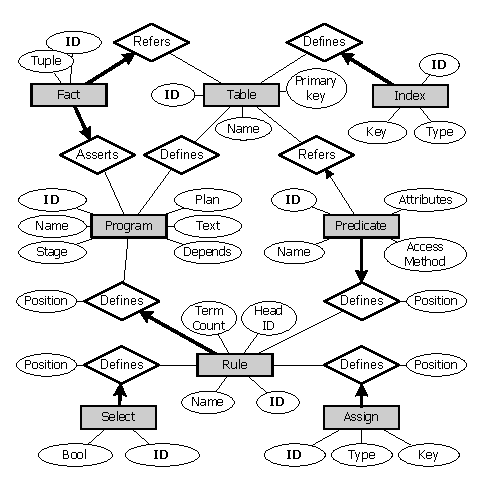
\includegraphics[scale=1.3]{figures/ERDiagram}
\caption{ER Diagram of a query plan in P2. The primary key columns shown in bold.}
\label{ch:evita:fig:p2er}
\end{center}
\end{figure*}

\subsection{Table-izing Optimizer State} 

A typical query optimizer maintains a number of data structures to describe the
contents of a query, and to represent the ongoing state of a query planning
algorithm, including fragments of query plans.  Our first task in designing
Evita Raced was to capture this information in a relational schema.

Figure~\ref{ch:evita:fig:p2er} shows an Entity-Relationship diagram we
developed that captures the properties of an \OVERLOG program, and its
associated P2 dataflow query plans.  We derived the constraints in the diagram
by reviewing the semantic analysis rules enforced in the original P2 compiler;
we discuss a few of them here for illustration.  An \OVERLOG~{\em rule} must
appear in exactly one {\em program}.  A {\em select} term (e.g.,
\ol{f\_contains(X,P2) == false} in Figure~\ref{ch:p2:fig:overlogSP}) is a
Boolean expression over attributes in the predicates of the rule, and must
appear in exactly one {\em rule}.  The diagram indicates that a {\em predicate}
must also appear in a unique {\em rule}, and that it may possibly reference a
single {\em table}.  A predicate that references a table is called a {\em table
predicate} (or a \emph{materialized predicate}), while one that does not is
called an {\em event predicate}.  An {\em index} is defined over exactly one
{\em table}, and a {\em table} defines at least one index (namely the primary
key index, which P2 always constructs).  Some relations may contain {\em facts}
(input tuples) at startup, each of which must belong to a single program and
must reference a single table.

\begin{figure*}
\ssp
\begin{tabular}{|l|l|p{10cm}|} \hline
{\it Name}& {\it Description} & {\it Relevant attributes} \\ \hline\hline
table     & Table definitions & {\bf table\_id}, primary\_key\\ \hline
index     & Index definitions & {\bf index\_id}, {\bf table\_id}, keys, type \\ \hline
fact      & Fact definitions  & {\bf program\_id}, {\bf table\_id}, {\bf id}, tuple\\ \hline
program   & User program description     & {\bf program\_id}, name, stage, text, depends, plan \\ \hline
rule      & Rules appearing in a program   & {\bf program\_id}, {\bf rule\_id}, name,  term\_count, head\_id \\ \hline
predicate & Relational predicates  & {\bf id}, {\bf rule\_id}, table\_id, name, position, access\_method \\ \hline
select    & Selection predicates  & {\bf id}, {\bf rule\_id}, boolean, position \\  \hline
assign    & Variable substitution statements & {\bf id}, {\bf rule\_id}, variable, value, position \\ \hline 
\end{tabular}
\caption{The Metacompiler Catalog: tables defining an \OVERLOG program and dataflow execution plan.
         The primary key columns shown in bold. }
\label{tbl:catalog}
\end{figure*}

The conversion from ER diagram to relational format was a textbook
exercise~\cite{DBTextbook}.  Table~\ref{tbl:catalog} lists the set of relations
that capture the entities mentioned in the ER diagram; we refer to this as the
{\em Metacompiler Catalog}.  We modified P2 to create these tables at system
startup, and they are accessible to any \OVERLOG programs (e.g., optimizations)
subsequently added to the system.
% In addition, there are compiler constraints that cannot be captured by key
% constraints alone.  For instance, a rule must contain exactly one head and
% one event predicate.  Such checks can be performed by integrity constraints
% written into the compiler logic (possibly as \OVERLOG programs).

\subsection{Metacompiler Architecture}
\label{ch:evita:sec:metaarch}
  
\begin{figure*}[htbp]
\centering
\ssp
\begin{tabular}{|l|l|p{10cm}|} \hline
{\it Stage name}& {\it Language} & {\it Description} \\ \hline\hline
StageScheduler & C++ & Coordinates the compilation of stages (Section~\ref{ch:evita:sec:stageschedule}).\\ \hline
Parser    & C++ & Bison based parser. Populates Metacompiler Catalog using program AST.\\ \hline
Planner   & C++ & Generates a dataflow description from the program data contained in the Metacompiler Catalog.\\ \hline
Installer & C++  & Instantiates C++ dataflow objects from a dataflow description. \\ \hline
Delta Rewrite & \OVERLOG  & Converts rules based on materialized tables into an ECA form. \\ \hline
Localization & \OVERLOG   & Rewrites rules containing a distributed joins into a  localized form. \\ \hline
System R & \OVERLOG  & Performs System R dynamic programming optimization on all rules. \\ \hline
Cascades    & \OVERLOG  & Query optimization based on a top-down search strategy. \\  \hline
Magic-sets    & \OVERLOG & Rewrites rules to include magic predicates, which act as
selection predicates for constants contained in query predicates. \\ \hline
Debug print & \OVERLOG & Add special pretty printer predicates, interposed in certain rules. 
The Planner stage translates these printer predicates into dataflow objects that print the tuples
that pass through. \\ \hline
\end{tabular} 
\caption{Primary Evita Raced compiler stages. }
\label{tbl:stages}
\end{figure*}
  

Optimization logic expressed in \OVERLOG is declarative, and Evita Raced
realizes this logic by converting it to a dataflow program to be executed by
the P2 dataflow subsystem, which was described in Section~\ref{ch:p2:sec:p2}.
In this section we describe how Evita Raced represents query optimization
programs as dataflow, and also the way it orchestrates multiple different
optimization programs through the P2 dataflow framework.

An optimizer built using Evita Raced is composed of an extensible number of
{\em stages}, each of which performs some compilation task on the input
program.  Table~\ref{tbl:stages} describes the primary compiler stages packaged
with the Evita Raced framework.  An Evita Raced stage can be written as a
dataflow program of one or more P2 elements in C++, which are then compiled
into the P2 binary; this is how we implement certain base stages required for
bootstrapping, further described in Section~\ref{ch:evita:sec:bootstrap}.  However,
the power of Evita Raced comes from its support for stages written in \OVERLOG,
which, in addition to being compactly expressed in a high-level language, can
be loaded into a running P2 installation at any time.

A stage programmer registers a new stage with Evita Raced by inserting a tuple
into the \ol{program} relation.  This tuple contains a unique identifier
($program\_id$), a name ($name$), a list of stage dependencies ($depends$), and
the program text ($text$).  Because the \ol{program} relation is used to convey
partial compilation results from stage to stage as well, \ol{program} tuples
also contain attributes for the name of the compiler stage currently operating
on the program ($stage$), and the final physical plan ($plan$), though these
attributes are empty when the programmer first creates the tuple.
Section~\ref{ch:evita:sec:stageschedule} describes the $depends$ attribute, and
its use in the installation of new stages.  The $plan$ attribute pertains to
the physical planner stage, which is described in
Section~\ref{ch:evita:sec:planner}.  We next describe the interfaces to an
Evita Raced compiler stage, after which we discuss the way that multiple such
stages are coordinated.

\subsubsection{The Stage API}

At base, an Evita Raced stage can be thought of as a stream query that listens
for a tuple to arrive on an event stream called \ol{<stage>::programEvent},
where \ol{<stage>} is the name of the stage.  The \ol{<stage>::programEvent}
table contains all the attributes mentioned in the \ol{program} table.  When
such a tuple arrives, the queries that make up that stage execute, typically by
modifying catalog tables in some way.  When a stage competes it inserts a new
\ol{program} tuple, containing the name of the stage in the $stage$ attribute,
into the program table.

To represent this behavior in a stage written in \OVERLOG, a relatively simple
template can be followed.  An \OVERLOG stage must have at least one rule body
containing the \ol{<stage>::programEvent} predicate.  This represents the
ability of the stage to react to new programs arriving at the system.  In
addition, the stage must have at least one rule that inserts a \ol{program}
tuple into the \ol{program} table to signal stage completion.

\subsubsection{Stage Scheduling}
\label{ch:evita:sec:stageschedule}

In many cases, optimization stages need to be ordered in a particular way for
compilation to succeed.  For example, a {\em Parser} stage must run before any
other stages, in order to populate the Metacompiler Catalogs.  The {\em
Planner} must follow any stages written in \OVERLOG, since it is responsible
for translating the relational representation of a query into a dataflow
representation.  And finally, the {\em Installer} stage must follow the {\em
Planner}, since it instantiates dataflow specifications as P2 C++ elements, and
installs them into the P2 runtime.  We will see other specific precedence
constraints in Section~\ref{ch:evita:sec:stages}.

A natural way to achieve such an ordering would be to ``wire up'' stages
explicitly so that predecessor stages directly produce
\ol{<stage>::programEvent} tuples for their successors, in an explicit chain of
stages.  However, it is awkward to modify such an explicit dataflow
configuration upon registration of new stages or precedence constraints.
Instead, Evita Raced captures precedence constraints as {\em data} within a
materialized relation called \ol{StageLattice}, which represents an arbitrary
partial order (i.e., an acyclic binary relation) among stages; this partial
order is intended to be a lattice, with the {\em Parser} as the source, and the
dataflow {\em Installer} as the sink.  
 
To achieve the dataflow connections among stages, the built-in {\em
StageScheduler} component (itself a stage) listens for updates to the
\ol{program} table, indicating the arrival of a new \OVERLOG program or the
completion of a compiler stage for an on-going program compilation.  The {\em
StageScheduler} is responsible for shepherding compilation stage execution
according to the \ol{StageLattice}.  Given a \ol{program} update, it ''joins with`` the
lattice to identify a next stage that can be invoked, and generates the
\ol{<stage>::programEvent} tuple that will start that stage; the contents of
the tuple are the same as those of the updated \ol{program} tuple.

\begin{figure*}[htbp]
\begin{center}
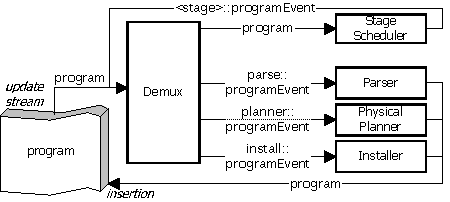
\includegraphics[scale=1.5]{figures/DefaultCompiler}
\ssp
\caption{The Evita Raced (cyclic) dataflow architecture, containing only the default compilation stages.}
\label{ch:evita:fig:basecompiler}
\end{center}
\end{figure*}

The {\em StageScheduler} and any compilation stages (whether built-in or
runtime-installed) are interconnected via the simple dataflow illustrated in
Figure~\ref{ch:evita:fig:basecompiler}.  This is the same dataflow architecture
used throughout the {\em Declarative Networking} project.  As described in
Section~\ref{} (and~\cite{p2:sosp}), it consists of a C++ ``demultiplexer''
that routes tuples from its input (on the left) to individual event handlers
listening for particular tuple names (the arrows leaving the Demux element in
the figure contain the name of the tuple for which the four components to the
right listen).  The Evita Raced framework simply adds the its ''default
stages`` to the bootstrap routine of the P2 system.

Consider the simplicity of how the Evita Raced framework coexists with the P2
dataflow architecture.  To install a new (\OVERLOG) compilation stage into the
runtime, the Installer stage (Section~\ref{ch:evita:sec:installer}) simply extends
the {\em Demux} element to include a port for \ol{<stage>::programEvent}
tuples, routing them to the respective rule(s) of a given stage's \OVERLOG
program. The \ol{StageLattice} relation is also updated (e.g., through fact tuples
in the \OVERLOG stage program) to include its position in the compilation pipeline.
This completes the installation process, after which the \OVERLOG stage need only 
follow a simple protocol for when and how it should execute. 

The protocol to stage execution indicates when it should start (after receiving
a \ol{<stage>::programEvent} tuple) and what it must do on completion.  When a
stage completes, the only requirement is to update the \ol{program} table to
indicate this fact.  The {\em StageScheduler} receives all such updates to the
\ol{program} table -- see Figure~\ref{ch:evita:fig:basecompiler}, the {\em
Demux} \ol{program} tuple port into the {\em StageScheduler} -- and uses the
value of the \ol{program} $depends$ attribute along with the \ol{StageLattice}
relation to determine the next stage.  This completes the full compilation
process in Evita Raced of an \OVERLOG program, from the {\em Parser} stage to the {\em
Installer} stage, and any other stages along the way.

To sum up, the life cycle of a program compilation starts when a user submits a
\ol{program} tuple to the system with a \ol{null} stage attribute.  The
StageScheduler receives that \ol{program} tuple and generates a
\ol{parse::programEvent} tuple (the Parser being the source stage in the
lattice), which is routed by the Demux element to the Parser stage.  When the
Parser is done, it updates that \ol{program} tuple in the corresponding table,
changing the tuple's attribute to ``Parser.'' The StageScheduler receives the
\ol{program} tuple, and routes a \ol{planner::programEvent} to the Demux and
eventually the Physical Planner, which goes round the loop again to the
Installer.  Finally, once the Installer is done and notifies the StageScheduler
via a \ol{program} tuple with the \ol{stage} attribute set to ``Installer,''
the StageScheduler concludes the compilation process.  If the \OVERLOG program
being parsed is itself a new compilation stage, then after installation, the
scheduler updates the stage lattice.


\subsection{Compiler Bootstrapping}
\label{ch:evita:sec:bootstrap}

This section drills down on the stages that make up the baseline Evita Raced
compiler that is now part of P2's bootstrap routine.  As in many
metaprogramming settings, this is done by writing a small bootstrap component
in a lower-level language.  Evita Raced is initialized by a small C++ library
that constructs the cyclic dataflow of Figure~\ref{ch:evita:fig:basecompiler},
including the three default stages shown, which are themselves written in C++.
The entire bootstrap, including the stages is around {\bf 400} lines of C++.
The bootstrap compiler is sufficient to compile simplified \OVERLOG programs
(local rules only, no optimizations) into operational P2 dataflows.  We next
describe each of the three bootstrap stages (Parser, Planner, and Installer) in
a bit more detail, since they form the core foundation of the Evita Raced
framework.

% \jmh{This paragraph was saved from a conflict with Tyson's checkin.  Joe will merge it in Tuesday night.
% The {\em stage scheduler} is a dataflow element that is responsible for providing the inputs to a 
% stage and processing any outputs from a stage. The input to a stage module is a tuple containing the 
% identifier of the program that it is responsible for
% processing. When the stage completes its task is will insert a new program tuple into
% the \ol{program} table with an updated $state$ attribute value that indicates (to the scheduler) the completion 
% of the stage operation on the input program. The program insertion triggers a new
% \ol{programEvent} tuple that is again directed to the stage scheduler, and the process repeats with
% the next scheduled stage in the compilation order. Stage execution order is determined by
% a relation of stage dependencies. The stage scheduler schedules
% a stage based on the dependency graph relation installed by the bootstrap process and the current 
% value of the $state$ attribute in the program tuple. The process completes when the program $state$ 
% attribute reaches stage that no other stage depends on.
% }


% \subsubsection{Default Query Compilation}
% 
% Figure~\ref{ch:evita:fig:basecompiler} shows a dataflow perspective of our default
% metacompiler. A user submits a new program to the system by inserting a tuple into the \ol{program} table.
% The program tuple contains initial values for all the attributes in the program table (see Table~\ref{tbl:tables}). 
% A program table insertion triggers a \ol{programEvent} event tuple that contains the program 
% identifier attribute value.  The "Demux" dataflow element routes the \ol{programEvent} tuple to the
% stage scheduler element, which determines the order in which a stages execute on the input
% program. 
% \petros{The job of the scheduler is a bit nebulous. Is there something
% you can say here to make clear what that does?}
% 
% 
% The input to a stage module is a tuple containing the identifier of the program that it is responsible for
% processing. When the stage completes its task is will insert a new program tuple into
% the \ol{program} table with an updated $State$ attribute value that indicates (to the scheduler) the completion 
% of the stage operation on the input program. The program insertion triggers a new
% \ol{programEvent} tuple that is directed to the stage scheduler, and the process repeats with
% the next scheduled stage in the compilation order. Stage execution order is determined by
% a relation of stage dependencies. The stage scheduler schedules
% a stage based on the dependency graph and the current value of the $State$ attribute in the program tuple. 
% The process completes when the program $State$ attribute reaches stage that no further stage depend on.
% 

\subsubsection{Parser}

The Parser passes the program text it receives in the \ol{programEvent}
through a traditional lexer/parser library specified using
flex~\cite{flexUrl} and bison\cite{bisonUrl}; this library code returns
a standard {\em abstract syntax tree} representation of the text.
Assuming the Parser does not raise an exception due to a syntax error,
it walks the abstract syntax tree, generating Metacompiler Catalog
tuples for each of the semantic elements of the tree. In addition to
recognizing the different terms of each rule, the parser also annotates
each term with its position in the given program.  By convention, the
first term of a rule body is the event predicate of the rule, if one
exists.  By the same convention, the term in the last position for a
rule is the head predicate.



\subsubsection{Physical Planner}
\label{ch:evita:sec:planner}

The Physical Planner stage is responsible for doing a na\"{i}ve translation of
Metacompiler Catalog tuples (i.e., a parsed \OVERLOG program) into a dataflow
program.  It essentially takes each rule and deterministically translates it
into a dataflow graph language, based on the positions of terms in the rule.

More specifically, for each rule the Planner considers each term (predicate,
selection or assignment) in order of position attribute.  The predicate
representing the event stream is always planned first, and registers a listener
in the Demux element (recall Figure~\ref{ch:evita:fig:basecompiler}).  The
terms following the event stream are translated, left-to-right, into a C++
dataflow in the same way that the original P2 system did, so we do not address
them further here.

We do mention three specific details.  First, whereas the original P2 system
translated a logical query plan directly to a software dataflow structure in
C++, we have chosen to create an intermediate, textual representation of the
dataflow.  This representation is in a language akin to the Click router's
dataflow language, but we omit its details here.

Second, unlike the original P2 system, we have introduced a number of access
methods for in-memory tables.  Our \ol{predicate} relation contains the access
method as one of the attributes, and we have modified the P2 physical planner
to choose the appropriate dataflow element that implements the given access
method.

%% Those are naturally introduced to the P2 physical planner
%% machinery and otherwise
%% creates
%% a listening port in the P2 {\em Demux} on the event stream name. The predicates mentioned in the rule that
%% do not represent the event stream represent lookup operations (joins) on the referenced base relation.
%% A join operator is planned for a predicate by taking the input stream and schema and joining 
%% it - using the $access\_method$ given by the \ol{predicate} tuple - with a base relation producing a new tuple 
%% stream with the join schema. 
%% A selection term plans a filter operator that applies the $boolean$ attribute value to the input 
%% stream and passes only tuples that satisfy this expression to the output stream. \jmh{Again the "plans an operators that does X" doesn't mean much to me.}An assignment term 
%% plans a assignment operator that uses the input stream to evaluate the $value$ attribute (in the \ol{Assign}
%% tuple) to an atomic value. If the input stream contains an attribute named by $variable$ 
%% (in the \ol{Assign} tuple) then the value of that attribute is substituted in the input
%% stream, otherwise a new attribute is added to the input schema with the given value 
%% in the output stream. After all rule body terms have been planned, the planner adds a projection operator
%% that projects the output tuple stream onto the head predicate.

% generates a physical plan for each rule in a program. The execution order of a physical plan in 
% P2 is a leaf-to-root path, with the leaf corresponding to the event predicate and the root being the head 
% predicate. All predicates that lie in between the leaf and the root path are joined against the respective 
% base relation according to the access method given by the predicate tuple. 
% \petros{I would go as far as saying that the physical plan you derive is
% expressed in an operator language reminiscent of the Click
% language. Since we concentrate on logical plan manipulations here we
% don't go into details. The important thing to point out is that whatever
% you do is not tied to a particular runtime; one could take this physical
% plan and install it on a different runtime that isn't our dataflow but
% something else.}

% The initial operator is always the event predicate and it determines when the rule should fire. 
% If the rule does not contain an event predicate then a delta rewrite must be preformed on the rule. 
% The delta rewrite converts the original rule into a set of new rules
% that trigger whenever a side affect\petros{``side affect'' should be
%   ``side effect'' everywhere.} 
% occurs on a table predicate mentioned in the original rule. The delta rewrite is presented 
% in~\cite{boonSigmod}, and we fully adopt this rewrite in our metacompiler. The position attribute 
% defined by each predicate tuple determines the position of the corresponding physical operator in 
% the physical plan. Select and assign operators are also planned at the position indicated by the 
% respective table tuple.

Third, the Planner only understands rules that are in the
event-condition-action (ECA) form. An \OVERLOG rule may have no event
predicate (e.g., ``\ol{table1 :- table2, table3.}'').  A {\em delta rewrite}
(from Loo, et al.~\cite{loo-sigmod06}) is used to convert such rules in an ECA
form (E.g., ``\ol{table1 :- delta\_table2, table3.}'' and ``\ol{table1 :-
table2, delta\_table3.}''.) As in~\cite{loo-sigmod06} \ol{delta\_table} denotes
a stream conveying insertions, deletions, or timeout refreshes to tuples of the
table \ol{table}.  We could have chosen to do this directly in the Planner, but
instead we built it as an \OVERLOG stage.  This decision had an
important consequence; we could only use rules that contained an explicit event
predicate.  Furthermore, any \OVERLOG stage that contained rules with no
explicit event predicate depended on this compilation stage.  The delta rewrite
\OVERLOG stage consists of a mere $6$ rules ($25$ lines of code), and is
usually the first \OVERLOG stage to be compiled into the runtime.
 

\subsubsection{Plan Installer}
\label{ch:evita:sec:installer}

Given the output of the Physical Planner in the dataflow specification
language, what remains is to parse the
textual representation of the dataflow,  construct the
corresponding C++ elements, and ``wire them up'' accordingly. We have
implemented this 
``physical plan compiler'' in C++, and housed it within the
Installer stage.  Once these elements and their connections are
instantiated, the Plan Installer stage stitches them into the P2
runtime's overall dataflow graph, as described in~\cite{p2:sosp}.
As noted in~\ref{ch:evita:sec:metaarch}, this infrastructure made it easy for us to extend P2 with the ability to modify its dataflow graph at runtime,
a feature not available in the released system. 
% Since our focus here
% is on plan optimization, we omit the engineering
% details of that contribution.
% 


\subsection{Discussion}

The metacompilation approach of Evita Raced led us to naturally design the
system extensibility around issues of data storage and dataflow, rather than
library loading and control flow modifications.  While rule-based systems are
usually intended to be easier to extend than a procedural system, the internal
implementation of Evita Raced is especially elegant, due to our thorough
embrace of the native dataflow infrastructure, which we use both to execute
optimization code, and orchestrate stages via precedence tables and the
StageScheduler cycle.  The result of this design is that even a major addition
to the Evita Raced compiler entails very minimal modification to the runtime
state: only the addition of a pair of dataflow edges to connect up the new
stage, and the insertion of precedence tuples in a single table.  Beyond the
StageScheduler and the three bootstrap stages, no additional extensibility code
was added to P2 to support Evita Raced.

Despite its simplicity, Evita Raced is flexible enough that other researchers
have used it to enhance P2 with support for new languages at both its input and
output.  First, by extending the Parser element and registering some \OVERLOG
rules, Abadi and Loo were able to get P2 to optimize and rewrite programs
written in a new language, which extends \OVERLOG with the ability to attest to
the provenance of data in a manner similar to that of~\cite{abadi-netdb07}.
Second, Chu, et al. were able to use Evita Raced to cross-compile \OVERLOG programs
into dataflow specifications that execute on the DSN platform, a declarative
networking system that runs on wireless sensor nodes~\cite{chu-sensys07}.
% In Section~\ref{ch:evita:sec:dsn} we present results from running Evita Raced
% plans in DSN on Berkeley Mote hardware.


\section{Query Compilation Stages}
\label{ch:evita:sec:stages}

% \jmh{This paragraph is thoroughly redundant with hte previous section and can be chopped.  However, it'd be nice to have some kinda warmup text here.}
% A compilation stage written in the P2 query language is dynamically installed into the compiler 
% at runtime, using the same compilation path taken by any \OVERLOG program. The stage programmer 
% inserts a program tuple containing the text of an \OVERLOG program. The programmer also specifies, 
% in the {\em depends} attribute of the program tuple, a single stage that should execute immediately 
% before the installed stage.  After the insertion into the program table, the stage scheduler receives 
% the \ol{programEvent} tuple, which it uses to access the program tuple. The program is processed
% by the stages that appear in the current dependency graph relation. The stages treat the program 
% no differently than any other program. Once the program has been successfully installed, the stage 
% scheduler will then notice that the $depends$ attribute of the program tuple contains a 
% reference to a preexisting stage. 
% The dependency reference informs the stage scheduler that installed program represents a new stage, and 
% that it should update the dependency relation accordingly. After performing the update to the dependency
% relation, the new stage will be included in the compilation process of future input programs. 

Having described the Evita Raced infrastructure, we now turn to the issue of
specifying query optimizations in \OVERLOG.  In this section we describe three
of the compiler stages we have developed for Evita Raced.
Section~\ref{ch:evita:sec:systemr} discusses a dynamic programming optimizer
stage akin to that of System R.  We present, in
Section~\ref{ch:evita:sec:cascades}, an optimization that performs a top-down
search strategy, which is modeled after the Cascades optimizer.
Section~\ref{ch:evita:sec:magic} describes a stage that performs magic-sets
rewrite on recursive \OVERLOG programs.  Finally,
Section~\ref{ch:evita:sec:localization} describes our reimplementation in Evita
Raced of the localization rewrite from Loo et al.~\cite{loo-sigmod06}.

\subsection{System R Optimization}
\label{ch:evita:sec:systemr}

\begin{figure*}
\ssp
\centering
\begin{boxedminipage}{\linewidth}
  {\bf def} optimizer($Q$)
    \begin{algorithmic}[1]
      	\STATE /* Base case: access methods to relations in Q */
  	\FORALL{base relations $R \in Q$}
		\STATE Find all access methods to $R$ and store in $AM$
		\STATE Include index scans iff there exists sargable predicates 
  	\ENDFOR
	\STATE
  	\FORALL{$p \in AM$}
		\IF{$p$ is the cheapest unordered access method \OR 
		    $p$ is the cheapest access method for some "interesting order"}
			\STATE $plans[1] = plans[1] \bigcup p$ 
		\ENDIF
 	\ENDFOR
	\STATE
	\STATE $bp$ = bestplan($|Q|$) /* Get best plans for query Q */
	\IF{$Q$ contains a GROUP BY or ORDER BY}
	 	\STATE $cp$ = cheapest plan $p \in bp$ w.r.t. relevant interesting order 
		\IF{$cp == null$}
			\STATE $cp$ = cheapest overall plan $p \in bp$ + sort operator
		\ENDIF
		\RETURN $cp$
	\ELSE
	 	\RETURN cheapest overall plan $p \in cp$ /* irrespective of ``interesting orders'' */ 
	\ENDIF
    \end{algorithmic}
  {\bf end} \\
  \\
  {\bf def} bestplan(n)
    \begin{algorithmic}[1]
  	\IF{$plans[n] = \emptyset$}
		\FORALL{$p_1 \in plans[1]$} 
			\STATE $P_{n-1}$ = bestplan(n -1)
			\FORALL{$p_{n-1} \in P_{n - 1}$}
			\STATE /* if $p_1$ and $p_{n-1}$ have non-overlapping query predicates */
				\IF{$p_1 \bigcap p_{n-1} = \emptyset$}
					\STATE $plans[n] = plans[n] \bigcup$ all (left-outer) join methods for $p_1$ and $p_{n-1}$
				\ENDIF
			\ENDFOR
		\ENDFOR
		\STATE
		\FORALL{$p \in plans[n]$}
			\IF{$p$ is not the cheapest unordered plan among its equivalent plans \OR
			    $p$ is not the cheapest ``interesting ordered'' plan among its equivalent plans}
				\STATE delete $p$ from $plans[n]$
			\ENDIF
		\ENDFOR
	\ENDIF
	\RETURN plans[n]
      \end{algorithmic}
    {\bf end}
\end{boxedminipage}
\caption{\label{ch:evita:fig:systemr}System R optimizer algorithm.}
\end{figure*}

The System R optimizer paper by Selinger, et al.  is the canonical textbook
framework for database query optimization~\cite{selinger}.  The paper laid out
for the first time the notion that query optimization can be decomposed into
two basic parts: query plan cost estimation and plan enumeration.  While this
algorithm is traditionally implemented inside the heart of a database system
via a traditional procedural programming language, both of these tasks are
naturally specified in a declarative query language.  To perform cost
estimation, System~R requires data statistics like relation cardinalities and
index selectivities; \OVERLOG is a fitting language to collect these
statistics, especially in a distributed fashion over all relation partitions.

Our focus in this section is on the basic dynamic programming algorithm for the
state-space enumeration at the heart of the System R optimizer.
Figure~\ref{ch:evita:fig:systemr} gives a (simplified) sketch of this
algorithm.  It enumerates query plans for increasingly-large subgoals of the
query optimizer.  It fills in a dynamic programming table (e.g., $plans$ in
Figure~\ref{ch:evita:fig:systemr}) with plans that cover a given number of
(relational algebra) predicates that appear in the query.  The dynamic
programming task is to fill in this table with the lowest-estimated-cost query
plan among all plans producing an {\em equivalent} output relation (i.e., plans
composed of the same terms).  The \ol{bestplan} procedure in
Figure~\ref{ch:evita:fig:systemr} captures the essence of generating and
choosing optimal plans with a given number of predicates.

In the System R optimizer, the {\em principle of optimality} is assumed to hold: the
lowest-cost solution to some plan will be built from the optimal solutions to
subplans.  Thus dynamic programming can proceed in ``bottom-up'' fashion.  In a
given program $P$ to be optimized, each rule's event predicate is the
``outermost,'' streaming relation in a query plan for the rule.  For a given
rule $r \in P$, the optimizer generates plans of size $k$ terms by appending a
single (thus unused) term from the rule body to the optimal plan of size $k-1$
terms, as shown in the first loop of \ol{bestplan} in Figure~\ref{ch:evita:fig:systemr}.
There are many additional details that we have chosen to gloss over in the
pseudocode.  

For instance, avoid combining a k-way plan with a 1-way plan if there is no
join predicate between them, unless all predicates have been used up (i.e.,
postpone Cartesian products).  We handle this in our \OVERLOG rules by ensuring
the cost of such an option is greater than any other option that includes join
predicates.  We now turn to describe the \OVERLOG rules for plan generation and
conclude with the rules for best plan selection.

\subsubsection{Plan Generation}
\label{ch:evita:sec:plangen}

\begin{figure*}
\ssp
\centering
\begin{boxedminipage}{\linewidth}
pg1 {\bf plan}(@A, Pid, Rid, PlanID, SubPlanID, Type, TypeID, \\
\datalogspace \xspace \xspace Plan, Schema, Card, Cost, Pos, AM, Sort) :- \\
\datalogspace {\bf systemr::programEvent}(@A, Pid, \_, \_, \_, \_, \_, \_),\\
\datalogspace {\bf predicate}(@A, PredID, Rid, \_, \_, \_, \_, Schema, Pos, \_, \_),\\
\datalogspace Pos == $1$,\\
\datalogspace PlanID := {\em f\_idgen()}, SubPlanID := $null$,\\
\datalogspace Type := "Predicate", TypeID := PredID,\\
\datalogspace Plan := {\em f\_cons}(PredID, $null$),\\
\datalogspace Card := $1$, Cost := $1$,\\
\datalogspace AM := "STREAM", Sort := $null$.
\end{boxedminipage}
\caption{\label{ch:evita:fig:planseed}Plan seed rule.}
\end{figure*}

Figure~\ref{ch:evita:fig:systemr} presents the System R algorithm for plan
generation in two phases.  The first is generating all access methods for a
given relation mentioned in the query (e.g., in the ``from'' clause).
Subsequent to that, a second phase enumerates all possible join orders and
methods.  Recall in Section ? that P2 converts a rule into an
event-condition-action (ECA) form, where the event predicate represents a
stream of tuples from the table reference.  As a consequence of this dataflow
design, our first phase simply generates a plan that listens for such event
tuples.  Extending this rule to consider access methods would entail adding a
predicate that references all access methods to a given relation.

Figure~\ref{ch:evita:fig:planseed} shows the optimizer rule that creates the
initial plan for each rule from the event predicate.  The \ol{plan} tuple
contains a query plan for a given rule, and the plan's \ol{size} reflects the
number of term identifiers in the $Plan$ attribute (i.e., the number of leaves
in the plan tree).  The optimizer listens on the \ol{programEvent} event stream
in rule \ol{pg1}, which initiates the optimization process.  The
\ol{programEvent} tuple is subsequently joined with the \ol{rule} table along
the $Pid$ (program identifier) attribute to obtain the set of rules defined in
the input program.  The resulting set of rule tuples are each joined with the
\ol{predicate} table along the $Rid$ (rule identifier) attribute.  The result
of this join produces a tuple for each predicate term defined by a given rule.
The predicate term assigned to position~$1$ ($Pos == 1$) is by convention the
event predicate term.  For each event \ol{predicate} tuple in each rule of the
input program, rule \ol{pg1} adds a new plan to the \ol{plan} table.  The
$Plan$ attribute represents the initial plan list, starting with the term
identifier ($PredID$) that identifies streaming predicates.  Plan generation
proceeds by appending term identifiers to this list when constructing new plans
from optimal subplans.

The \OVERLOG optimizer defines a set of plan generation rules that together
perform the induction step of the dynamic program.  Each rule extends a best
plan of $k$ terms with a $(k+1)^{st}$, thus far unused term from the rule body.
If the new term considered is a table predicate, then the new plan
annotated with an appropriate join method, which takes the optimal subplan and
``joins it'' with the predicate table.  The join methods supported by P2
include scanned and index-nested-loop-join, as well as merge-join.  A plan
tuple also carries with it an associated cost, which only considers CPU costs
since all P2 relations reside in memory.  We now turn to the description of the
rules that generate plans for nested-loop-join, index nested-loop-join, and
sort-merge join methods.

\begin{figure*}
\ssp
\centering
\begin{boxedminipage}{\linewidth}
\linenumbers
pg2 {\bf plan}(@A, Pid, Rid, {\em f\_idgen()}, PlanID, "Predicate", PredID, \\
\datalogspace \xspace Plan, Schema, Card, Cost, OuterPos+$1$, JM, $null$) :-\\
\datalogspace {\bf bestPlan}(@A, Pid, Rid, PlanID),\\
\datalogspace {\bf plan}(@A, Pid, Rid, PlanID, \_, \_, \_, OuterPlan, \\
\datalogspace \datalogspace OuterSchema, OuterCard, OuterCost, OuterPos, \_, \_),  \\   
\datalogspace {\bf predicate}(@A, PredID, Rid, \_, \_, Tid, \_, PredSchema, PredPos, \_, \_),\\
\datalogspace {\bf rule}(@A, Rid, Pid, \_, \_, \_, \_, TermCount), \\
\datalogspace $PredPos < TermCount$,\\
\datalogspace {\bf table}(@A, Tid, \_, \_, \_, \_, TCard, \_),\\
\datalogspace {\em f\_contains}(PredID, OuterPlan) == $false$,\\
\datalogspace Card := OuterCard * TCard / $10$,\\
\datalogspace Cost := OuterCost + (OuterCard * TCard),\\
\datalogspace JM := NESTED\_LOOP, \\
\datalogspace Plan := {\em f\_cons}(PredID, OuterPlan), \\
\datalogspace Schema := {\em f\_merge}(OuterSchema, PredSchema).\\
\end{boxedminipage}
\caption{\label{ch:evita:fig:plangen1}nested-loop join method.}
\end{figure*}

Any table predicate appearing in a rule body is given a nested-loop-join plan,
shown by rule~\ol{pg2} in Figure~\ref{ch:evita:fig:plangen1}.  The rule is
triggered on an update to the \ol{bestPlan} relation (described in
Section~\ref{}), which contains the plan identifier ($PlanID$) used to select
the reference plan in the \ol{plan} relation.  Each plan tuple contains a list
of the predicate identifiers that already appear in it.  This list is
referenced by the $OuterPlan$ variable in the \ol{plan} predicate of
rule~\ol{pg2}.

The next step is to extend the \ol{plan} tuple with a ``new'' table predicate,
which is done by joining with the \ol{predicate} relation along the same rule
identifier ($Rid$).  The result of this join operation produces all predicates
mentioned in the rule.  To get only the table predicates we join with the
\ol{table} predicate.  The selection predicate $PredPos < TermCount$ ensures that
we do not consider the rule head predicate (last in the rule's terms by
convention).  The function $f\_contains$ tests for containment of the predicate
in the subplan (outer plan).  The tuples that meet the constraints imposed thus
far represent new table predicates that can be used to extend the optimal plan.
We need only assign annotate the new (projected) plan tuple with a join method
(NESTED\_LOOP), associated cost (based on cardinality estimates), a new
predicate list (see $Plan$ variable), and a new schema (see $Schema$ variable).

\begin{figure*}
\ssp
\centering
\begin{boxedminipage}{\linewidth}
pg3 {\bf plan}(@A, ...) :-\\
\datalogspace {\bf bestPlan}(@A, Pid, Rid, PlanID),\\
\datalogspace {\bf plan}(@A, Pid, Rid, PlanID, \_, \_, \_, OuterPlan, \\
\datalogspace \datalogspace OuterSchema, OuterCard, OuterCost, OuterPos, \_, \_),  \\   
\datalogspace {\bf predicate}(@A, PredID, Rid, \_, \_, Tid, \_, PredSchema, PredPos, \_, \_),\\
\datalogspace {\bf rule}(@A, Rid, Pid, \_, \_, \_, \_, TermCount), \\
\datalogspace $PredPos < TermCount$,\\
\datalogspace {\bf table}(@A, Tid, \_, \_, \_, \_, TCard, \_),\\
\datalogspace {\bf index}(@A, Iid, Tid, Key, Type, Selectivity),\\
\datalogspace {\em f\_contains}(PredID, OuterPlan) == $false$,\\
\datalogspace {\em f\_indexMatch}(OuterSchema, PredSchema, Key),\\
\datalogspace Card   := OuterCard * (Selectivity * TCard),\\
\datalogspace Cost   := OuterCost + Card,\\
\datalogspace AM := {\em f\_cons}(Type, Iid),\\
\datalogspace ...
\end{boxedminipage}
\caption{\label{ch:evita:fig:plangen2}index-nested-loop join method (diff from Figure~\ref{ch:evita:fig:plangen1}).}
\end{figure*}

An index-nested-loop join plan is generated by rule \ol{pg3} in
Figure~\ref{ch:evita:fig:plangen2}.  Like rule~\ol{pg2}, it joins the
\ol{bestPlan}, \ol{plan}, \ol{predicate}, and \ol{table} predicates to
get all table predicates referenced by the target rule.  That result is
subsequently joined with the (additional) \ol{index} predicate, which adds
index information to the result tuples.  The function {\em f\_indexMatch} tests
if the index can be used to perform the join using attributes from the best
plan schema ($OuterSchema$) and attributes from the predicate table
($PredSchema$).  Any tuple results from this plan are assigned cardinality and
cost estimates based on some cost function, which uses the additional index
selectivity information given by the $Selectivity$ \ol{index} predicate
attribute.  We also support range predicates in our index-nested-loop join
plans but do not discuss them in detail as they are quite similar to the
nested-loop cases above.

A merge-join performs a join of a plan with a table predicate mentioned in the
rule body along some sorting attribute.  The tuple set from the outer plan and
the predicate table must be ordered by the sorting attribute.  The output of a
merge-join operation preserves the sorting attribute order.  Therefore, the
\ol{plan} predicate generated by the merge-join rule includes the sorting
attribute in the value of the $Sort$ \ol{plan} predicate.  We note that the
$Sort$ attribute in the \ol{table} plan table identifies the sorting attribute
of the table.  A $null$ valued $Sort$ attribute, in either the outer relation
\ol{plan} predicate or the inner relation \ol{table} predicate, means that the
relation is not known to be ordered, and must be presorted prior to the
merge-join operator.  The cost of a merge-join operator depends on need to
presort either relation.

\subsubsection{Best plan selection}
\label{ch:evita:sec:bestplan}

\begin{figure*}
\ssp
\centering
\begin{boxedminipage}{\linewidth}
bp1 {\bf bestCostPlan}(@A, Pid, Rid, Plan, Sort, {\small \bf a\_min}<Cost>) :- \\
\datalogspace {\bf plan}(@A, Pid, Rid, \_, \_, \_, \_, Plan, \_, \_, Cost, \_, \_, Sort, \_). \\
\\            
bp2 {\bf bestPlan}(@A, Pid, Rid, PlanID, Plan2, Cost) :- \\
\datalogspace {\bf bestCostPlan}(@A, Pid, Rid, Plan1, Sort, Cost), \\
\datalogspace {\bf plan}(@A, Pid, Rid, PlanID, \_, \_, \_, Plan2, \_, \_, Cost, \_, \_, Sort, \_), \\
\datalogspace Sort == $null$.\\
\\
bp3 {\bf interestingOrder}(@A, Pid, Rid, PlanID) :- \\
\datalogspace {\bf plan}(@A, Pid, Rid, PlanID, \_, \_, \_, Plan, \_, \_, Cost, \_, \_, Sort, \_), \\
\datalogspace {\bf rule}(@A, Rid, Pid, \_, \_, \_, \_, TermCount), \\
\datalogspace {\bf predicate}(@A, PredID, Rid, \_, \_, Tid, \_, PredSchema, PredPos, \_, \_),\\
\datalogspace {\bf select}(@A, Sid, Rid, Pred, \_, \_), \\
\datalogspace // participates in a later join OR is a prefix of a grouping attribute \\ 
\datalogspace ({\em f\_contains}(PredID, Plan) ==  $false$ \&\& Pred.contains(Sort)) $||$ \\
\datalogspace (PredPos == TermCount \&\& PredSchema.isGroupingAttribute(Sort)). \\
\\
bp4 {\bf bestPlan}(@A, Pid, Rid, PlanID, Plan2, Cost) :- \\
\datalogspace {\bf bestCostPlan}(@A, Pid, Rid, Plan1, Sort1, Cost), \\
\datalogspace {\bf plan}(@A, Pid, Rid, PlanID, \_, \_, \_, Plan2, \_, \_, Cost, \_, \_, Sort2, \_), \\
\datalogspace {\bf interestingOrder}(@A, Pid, Rid, PlanID), \\
\datalogspace {\em f\_setequals}(Plan1, Plan2), Sort1 == Sort2.\\
\\            
\end{boxedminipage}
\caption{\label{ch:evita:fig:bestplan}Best plan selection.}
\end{figure*}

Figure~\ref{ch:evita:fig:bestplan} shows the rules that select the best plan
from a set of equivalent plans, in terms of the output result set and the
ordering properties of the result set.  The \ol{bestCostPlan} predicate of
rule~\ol{bp1} contains the plan with the minimum cost from the set of
equivalent plans.  This aggregation query groups along the program identifier,
rule identifier, plan list~\footnote{The plan lists are actually sets of
predicate identifiers, which forces the grouping operator to use a set
comparison method to test for equivalence.}, and sort attribute.  The inclusion
of the sort attribute in the group condition {\emph enables} the handling of
what Selinger calls ``interesting orders''~\cite{selinger}, along with optimal
subplans.

The remain rules deal with populating the \ol{bestPlan} table with the optimal
unordered and interestingly ordered plans.  Rule~\ol{bp2} selects the best
unordered plan (no ordering attributes $Sort == null$).  An interesting order
is determined in rule~\ol{bp3} by considering the Sort attribute of a plan with
new join predicates and grouping attributes.  The new join predicates are
simply those table predicates not already mentioned in the plan list.  The
grouping attributes are given by the head predicate (in the last position)
through a special method that returns true iff there is a grouping and the Sort
variable references a prefix of the grouping attributes.  This completes our
consideration of interesting orders, since \OVERLOG does not have a notion of
an "order by" clause.  Rule~\ol{bp4} uses the \ol{interestingOrder} predicate
to choose the optimal plan with the given order.
 
\subsubsection{Improving Selectivity Estimation}

For equality selection predications, our System R rules above support selectivity
estimates using a uniform distribution estimator given by the index. For more precise
estimates and to handle range predicates, we have defined declarative rules that produce
equiwidth histograms ({\em ew-histograms}); additional histogramming rules could be
added analogously. The creation of an ew-histogram is triggered by the installation of a
fact in a metadata table of the ew-histograms defined in the system. The metadata table 
contains the parameters of the histogram (i.e., the table name, the attribute position,
and the number of buckets). For example, the fact
\[
\ol{sys::ewhistogram::metadata}(@LOCALHOST, "pred", 3, 10).
\]
creates a ten bucket equi-width historgram on table \ol{pred} for the attribute in the
third position.

Each fact in the ew-histogram table triggers Evita Raced rules that themselves generate
new rules to create ew-histograms (determining bucket boundaries based on the bucket
count and the min and max values of the attribute), and to maintain bucket counts (performing
a count aggregation over the table attributes, grouped by the bucket boundaries). The compiler
stage that generates ew-histograms in this fashion consists of $23$ rules ($92$ lines). The 
histogram data is stored in relational format with each row corresponding to a single bucket.
To exploit these histograms, the cost and selectivity estimation in the \ol{plan} generation rules
in Figures~\ref{ch:evita:fig:plangen1} and~\ref{ch:evita:fig:plangen2} are modified to incorporate
a join with the histogram data relation, and based on the bucket boundaries obtain density 
estimations for a given selection predicate.

\subsection{Top-down Optimization}
\label{ch:evita:sec:cascades}

The bottom-up, dynamic programming search strategy is a natural fit to a Datalog-based rule 
language. However, a top-down Cascades-style optimization strategy~\cite{cascades} is just
as natural and intuitive in Evita Raced. We briefly describe how we implemented the Cascades 
branch-and-bound algorithm in \OVERLOG using only $33$ rules ($204$ lines).

In the Cascades optimizer, plans are classified into {\em groups}. A group is an equivalence class
of plans that produce the same result. The optimizer generates groups in a top-down order and
within each group it searches for the cheapest plan, the {\em winner}. An upper bound is assigned
to each group. A plan (and all its subplans) is pruned if its cost exceeds the group upper bound.
The upper bound for a given group is initialized to the parent group upper bound (the root group 
upper bound is initialized to a cost of inifinity) and continuously updated as new winner plans
are discovered. The optimization terminates when a root plan group has fully explored or pruned
all possible plans. The winner plan in the root group is then chosen to be the best-cost plan.


\begin{figure*}
\ssp
\centering
\begin{boxedminipage}{\linewidth}
bp1 {\bf branch}(@A, Pid, Rid, f\_groupID(SubPreds), 0, SubPreds, Bound) :- \\
\datalogspace {\bf winner}(@A, Pid, Rid, GroupID, Cost), \\
\datalogspace {\bf branch}(@A, Pid, Rid, GroupID, Pos, Preds, Bound), \\
\datalogspace $Pos < f\_size(Preds)$, \\
\datalogspace Bound := Cost, \\
\datalogspace SubPreds := f\_removePredicate(Pos, Preds). \\
\end{boxedminipage}
\caption{\label{ch:evita:fig:bb} Evita Raced branch-and-bound generation in top-down optimization.}
\end{figure*}

Figure~\ref{ch:evita:fig:bb} gives the single recursive rule that drives the optimization by generating groups of plans in a top-down
order. A \ol{branch} tuple contains the information that identifies a given group. Specifically, it identifies
the group (\ol{GroupID}), a branch position (\ol{Pos}), the predicates (\ol{Preds}) in the plan, and a
bound (\ol{Bound}). A separate \ol{cost} relation maintains the cost of plans computed from the
physical properties assigned to it during the optimization. A plan of size $k$ is formed out of the current
best-cost plan of size $k - 1$ and the best-cost singe predicate plan. The base case of this
recursion costs single-table plans. A new plan will only be generated if its cost is less than the bound
values in the branch tuple containing the group to which the new plan belongs. 

Suppose the initial query is $A \Join B \Join C$. The optimizer first initalizes the \ol{winner} relation
with a tuple for each group (i.e., $ABC$, $AB$, $AC$, $BC$, $A$, $B$, $C$) each having a cost
of \ol{infinity}. A single rule seeds the recursive rule \ol{c1} in Figure~\ref{ch:evita:fig:bb} by initializing
the \ol{branch} relation with a tuple that defines the root group (i.e., $ABC$) and starts the optimization
at position $0$ with predicates ($A$, $B$, $C$) and a bound of \ol{infinity}. The recursion proceeds in a
top-down fashion. In the first step a new \ol{branch} tuple is generated that removes the predicate in position $0$
generating the group $BC$. Another rule will generate a branch group $A$ at the same time. The recursion returns
when a winner for group $ABC$ has been discovered, which occurs when groups $A$ and $BC$ have been fully
explored and the \ol{next} branch position (e.g., $1$) is set for group $ABC$. A group has been fully explored when its 
branch position reaches the end. As new winners are discovered the \ol{Bound} variable is updated with the
winning cost before proceeding to the next predicate. 

\subsection{Magic-Sets Rewrite}
\label{ch:evita:sec:magic}

Datalog-oriented systems like P2 perform a bottom-up (\emph{forward chaining}) evaluation 
on each rule, starting with known facts (tuples), and recursively resolving body predicates to the 
head predicate. The advantage of this strategy is that the evaluation is data driven (from known facts 
to possible deductions) and will not enter infinite loops for some statically verifiable \emph{safe} programs. 
In contrast, top-down (\emph{backward chaining}) evaluation (e.g., in the Prolog language), 
starts with the query predicates as the top-level goals, and recursively identifies rules whose head predicates 
unify with needed goals, replacing them with the subgoal predicates in the rule body, until all subgoals are 
satisfied by known facts or rejected when no further recursion is possible. The advantage of a top-down evaluation 
strategy is that it avoids resolving goals that are not needed by the posed queries.

\begin{figure*}[!t]
\ssp
\centering
\begin{boxedminipage}{\linewidth}
{\bf link}("localhost:10000", "localhost:10001").\\
{\bf link}("localhost:10001", "localhost:10002").\\
...\\
\\
r1 {\bf path}(@X, Y, P, C) :- \\
\datalogspace {\bf link}(@X, Y, C), P := f\_cons(X, Y). \\
\\
r2 {\bf path}(@X, Y, P, C) :- \\
\datalogspace {\bf link}(@X, Z, C1), path(@Z, Y, P2, C2),\\
\datalogspace f\_contains(X, P2) == false, \\
\datalogspace P := f\_cons(X, P2), C := C1 + C2. \\
\\
Query: path(@LOCALHOST, "localhost:10000", P, C).
\end{boxedminipage}
\caption{\label{ch:evita:fig:querySP}Relevant rules copied from Figure~\ref{ch:p2:fig:overlogSP}.}
\end{figure*}

Consider again a snippet of the shortest path program in Figure~\ref{ch:evita:fig:querySP}. 
The query asks for the shortest path from all nodes to node ``localhost:10000''. A bottom-up evaluation
applies the \ol{link} tuples to rule \ol{r1}, creating the initial {\tt path} tuples. Rule \ol{r2} derives all \ol{path} tuples,
while any \ol{path} tuples matching ``localhost:10000'' on their second attribute are returned by the programmer's 
query.  

The bottom-up evaluation generates some \ol{path} tuples that do not have ``localhost:10000'' in 
the second attribute and therefore cannot satisfy the programmer's query.  In contrast, a top-down
evaluation begins by unifying the query predicate with the head predicate of rules \ol{r1} and
\ol{r2}. Therefore, the \ol{path} predicate unification binds the $@X$ attribute to the current node
identifier and the $Y$ attribute to ``localhost:10000'' in both rules, which is carried over to the predicates 
in the rule body. The binding of $@X$ and $Y$ attributes in rules \ol{r1} and \ol{r2} means that these
rules will only look for tuples of the form \ol{path}$(LOCALHOST,"localhost:10000",P,C)$ as well as 
tuples that can help form such \ol{path} tuples, but nothing else.

The magic-sets rewrite is an optimization that can reduce the amount of computation in 
recursive Datalog queries by deriving only those tuples that are relevant to query predicates 
posed by a program. It does this by adding extra selection predicates to the rules of a program 
to emulate the goal-oriented execution of top-down evaluation (this is sometimes called 
\emph{sideways information passing} or SIP). Conceptually, given a rule of the form
\[
H_p \ \text{\ol{:-}}\  G_1, G_2, ..., G_k
\]
where $H_p$ is the head predicate $p$ and $G_{1,...,k}$ are the goal
predicates in the order of appearance in the rule, a magic-sets
algorithm intersperses selection predicates $s_{1,...,k}$ to generate rule
\[
H_p \ \text{\ol{:-}}\  s_1, G_1, s_2, G_2, ..., s_{k}, G_k
\]
Facts for these selection predicates are generated according to bindings of
attributes, in the user's query or other rule predicates in the program, to
constant values. In Evita Raced we created a magic-sets rewrite stage written in
Overlog. The Overlog rules are based on the description of the magic-sets algorithm
given in Ullman's course notes~\cite{ullmanNotes}, which operates in three phases: program analysis,
program rewrite, and filter population. A very brief overview by example follows.

\subsubsection{Magic-sets by example}

\begin{figure*}[!t]
\begin{center}
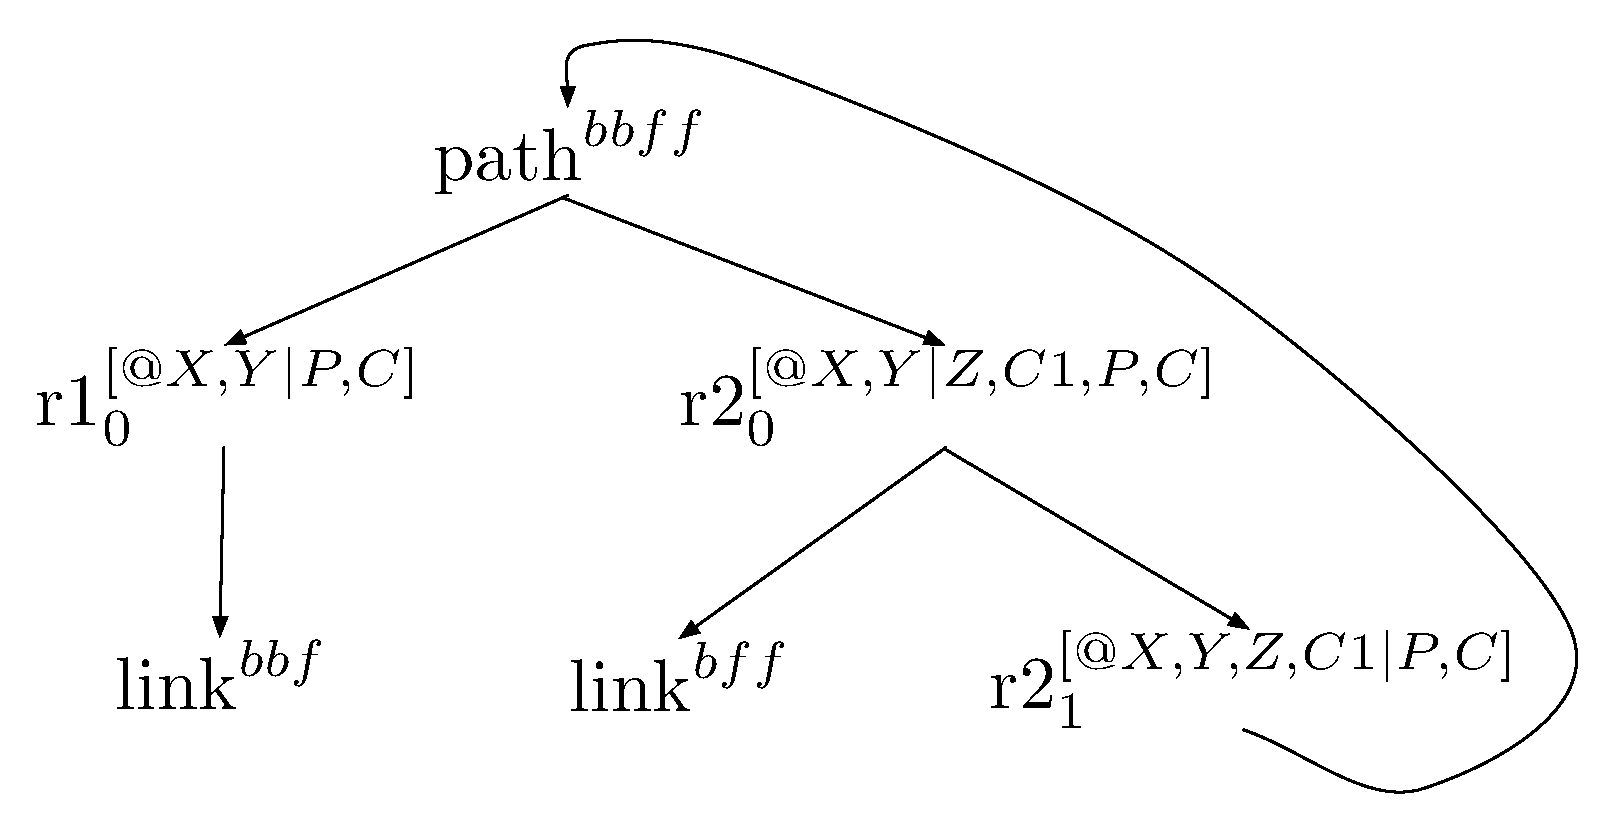
\includegraphics[scale=1.8]{figures/RuleGoalGraph}
\caption{Rule/Goal graph of the program in Figure~\ref{ch:evita:fig:querySP}.}
\label{ch:evita:fig:rggraph}
\end{center}
\end{figure*}

In the program analysis phase, the algorithm traverses every rule,
starting with those whose rule heads that match the query predicate, to build
a recursive tree structure called the {\em Rule/Goal} graph. This graph consists 
of \emph{rule} and \emph{goal} vertices.  A goal vertex consists of a predicate 
with an adornment indicating which of the attributes in the predicate are bound 
to a constant value and which are not (free).  A rule vertex represents the bound/free 
state of all seen variables within a rule body, up to a particular position in its left-to-right 
execution. A rule with $k$ body predicates will result in exactly $k$ rule vertices 
corresponding to its positions $[0,...,k-1]$.

Figure~\ref{ch:evita:fig:rggraph} illustrates the full {\em Rule/Goal} graph for our 
shortest path example.  To build this graph, the algorithm starts with a goal 
predicate (at first, this is the query predicate---\ol{path} in our example), and creates 
a goal vertex in the graph with the appropriate adornment ($\mathit{bbff}$ for
\ol{path} since the query binds its first two variables to constant values). For every
rule with that goal predicate as its head, the algorithm traverses the
rule body from left to right, creating a child rule vertex for every
$0$-th position variable binding.  For rule \ol{r2} in the example, the
rule vertex for position $0$ ($r_{2,0}$) has variable state $[X,Y|P,C]$,
which denotes that variables \ol{X,Y} are bound (to the same values as
those ``pushed down'' from the goal vertex) and \ol{P,C} are free.
Given a rule vertex for position $i$, two children are created: a goal
vertex for the next predicate after position $i$ and a rule vertex for
the next position in the rule (unless the body's end has been reached).
In the running example, the child goal vertex corresponds to the {\tt link} 
predicate that appears at position $0$, with adornment $\mathit{bff}$ 
since \ol{X} is already bound at this point in the evaluation, but \ol{Z, C1} are not.  
Similarly, the child rule vertex at position $1$ contains the variable signature 
$[X,Y,Z,C1|P,C]$ since \ol{link} added some bound variables.  The process 
continues until all rule and goal vertices have been constructed and connected; 
only a single goal vertex can exist with the same predicate and
adornment, as is the case for the \ol{path} vertex with adornment
$\mathit{bbff}$.  It is easy to see how the rest of the rule/goal graph is 
constructed. After all vertices have been generated given the chosen rules, 
any predicates with a unique adornment in the graph are added to the goals 
and the rules producing them are recursively traversed.


In the program rewrite phase, Ullman's algorithm traverses the rule/goal
graph generating magic predicates for each ``goal'' vertex that is
unique for its (IDB) predicate; in the example, there are multiple vertices
with different adornments for \ol{link}, but only one for \ol{path},
so only \ol{path} is chosen.  This magic predicate is inserted in
the $0$-th position of all rules with the corresponding goal predicate
as the rule head, with the bound variables of the signature as
attributes. In the example, the magic predicate for \ol{path} has the
form \ol{magic\_path(@X, Y)} since \ol{X, Y} are the bound 
variables in the signature of the ``goal'' vertex.  Also
\emph{supplementary} predicates are similarly created for all
encountered ``rule'' vertices during the graph traversal and inserted
within the corresponding original rule.  For example, {\tt sup\_r2\_1(@X,Y,Z,C1)} 
is created for ``rule'' vertex $r_{2,1}$ with the bound variables of
the adornments in the vertex, and placed in the original rule \ol{r2}
between the \ol{link} and \ol{path} predicates.


\begin{figure*}[!t]
\ssp
\begin{boxedminipage}{\linewidth}
{\bf link}("localhost:10000", "localhost:10001").\\
{\bf link}("localhost:10001", "localhost:10002").\\
...\\
{\bf magic\_path}(@LOCALHOST, "localhost:10000"). \\
\\
r1\_g3a {\bf path}(@X, Y, P, C) :- \\
\datalogspace {\bf magic\_path}(@X, Y), \\
\datalogspace {\bf link}(@X, Y, C), P := f\_cons(X, Y).\\
\\
r2\_g1a {\bf magic\_path}(@X, Y) :- \\
\datalogspace {\bf sup\_r2\_1}(@X, Y, Z, C1). \\
\\
r2\_g3a {\bf sup\_r2\_1}(@X, Y, Z, C1) :- \\
\datalogspace {\bf magic\_path}(@X, Y), \\
\datalogspace {\bf link}(@X, Z, C1). \\
\\
r2\_g3c {\bf path}(@X, Y, P, C) :- \\
\datalogspace {\bf sup\_r2\_1}(@X, Y, Z, C1), \\
\datalogspace {\bf path}(@Z, Y, P2, C2). \\
\datalogspace f\_contains(X, P2) == false, \\
\datalogspace P := f\_cons(X, P2), C := C1 + C2. \\
\\
Query: {\bf path}(@LOCALHOST, "localhost:10000", P, C).
\end{boxedminipage}
\caption{\label{ch:evita:fig:magicSP}A magic-sets rewrite of
      the rules in Figure~\ref{ch:evita:fig:querySP} (materialize statements not shown).}
\end{figure*}

Finally, in the filter population phase, the algorithm maintains the
magic predicate relation, which was placed within the rewritten program
in the previous phases.  Any a priori known bindings about the root goal vertex
(e.g., from the user's query) are placed in the magic relation. In the example, the 
fact ``\ol{magic\_path(LOCALHOST, "localhost:10000").}'' is put into the
database from the bindings in the \ol{path} query.  Also, any edges in
the rule/goal graph that start from a rule vertex and end at a goal vertex, with a
unique adornment (i.e., upward arrows in the recursive tree that constitutes the graph), are written as
rules that generate new magic tuples from new tuples of the rule
node's supplementary predicate. In the example, rule \ol{r2\_g1a}~\footnote{Rule names that
deal with magic and supplementary predicate maintenance were named according
to Ullman's rule groups. For instance, rules named \ol{r*\_g3[a-c]} follow rule group 3
and rule \ol{r2\_g1a} follows rule group 1.}  adds
more magic facts as more \ol{sup\_r2\_1} tuples are produced.

Our rewrite implementation of this algorithm first traverses every rule
from head predicate to body predicates from left to right, constructing
the rule/goal graph in the recursive manner of the program analysis, in
a single fixpoint.  Then the new program rules (and replacement of old
rules) for the program rewrite and filter population phases are
performed via a traversal of the newly constructed rule/goal graph in a
subsequent fixpoint. Finally, initial magic facts are created by direct
translation from the query.  Other details that we elide here involve detecting 
eligibility of a predicate for a magic-sets rewrite (whether or not it has a unique 
adornment in the rule/goal graph), state cleanup, etc. 

\begin{figure*}
\ssp
\begin{boxedminipage}{\linewidth}
{\bf materialize}(sup,infinity,infinity,keys(2,3,4)). \\
{\bf materialize}(adornment,infinity,infinity,keys(2,5,6)). \\
{\bf materialize}(idbPredicate,infinity,infinity,keys(2,3)). \\
\\
mg1 {\bf goalCount}(@A, Pid, PredName, a\_count$<*>$) :- \\
\datalogspace {\bf idbPredicate}(@A, Pid, PredName), \\
\datalogspace {\bf adornment}(@A, Pid, Rid, Pos, PredName, Sig). \\
\\
mg2 {\bf magicPred}(@A, Pid, GoalName, Sig) :- \\
\datalogspace {\bf goalCount}(@A, Pid, GoalName, Count), \\
\datalogspace {\bf adornment}(@A, Pid, \_, \_, GoalName, Sig). \\
\datalogspace Count == 1. \\
\\
mg3 {\bf sup}(@A, Pid, Rid, Pos, Name, Schema) :- \\
\datalogspace {\bf magicPred}(@A, Pid, Name, Sig), \\
\datalogspace {\bf rule}(@A, Rid, Pid, \_, HeadPid, \_, \_, \_), \\
\datalogspace {\bf predicate}(@A, HeadPid, Rid, \_, Name, \_, \_, Schema, \_, \_, \_), \\
\datalogspace Schema := {\em f\_project}(Sig, Schema), \\
\datalogspace Name := "magic\_" + Name, Pos := 0. \\
\\
mg4 {\bf supNext}(@A, Pid, Rid, Pos+1, Schema) :- \\
\datalogspace {\bf sup}(@A, Pid, Rid, Pos, Name, Schema). \\
\\
mg5 {\bf sup}(@A, Pid, Rid, Pos, Name, Schema) :- \\
\datalogspace {\bf supNext}(@A, Pid, Rid, Pos, PrevSupSchema),\\
\datalogspace {\bf rule}(@A, Rid, Pid, RuleName, \_, \_, \_, \_),\\
\datalogspace {\bf predicate}(@A, \_, Rid, \_, \_, \_, \_, Schema, Pos, \_, \_),\\
\datalogspace Name := "sup\_" + RuleName + "\_" + {\em f\_tostr}(Pos),\\
\datalogspace Schema := {\em f\_merge}(PrevSupSchema, PredSchema).\\
\\
mg6 {\bf adornment}(@A, Pid, Rid, Pos, PredName, Sig) :- \\
\datalogspace {\bf supNext}(@A, Pid, Rid, Pos, PrevSupSchema),\\
\datalogspace {\bf idbPredicate}(@A, Pid, PredName), \\
\datalogspace {\bf rule}(@A, Rid, Pid, \_, \_, \_, \_, \_),\\
\datalogspace {\bf predicate}(@A, \_, Rid, \_, PredName, \_, \_,Schema, Pos, \_, \_),\\ 
\datalogspace Sig := {\em f\_adornment}(PrevSupSchema, Schema).
\end{boxedminipage}
\caption{\label{ch:evita:fig:magicRules}Rule/Goal graph traversal rules.}
\end{figure*}

To give a flavor of the \OVERLOG implementation of magic-sets,
Figure~\ref{ch:evita:fig:magicRules} shows six rules that build the state
necessary in the magic-sets rewrite by traversing the rule/goal graph. 
The \ol{adornment} predicate contains the predicate name ($PredName$) and an
adornment string ($Sig$), which is initially populated (by a single rule, not shown) with
the query predicate adornments. Rule \ol{mg1} counts the number of
adornments for each {\em IDB} predicate. If this count is unique ($Count == 1$) in rule \ol{mg2},
then a \ol{magicPred} tuple is created. Rule \ol{mg3} triggers on a \ol{magicPred} tuple and, for each
rule whose head predicate is named by the \ol{magicPred} tuple, it generates a \ol{sup} predicate
with a $Schema$ attribute containing the bound variables that exist at the given rule position. 
Rule \ol{mg4} detects a new \ol{sup} predicate (like the one generated for the rule head) and triggers 
an event for the subsequent \ol{sup} predicate position in the given rule. The three way join in rule \ol{mg5} 
produces a tuple that contains the schema of the previous \ol{sup} predicate ($PrevSupSchema$) 
and the schema of the predicate ($Schema$) in the subsequent rule position, should one 
exist~\footnote{Two rules (not shown) move the \ol{supNext} position forward if the given rule position does 
not identify a predicate.}. The head \ol{sup} predicate schema in rule \ol{mg5} contains all the variables from the 
previous \ol{sup} predicate and the schema of the current predicate, since this schema represents the bound variables
that will exist in the subsequent rule position. Rule \ol{mg6} creates an \ol{adornment} out of the predicate 
in the given rule position, if that predicate is part of the {\em IDB}. The {\em f\_adornment} 
function creates a new signature from the bound variables in the $PrevSupSchema$ attribute, 
and the variables in the predicate $Schema$ attribute. At the end of the rule/goal graph traversal, 
those predicates that define a unique adornment become magic predicates, and the rules that mention 
these magic predicates are rewritten using the information contained in the \ol{sup} table.

\subsubsection{Magic-sets in the Network}

With the details of the magic-sets algorithm behind us, what is
intuitively happening to the shortest-path snippet in
Figure~\ref{ch:evita:fig:magicSP} is that variable bindings in the query are
recursively translated into filtering magic and supplementary
predicates. Since the query is only looking for paths to
destination ``localhost:10000'', at first the magic fact restricts single-hop
paths created from links in rule \ol{r1}) to only those with that same 
destination (in the rewritten rule \ol{r1\_g3a}). Similarly, in what used to 
be rule \ol{r2}, {\tt link} tuples are filtered according to the magic predicate (in rule
\ol{r2\_g3a}), before being joined with existing \ol{path} tuples to
complete the old rule \ol{r2}. The reason rule \ol{r2} was split into
the two rules \ol{r2\_g3a} and \ol{r2\_g3c} is because the
supplementary result \ol{sup\_r2\_1} is useful towards adding extra bindings as
magic tuples (in rule \ol{r2\_g1a}); this is because any variable
binding that survives filtering right before the \ol{path}
predicate in the body of the old rule \ol{r2} is also an interesting
binding for existing or future \ol{path} tuples. If the original
program had not been recursive, then such recursive definitions of magic
facts would not appear in the rewritten program.

\begin{figure*}
\centering

\includegraphics[scale=1.2]{figures/Topology}
\caption{Experimental topology.}
\label{ch:evita:fig:topo}
\end{figure*}

To understand the effects of this rewrite, we describe two experimental
runs of our program, before and after the magic-sets rewrite (both
programs were also subjected to the localization rewrite from
Section~\ref{ch:evita:sec:localization} since they are distributed).  The two
programs are executed in the simple link topology of
Figure~\ref{ch:evita:fig:topo}. Nodes are started up one at a time in order of
identifier, and the preloaded database (EDB) consists of the links pictured. For each experiment we measure the number of
tuples sent and received by each node, as well as any \ol{path}
tuples constructed. The latter measure is meant to convey ``work''
performed by the distributed program even in local computation that does
not appear on the network (e.g., local tuple computations, storage, and
other dependent actions on those tuples).

\begin{figure*}
\centering
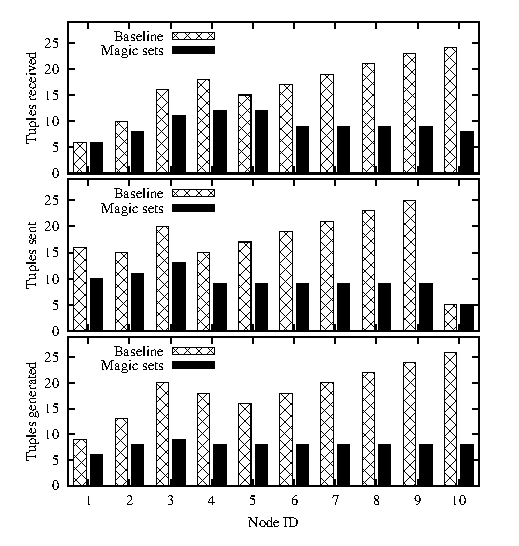
\includegraphics{figures/magicNumbers}
\ssp
\caption{For each node (node ID on $x$ axis), number of tuples received
  (top), sent (middle), and locally generated (bottom) on the $y$ axis.}
\label{ch:evita:fig:magicresults}
\end{figure*}

Figure~\ref{ch:evita:fig:magicresults}(a) shows the number of tuples that each node receives from
the network. The magic-sets rewritten program causes no more tuples to
be received than the original, and for most nodes significantly fewer
when moving to nodes farther away from the clique. That is because many
paths that are generated in the original program with destinations
within the clique other than node $1$ are pruned early on and never
transmitted all the way to the far end.    Similarly,
Figure~\ref{ch:evita:fig:magicresults}(b) shows the number of tuples each node transmits.
Again, the magic-rewritten program does a lot better.  The two programs
have similar tuple transmit/receive overheads for nodes represents the number of tuples a node sends out
over the network. The inclusion of the magic-sets rewrite reduces the number of sends
in all but one case (node $10$). The node with identifier $10$ is the only node with 
no incoming links and 
is therefore never burdened with network traffic other than its
own; as a result, though its received tuple overhead benefits from magic
sets, it transmitted tuple overhead is unaffected, since it already
sends out no extraneous paths other than its sole path towards node $1$.
Finally, tuple storage is impacted beneficially by magic sets everywhere
(Figure~\ref{ch:evita:fig:magicresults}(c)), since
both \ol{path} tuples received from the network, but also those
generated locally for local consumption are pruned away by the rewrite.



\subsection{Localization}
\label{ch:evita:sec:localization}

Finally, we briefly describe the localization compiler stage, which turns
a rule with  multiple
location specifiers in its body to many rules, each of which has a
single location specifier in its body; this essentially turns a
distributed join into a set of local joins with partial result
transmissions among the rules involved~\cite{loo-sigmod06}. This rewrite
is part of the P2
system, but implemented in C++ and woven into the monolithic compiler.

In Evita Raced, localization stage traverses distributed rules in
left-to-right order starting with first body predicates (rules with
local-only body predicates are selected out early in the stage). 
The location attribute of the current predicate in this traversal is noted at each iteration.
A {\em breakpoint} is generated if the traversal reaches a predicate with location attribute 
that differs from the previous. The breakpoint triggers a {\em split} rule at the given 
position, which creates a new {\em glue} predicate $IR_p$, and two new rules defined as follows.
\begin{CompactEnumerate}
\item $IR_p$ :- (predicates to the left, excluding the breakpoint).
\item (original rule head predicate) :- $IR_p$, (predicates to the right, including the breakpoint). 
\end{CompactEnumerate}
The location attribute in the $IR_p$ predicate is taken from the predicate at the breakpoint position.
The other attributes in the $IR_p$ predicate are taken from the predicates to the left of (and not 
including) the breakpoint, which represents the schema of the intermediate result prior to the
breakpoint position predicate. The algorithm then removes the original rule, and moves recursively on
the second rule, which is considered the original rule in the above discussion. 
The recursion terminates at the rightmost predicate position. 

The localization stage is not an optimization per se, but rather a  program rewrite necessary to make distributed rules executable. 
% Any program that contains distributed rules must go through this compilation stage. 
The \OVERLOG program for localization consists of only 28 rules. The original P2
code that performed this task in P2 consisted of approximately 400 lines of
% carefully crafted 
C++.  


\section{Discussion}
\label{ch:evita:sec:discussion}

When we started this work, the vision of declaratively specified query optimization was appealing 
thanks to its elegance and its promise of usability and maintainability.  Although we remain convinced 
on this front, our optimism has been tempered by the pragmatics of developing software within a
continuously changing system prototype. Here we reflect on some of the (hard) lessons we learned 
while conducting this research.

P2's notion of consecutive Datalog-style fixpoints, especially in networked environments, still has 
many rough edges, both on the design and on the engineering front.  Because deep down P2's runtime 
is an event-driven execution engine, its basic unit of atomicity is akin to a single iteration 
through a recursive query evaluation strategy like semi-naive evaluation, generating a set of 
derived actions (tuples to be inserted, deleted, transmitted remotely, or evaluated locally for 
further deduction) from a single incoming event, and committing changes to the database atomically 
upon completion of such a step~\cite{LuThesis}. P2's Datalog-style fixpoints are implemented as 
sequences of such single-event iterations, in a manner that appears to have been an afterthought. 
As a result, the system's design shares both event-driven and logic-style flavors, with some 
remaining unresolved conflicts, and no explicit language constructs to bridge between the two.

One example is the notion of \ol{delete} rules, the semantics of which are unclear.  How is one to 
handle delete rules triggered by the \emph{deletion} of a base tuple?  The system certainly does 
not support -- semantically or operationally -- the ``undeleting'' of tuples that were
originally deleted due to a base fact that is no longer in the database.  Similarly, the semantics 
for multiple updates to the same tuple within the same fixpoint are undefined and a local tie
breaking rule is chosen to decide on a consistent ordering among same-fixpoint updates to the 
same relation. Compiler stages that do static analysis might catch such dangerous rules and alert the user.

Second, as in most prototypes, the programmer interface is not polished. Debugging is difficult, especially 
since the logic language makes it tough to understand which value corresponds to which formal
attribute in a long tuple of a dozen or more attributes.  Though concise, declaratively specified 
optimizations pack a punch in terms of density of concepts, which only becomes deadlier due to the (otherwise
desirable) arbitrary order of rule execution.  Certainly a better thought-out system to debug declarative 
programs -- optimizations, no less -- would have made the job easier.  To be fair, however, our
experience with building monolithic optimizers in production database management systems in the past 
was not a great deal rosier.  It is hard to debug code when the output's correctness (e.g., minimality of cost) 
is too expensive to verify.

Third, the evolution of the \OVERLOG language has a long way to go. The language still offers no modularity, 
making it tough to isolate and reuse logically distinct components. It does has a rudimentary concrete
type system, but has poor support for structured types like matrices and lists.  \OVERLOG still ``cuts corners'' 
on the proper set-orientation of Datalog; since program stratification is only preliminary in
the system prototype, dealing with streaming aggregates in the face of EDB updates required us to 
resort to imperative tricks like timers and polling to determine that aggregates were ready to be finalized.

Beyond particular characteristics of P2, one hard lesson we learned was that extensibility and ease of use at 
the top often comes at the expense of complexity below the extensibility layer.  The tabularization of
compiler state to enable declarative optimizations also meant that even imperative compiler stages such as our
bootstrap stages implemented in C++ had to use tables, foregoing their familiar interaction with C++ data 
structures.  Building glue libraries that ease this interaction may relieve this pain.

Nevertheless, despite these complaints, we were able to get all of our desired optimizations expressed 
in \OVERLOG in a highly compact way, as promised by the various earlier papers on P2.  By contrast, the 
initial version of P2 had no query optimizations of interest beyond localization.  As \OVERLOG and P2 mature, 
the use of a metacompilation approach should get even easier.  And based on our initial experience 
extending \OVERLOG with security properties in a manner similar to~\cite{abadi-netdb07}, we believe that 
our Evita Raced infrastructure could accelerate the ability of the P2 group to pursue modifications to 
\OVERLOG itself.

\section{Summary}
\label{ch:evita:sec:summary}
The Evita Raced metacompilation framework allows \OVERLOG compilation tasks to be written in \OVERLOG and
executed in the P2 runtime engine. It provides significant extensibility via a relatively clean declarative
language. Many of the tasks of query optimization -- dynamic programming, dependency-graph construction
and analysis, statistics gathering -- appear to be well served by a recursive query language. The notion of
metacompilation also leads to a very tight implementation with significant reuse of code needed for
runtime processing.

Even with the caveats expressed in Section~\ref{ch:evita:sec:discussion}, we are convinced that a declarative metacompiler
is much easier to program and extend than the monolithic query optimizers we have worked on previously.
We are now at a  point where we can add significant features (e.g., histograms, broadcast rewrites, 
stratification tests) in an hour or two, where they would otherwise have taken days or weeks of work
in a traditional implementation. 

One surprising lesson of our work was the breadth of utility afforded by the metacompilation framework. Although
motivated by performance optimizations, we have used Evita Raced for a number of unforeseen tasks. These
include: automatically expanding user programs with instrumentation and monitoring logic; generating pretty-printers
for intermediate program forms; language wrappers for secure networking functionality in the manner of
SecLog~\cite{abadi-netdb07}; stratification detectors and other static code analysis. None of these are performance optimizations
per se, but all fit well within an extensible, declarative program manipulation framework. More generally, we believe
that metacompilation is a good design philosophy not only for our work, but for the upcoming generation of
declarative engines being proposed in many fields. 


\chapter[MapReduce: An Elephant's Perspective]{MapReduce: An Elephant's Perspective}
\label{ch:hadoop}

In this chapter, we review the MapReduce programming
model~\cite{mapreduce-osdi} and the Hadoop system~\cite{hadoop} --- an
open-source software framework that supports data-intensive distributed
applications.  We focus on those aspects of the Hadoop system kernel that
concern the remaining chapters of this thesis.  We begin in
Chapter~\ref{ch:hadoop:sec:progmodel} with the MapReduce programming model,
which is based on two operations: {\em map} and {\em reduce}.
Chapter~\ref{ch:hadoop:sec:hadoop} discusses the Hadoop implementation, which
is comprised of a MapReduce dataflow engine, inspired by Google's
MapReduce~\cite{mapreduce-osdi}, and a distributed file system that models the
Google File System (GFS)~\cite{gfs-sosp}.  Chapter~\ref{ch:hadoop:sec:conclude}
contains a high-level description our work in this area; postponing the details
to remaining chapters of this thesis.

\section{MapReduce Programming Model}
\label{ch:hadoop:sec:progmodel}

MapReduce programmers expresses their computations as a series of {\em jobs}
that process collections of data in the form of key-value pairs . Each job
consists of two stages: first, a user-defined \ol{map} function is applied to
each input record to produce a list of intermediate key-value pairs.  Second, a
user-defined \ol{reduce} function is called on each distinct key and
list of associated values from the map output, and returns a list of output
values.  The MapReduce framework automatically parallelizes the execution of
these functions and ensures fault tolerance.

Optionally, the user can supply a \ol{combiner}
function~\cite{mapreduce-osdi}, which will be applied to the intermediate
results between the map and reduce steps.  Combiners are similar to reduce
functions, except that they are not passed {\em all} the values for a given
key: instead, a combiner emits an output value that summarizes the input values
it was passed.  Combiners are typically used to perform map-side
``pre-aggregation,'' which reduces the amount of network traffic required
between the map and reduce steps.

\section{Hadoop MapReduce}
\label{ch:hadoop:sec:hadoop}

Hadoop is composed of {\em Hadoop MapReduce}, an implementation of MapReduce
designed for large clusters, and the {\em Hadoop Distributed File System}
(HDFS), a file system optimized for batch-oriented workloads such as MapReduce.
In most Hadoop jobs, HDFS is used to store both the input to the map step and
the output of the reduce step.  Note that HDFS is {\em not} used to store
intermediate results (e.g., the output of the map step): these are kept on each
node's local file system.

A Hadoop installation consists of a single master node and many worker nodes.
The master, called the {\em JobTracker}, is responsible for accepting jobs
from clients, dividing those jobs into {\em tasks}, and assigning those tasks
to be executed by worker nodes.  Each worker runs a {\em TaskTracker} process
that manages the execution of the tasks currently assigned to that node.  Each
{\TT} has a fixed number of slots for executing tasks (two maps and two reduces
by default).  A heartbeat protocol between each {\TT} and the {\JT} is used to
update the {\JT}'s bookkeeping of the state of running tasks, and drive the
scheduling of new tasks: if the \JT identifies free {\TT} slots, it will
schedule further tasks on the {\TT}.

\subsection{Map Task Execution}
\label{ch:hadoop:sec:maptask}

\begin{figure*}[t]
\ssp
\begin{minipage}{\linewidth}
\centering
\begin{verbatim}
public interface Mapper<K1, V1, K2, V2> {
  
  void map(K1 key, V1 value, OutputCollector<K2, V2> output);

  void close();
}
\end{verbatim}
\end{minipage}
\caption{Map function interface (Hadoop version 18.2).}
\label{fig:mapfunction}
\end{figure*}

Each map task is assigned a portion of the input file called a {\em split}.
By default, a split contains a single HDFS block (64MB by default), so the
total number of file blocks determines the number of map tasks.

The execution of a map task is divided into two phases.
\begin{enumerate}
    \ssp
\item
  The {\em map} phase reads the task's split from HDFS, parses it into
  records (key/value pairs), and applies the map function to each
  record.
\item
  After the map function has been applied to each input record, a
  {\em commit} phase registers the final output with the {\TT}, which
  then informs the {\JT} that the task has finished executing.
\end{enumerate}

Figure~\ref{fig:mapfunction} contains the interface that must be implemented by
user-defined map functions.  After the \ol{map}
function has been applied to each record in the split, the \ol{close} method is
invoked.  The third argument to the \ol{map} method specifies an {\em
OutputCollector} instance, which accumulates the output records produced by the
map function.  The output of the map step is consumed by the reduce step, so
the {\em OutputCollector} stores map output in a format that is easy for reduce
tasks to consume.  Intermediate keys are assigned to reducers by applying a
partitioning function, so the {\em OutputCollector} applies that function to each key
produced by the map function, and stores each record and partition number in an
in-memory buffer.  The {\em OutputCollector} spills this buffer to disk when it
reaches capacity.

A spill of the in-memory buffer involves first sorting the records in the
buffer by partition number and then by key.  The buffer content is written to
the local file system as an index file and a data file
(Figure~\ref{ch:hadoop:fig:mapoutput}).  The index file points to the offset of
each partition in the data file.  The data file contains only the records,
which are sorted by the key within each partition segment.

During the {\em commit} phase, the final output of the map task is generated
by merging all the spill files produced by this task into a single pair of data
and index files.  These files are registered with the {\TT} before the task
completes.  The \TT will read these files when servicing requests from reduce
tasks.

\begin{figure}[t]
  \ssp
  \centering
  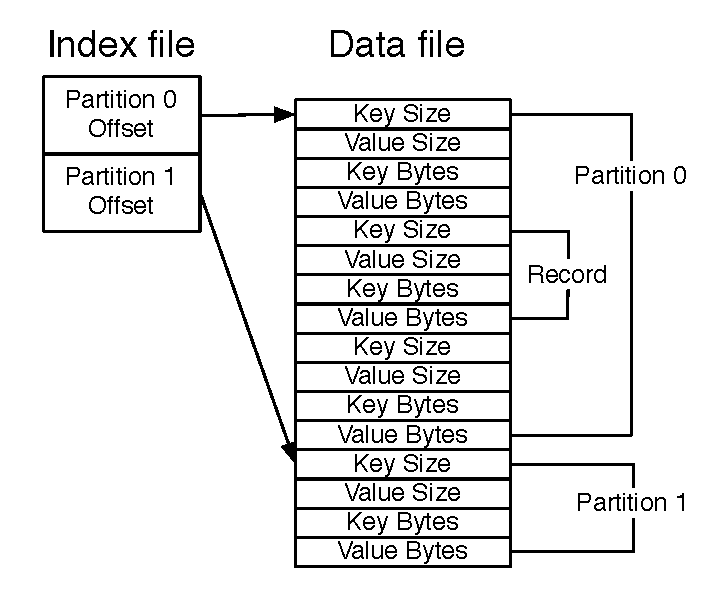
\includegraphics[scale=0.8]{figures/spill_file.pdf}
  \caption{Map task index and data file format (2 partition/reduce case).}
  \label{ch:hadoop:fig:mapoutput}
\end{figure}

\subsection{Reduce Task Execution}
\label{ch:hadoop:sec:reducetask}
The execution of a reduce task is divided into three phases.
\begin{enumerate}
    \ssp
\item The {\em shuffle} phase fetches the reduce task's input
  data. Each reduce task is assigned a partition of the key range
  produced by the map step, so the reduce task must fetch the content
  of this partition from every map task's output.
\item The {\em sort} phase groups records with the same key together.
\item The {\em reduce} phase applies the user-defined reduce function
  to each key and corresponding list of values.
\end{enumerate}

In the {\em shuffle} phase, a reduce task fetches data from each map task by
issuing HTTP requests to a configurable number of {\TT}s at once (5 by
default).  The {\JT} relays the location of every {\TT} that hosts map output
to every {\TT} that is executing a reduce task.  Note that a reduce task cannot
fetch the output of a map task until the map has committed its final output to
disk.

\begin{figure*}[t]
\ssp
\begin{minipage}{\linewidth}
\begin{verbatim}
public interface Reducer<K2, V2, K3, V3> {

  void reduce(K2 key, Iterator<V2> values, OutputCollector<K3, V3> output);

  void close();
}
\end{verbatim}

\end{minipage}
\caption{Reduce function interface (Hadoop version 18.2).}
\label{fig:reducefunction}
\end{figure*}

After receiving its partition from all map outputs, the reduce task enters the
{\em sort} phase~\footnote{Some pre-sorting work is done during the shuffle
phase.}.  The map output for each partition is already sorted by the reduce
key.  Therefore, the reduce task will merge these runs together to produce a
single run that is sorted by key.  The task then enters the {\em reduce} phase,
during which it invokes the user-defined reduce function for each distinct key
(in sorted order) and associated list of values.  The output of the reduce
function is written to a temporary location on HDFS.  After the reduce function
has been applied to each key in the reduce task's partition, the task's HDFS
output file is atomically renamed from its temporary location to its final
location.

In this design, the output of both map and reduce tasks is written to disk
before it can be consumed. This is particularly expensive for reduce tasks,
because their output is written to HDFS\@. Output materialization simplifies
fault tolerance, because it reduces the amount of state that must be restored to
consistency after a node failure. If any task (either map or reduce) fails, the
{\JT} simply schedules a new task to perform the same work as the failed
task. Since a task never exports any data other than its final answer, no
further recovery steps are needed.

 % Mention fault-tolerance/atomic
% rename here?

% \subsection{Dataflow in Hadoop}
% Hadoop \emph{materializes} the output of the map and reduce functions
% in two places:

% \begin{itemize}
% \item
%   Between the map and reduce steps, the output of each map task is
%   written to disk before it can be read by any reduce tasks.
% \item
%   The output of the reduce step is written to HDFS at the end of each
%   job. As we observed in Section~\ref{sec:progmodel}, many practical
%   computations are written as a chain of MapReduce computations
%   (e.g.\ PageRank). In that setting, writing the output of each job to
%   HDFS and then reading it back again is inefficient.
% \end{itemize}



\section{Summary}
\label{ch:hadoop:sec:conclude}

The MapReduce interface is a good example of capturing the minimum essentials
of an abstraction, making it easy to build many higher-order constructs (e.g.,
data analysis~\cite{pig-sigmod}, SQL~\cite{hive-vldb}, machine
learning~\cite{mahout}) while allowing significant flexibility in the system
implementation.  Fault-tolerance was an early part of the MapReduce system
design, and one of its most attractive features.  The fault-tolerance model is
predicated on the batch-oriented nature of MapReduce, allowing the recovery of
a task to simply be restarting it on some (possibly alternate) machine.  Since
no state, in the form of output data, is allowed to exit a task (map or
reduce), no further recovery actions are required.

Optimization at the MapReduce level often comes in the form of scheduling
policies that primarily focus on job response time.  The runtime of a MapReduce
job is determined by its slowest tasks.  The slowest map task determines the
finishing time of the {\em shuffle} phase since reduce tasks are not able to
enter the {\em reduce} phase until they have received all the map outputs that
belong to them.  The slowest reduce task determines the finishing time of the
overall job since a job does not complete until all reduce tasks complete.
Speculation is a response-time optimization that executes clones of tasks
deemed to be slow.  Alternative speculation policies for identifying and
speculatively scheduling these 'straggler' tasks exist~\cite{mapreduce-osdi,
zaharia-late}, but there is no consensus on a policy that works well for all
jobs and cluster configurations.

In Chapter~\ref{ch:boom}, we describe an implementation of the Hadoop MapReduce
engine in the \OVERLOG language.  This declarative specification of Hadoop
enables us to build alternative scheduling policies and optimizations in a high
level query language improving the development cycle and decreasing the lines
of code by {\em orders of magnitude}, all while supporting a richer suite of
scheduling strategies.  In Chapter~\ref{ch:hop}, we move from a batch-oriented
execution model to a pipelined model where tasks incrementally send their
output.  Pipelining enables two new features in the context of MapReduce:
online aggregation~\cite{onlineagg} and continuous queries.  We show that a
pipelined implementation of MapReduce does not sacrifice the original system
interface or its ability to tolerate faults.  A pipelined MapReduce model
extends the range of scheduling alternatives, which we easily support through
policies written in \OVERLOG.


\chapter[Declarative Scheduling]{Declarative Scheduling}
\label{ch:boom}

The Berkeley Orders Of Magnitude (BOOM) project began with an experiment in
construction, by implementing a substantial piece of distributed software in a
data-centric, declarative style.  Upon review of recent literature on
data center infrastructure (e.g.,~\cite{chubby,gfs-sosp,dynamo,mapreduce-osdi}),
we observed that most of the complexity in these systems relates to the
management of various forms of asynchronously-updated state, including
sessions, protocols and storage.  Although quite complex, few of these systems
involve intricate, uninterrupted sequences of computational steps.  Hence, we
suspected that data center infrastructure might be a good initial litmus test
for our hypotheses about building distributed software.

We evaluated this hypotheses in {\em \BOOMA}: an API-compliant reimplementation
of the HDFS distributed file system and the Hadoop MapReduce
engine~\cite{boom}.  Our declarative version of these two components were named
{\em \BOOM-FS} and {\em \BOOM-MR}, respectively.  In writing \BOOMA, we
preserved the Java API ``skin'' of HDFS and Hadoop, but replaced complex
internal state with a set of relations, and implemented key system logic with
code written in a declarative language.  In this thesis, we focus on
declarative scheduling (\BOOM-MR), but include some experimental results that
show \BOOM-FS performance is on par with HDFS.

The remainder of this chapter is organized as follows.
Chapter~\ref{ch:boom:sec:jol} describes a new Java-based \OVERLOG library,
which we used execute \OVERLOG programs within the (Java-based) Hadoop
infrastructure.  In Chapter~\ref{ch:boom:sec:port}, we discuss the \BOOM-MR
scheduling harness; embedded in the \JT component of Hadoop.
Chapter~\ref{ch:boom:sec:hadoop} reviews the scheduling state and
protocol---implemented in Hadoop version 18.2---that we modeled in our
declarative code.  Chapter~\ref{ch:boom:sec:tables} captures the entities
and relationships of the Hadoop scheduler in four (catalog) tables.  Using these
tables, we develop a scheduling policy in Chapter~\ref{ch:boom:sec:scheduler}
that models the Hadoop FIFO policy.  We then extend these rules in
Chapter~\ref{ch:boom:sec:late} with the LATE policy for scheduling ``speculative''
tasks.  Our declarative LATE port took {\em orders of magnitude} less time and
code than the (logically) equivalent Java port~\cite{jira-2141}; once the basic
relational infrastructure was in place.  Chapter~\ref{ch:boom:sec:eval}
evaluates the performance of jobs scheduled by our declarative FIFO policy
against those scheduled by the original (unmodified) Hadoop scheduler.
Finally, Chapter~\ref{ch:boom:sec:relwork} examines some of the related work
and Chapter~\ref{ch:boom:sec:conclusion} concludes with a summary of our
experience with \BOOMA.

\section{Java \OVERLOG Library (JOL)}
\label{ch:boom:sec:jol}

In previous chapters we saw that P2's lack of support for stratified Datalog
forced us to implement a number of imperative hacks, which often involved
(event) manipulations of the underlying dataflow fixpoints.  Most of these
hacks were required for detecting the termination of a group of rules, which
would have been implicitly handled by imposing a natural stratum boundary
(e.g., count aggregate).  Our workaround involved adding a number of conditions
that detected stratum boundaries, and ensured that these ``conditions'' were
evaluated in separate P2 dataflow fixpoints.  This was a hard lesson, which led
us to develop an entirely new \OVERLOG implementation that supports stratified
Datalog.  We briefly describe this new Java \OVERLOG Library (JOL), which we
used to implement the remaining \OVERLOG programs described in this thesis.

Like P2, \JOL compiles \OVERLOG programs into pipelined dataflow graphs of
operators (similar to ``elements'' in the Click modular router~\cite{click}).
\JOL provides {\em metaprogramming} support akin to P2's Evita Raced
extension (Chapter~\ref{ch:evita}): each \OVERLOG program is compiled into a
representation that is captured in rows of tables.  Program testing,
optimization and rewriting can be written concisely as metaprograms in \OVERLOG
that manipulate those tables.

The \JOL system matured when we targeted the Hadoop stack, which required tight
integration between \OVERLOG and Java code.  The latest version of \JOL
includes Java-based extensibility in the model of Postgres~\cite{postgres}.  It
supports Java classes as abstract data types, allowing Java objects to be
stored in fields of tuples, and Java methods to be invoked on those fields from
\OVERLOG.  \JOL also allows Java-based aggregation functions to run on sets of
column values, and supports Java {\em table functions}: Java iterators
producing tuples, which can be referenced in \OVERLOG rules as ordinary
relations.  We made significant use of each of these features in \BOOMA.

%In addition, inspired by the ideas of Evita Raced, we metaprogrammed \JOL's
%core execution loop and scheduler in \OVERLOG as well.  Rather than using a
%traditional event loop, in \JOL all inbound events (i.e., tuples) are passed
%into a single dataflow compiled from the system's runtime metaprogram.  This
%dataflow ``routes'' tuples to appropriate branches corresponding to different
%rules, using a scheduler specified in \OVERLOG.  Space prevents a thorough
%discussion of this design, but we mention it here because of our experience
%modifying the runtime rules as described in Chapter~\ref{sec:perf}.

\section{\BOOM-MR: MapReduce Scheduler}
\label{ch:boom:sec:port}

In this section, we describe our declarative version of the Hadoop MapReduce
scheduled, which we call \BOOM-MR.  Using \BOOM-MR, we explored embedding a
data-centric rewrite of a non-trivial component into an existing procedural
system.  MapReduce scheduling policies are one issue that has been treated in
recent literature (e.g.,~\cite{zaharia-late,delay-sched}).  To enable credible
work on MapReduce scheduling, we wanted to remain true to the basic structure
of the Hadoop MapReduce codebase, so we proceeded by understanding that code,
mapping its core state into a relational representation, and then writing
\OVERLOG rules to manage that state in the face of new messages delivered by
the existing Java APIs. 

\subsection{Hadoop MapReduce Scheduler}
\label{ch:boom:sec:hadoop}

We briefly review the Hadoop scheduling logic that we modeled in \OVERLOG.  The
Hadoop architecture consists of a single master node called the {\em \JT} that
manages a number of worker nodes called {\em {\TT}s}.  A job is divided into a
set of map and reduce {\em tasks}.  The {\JT} assigns tasks to worker nodes.
Each map task reads an input chunk from the distributed file system, runs a
user-defined map function, and partitions output key/value pairs into hash
buckets on the local disk.  Reduce tasks are created for each hash bucket.
Each reduce task fetches the corresponding hash buckets from all mappers, sorts
locally by key, runs a user-defined reduce function and writes the results to
the distributed file system.

Each {\TT} has a fixed number of slots for executing tasks (two maps and two
reduces by default).  A heartbeat protocol between each {\TT} and the {\JT} is
used to update the {\JT}'s bookkeeping of the state of running tasks, and drive
the scheduling of new tasks: if the {\JT} identifies free {\TT} slots, it will
schedule further tasks on the {\TT}.  Also, Hadoop will attempt to schedule
{\em speculative} tasks to reduce a job's response time if it detects
``straggler'' nodes~\cite{mapreduce-osdi}.

\subsection{Table-izing MapReduce}
\label{ch:boom:sec:tables}

\BOOM-MR is a port of the Hadoop \JT code to \OVERLOG.  In this chapter, we
identify the key state maintained by the {\JT}.  This state includes both data
structures to track the ongoing status of the system and transient state in the
form of messages sent and received by the {\JT}.  We captured this information
the four \OVERLOG tables shown in Table~\ref{ch:boom:tbl:hcatalog}.

\begin{table}
\ssp
\centering
\begin{tabular}{|l|l|l|} \hline
\textit{Name}   & \textit{Description} & \textit{Relevant attributes} \\ \hline\hline
job         & Job definitions   & \underline{JobId}, Priority, SubmitTime, Status, JobConf \\ \hline
task         & Task definitions  & \underline{JobId}, \underline{TaskId}, Type, Partition, Status \\ \hline
taskAttempt  & Task attempts      & \underline{JobId}, \underline{TaskId}, \underline{AttemptId}, Progress, \\
             &       & State, Phase, Tracker, InputLoc, Start, Finish \\ \hline
taskTracker  & {\TT} State  & \underline{Name}, Hostname, State, \\
             &       & MapCount, ReduceCount, MaxMap, MaxReduce\\ \hline
\end{tabular}
\caption{\BOOM-MR relations defining {\JT} state.}
\label{ch:boom:tbl:hcatalog}
\end{table}

The \ol{job} relation contains a single row for each job submitted to the
{\JT}.  In addition to some basic metadata, each job tuple contains an
attribute called the $JobConf$, which holds a Java object constructed by legacy
Hadoop code.  This object captures the configuration parameters that pertain to
a single MapReduce job.  The \ol{task} relation identifies each task within a
job using attributes that specify the task type (map or reduce), the input
``partition'' (a chunk for map tasks, a bucket for reduce tasks), and the
current running status.

A task may be attempted more than once, due to speculation or if the initial
execution attempt failed.  The \ol{taskAttempt} relation maintains the state of
each such attempt.  In addition to a progress percentage and a state
(running/completed), reduce tasks can be in any one of three phases: copy,
sort, or reduce.  The $Tracker$ attribute identifies the {\TT} assigned to
execute the task attempt.  Map tasks also need a record containing the location
of their input data, which is given by $InputLoc$.

The \ol{taskTracker} relation identifies each {\TT} in the cluster with a
unique name.  This relation includes attributes that provide the hostname,
current running state, and the \TT workload.  Specifically, the $MapCount$ and
$ReduceCount$ attributes specify the current number of map and reduce tasks
that are executing on the \TT.  The maximum number of map and reduce tasks that
the \TT is able to support is given by the $MaxMap$ and $MaxReduce$ attributes;
this is in keeping with the Hadoop implementation, which specifies a fixed
number of slots that can execute tasks.

%Our \OVERLOG rules update these {\JT} tables by converting status updates from
%heartbeat messages to \ol{job}, \ol{taskAttempt} and \ol{taskTracker} tuples.
%These rules are mostly straightforward.  Scheduling decisions are encoded in
%the \ol{taskAttempt} table, which assigns tasks to {\TT}s.  A scheduling policy
%is simply a set of rules that join against the \ol{taskTracker} relation to
%find \TT{}s with unassigned slots, and schedules tasks by inserting tuples into
%\ol{taskAttempt}.  This architecture makes it easy for new scheduling policies
%to be defined.

\subsection{MapReduce Scheduling in \OVERLOG}
\label{ch:boom:sec:scheduler}

MapReduce scheduling has been the subject of recent research, and one of our
early motivations for building \BOOMA was to make this research extremely easy
to carry out.  In our initial \BOOM-MR prototype, we implemented Hadoop's
default First-Come-First-Served (or FIFO) policy for task scheduling, which we
captured in $9$ rules ($96$ lines).  We then extended these rules with the
recently-proposed LATE policy~\cite{zaharia-late} to evaluate both (a) the
difficulty of prototyping a new policy, and (b) the faithfulness of our
\OVERLOG-based execution to that of Hadoop using two separate speculation
algorithms.

\subsubsection{First-Come-First-Served Scheduling}

\begin{figure}
\label{fig:joborder}
\ssp
\centering
\begin{lstlisting}
s1 minWaitingJobPriority(a_min<Priority>) :-
   job(JobId, Priority, Status, ...),
   Status < JobStatus.FINISHED;
	
s2 minWaitingJobPrioritySubmitTime(Priority, a_min<SubmitTime>) :-
   job(JobId, Priority, Status, SubmitTime, ...),
   Status < JobStatus.FINISHED;

s3 highestPriorityJob(JobId) :-
   minWaitingJobPriority(Priority),
   minWaitingJobPrioritySubmitTime(Priority, SubmitTime),
   job(JobId, Priority, Status, SubmitTime, ...);
\end{lstlisting}
\caption{\label{ch:boom:fig:joborder}The highest priority job that still has unscheduled tasks ($StartTime < 0$).}
\end{figure}

The FIFO policy schedules tasks from the job with the highest priority.  A
job's scheduling order is defined by its $Priority$ followed by its
$SubmitTime$ (see \ol{job} schema in Table~\ref{ch:boom:tbl:hcatalog}).  The
tasks from the job that is first in the scheduling order are scheduled before
the tasks in any other jobs.

Figure~\ref{ch:boom:fig:joborder} captures this constraint in three rules,
which identify the job whose tasks are considered first when \TT slots are
available.  Rule \ol{s1} identifies the job with the overall minimum priority,
while rule~\ol{s2} determines, for each job priority, what is the earliest
submit time.  Both \ol{s1} and \ol{s2} only consider jobs that have unscheduled
tasks, shown here by considering the \ol{Status < JobStatus.FINISHED}
predicate.  Rule \ol{s3} joins the result of rules \ol{s1} and \ol{s2} to
identify the overall highest priority job with unscheduled tasks.  The
\ol{highestPriorityJob} predicate is used to constrain task scheduling rules
to only consider (unscheduled) tasks from the specified job.

Scheduling individual tasks from the highest priority job occurs when a \TT
performs a heartbeat exchange with the \JT and has some number of available map
or reduce task slots.  Tasks are scheduled based on slot availability; if a
task slot is available then schedule a task from the job with the highest
priority.  To avoid data movement costs, the scheduling policy also consider
the location of the input to the map task and tries to schedule the map task
close to a machine that hosts its input data.  Ideally, the input to the map
task resides on the same machine or rack but if not then an arbitrary map task
is scheduled, without considering other queued jobs.  

\begin{figure}
\ssp
\centering
\begin{lstlisting}
/* Assign each task a locality score on the given tracker. */
s4 mapTaskLocality(TaskId, Tracker, Locality) :-
   heartbeat(Tracker, TrackerStatus, MapSlots, ReduceSlots),
   hightestPriorityJob(JobId),
   task(JobId, TaskId, Type, _, InputSplits, StartTime, _),
   StartTime < 0, Type == "map",
   {
     if (InputSplits.contains(TrackerStatus.getHost())) { 
       Locality := 1; // same machine
     } else if (InputSplits.contains(TrackerStatus.getRack()) { 
       Locality := 2; // same rack
     } else {
       Locality := 3;
     }
   };
	
/* For each task tracker, list the k best map tasks to 
   schedule, where k == MapSlots.  The result of this 
   will be added to the schedule relation, which is 
   returned to the TaskTracker. */
s5 schedule(Tracker, bottomK<MapID, MapSlots>) :-
   mapTaskLocality(TaskId, Tracker, Locality),
   heartbeat(Tracker, TrackerStatus, MapSlots, ReduceSlots),
   TrackerStatus == TaskTrackerStatus.RUNNING,
   MapSlots > 0,
   MapID := new OrderedMapID(TaskId, Locality);

\end{lstlisting}
\caption{\label{ch:boom:fig:schedule} Map task locality priority scheduler.}
\end{figure}

Figure~\ref{ch:boom:fig:schedule} shows two rules that together implement, a
locality aware, Hadoop FIFO policy.  When a \TT heartbeat is received, rule
\ol{s4} assigns a locality metric to unscheduled tasks that belong to the
highest priority job.  \JOL supports the ability to add Java code at the end of
a rule body, delineated within brackets \{ ...  \}.  This Java code executes
last in the rule body, and will only see those tuples that represent actual
deductions.  In rule \ol{s4}, the bracketed Java code assigns a {\em locality}
metric according to the proximity of the heartbeat \TT to the map input data.

The result of rule \ol{s4} is evaluated in rule \ol{s5}, which schedules the
map tasks whose input resides closest to the heartbeat \TT.  The {\bf bottomK}
aggregate orders the $MapID$s from lowest to highest $Locality$ and chooses the
lowest $K$ map tasks in this order, not exceeding the number of available map
slots ($MapSlots$).  Each result tuple from rule \ol{s5} is converted, through
a few imperative steps in the Java language, into a schedule action message
that is returned to the \TT in the RPC call made to the \JT.  The reduce task
scheduling rule simply schedules reduces tasks from the highest priority job
based on the availability of reduce slots from the heartbeat \TT, as per stock
Hadoop.

\subsection{Task Speculation in \OVERLOG}
\label{ch:boom:sec:late}

\begin{figure}[p]
\ssp
\begin{lstlisting}
/* Compute progress rate per task */
l1 taskPR(JobId, TaskId, Type, ProgressRate) :-
   task(JobId, TaskId, Type, _, _, _, Status),
   Status.state() == RUNNING,
   Time := Status.finish() > 0 ? Status.finish() : 
             java.lang.System.currentTimeMillis(),
   ProgressRate := Status.progress() / (Time - Status.start());

/* For each job, compute 25th pctile rate across tasks */
l2 slowTaskThreshold(JobId, Type, a_percentile<0.25, PRate>) :-
   taskPR(JobId, TaskId, Type, PRate);

/* Compute progress rate per tracker */
l3 trackerPR(Tracker, JobId, Type, a_avg<PRate>) :- 
   task(JobId, TaskId, Type, _),
   taskAttempt(JobId, TaskId, _, Progress, State, Phase, 
               Tracker, Start, Finish),
   State != FAILED,
   Time := Finish > 0 ? Finish : java.lang.System.currentTimeMillis(),
   PRate := Progress / (Time - Start);

/* For each job, compute 25th pctile rate across all trackers */
l4 slowNodeThreshold(JobId, Type, a_percentile<0.25, AvgPRate>) :-
   trackerPR(_, JobId, Type, AvgPRate);

/* Compute available map/reduce slots that can be used for 
   speculation. */
l5 speculativeCap(a_sum<MapSlots>, a_sum<ReduceSlots>) :-
   taskTracker( ... MapCount, ReduceCount, MaxMap, MaxReduce),
   MapSlots    := java.lang.Math.ceil(0.1 * (MaxMap - MapCount)),
   ReduceSlots := java.lang.Math.ceil(0.1 * (MaxReduce - ReduceCount));
\end{lstlisting}
\caption{\OVERLOG to compute statistics for LATE.}
\label{fig:latePolicy}
\end{figure}

With the basic scheduling logic behind us, we turn now to the topic of
scheduling speculative tasks.  The LATE policy presents a scheme for scheduling
speculative tasks based on {\em straggler} tasks~\cite{zaharia-late}.  There
are two aspects to each policy: choosing which tasks to speculatively
re-execute, and choosing {\TT}s to run those tasks.  Original Hadoop
re-executes a task if its progress is more than 0.2 (on a scale of $[0..1]$)
below the mean progress of similar tasks.  LATE, on the other hand, chooses to
re-execute tasks via an {\em estimated finish time} metric that is based on the
task's {\em progress rate}.  Moreover, it avoids assigning speculative tasks to
{\TT}s that exhibit slow performance executing similar tasks, in hopes of
preventing further stragglers.

The LATE policy is specified in the paper~\cite{zaharia-late} via three lines
of pseudocode, which makes use of three performance related statistics called
$SlowNodeThreshold$, $SlowTaskThreshold$ and $SpeculativeCap$.  The first two
statistics correspond to the $25^{th}$ percentiles of progress rates across
{\TT}s and across tasks, respectively.  The $SpeculativeCap$ indicates the
maximum number of speculative tasks allowed at any given time, which is
suggested to be set at $10\%$ of the total available task slots.

We compute these thresholds via the five \OVERLOG rules shown in
Figure~\ref{fig:latePolicy}.  A task is only considered for speculation if its
progress rate falls below the $SlowTaskThreshold$ in its given category: job
identifier ($JobID$) and task type ($Type$).  Queries \ol{l1} and \ol{l2}
maintain this threshold value for each category.  Query \ol{l1} determines the
progress rate for a given task based on its current progress and running time.
Query \ol{l2} computes the $SlowTaskThreshold$, for each category, by
determining the lower $25^{th}$ percentile of the progress rates.

The LATE policy ensures that speculative tasks execute on ``fast'' nodes by
pruning \TT nodes whose rate of progress for a given task category fall below
some threshold.  Queries \ol{l3} and \ol{l4} maintain this threshold value for
each category.  The first query \ol{l3}, computes the average progress that a
given \TT has made for each task category and stores that result in the
\ol{trackerPR} table.  Query \ol{l4} computes the $SlowNodeThreshold$ for each
category by determining the 25th percentile for each category of progress rates
stored in the \ol{trackerPR} table.  Finally, query \ol{l5} counts the number
of slots that can be used for task speculation.  Integrating the rules into
\BOOM-MR required two additional \OVERLOG rules that 1) identify tasks to
speculatively re-execute, and 2) select an ideal {\TT}(s) on which to execute
those tasks, all while obeying the SpeculativeCap value.

\section{Evaluation}
\label{ch:boom:sec:eval}

We now validate our declarative specification of both Hadoop's default FIFO
policy and the LATE policy proposed by Zaharia et al.~\cite{zaharia-late}.  Our
goals were both to evaluate the difficulty of building a new policy, and to
confirm the faithfulness of our \OVERLOG-based {\JT} to the Hadoop {\JT} when
using a logically identical scheduling policy and with the additional LATE
policy.

%First, we compare our code size and development time.  Implementing the default
%FIFO policy required 9 rules (96 lines of code).  Implementing the LATE policy
%required 5 additional \OVERLOG rules (30 lines of code).  In comparison, LATE
%is specified in Zaharia et al.'s paper via just three lines of pseudocode, but
%their implementation of the policy for stock Hadoop required adding or
%modifying over $800$ lines of Java spread across $18$ Java class files --- an
%order of magnitude more than our \OVERLOG implementation.  To be fair, the
%Java-based implementation represents production quality code, which increases
%code complexity and adds to the overall development time.  Nevertheless, much
%of this complexity comes from mapping LATE to a language that focuses on
%imperative steps rather than high-level specifications.

We evaluated our \OVERLOG policies using a 101-node virtual cluster on Amazon
EC2.  One node executed the Hadoop \JT and the HDFS \NN, while the remaining
100 nodes served as ``workers'' for running the Hadoop {\TT}s and HDFS {\DN}s.  Each
{\TT} was configured to support up to two map tasks and two reduce
tasks simultaneously.  The master node ran on a ``high-CPU extra large'' EC2
instance with 7.2 GB of memory and 8 virtual cores.  Our worker nodes executed
on ``high-CPU medium'' EC2 instances with 1.7 GB of memory and 2 virtual cores.
Each virtual core is the equivalent of a 2007-era 2.5Ghz Intel Xeon processor.


\subsection{FIFO policy}

\begin{figure*}
\ssp
\centering
	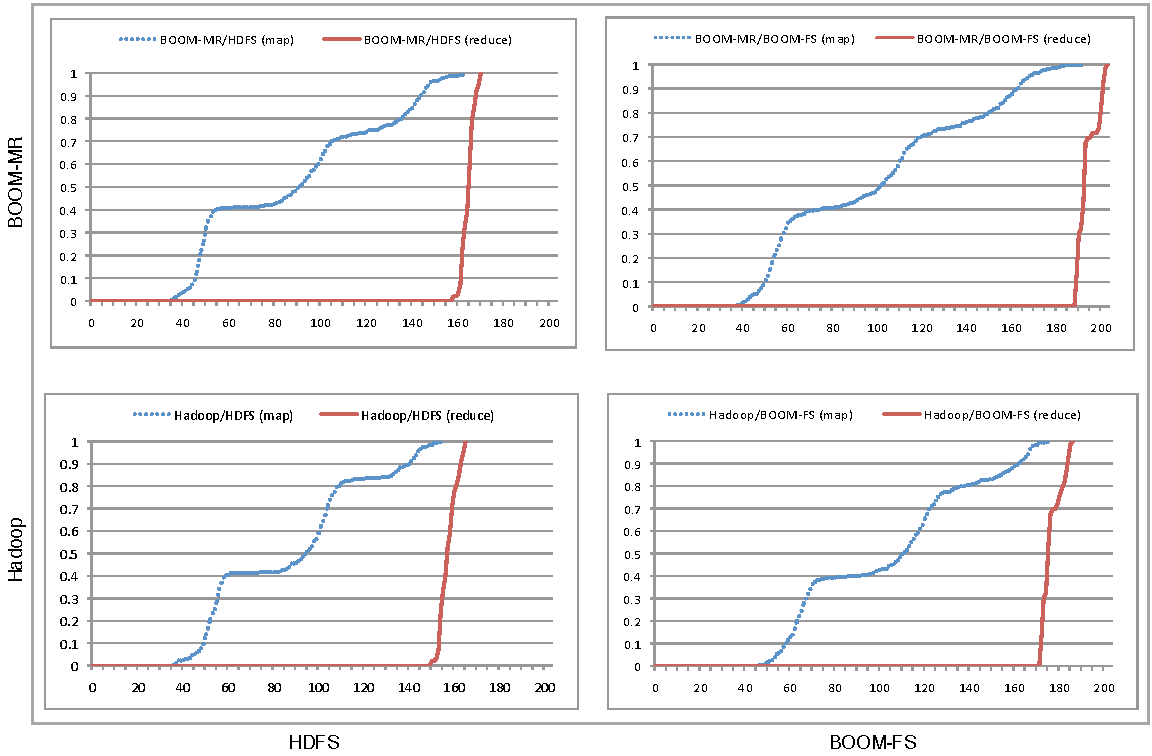
\includegraphics[scale=0.75]{figures/fourgraphs}
\caption{CDFs representing the elapsed time between job startup and task
  completion for both map and reduce tasks, for all combinations of Hadoop and \BOOM-MR
  over HDFS and \BOOM-FS\@.  In each graph, the horizontal axis is
  elapsed time in seconds, and the vertical represents the percentage of tasks completed.}
\label{fig:ec2experiment}
\end{figure*}

While improved performance was not a goal of our work, we wanted to ensure that
the performance of \BOOMA was competitive with Hadoop.  The workload was a
wordcount job on a 30 GB file, using 481 map tasks and 100 reduce tasks.

Figure~\ref{fig:ec2experiment} contains four graphs comparing the performance of
different combinations of Hadoop MapReduce, HDFS, \BOOM-MR, and \BOOM-FS\@. Each
graph reports a cumulative distribution of the elapsed time in seconds from job
startup to map or reduce task completion. The map tasks complete in three
distinct ``waves.'' This is because only 2 $\times$ 100 map tasks can be
scheduled at once. Although all 100 reduce tasks can be scheduled immediately,
no reduce task can finish until all maps have been completed because each reduce
task requires the output of all map tasks.

The lower-left graph describes the performance of Hadoop running on top of HDFS,
and hence serves as a baseline for the subsequent graphs. The upper-left graph
details \BOOM-MR running over HDFS\@. This graph shows that map and reduce task
durations under \BOOM-MR are nearly identical to Hadoop 18.2. The lower-right
and upper-right graphs detail the performance of Hadoop MapReduce and \BOOM-MR
running on top of \BOOM-FS, respectively. \BOOM-FS performance is slightly
slower than HDFS, but remains competitive.


\subsection{LATE policy}

We now compare the behavior of our LATE implementation with the results
observed by Zaharia et al.\ using Hadoop MapReduce.  LATE focuses on how to
improve job completion time by reducing the impact of ``straggler'' tasks.  To
simulate stragglers, we artificially placed additional load on six nodes.  We
ran the same wordcount job on 30 GB of data; using 481 map tasks and 400 reduce
tasks, which produced two distinct ``waves'' of reduce tasks.  We ran each
experiment five times, and report the average over these runs.

Figure~\ref{fig:ec2reduce} shows the reduce task duration CDF for three
different configurations.  The plot labeled ``No Stragglers'' represents normal
load, while the ``Stragglers'' and ``Stragglers (LATE)'' plots describe
performance in the presence in stragglers using the default FCFS policy and the
LATE policy, respectively.  We omit map task durations, because adding
artificial load had little effect on map task execution --- it just resulted in
slightly slower growth from just below 100\% to completion.

\begin{figure*}
\ssp
  \centering
  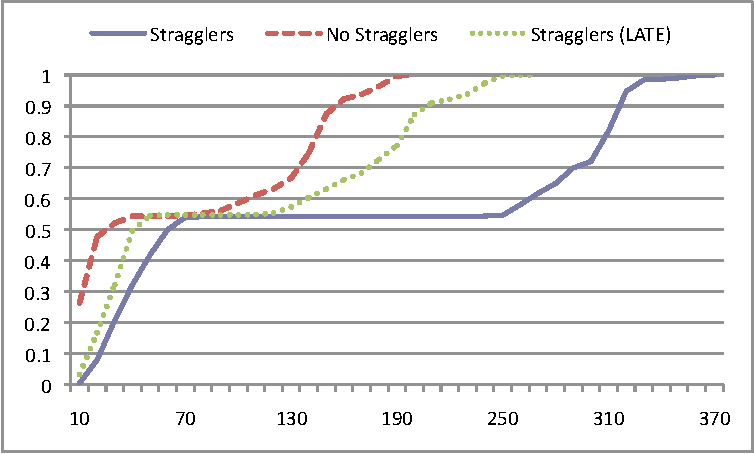
\includegraphics[scale=0.75]{figures/reduce_stragglers}
  \caption{CDF of reduce task duration (secs), with and without stragglers.}
  \label{fig:ec2reduce}
\end{figure*}

The 200 reduce tasks were scheduled concurrently with the map step.  This first
wave of reduce tasks cannot enter the reduce phase until all the map tasks have
completed, which increased their duration, and resulted in the large runtime
durations indicated in the right portion of the graph.  The second wave of 200
reduce tasks did not experience this delay due to unfinished map work since
these reduce tasks were scheduled after all map tasks had finished.  The second
wave of reduce tasks are reported in the left portion of the graph.
Consequently, stragglers had less of an impact on the second wave of reduce
tasks since fewer resources (i.e., no map work) were being consumed.
Figure~\ref{fig:ec2reduce} shows this effect, and also demonstrates how the
LATE implementation in {\BOOMA} handles stragglers much more effectively than
the default Hadoop policy.  This echoes the results reported by Zaharia et
al.~\cite{zaharia-late}

\section{Related Work}
\label{ch:boom:sec:relwork}

Declarative and data-centric languages have traditionally been considered useful
in very few domains, but things have changed substantially in recent years.
MapReduce~\cite{mapreduce-osdi} has popularized functional dataflow programming
with new audiences in computing.  Also, a surprising breadth of recent research
projects have proposed and prototyped declarative languages, including overlay
networks~\cite{p2:sosp}, three-tier web services~\cite{hilda}, natural language
processing~\cite{dyna}, modular robotics~\cite{meld}, video games~\cite{cornellgames}, 
file system metadata analysis~\cite{wiscfsck}, and compiler analysis~\cite{bddbddb}.

Most of the languages cited above are declarative in the same sense as SQL: they are 
based in first-order logic. Some --- notably MapReduce, but also SGL~\cite{cornellgames} --- are
algebraic or dataflow languages, used to describe the composition of operators that produce and 
consume sets or streams of data.  Although arguably imperative, they are far closer to logic languages 
than to traditional imperative languages like Java or C, and are often amenable to set-oriented optimization 
techniques developed for declarative languages~\cite{cornellgames}. Declarative and dataflow languages 
can also share the same runtime, as demonstrated by recent integrations of MapReduce and SQL
in Hive~\cite{hive-vldb}, DryadLINQ~\cite{DryadLINQ}, HadoopDB~\cite{hadoopdb}, and products from vendors 
such as Greenplum and Aster.

Concurrent with our work, the Erlang language was used to implement a simple MapReduce framework called 
Disco~\cite{disco} and a transactional DHT called Scalaris with Paxos support~\cite{scalaris}. Philosophically, Erlang 
revolves around concurrent {\em actors}, rather than data. A closer comparison of actor-oriented and data-centric design 
styles is beyond the scope of this dissertation, but an interesting topic for future work.

\section{Summary}
\label{ch:boom:sec:conclusion}

The initial version of \BOOM-MR required one person-month of development time
and an additional two person-months debugging and tuning \BOOM-MR's performance
for large jobs.  The final version of \BOOM-MR contained declarative
specifications for the core task scheduler (9 rules), the speculative task
scheduler (5 rules), recovery from failed tasks (3 rules), and maintenance of
various job and task related statistics (5 rules).  In total, \BOOM-MR
consisted of 22 \OVERLOG rules in 156 lines of code, and 1269 lines of Java.
\BOOM-MR was based on Hadoop version 18.2; we estimate that we removed 6,573
lines of code (out of 88,863) from the \ol{org.apache.hadoop.mapred} Hadoop
package.  In many fewer lines of code and development time, we were able to
achieve performance characteristics that were competitive to stock Hadoop.

%For this ``porting'' exercise, it was handy to leverage \JOL's Java interfaces
%and draw the Java/\OVERLOG boundaries flexibly.  This allowed us to focus on
%porting the more interesting Hadoop logic into \OVERLOG, while avoiding ports of
%relatively mechanical details.  For example, we chose to leave the data
%representation of the {\em jobConf} as a Java object rather than flatten it
%into a relation because it had no effect on the scheduling logic.

In the end, we found that scheduling policies were a good fit for a declarative
language like \OVERLOG.  In retrospect, this is because scheduling can be
decomposed into two tasks: {\em monitoring} the state of a system and applying
{\em policies} for how to react to changes to that state.  Monitoring is
well-handled by \OVERLOG: we found that the statistics about {\TT} state
required by the LATE policy are naturally realized as aggregate functions, and
\JOL took care of automatically updating those statistics as new messages from
{\TT}s arrived.  In the next chapter, we will look at importing statistics
taken from the output of a MapReduce job that is continuously monitoring
machine and process level statistics.  Once these near real-time monitoring
statistics have been imported into \JOL, we can build some very interesting
scheduling policies around them.

It is also unsurprisingly that a logic language should be well-suited to
specifying policy.  We found the \BOOM-MR scheduler much simpler to extend and
modify than the original Hadoop Java code, as demonstrated by our experience
with LATE\@.  Informally, the \OVERLOG code in \BOOM-MR seems about as complex
as it should be: Hadoop's MapReduce task coordination logic is a simple and
clean design, and the compactness of \BOOM-MR reflects that simplicity
appropriately.  The extensibility of \BOOM-MR benefited us when we extended the
MapReduce batch-oriented model to one that pipelined data between operators
(Chapter~\ref{ch:hop}); supporting both online aggregation~\cite{onlineagg} and
stream processing~\cite{stream} jobs.  
%Pipelining MapReduce required a more
%aggressive operator coscheduling policy that we captured in a few extra
%\OVERLOG rules, beyond those discussed here.


\chapter[MapReduce Online]{MapReduce Online}
\label{ch:hop}

MapReduce is typically applied to large batch-oriented computations that do not
require any real-time completion constraints.  The Google MapReduce
framework~\cite{mapreduce-osdi} and open-source Hadoop system reinforce this
usage model through a batch-processing implementation strategy: the entire
output of each map and reduce task is {\em materialized} to a local file
before it can be consumed by the next stage.  Materialization allows for a
simple and elegant checkpoint/restart fault-tolerance mechanism that is
critical in large deployments, which have a high probability of slowdowns or
failures at worker nodes.  However, batch-processing is not a requirement for
fault-tolerance.  Moreover, batch-processing prevents many online data
processing strategies~\cite{onlineagg, borealis, stream, tcq-cidr} and its
aggressive materialization strategy can be costly in terms of efficiency e.g.,
energy~\cite{yanpei}.

In this chapter, we propose an alternative MapReduce architecture in which
intermediate data is {\em pipelined} between operators, while preserving the
programming interfaces and fault-tolerance properties of previous MapReduce
frameworks.  To validate our design, we developed the Hadoop Online Prototype
(HOP): a pipelined version of Hadoop.\footnote{The source code for HOP can be
downloaded from \url{http://code.google.com/p/hop/}}

Pipelining provides several important advantages to a MapReduce
framework, but also raises new design challenges. We highlight the
potential benefits first:
\begin{itemize}
\ssp
\item
  Since reducers begin processing data as soon as it is produced by mappers,
  they can generate and refine an approximation of their final answer during the
  course of execution. This technique, known as {\em online
    aggregation}~\cite{onlineagg}, can provide initial estimates of results
  several orders of magnitude faster than the final result.  We
  describe how we adapted online aggregation to our pipelined MapReduce
  architecture in Chapter~\ref{ch:hop:sec:online}.

\item
  Pipelining widens the domain of problems to which MapReduce can be applied. In
  Chapter~\ref{ch:hop:sec:continuous}, we show how HOP can be used to support
  {\em continuous queries}: MapReduce jobs that run continuously, accepting new
  data as it arrives and analyzing it immediately. This allows MapReduce to be
  used for applications such as event monitoring and stream processing.

\item
  Pipelining delivers data to downstream operators more promptly, which can
  increase opportunities for parallelism, improve utilization, and reduce
  response time. A thorough performance study is a topic for future work;
  however, in Chapter~\ref{ch:hop:sec:perf} we present some initial performance
  results which demonstrate that pipelining can reduce job completion times by
  up to 25\% in some scenarios.
\end{itemize}

We develop the design of HOP's pipelining scheme in
Chapter~\ref{ch:hop:sec:pipelining}, keeping the focus on traditional batch
processing tasks.  Pipelining raises several design challenges.  First,
Google's attractively simple MapReduce fault-tolerance mechanism is predicated
on the materialization of intermediate state.  In Chapter~\ref{ch:hop:sec:ft},
we show that fault-tolerance can coexist with pipelining, by allowing producers
to periodically ship data to consumers in parallel with data materialization.
A second challenge arises from the greedy communication implicit in pipelines,
which is at odds with batch-oriented optimizations supported by ``combiners'':
map-side code that reduces network utilization by performing pre-aggregation
before communication.  We discuss how the HOP design addresses this issue in
Chapter~\ref{ch:hop:sec:intra-pipe}.  Finally, pipelining requires that
producers and consumers are co-scheduled intelligently.  In
Chapter~\ref{ch:hop:sec:jolport}, we discuss some declarative scheduling
policies that try to fill the pipeline early --- by scheduling downstream
operators first --- and enforce a complete pipeline for continuous queries.

The remaining portions of this chapter focus on applications of HOP and
scheduling policies related to those applications.  In
Chapter~\ref{ch:hop:sec:online}, we show how HOP can support online aggregation
for long-running jobs and illustrate the potential benefits of that interface
to MapReduce programmers.  Chapter~\ref{ch:hop:sec:continuous} describes our
support for continuous MapReduce jobs over data streams and demonstrate an
example of a near-real-time cluster monitoring application.  In
Chapter~\ref{ch:hop:sec:boom}, we return to the topic of scheduling to address
the new challenges raised by these HOP applications.
Chapter~\ref{ch:hop:sec:jolport} describes our port of the \BOOM-MR declarative
scheduler to HOP and some new \OVERLOG scheduling policies that deal with
online aggregation and continuous jobs.  Chapter~\ref{ch:hop:sec:jolmonitor}
introduces a new speculation policy based on statistics collected by a
(continuous) MapReduce monitoring job described in
Chapter~\ref{ch:hop:sec:monitor}.  Finally, Chapter~\ref{ch:hop:sec:relwork}
concludes with some related work.

\section{Pipelined MapReduce}
\label{ch:hop:sec:pipelining}

We begin with a description of our Hadoop extensions that support pipelining
between tasks (Chapter~\ref{ch:hop:sec:intra-pipe}) and jobs
(Chapter~\ref{ch:hop:sec:inter-pipe}).  We describe how our design supports
fault-tolerance (Chapter~\ref{ch:hop:sec:ft}) and compare the performance of HOP
under both pipelining and blocking execution modes
(Chapter~\ref{ch:hop:sec:perf}).

%\begin{figure}[t]
%  \centering
%  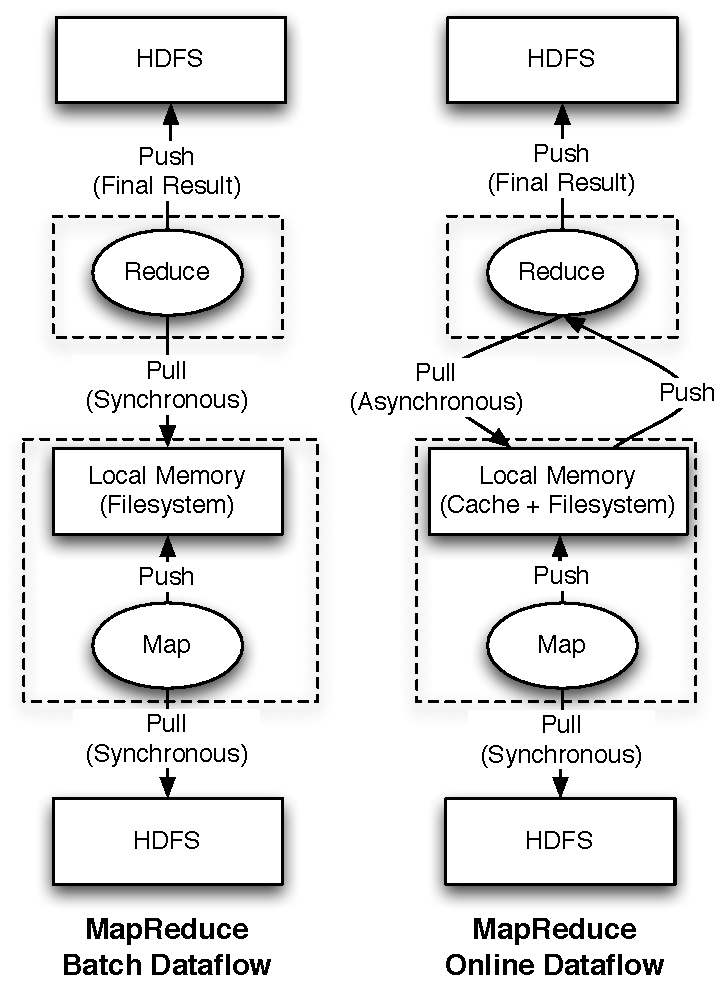
\includegraphics[width=0.90\linewidth]{figures/dataflow_arch.pdf}
%  \caption{Hadoop dataflow for batch (left) and pipelined (right) processing of MapReduce computations.}
%  \label{ch:hop:fig:pipeline}
%\end{figure}
%Figure~\ref{ch:hop:fig:pipeline} depicts the dataflow of two MapReduce
%configurations.  The dataflow on the left describes the materialization
%approach followed by stock Hadoop, while the dataflow on the right allows
%pipelining.  In the remainder of this section, we present our design and
%implementation for the pipelined Hadoop dataflow.  We describe how our design
%supports fault tolerance (Section~\ref{ch:hop:sec:ft}), and discuss the
%interaction between pipelining and task scheduling
%(Section~\ref{ch:hop:sec:pipeline-sched}).

\subsection{Pipelining Within A Job}
\label{ch:hop:sec:intra-pipe}

As described in Chapter~\ref{ch:hadoop:sec:reducetask}, reduce tasks
traditionally issue HTTP requests to {\em pull} their input from each {\TT}
that hosted a map task belonging to the same job.  A \TT is responsible for
serving these HTTP requests, which could occur long after the map task's
execution.  This means that map task execution is completely decoupled from
reduce task execution.  To support pipelining, we modified the \TT serving
component to {\em push} data to reducers as it is produced by the map tasks,
while still maintaining the decoupling of these two steps.  To give an
intuition for how this works, we begin by describing a straightforward
pipelining design, and then discuss the changes we had to make to achieve good
performance.

\subsubsection{Na\"{\i}ve Pipelining}
\label{ch:hop:sec:naive}

We begin with a na\"{\i}ve implementation that sends data directly from map to
reduce tasks via a TCP socket.  Immediately, this design couples the execution
of map and reduce task executions, forcing us to schedule {\em all} reduce
tasks before any one map task.  Consequently, this design does not scale, most
notably when there is not sufficient reduce task slot capacity, but there are
other ramifications that we discuss here before converging on the true HOP
design.

Recall, that when a client submits a new job to Hadoop, the {\JT} assigns the
map and reduce tasks associated with the job to the available {\TT} slots.  For
purposes of {\em this} discussion, we must assume that there are enough free
slots to assign all reduce tasks in a job.  We modified Hadoop so that each
reduce task contacts every map task upon initiation of the job, and opens a TCP
socket which will be used to pipeline the output of the map function.  As each
map output record is produced, the mapper determines which partition (reduce
task) the record should be sent to, and immediately sends it via the
appropriate socket.

A reduce task accepts the pipelined data it receives from each map task and
stores it in an in-memory buffer, spilling sorted runs of the buffer to disk as
needed. Once the reduce task learns that every map task has completed, it
performs a final merge of all the sorted runs and applies the user-defined
reduce function as normal.

\subsubsection{Refinements}
\label{ch:hop:sec:pipe-refine}

While the algorithm described above is straightforward, it suffers from several
practical problems.  First, it is possible that there will not be enough slots
available to schedule every task in a new job.  Opening a socket between every
map and reduce task also requires a large number of TCP connections.  A simple
tweak to the na\"{\i}ve design solves both problems: if a reduce task has not
yet been scheduled, any map tasks that produce records for that partition
simply write them to disk.  When the map task completes, it registers the output
it was not able to send with the host \TT serving component.  Once the reduce
task is assigned a slot, it can then pull the records from the map task's host
\TT, as in regular Hadoop.  To reduce the number of concurrent TCP connections,
each reducer can be configured to pipeline data from a bounded number of
mappers at once; the reducer will pull data from the remaining map tasks in the
traditional Hadoop manner.

Our initial pipelining implementation suffered from a second problem: the map
function was invoked by the same thread that wrote output records to the
pipeline sockets.  This meant that if a network I/O operation blocked (e.g.,
because the reducer was over-utilized), the mapper was prevented from doing
useful work.  Pipeline stalls should not prevent a map task from making
progress -- especially since, once a task has completed, it frees a {\TT} slot
to be used for other purposes.  We solved this problem by running the map
function in a separate thread that stores its output in an in-memory buffer,
and then having another thread periodically send the contents of the buffer to
the connected reducers.~\footnote{This code was based on the existing Hadoop
SpillThread component, which is responsible for writing map output to disk
concurrently with the ``map function.''}

\subsubsection{Granularity of Map Output}
\label{ch:hop:sec:mapout}

Another problem with the na\"{\i}ve design is that it eagerly sends each record
as soon as it is produced, which prevents the use of map-side combiners.
Imagine a job where the reduce key has few distinct values (e.g., gender), and
the reduce applies an algebraic aggregate function (e.g., count).  As discussed
in Chapter~\ref{ch:hadoop:sec:progmodel}, combiners allow map-side
``pre-aggregation'': by applying a reduce-like function to each distinct key at
the mapper, network traffic can often be substantially reduced.  Eagerly
pipelining each record as it is produced prevents the use of these map-side
combiners.

Another related problem is that eager pipelining moves some of the sorting work
from the mapper to the reducer.  Recall from
Chapter~\ref{ch:hadoop:sec:maptask}, that in the blocking architecture, map
tasks generate sorted spill files: all the reduce task must do is merge
together the pre-sorted map output for each partition.  In the na\"{\i}ve
pipelining design, map tasks send output records as they are generated, so a
reducer (scheduled early) must perform a full external sort.  Because the
number of map tasks typically far exceeds the number of
reduces~\cite{mapreduce-osdi}, moving more work to the reducer increased
response time, as shown in our experiments (Chapter~\ref{ch:hop:sec:perf}).

To avoid a heavy reduce task sort, instead of sending the buffer contents to
reducers directly, we wait for the buffer to grow to a threshold size.  The
mapper then (quick) sorts the output by partition and reduce key, applies the
combiner function, and writes the buffer to disk using the Hadoop spill file
format described in Figure~\ref{ch:hadoop:fig:mapoutput}.  Next, we arranged
for the {\TT} serving component at each node to handle pipelining data to
reduce tasks.  Map tasks register spill files with the {\TT} via
RPCs.~\footnote{We extended the existing RPC Hadoop interface to include
information on individual spill files.  Having the spill files be in the same
format allowed us to reuse much of the stock Hadoop serving code i.e., I/O file
formats/streams.}  If the reducers are able to keep up with the production of
map outputs and the network is not a bottleneck, a spill file will be sent to a
reducer soon after it has been produced (in which case, the spill file is
likely still resident in the map machine's kernel buffer cache).  However, if a
reducer begins to fall behind, the number of unsent spill files will grow.

When a map task generates a new spill file, it first queries the {\TT} for the
number of unsent spill files.  If this number grows beyond a certain threshold
(two unsent spill files in our experiments), the map task does not immediately
register the new spill file with the {\TT}.  Instead, the mapper will
accumulate multiple spill files.  Once the queue of unsent spill files falls
below the threshold, the map task merges and combines the accumulated spill
files into a single file, and then resumes registering its output with the
{\TT}.  This simple flow control mechanism has the effect of {\em adaptively}
moving load from the reducer to the mapper or vice versa, depending on which
node is the current bottleneck.

A similar mechanism is also used to control how aggressively the combiner
function is applied.  The map task records the ratio between the input and
output data sizes whenever it invokes the combiner function.  If the combiner
is effective at reducing data volumes, the map task accumulates more spill
files (and applies the combiner function to all of them) before registering
that output with the {\TT} for pipelining.\footnote{Our current prototype uses
a simple heuristic: if the combiner reduces data volume by $\frac{1}{k}$ on
average, we wait until $k$ spill files have accumulated before registering them
with the {\TT}.  A better heuristic would also account for the computational
cost of applying the combiner function.}

The connection between pipelining and adaptive query processing techniques has
been observed elsewhere (e.g.,~\cite{eddies, bamboo}).  The adaptive scheme
outlined above is relatively simple, but we believe that adapting to feedback
along pipelines has the potential to significantly improve the utilization of
MapReduce clusters.

\subsection{Pipelining Between Jobs}
\label{ch:hop:sec:inter-pipe}

Many practical computations cannot be expressed as a single MapReduce job, and
the outputs of higher-level languages like Pig~\cite{pig-sigmod} typically involve
multiple jobs.  In the traditional Hadoop architecture, the output of each job
is written to HDFS in the reduce step and then immediately read back from HDFS
by the map step of the next job. Furthermore, the {\JT} cannot schedule a
consumer job until the producer job has completed, because scheduling a map task
requires knowing the HDFS block locations of the map's input split.

In our modified version of Hadoop, the reduce tasks of one job can optionally
pipeline their output directly to the map tasks of the next job, sidestepping
the need for expensive fault-tolerant storage in HDFS for what amounts to a
temporary file.  Unfortunately, the computation of the reduce function from the
previous job and the map function of the next job cannot be overlapped: the
final result of the reduce step cannot be produced until all map tasks have
completed, which prevents effective pipelining.  However, we describe later how
online aggregation and continuous query pipelines can publish ``snapshot''
outputs that can indeed pipeline between jobs.

\subsection{Fault Tolerance}
\label{ch:hop:sec:ft}

% nrc: (1) Quantify the overhead added by tracking map task origin (2)
% Did we implement the "don't rerun map task from scratch" idea?

Our pipelined Hadoop implementation is robust to the failure of both
map and reduce tasks. To recover from map task failures, we added
bookkeeping to the reduce task to record which map task produced each
pipelined spill file. To simplify fault-tolerance, the reducer treats
the output of a pipelined map task as ``tentative'' until the {\JT}
informs the reducer that the map task has committed successfully. The
reducer can merge together spill files generated by the same
uncommitted mapper, but will not combine those spill files with the
output of other map tasks until it has been notified that the map task
has committed. Thus, if a map task fails, each reduce task can ignore
any tentative spill files produced by the failed map attempt. The
{\JT} will take care of scheduling a new map task attempt, as in stock
Hadoop. 

If a reduce task fails and a new copy of the task is started, the new
reduce instance must be sent all the input data that was sent to the
failed reduce attempt. If map tasks operated in a purely pipelined
fashion and discarded their output after sending it to a reducer, this
would be difficult. Therefore, map tasks retain their output data on
the local disk for the complete job duration. This allows the map's output to be 
reproduced if any reduce tasks fail. For batch jobs, the key advantage of our architecture is
that reducers are not blocked waiting for the complete output of the
task to be written to disk.

Our technique for recovering from map task failure is straightforward, but
places a minor limit on the reducer's ability to merge spill files. To avoid
this, we envision introducing a ``checkpoint'' concept: as a map task runs, it
will periodically notify the {\JT} that it has reached offset $x$ in its input
split. The {\JT} will notify any connected reducers; map task output that was
produced before offset $x$ can then be merged by reducers with other map task
output as normal. To avoid duplicate results, if the map task fails, the new map
task attempt resumes reading its input at offset $x$. This technique would also
reduce the amount of redundant work done after a map task failure or during
speculative execution of ``backup'' tasks~\cite{mapreduce-osdi}.

\subsection{Performance Evaluation}
\label{ch:hop:sec:perf}

A thorough performance comparison between pipelining and blocking is not the
focus of this work.  However, as future work we plan to investigate a
rule-based (e.g., Evita Raced) optimizer for Hadoop MapReduce that considers
pipelined plans in its search strategy.  Here, we demonstrate that pipelining
can reduce job completion times in some configurations and should be considered
by any such optimizer.

We report performance using both large (512MB) and small (32MB) HDFS block
sizes using a single workload (a wordcount job over randomly-generated text).
Since the words were generated using a uniform distribution, map-side combiners
were ineffective for this workload.  We performed all experiments using
relatively small clusters of Amazon EC2 nodes.  We also did not consider
performance in an environment where multiple concurrent jobs are executing
simultaneously.

\subsubsection{Background and Configuration}

Before diving into the performance experiments, it is important to further
describe the division of labor in a HOP job, which is broken into task phases.
A map task consists of two work phases: {\em map} and {\em sort}.  Much of the
work performed during the job happens in the {\em map} phase, where the map
function is applied to each record in the input and subsequently sent to an
output buffer.  Once the entire input has been processed, the map task enters
the {\em sort} phase, where a final merge sort of all intermediate spill files
is performed before registering the final output with the \TT.  The progress
reported by a map task corresponds to the {\em map} phase, which is overlapped
with many in-memory record buffer sorts and subsequent spills to local files.

A reduce task in HOP is divided into three work phases: {\em shuffle}, {\em
reduce}, and {\em commit}.  In the {\em shuffle} phase, reduce tasks receive
their portion of the output from each map.  In HOP, the {\em shuffle} phase
consumes 75\% of the overall reduce task progress while the remaining 25\% is
allocated to the {\em reduce} and {\em commit} phase.~\footnote{The stock
version of Hadoop divides the reduce progress evenly among the three phases.
We deviated from this approach because we wanted to focus more on the progress
during the {\em shuffle} phase.} In the {\em shuffle} phase, reduce tasks
periodically perform a merge sort on the already received map output.  These
intermediate merge sorts decrease the amount of sorting work performed at the
end of the {\em shuffle} phase.  After receiving its portion of data from all
map tasks, the reduce task performs a final merge sort and enters the {\em
reduce} phase.

By pushing work from map tasks to reduce tasks more aggressively, pipelining
can enable better overlapping of map and reduce computation, especially when
the node on which a reduce task is scheduled would otherwise be underutilized.
However, when reduce tasks are already the bottleneck, pipelining offers fewer
performance benefits, and may even hurt performance by placing additional load
on the reduce nodes.

The {\em sort} phase in the map task minimizes the merging work that reduce
tasks must perform at the end of the {\em shuffle} phase.  When pipelining is
enabled, the {\em sort} phase is avoided since map tasks have already sent some
fraction of the spill files to concurrently running reduce tasks.  Therefore,
pipelining increases the merging workload placed on the reducer.  The adaptive
pipelining scheme described in Chapter~\ref{ch:hop:sec:mapout} attempts to
ensure that reduce tasks are not overwhelmed with additional load.

We used two Amazon EC2 clusters depending on the size of the experiment:
``small'' jobs used 10 worker nodes, while ``large'' jobs used 20.  Each node
was an ``extra large'' EC2 instances with 15GB of memory and four virtual
cores, each running at 2.4GHz with a 2GB L2 cache.

\subsubsection{Small Job Results}

\begin{figure*}[t]
\ssp
\begin{minipage}{0.5\linewidth}
  \centering
        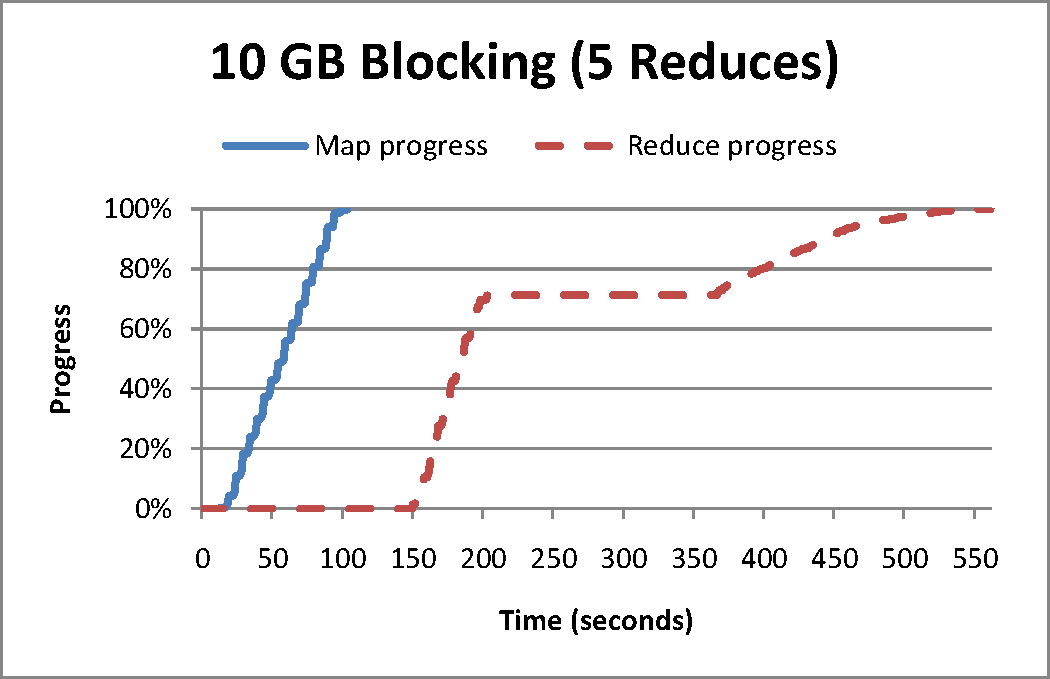
\includegraphics[width=0.90\linewidth]{figures/wc_10gb_20m5r_blocking}
\end{minipage}
\begin{minipage}{0.5\linewidth}
  \centering
        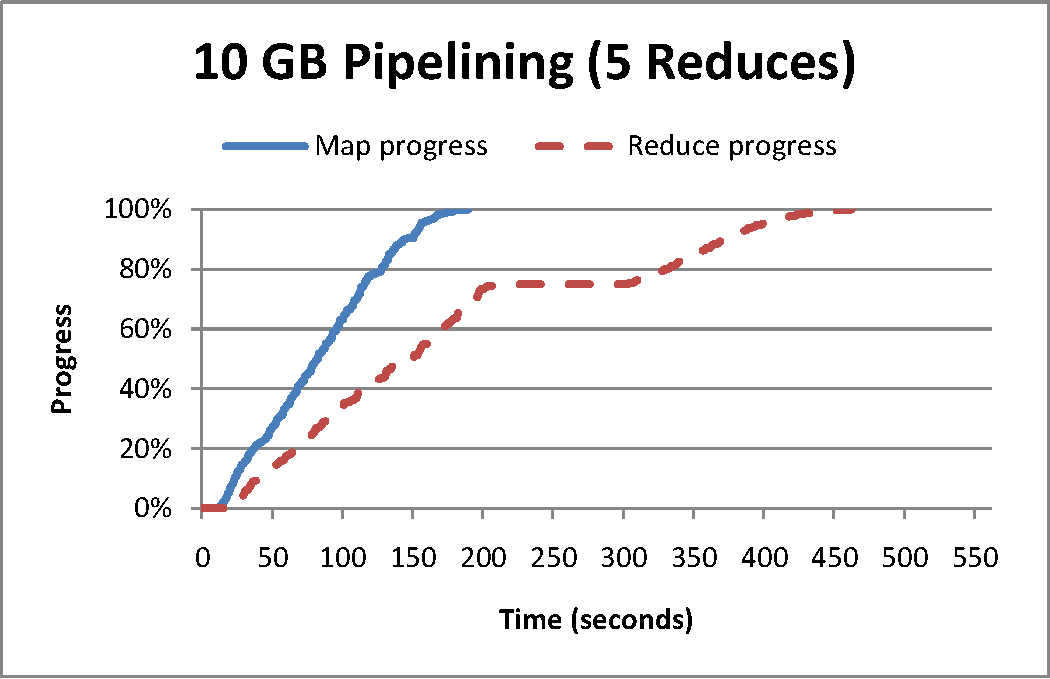
\includegraphics[width=0.90\linewidth]{figures/wc_10gb_20m5r_pipeline}
\end{minipage}
\caption{CDF of map and reduce task completion times for a 10GB wordcount job
  using 20 map tasks and 5 reduce tasks (512MB block size). The total job
  runtimes were 561 seconds for blocking and 462 seconds for pipelining.}
\label{ch:hop:fig:wc1}
\end{figure*}

\begin{figure*}[t]
\ssp
\begin{minipage}{0.5\linewidth}
  \centering
        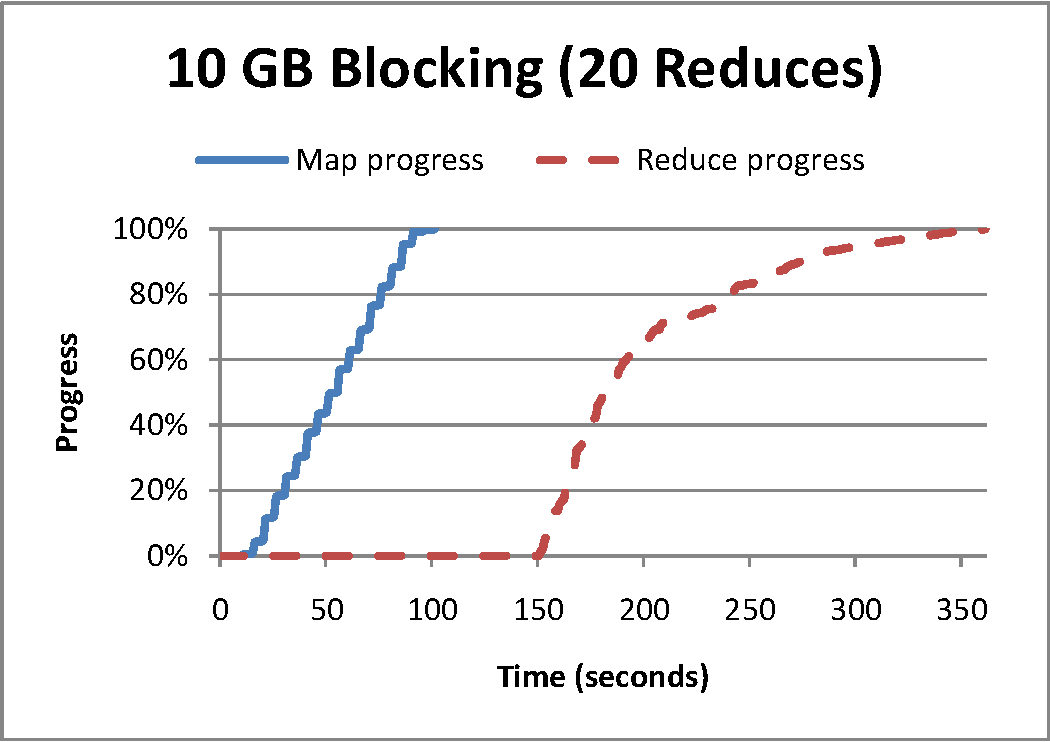
\includegraphics[width=0.88\linewidth]{figures/wc_10gb_20m20r_blocking}
\end{minipage}
\begin{minipage}{0.5\linewidth}
  \centering
        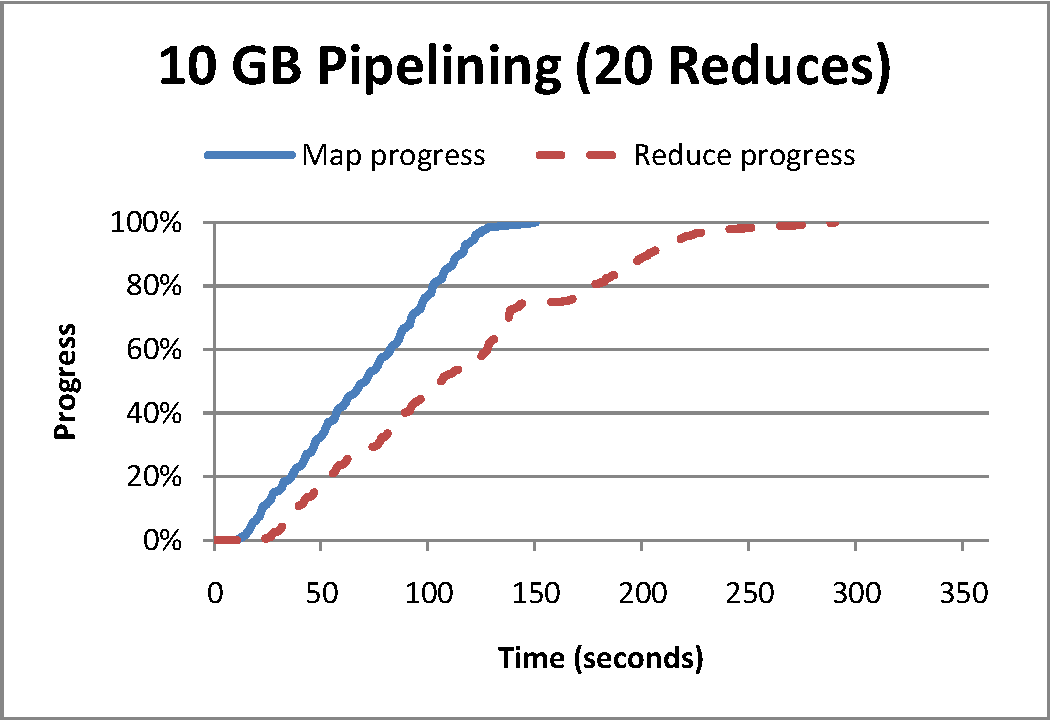
\includegraphics[width=0.90\linewidth]{figures/wc_10gb_20m20r_pipeline}
\end{minipage}
\caption{CDF of map and reduce task completion times for a 10GB wordcount job
  using 20 map tasks and 20 reduce tasks (512MB block size). The total job
  runtimes were 361 seconds for blocking and 290 seconds for pipelining.}
\label{ch:hop:fig:wc2}
\end{figure*}

\begin{figure*}[t]
\ssp
\begin{minipage}{0.5\linewidth}
  \centering
        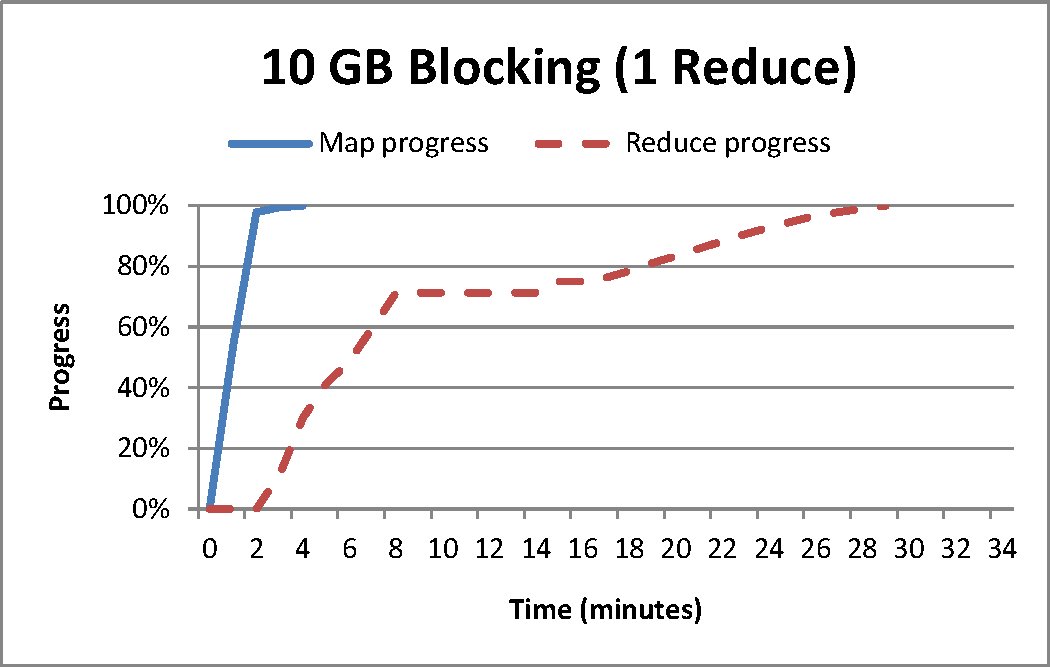
\includegraphics[width=0.95\linewidth]{figures/wc_10gb_20m1r_blocking}
\end{minipage}
\begin{minipage}{0.5\linewidth}
  \centering
        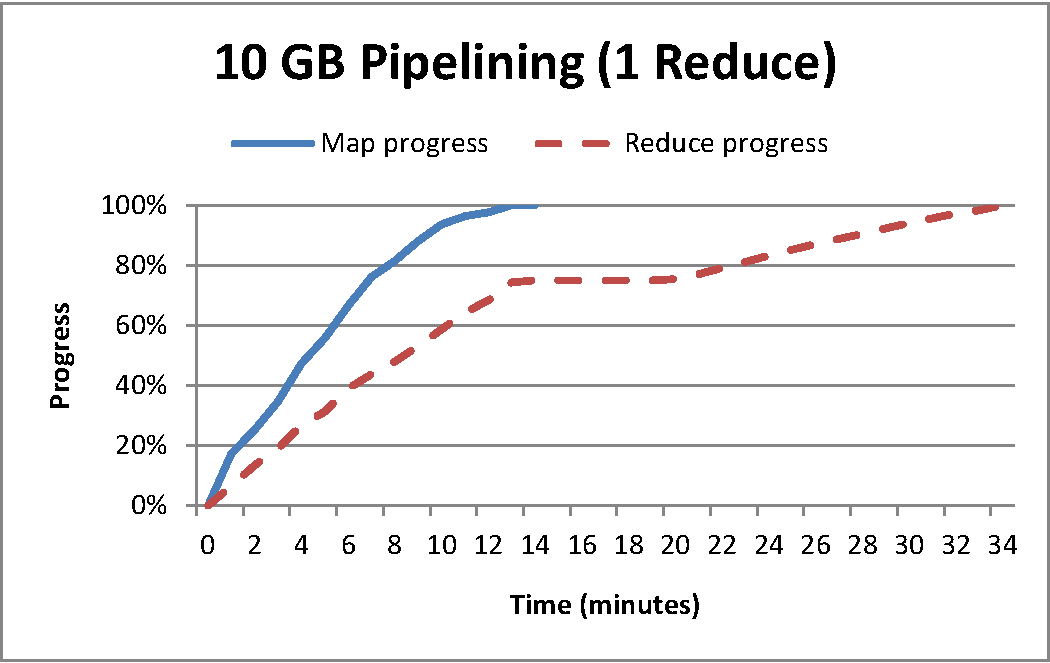
\includegraphics[width=0.95\linewidth]{figures/wc_10gb_20m1r_pipeline}
\end{minipage}
\caption{CDF of map and reduce task completion times for a 10GB wordcount job
  using 20 map tasks and 1 reduce task (512MB block size). The total job
  runtimes were 29 minutes for blocking and 34 minutes for pipelining.}
\label{ch:hop:fig:wc3}
\end{figure*}


Our first experiment focused on the performance of small jobs in an
underutilized cluster.  We ran a 10GB wordcount with a 512MB block size,
yielding 20 map tasks (one per block).  We used 10 worker nodes and configured
each worker to execute at most two map and two reduce tasks simultaneously.  We
ran several experiments to compare the performance of blocking and pipelining
using different numbers of reduce tasks.  For each experiment, we report the
average progress over five separate runs. 

Figure~\ref{ch:hop:fig:wc1} reports the results of a job configured with five
reduce tasks.  A plateau can be seen at 75\% progress for both blocking and
pipelining.  At this point in the job, all reduce tasks have completed the {\em
shuffle} phase; the plateau is caused by the time taken to perform a final
merge of all map output before entering the {\em reduce} phase.  Notice that
the plateau for the pipelining case is shorter.  With pipelining, reduce tasks
receive map outputs much earlier and can begin sorting earlier, thereby
reducing the time required for the final merge.

Figure~\ref{ch:hop:fig:wc2} reports the results with twenty reduce tasks.
Using more reduce tasks decreases the amount of merging that any one reduce
task must perform, which reduces the duration of the plateau at 75\% progress.
In the blocking case, the plateau is practically gone.  However, with
pipelining we still see a small plateau at 75\% that, through further analysis
using \ol{iostat}, can be attributed to extra disk I/Os in the pipelining case.
This extra memory pressure is due to diminished effectiveness of the combiner
in the pipelining case.  Although the response time of pipelining job is better
than the blocking, a job that contains a more effective combiner may be better
executed in blocking mode.

We further note that in both experiments, the map phase finishes faster with
blocking than with pipelining.  This is because pipelining allows reduce tasks
to begin executing earlier and perform more work (sorting and combining);
hence, the reduce tasks compete for resources with the map tasks, causing the
map phase to take slightly longer.  In this case, the increase in map duration
is outweighed by the increase in cluster utilization, resulting in shorter job
completion times: pipelining reduced completion time by 17.7\% with 5 reducers
and by 19.7\% with 20 reducers.

Figure~\ref{ch:hop:fig:wc3} describes an experiment in which we ran a 10GB
wordcount job using a single reduce task.  This caused job completion times to
increase dramatically for both pipelining and blocking, because of the extreme
load placed on the reduce node.  Pipelining delayed job completion by about
17\%, which suggests that our simple adaptive flow control scheme
(Chapter~\ref{ch:hop:sec:mapout}) was unable to move load back to the map tasks
aggressively enough in this (extremely) unbalanced job configuration.

\subsubsection{Large Job Results}

\begin{figure*}[t]
\ssp
\begin{minipage}{0.5\linewidth}
  \centering
        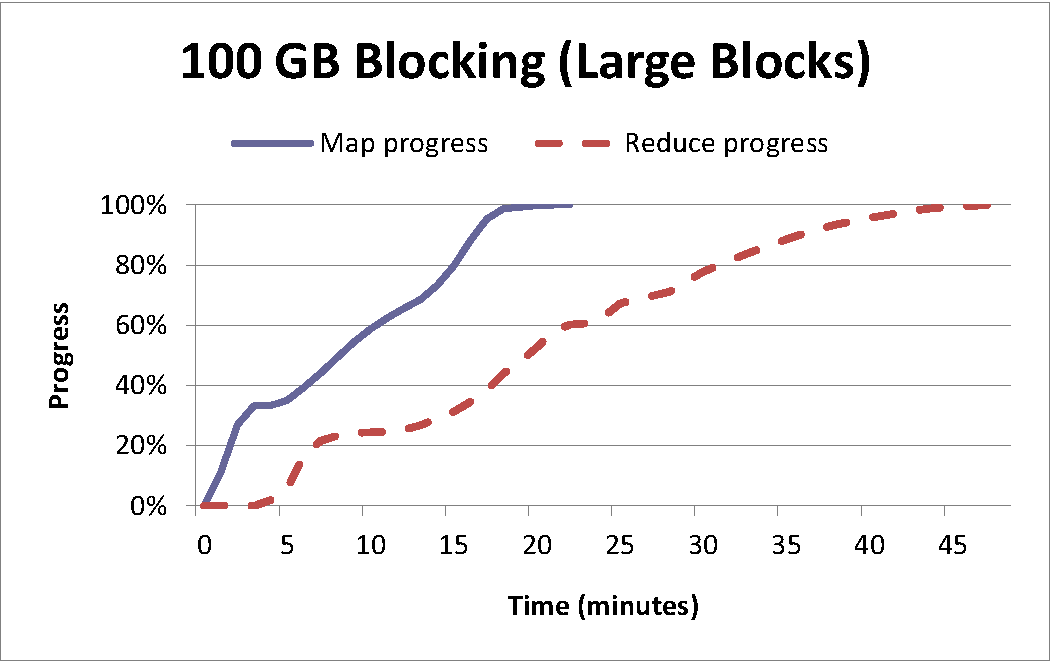
\includegraphics[width=0.95\linewidth]{figures/wc_100gb_240m60r_blocking}
\end{minipage}
\begin{minipage}{0.5\linewidth}
  \centering
        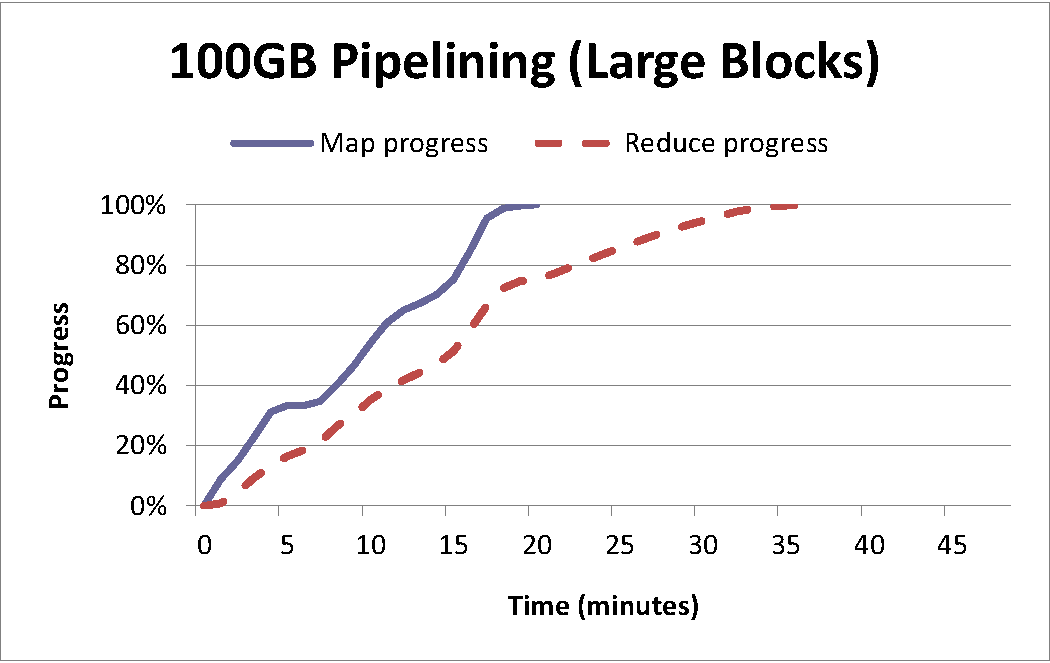
\includegraphics[width=0.95\linewidth]{figures/wc_100gb_240m60r_pipeline}
\end{minipage}
\caption{CDF of map and reduce task completion times for a 100GB wordcount job
  using 240 map tasks and 60 reduce tasks (512MB block size). The total job
  runtimes were 48 minutes for blocking and 36 minutes for pipelining.}
\label{ch:hop:fig:wc4}
\end{figure*}

\begin{figure*}[t]
\ssp
\begin{minipage}{0.5\linewidth}
  \centering
        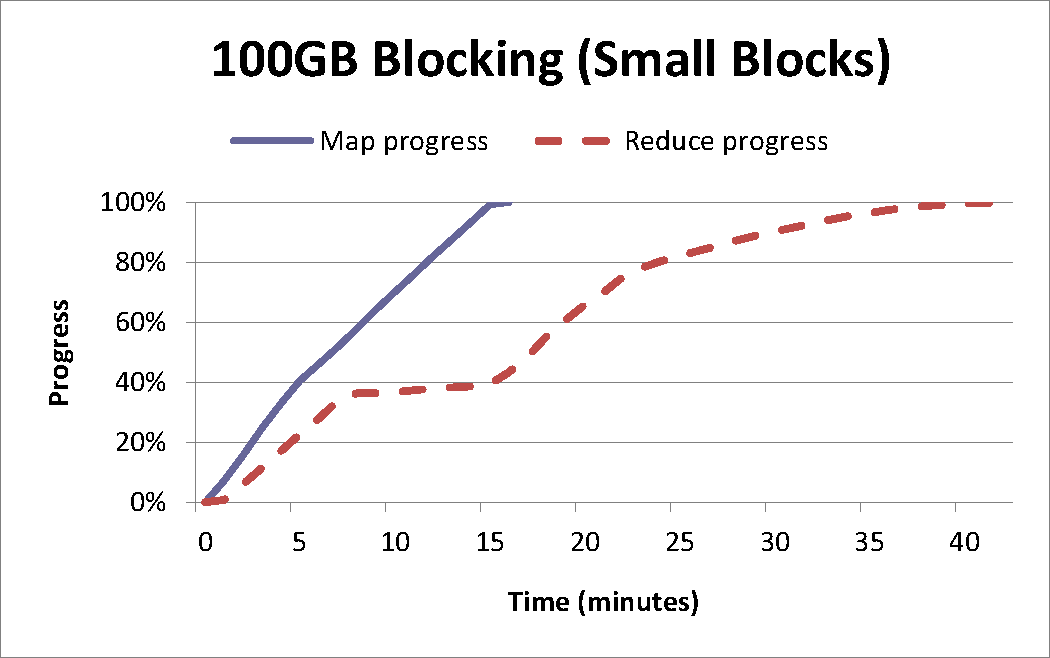
\includegraphics[width=0.95\linewidth]{figures/wc_100gb_3120m60r_blocking}
\end{minipage}
\begin{minipage}{0.5\linewidth}
  \centering
        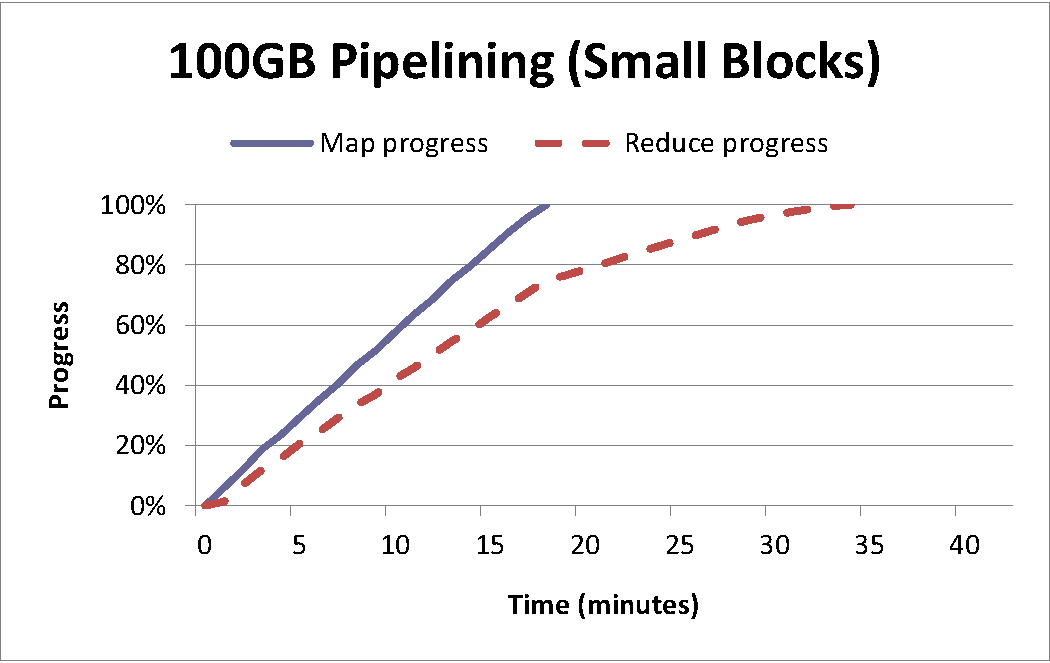
\includegraphics[width=0.95\linewidth]{figures/wc_100gb_3120m60r_pipeline}
\end{minipage}
\caption{CDF of map and reduce task completion times for a 100GB wordcount job
  using 3120 map tasks and 60 reduce tasks (32MB block size). The total job
  runtimes were 42 minutes for blocking and 34 minutes for pipelining.}
\label{ch:hop:fig:wc5}
\end{figure*}

Our second set of experiments focused on the performance of somewhat larger
jobs. We increased the input size to 100GB (from 10GB) and the number of worker
nodes to 20 (from 10). Each worker was configured to execute at most four map
and three reduce tasks, which meant that at most 80 map and 60 reduce tasks
could execute at once. We conducted two sets of experimental runs, each run
comparing blocking to pipelining using either large (512MB) or small (32MB)
block sizes. We were interested in blocking performance with small block sizes
because blocking can effectively emulate pipelining if the block size is small
enough.

Figure~\ref{ch:hop:fig:wc4} reports the performance of a 100GB wordcount job
with 512MB blocks, which resulted in 240 map tasks, scheduled in three waves of
80 tasks each.  The 60 reduce tasks were co-scheduled with the first wave of map
tasks.  In the blocking case, the reduce tasks began working as soon as they
received the output of the first wave, which is why the reduce progress begins
to climb around four minutes (well before the completion of all maps).
Pipelining was able to achieve significantly better cluster utilization, and
hence reduced job completion time by about 25\%.

Comparing the reduce progress in blocking to pipelining, we see that reduce
tasks make more progress during the {\em shuffle} phase when pipelining is
enabled. What is even more interesting is that the {\em reduce} phase is also
shorter in the case of pipelining. The reason for this is subtle; all reduce
tasks enter the {\em phase} around the same time since data is shipped in
smaller increments. In the blocking case, when the final wave of map tasks
finish they all try to send the entire output to reduce tasks at the same time,
which increases the variance on receiving the complete output from all map
tasks. That is, some reduce tasks enter the {\em reduce} phase well in advance
of others.

Figure~\ref{ch:hop:fig:wc5} reports the performance of blocking and pipelining
using 32MB blocks.  While the performance of pipelining remained similar, the
performance of blocking improved considerably, but still trailed somewhat
behind pipelining.  Using block sizes smaller than 32MB did not yield a
significant performance improvement in our experiments.

% \subsection{Discussion}

% As mentioned before, a complete performance evaluation is beyond the scope
% for this paper and we leave such a study for future work.  The focus here was
% to provide some initial insight into the performance benefits of pipelining.
% We also wanted to evaluate the adaptive policy of our pipelining scheme.  To
% this end, we found such a policy paramount in discovering the right amount of
% pipelining to perform based on runtime factors; network capacity and reduce
% task (consumer) load.

%\begin{figure*}[t]
%\begin{minipage}{0.5\linewidth}
%        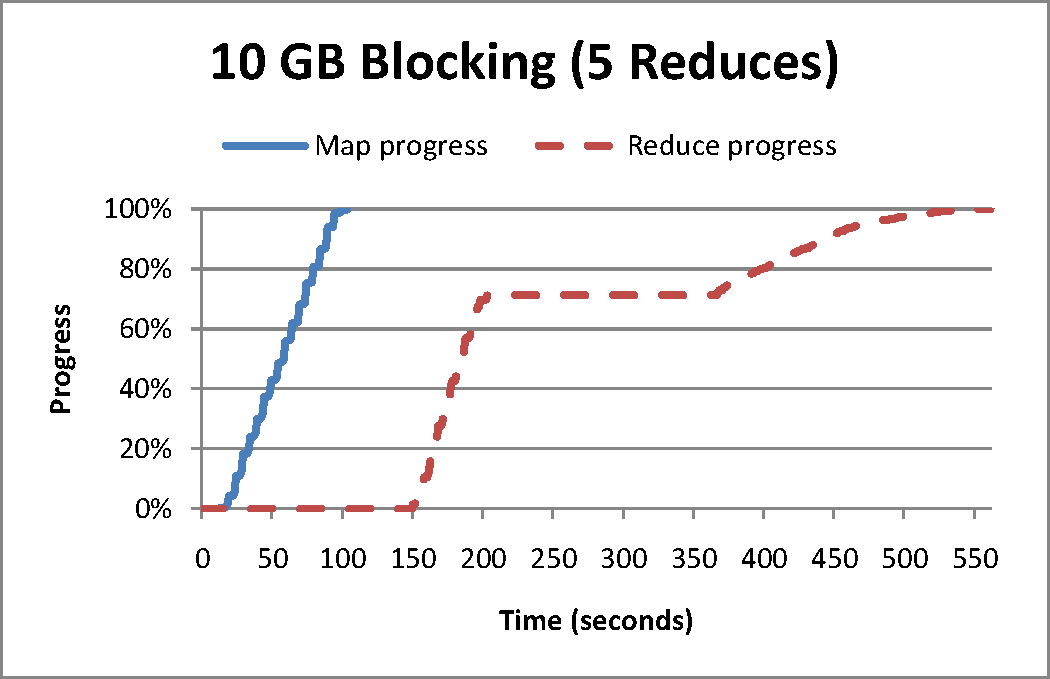
\includegraphics[width=0.95\linewidth]{figures/wc_10gb_20m5r_blocking}
%\end{minipage}
%\begin{minipage}{0.5\linewidth}
%        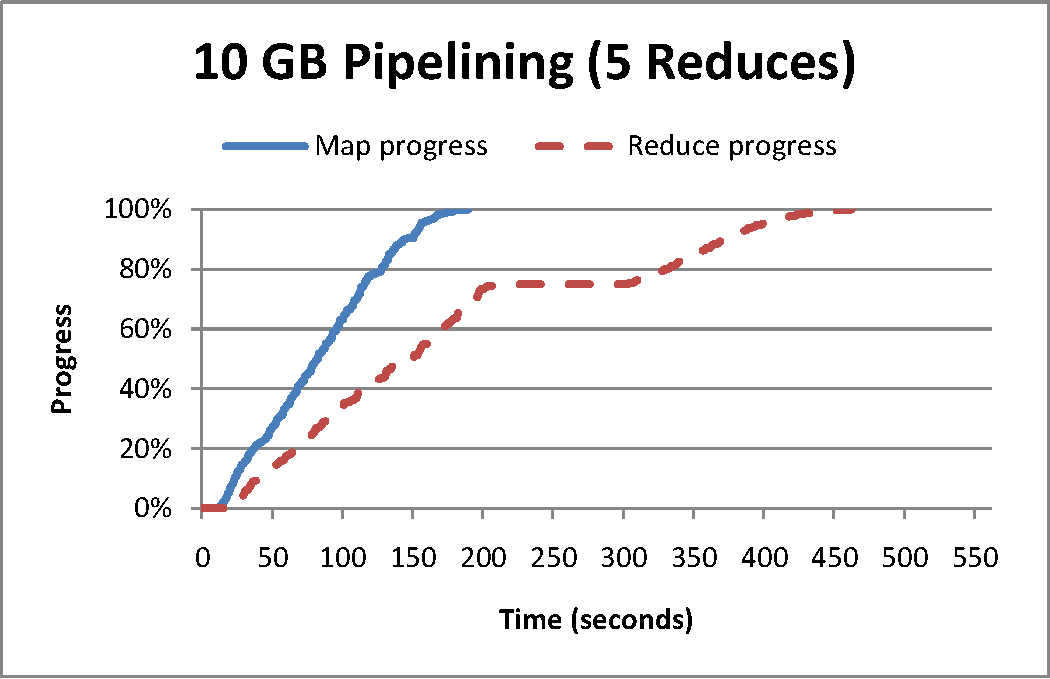
\includegraphics[width=0.95\linewidth]{figures/wc_10gb_20m5r_pipeline}
%\end{minipage}
%\caption{CDF of map and reduce task completion times for a sort job on
%  5.5GB of text extracted from Wikipedia. The total job runtimes were
%  927 seconds for blocking, and 610 seconds for pipelining.}
%\label{fig:sort}
%\end{figure*}

%We conducted a series of performance experiments using a 60-node
%cluster on Amazon EC2. One node executed the Hadoop \JT\ and the HDFS
%\NN, while the remaining 59 nodes served as slaves for running the
%{\TT}s and HDFS {\DN}s. All nodes executed on ``high-CPU medium'' EC2
%instances with 1.7GB of memory and two virtual cores. Each virtual
%core is the equivalent of a 2007-era 2.5Ghz Intel Xeon processor.

%We began by measuring the performance of a simple MapReduce job that
%does not use a combiner. Sorting is commonly used as a benchmark for
%basic MapReduce performance, because of the implicit sort done by the
%reduce phase. We sorted 5.5GB of article text extracted from
%Wikipedia; each word from the text was parsed as a separate
%record. Figure~\ref{fig:sort} describes sort performance on the EC2
%cluster using an HDFS block size of 128MB (yielding 40 map tasks). We
%configured the system to use 59 reducers. In each graph, we give the
%CDF of map and reduce task completion. The left and right graphs
%depict blocking and pipelined performance, respectively.

%Pipelining dominates blocking for this configuration, in part because
%it achieves better cluster utilization: the reduce tasks in the
%blocking job were idle for the first $192$ seconds of the experiment,
%whereas for the pipelined job, reducers began doing useful work within
%$20$ seconds. Note that in a highly-utilized cluster, increased
%pipeline parallelism would not necessarily lead to an improvement in
%total throughput. However, these results suggest that pipelining can
%substantially reduce the response time of an individual job, which can
%often be important (e.g., quickly executing high-priority jobs).


\section{Online Aggregation}
\label{ch:hop:sec:online}

Although MapReduce was originally designed as a batch-oriented system,
it is often used for interactive data analysis: a user submits a job
to extract information from a data set, and then waits to view the
results before proceeding with the next step in the data analysis
process. This trend has accelerated with the development of high-level
query languages that are executed as MapReduce jobs, such as
Hive~\cite{hive-vldb}, Jaql~\cite{jaql}, Pig~\cite{pig-sigmod}, and Sawzall~\cite{sawzall}.

Traditional MapReduce implementations provide a poor interface for interactive
data analysis, because they do not emit any output until the job has been
executed to completion.  In many cases, an interactive user would prefer a
``quick and dirty'' approximation over a correct answer that takes much longer
to compute.  In the database literature, online aggregation has been proposed
to address this problem~\cite{onlineagg}, but the batch-oriented nature of
traditional MapReduce implementations makes these techniques difficult to
apply.  Here, we show how we extended our pipelined Hadoop implementation to
support online aggregation within a single job
(Chapter~\ref{ch:hop:sec:online-single}) and between multiple jobs
(Chapter~\ref{ch:hop:sec:online-multi}).  In
Chapter~\ref{ch:hop:sec:online-eval}, we evaluate online aggregation on two
different data sets, and show that it can yield an accurate approximate answer
long before the job has finished executing.

\subsection{Single-Job Online Aggregation}
\label{ch:hop:sec:online-single}

In HOP, the data records produced by map tasks are sent to reduce tasks shortly
after each record is generated. However, to produce the final output of the job,
the reduce function cannot be invoked until the entire output of every map task
has been produced. We can support online aggregation by simply applying the
reduce function to the data that a reduce task has received so far. We call the
output of such an intermediate reduce operation a {\em snapshot}.

Users would like to know how accurate a snapshot is: that is, how closely a
snapshot resembles the final output of the job.  Accuracy estimation is a hard
problem even for simple SQL queries~\cite{dbo}, and particularly hard for jobs
where the map and reduce functions are opaque user-defined code.  Hence, we
report job {\em progress}, not accuracy: we leave it to the user (or their
MapReduce code) to correlate progress to a formal notion of accuracy.  We
define a simple progress metric later in this chapter.

Snapshots are computed periodically, as new data arrives at each reducer. The
user specifies how often snapshots should be computed, using the progress metric
as the unit of measure. For example, a user can request that a snapshot be
computed when 25\%, 50\%, and 75\% of the input has been seen. The user may also
specify whether to include data from tentative (unfinished) map tasks. This
option does not affect the fault-tolerance design described in
Chapter~\ref{ch:hop:sec:ft}. In the current prototype, each snapshot is stored in a
directory on HDFS\@. The name of the directory includes the progress value
associated with the snapshot. Each reduce task runs independently, and at a
different rate. Once a reduce task has made sufficient progress, it writes a
snapshot to a temporary directory on HDFS, and then atomically renames it to the
appropriate location.

Applications can consume snapshots by polling HDFS in a predictable
location. An application knows that a given snapshot has been
completed when every reduce task has written a file to the snapshot
directory.  Atomic rename is used to avoid applications mistakenly
reading incomplete snapshot files.

Note that if there are not enough free slots to allow all the reduce tasks in a
job to be scheduled, snapshots will not be available for reduce tasks that are
still waiting to be executed. The user can detect this situation (e.g.,\ by
checking for the expected number of files in the HDFS snapshot directory), so
there is no risk of incorrect data, but the usefulness of online aggregation
will be reduced. In the current prototype, we manually configured the cluster to
avoid this scenario. The system could also be enhanced to avoid this pitfall
entirely by optionally waiting to execute an online aggregation job until there
are enough reduce slots available.

\subsubsection{Progress Metric}
\label{ch:hop:sec:online-metric}

Hadoop provides support for monitoring the progress of task executions.  As
each map task executes, it is assigned a {\em progress score} in the range
[0,1], based on how much of its input the map task has consumed.  We reused
this feature to determine how much progress is represented by the current input
to a reduce task, and hence to decide when a new snapshot should be taken.
When the transfer of a spill file to a reduce task occurs, we include a small
amount of meta-data that indicates the map's current progress score, relative
to that spill file.  To compute the overall progress score for a reduce step
snapshot, we take the average of the progress scores associated with each map's
data residing on the reduce task prior to executing the snapshot. 

Note that it is possible to have a map task that has not pipelined {\em any}
output to a reduce task, either because the map task has not been scheduled yet
(there are no free {\TT} slots), the map tasks does not produce any output for
the given reduce task, or because the reduce task has been configured to only
pipeline data from at most $k$ map tasks concurrently.  To account for this, we
need to scale the progress metric to reflect the portion of the map tasks that
a reduce task has pipelined data from: if a reducer is connected to
$\frac{1}{n}$ of the total number of map tasks in the job, we divide the
average progress score by $n$.

This progress metric could easily be made more sophisticated: for example, an
improved metric might include the selectivity ($|output|/|input|$) of each map task, the
statistical distribution of the map task's output, and the effectiveness of each
map task's combine function, if any. 
% We also assume that each map task
% constitutes a random sample from the input file; otherwise, the scale
% factor we use to account for unavailable map input will introduce
% bias. 
Although we have found our simple progress metric to be
sufficient for most experiments we describe below, this clearly
represents an opportunity for future work.

\subsection{Multi-Job Online Aggregation}
\label{ch:hop:sec:online-multi}

Online aggregation is particularly useful when applied to a long-running
analysis task composed of multiple MapReduce jobs.  As described in
Chapter~\ref{ch:hop:sec:inter-pipe}, our version of Hadoop allows the output of
a reduce task to be sent directly to map tasks.  This feature can be used to
support online aggregation for a sequence of jobs.

Suppose that $j_1$ and $j_2$ are two MapReduce jobs, and $j_2$ consumes the
output of $j_1$.  When $j_1$'s reducers compute a snapshot to perform online
aggregation, that snapshot is written to HDFS, and also sent directly to the
map tasks of $j_2$.  The map and reduce steps for $j_2$ are then computed as
normal, to produce a snapshot of $j_2$'s output.  This process can then be
continued to support online aggregation for an arbitrarily long sequence of
jobs.
  
Unfortunately, inter-job online aggregation has some drawbacks.  First, the
output of a reduce function is not ``monotonic'': the output of a reduce
function on the first 50\% of the input data may not be obviously related to
the output of the reduce function on the first 25\%.  Thus, as new snapshots
are produced by $j_1$, $j_2$ must be recomputed from scratch using the new
snapshot.  As with inter-job pipelining (Chapter~\ref{ch:hop:sec:inter-pipe}),
this could be optimized for reduce functions that are declared to be
distributive or algebraic aggregates~\cite{datacube}.

To support fault-tolerance for multi-job online aggregation, we consider three
cases. Tasks that fail in $j_1$ recover as described in Chapter~\ref{ch:hop:sec:ft}.
If a task in $j_2$ fails, the system simply restarts the failed task. Since
subsequent snapshots produced by $j_1$ are taken from a superset of the mapper
output in $j_1$, the next snapshot received by the restarted reduce task in
$j_2$ will have a higher progress score. To handle failures in $j_1$, tasks in
$j_2$ cache the most recent snapshot received by $j_1$, and replace it when they
receive a new snapshot with a higher progress metric. If tasks from both jobs
fail, a new task in $j_2$ recovers the most recent snapshot from $j_1$ that was
stored in HDFS and then wait for snapshots with a higher progress score.

%Figure~\ref{fig:snapshot} depicts an inter-job dataflow for batch
%mode (left) and a dataflow that supports online aggregation
%(right). The batch mode forces jobs to read the final output of other
%jobs from HDFS\@.  

%%We support not only reading snapshots from HDFS but
%%also pipelining snapshots directly to jobs that request them. 
% In addition to reading snapshots from HDFS, we support pipelining
% snapshots directly to the jobs that request them.
% This is
% supported via an asynchronous request call interface exported by
% each reduce task, through which map tasks from other jobs can request
% snapshots and even the final output. The final output is concurrently
% written to HDFS for fault tolerance, unless otherwise specified in the
% configuration of the job.
  
% nrc: Discuss progress metric for inter-job OA
  
\subsection{Evaluation}
\label{ch:hop:sec:online-eval}

\begin{figure}
\ssp
  \centering
    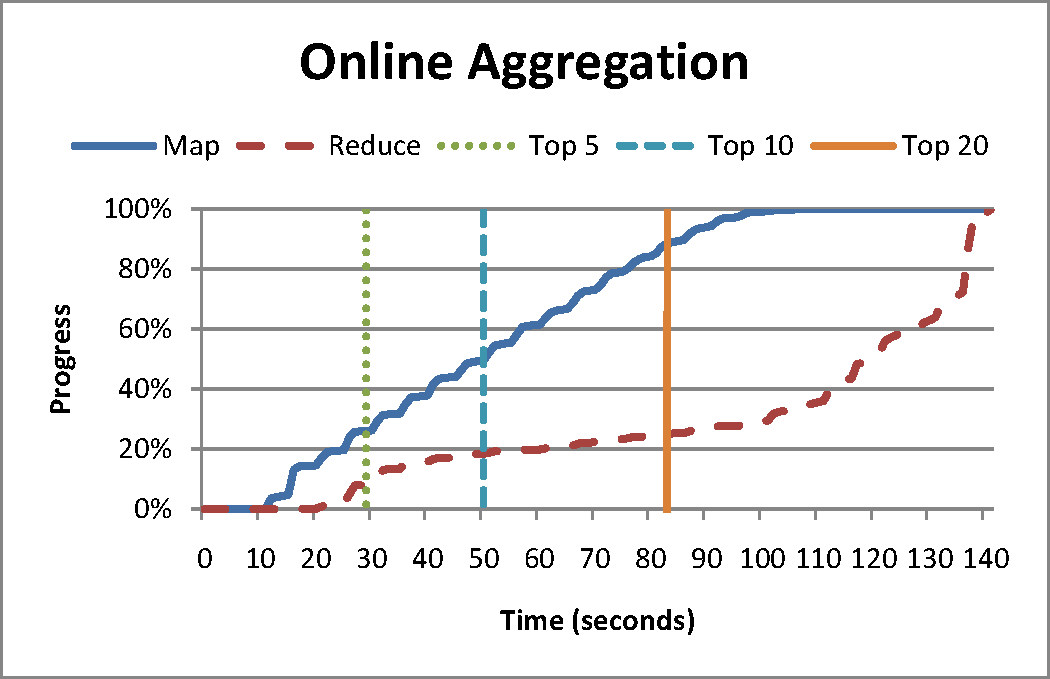
\includegraphics[width=0.7\linewidth]{figures/top100_online_wiki}
    \caption{Top-100 query over 5.5GB of Wikipedia article text. The vertical
      lines describe the increasing accuracy of the approximate answers produced
      by online aggregation.}
\label{fig:topkonlinewiki}
\vspace{-10pt}
\end{figure}

To evaluate the effectiveness of online aggregation, we performed two
experiments on Amazon EC2 using different data sets and query workloads.  In
our first experiment, we wrote a ``Top-$K$'' query using two MapReduce jobs:
the first job counts the frequency of each word and the second job selects the
$K$ most frequent words.  We ran this workload on 5.5GB of Wikipedia article
text stored in HDFS, using a 128MB block size.  We used a 60-node EC2 cluster;
each node was a ``high-CPU medium'' EC2 instance with 1.7GB of RAM and 2
virtual cores.  A virtual core is the equivalent of a 2007-era 2.5Ghz Intel
Xeon processor.  A single EC2 node executed the Hadoop \JT\ and the HDFS \NN,
while the remaining nodes served as slaves for running the {\TT}s and HDFS
{\DN}s.

% To evaluate inter-job dataflow with online aggregation we wrote a
% Top-$K$ query using two MapReduce jobs and executed it on 5.5GB of
% Wikipedia article text. The first job performs a wordcount on the
% words contained in each article.  A reducer from the first job will
% output a list of the Top-$K$ words observed in its partition. The key
% in this output is the word, and the value is the word count. Each map
% task in the subsequent job is assigned to an output from a single
% reduce task. The map function reverses the key-value order, and sends
% that result (sorted by count in descending order) to a single reduce
% task.  The single reduce task merges the sorted lists from each mapper
% and returns the first $K$ words.

% nrc: What does this experiment have to do with online aggregation?
% Figure~\ref{fig:topkwiki} reports the result of a Top-100 query over
% 5.5GB of Wikipedia article text. The left graph represents the
% blocking case as indicated by the idle period in the progress of the
% reduce tasks. The first map tasks finish around 100 seconds into the
% job, which is where the reduce tasks begin to make progress. The
% right graph shows a more balanced load. The reduce tasks
% being receiving mapper output almost immediately following the job
% execution, contributing to the early completion time of the job.

Figure~\ref{fig:topkonlinewiki} shows the results of inter-job online
aggregation for a Top-100 query.  Our accuracy metric for this experiment is
post-hoc --- we note the time at which the Top-$K$ words in the snapshot are
the Top-$K$ words in the final result.  Although the final result for this job
did not appear until nearly the end, we did observe the Top-5, 10, and 20
values at the times indicated in the graph.  The Wikipedia data set was biased
toward these Top-K words (e.g., ``the'', ``is'', etc.), which remained in their
correct position throughout the lifetime of the job.

\subsubsection{Approximation Metrics}

\begin{figure*}[ht]
\ssp
  \centering
  \subfloat[][Relative approximation error over time]{\label{fig:approx-relative}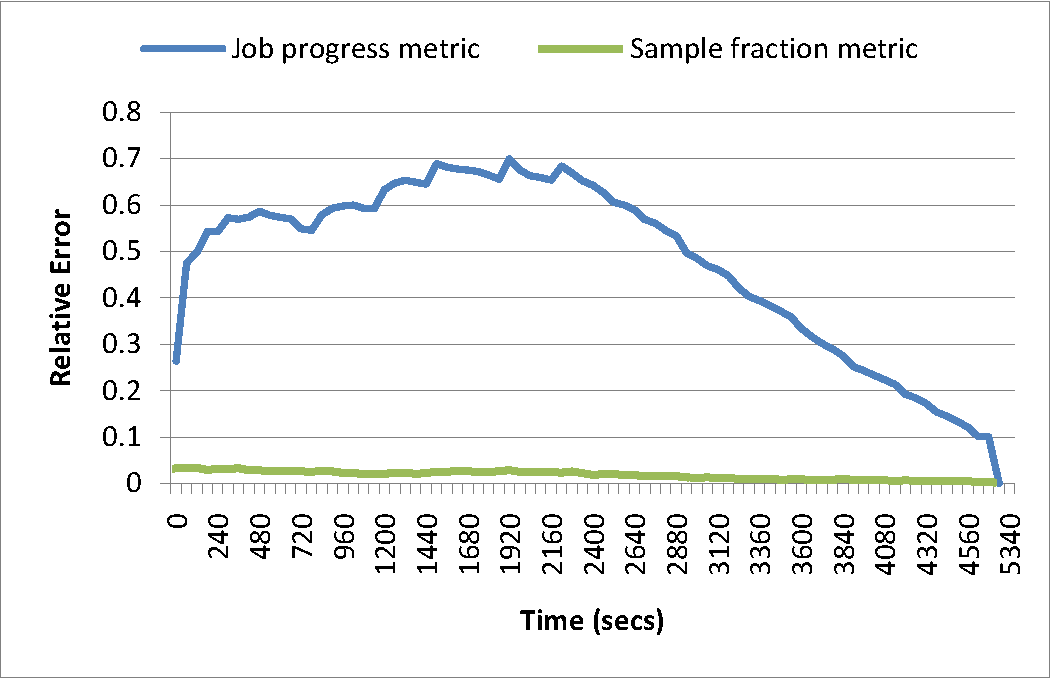
\includegraphics[width=0.48\linewidth]{figures/aprx-click-hour.pdf}}
  \subfloat[][Example approximate answer]{\label{fig:approx-hour}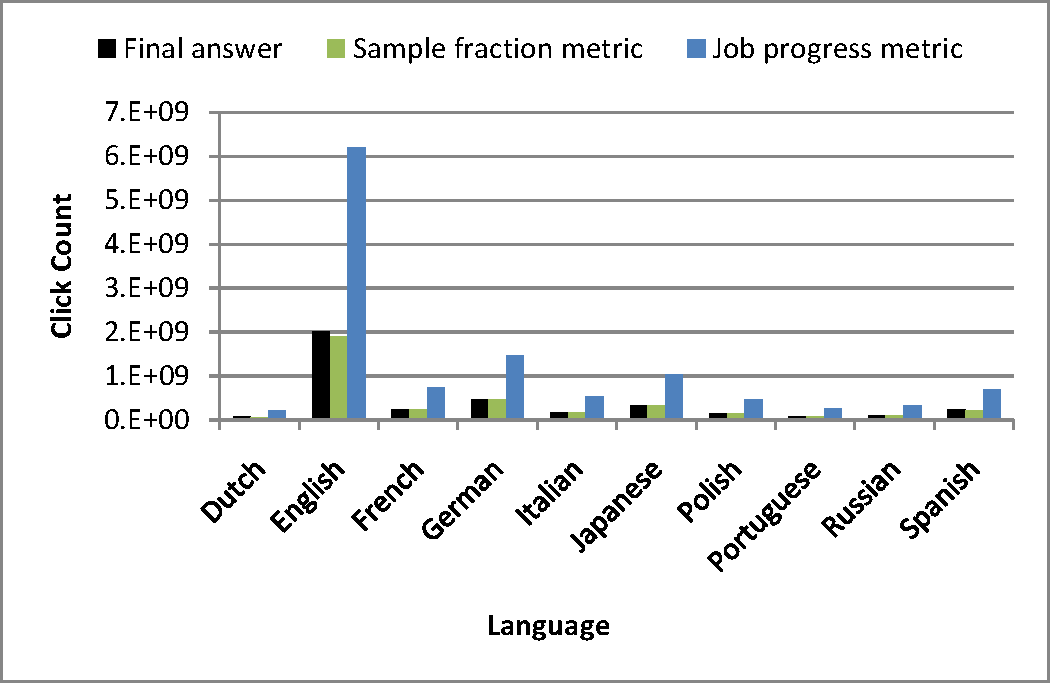
\includegraphics[width=0.48\linewidth]{figures/aprx-click-hour-actual.pdf}}
  \caption{Comparison of two approximation
    metrics. Figure~\protect\subref{fig:approx-relative} shows the relative error for
    each approximation metric over the runtime of the job, averaged over all
    groups. Figure~\protect\subref{fig:approx-hour} compares an example approximate
    answer produced by each metric with the final answer, for each language and for a single hour.}
\label{fig:approx}
\end{figure*}

In our second experiment, we considered the effectiveness of the job progress
metric described in Chapter~\ref{ch:hop:sec:online-metric}. Unsurprisingly, this metric
can be inaccurate when it is used to estimate the accuracy of the approximate
answers produced by online aggregation. In this experiment, we compared the job
progress metric with a simple user-defined metric that leverages knowledge of
the query and data set. HOP allows such metrics, although developing such a
custom metric imposes more burden on the programmer than using the generic
progress-based metric.

We used a data set containing seven months of hourly page view statistics for
more than 2.5 million Wikipedia articles~\cite{wikistats}. This constituted
320GB of compressed data (1TB uncompressed), divided into 5066 compressed
files. We stored the data set on HDFS and assigned a single map task to each
file, which was decompressed before the map function was applied.

We wrote a MapReduce job to count the total number of page views for each
language and each hour of the day. In other words, our query grouped by language
and hour of day, and summed the number of page views that occurred in each
group. To enable more accurate approximate answers, we modified the map function
to include the fraction of a given hour that each record represents. The reduce
function summed these fractions for a given hour, which equated to one for all
records from a single map task. Since the total number of hours was known ahead
of time, we could use the result of this sum over all map outputs to determine
the total fraction of each hour that had been sampled. We call this user-defined
metric the ``sample fraction.''

To compute approximate answers, each intermediate result was scaled up using two
different metrics: the generic metric based on job progress and the sample
fraction described above. Figure~\ref{fig:approx-relative} reports the relative
error of the two metrics, averaged over all groups. Figure~\ref{fig:approx-hour}
shows an example approximate answer for a single hour using both metrics
(computed two minutes into the job runtime). This figure also contains the final
answer for comparison. Both results indicate that the sample fraction metric provides a
much more accurate approximate answer for this query than the progress-based
metric.

Job progress is clearly the wrong metric to use for approximating the final
answer of this query. The primary reason is that it is too coarse of a
metric. Each intermediate result was computed from some fraction of each
hour. However, the job progress assumes that this fraction is uniform across all
hours, when in fact we could have received much more of one hour and much less
of another. This assumption of uniformity in the job progress resulted in a
significant approximation error. By contrast, the sample fraction scales the
approximate answer for each group according to the actual fraction of data seen for
that group, yielding much more accurate approximations.

\section{Continuous Queries}
\label{ch:hop:sec:continuous}

MapReduce is often used to analyze streams of constantly-arriving
data, such as URL access logs~\cite{mapreduce-osdi} and system console
logs~\cite{sosp-mining}. Because of traditional constraints on MapReduce, this 
is done in large batches that can only provide periodic views of activity.
This introduces
significant latency into a data analysis process that ideally should run in 
near-real time. It is also
potentially inefficient: each new MapReduce job does not have access
to the computational state of the last analysis run, so this state
must be recomputed from scratch. The programmer can manually save the
state of each job and then reload it for the next analysis operation,
but this is labor-intensive.

Our pipelined version of Hadoop allows an alternative architecture:
MapReduce jobs that run {\em continuously}, accepting new data as it
becomes available and analyzing it immediately. This allows for near-real-time
analysis of data streams, and thus
allows the MapReduce programming model to be applied to domains such
as environment monitoring and real-time fraud detection.

In this section, we describe how HOP supports continuous MapReduce
jobs, and how we used this feature to implement a rudimentary
cluster monitoring tool.

\subsection{Continuous MapReduce Jobs}
A bare-bones implementation of continuous MapReduce jobs is easy to
implement using pipelining. No changes are needed to implement
continuous map tasks: map output is already delivered to the
appropriate reduce task shortly after it is generated. We added an
optional ``flush'' API that allows map functions to force their current
output to reduce tasks. When a reduce task is unable to accept such data, the mapper framework
stores it locally and sends it at a later time. 
With proper scheduling of reducers, this API allows a map task to ensure that an output record is promptly sent to the appropriate
reducer.

To support continuous reduce tasks, the user-defined reduce function
must be periodically invoked on the map output available at that
reducer. Applications will have different requirements for how
frequently the reduce function should be invoked; possible choices
include periods based on wall-clock time, logical time (e.g., the
value of a field in the map task output), and the number of input rows
delivered to the reducer. The output of the reduce function can be
written to HDFS, as in our implementation of online
aggregation. However, other choices are possible; our prototype system
monitoring application (described below) sends an alert via email if
an anomalous situation is detected.

In our current implementation, the number of map and reduce tasks is
fixed, and must be configured by the user. This is clearly
problematic: manual configuration is error-prone, and many stream
processing applications exhibit ``bursty'' traffic patterns, in which
peak load far exceeds average load. In the future, we plan to add
support for elastic scaleup/scaledown of map and reduce tasks in
response to variations in load.

\subsubsection{Fault Tolerance}
In the checkpoint/restart fault-tolerance model used by Hadoop, mappers retain
their output until the end of the job to facilitate fast recovery from reducer
failures. In a continuous query context, this is infeasible, since mapper
history is in principle unbounded.  However, many continuous reduce functions
(e.g., 30-second moving average) only require a suffix of the map output stream.
This common case can be supported easily, by extending the \JT\ interface to
capture a rolling notion of reducer consumption.  Map-side spill files are
maintained in a ring buffer with unique IDs for spill files over time. When a
reducer commits an output to HDFS, it informs the \JT\ about the {\em run} of
map output records it no longer needs, identifying the run by spill file IDs and
offsets within those files.  The \JT\ can then tell mappers to garbage collect
the appropriate data.

In principle, complex reducers may depend on very long (or infinite) histories of map records to accurately reconstruct their internal state.  In that case, deleting spill files
from the map-side ring buffer will result in potentially inaccurate recovery after faults.  Such scenarios can be handled by having reducers checkpoint internal state to HDFS, along with markers for the mapper offsets at which the internal state was checkpointed.  The MapReduce framework can be extended with APIs to help with state serialization and offset management, but it still presents a programming burden on the user to correctly identify the sensitive internal state.  That burden can be avoided by more heavyweight process-pair 
techniques for fault-tolerance, but those are quite complex and use significant resources~\cite{flux-ft}.  In our work to date we have focused on cases where reducers can be recovered from a reasonable-sized history at the mappers, favoring minor extensions to the simple fault-tolerance approach used in Hadoop.

\subsection{Prototype Monitoring System}
\label{ch:hop:sec:monitor}

Our monitoring system is composed of {\em agents} that run on each monitored
machine and record statistics of interest (e.g., load average, I/O operations
per second, etc.). Each agent is implemented as a continuous map task: rather
than reading from HDFS, the map task instead reads from various system-local
data streams (e.g., \texttt{/proc}).

Each agent forwards statistics to an {\em aggregator} that is implemented as a
continuous reduce task. The aggregator records how agent-local statistics evolve
over time (e.g., by computing windowed-averages), and compares statistics
between agents to detect anomalous behavior. Each aggregator monitors the agents
that report to it, but might also report statistical summaries to another
``upstream'' aggregator. For example, the system might be configured to have an
aggregator for each rack and then a second level of aggregators that compare
statistics between racks to analyze datacenter-wide behavior.

\subsubsection{Evaluation}
\begin{figure}[t]
\ssp
  \centering
  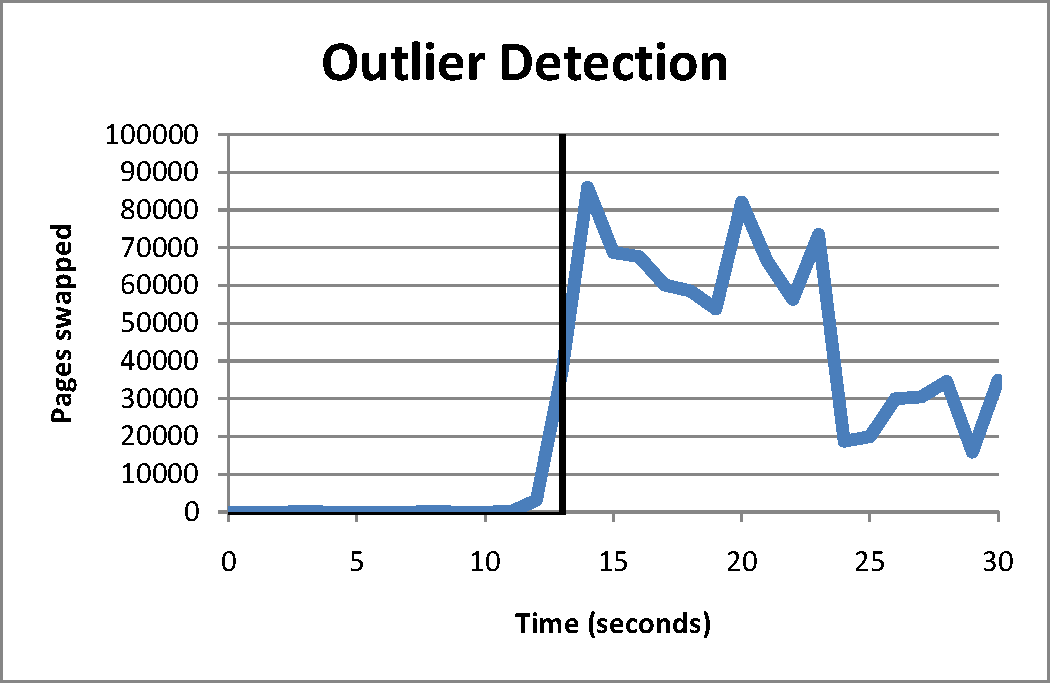
\includegraphics[scale=0.6]{figures/continue.pdf}
  \caption{Number of pages swapped over time on the thrashing host, as reported
    by \texttt{vmstat}.  The vertical line indicates the time at which the alert
    was sent by the monitoring system.}
\label{fig:outlier}
\end{figure}

To validate our prototype system monitoring tool, we constructed a
scenario in which one member of a MapReduce cluster begins thrashing
during the execution of a job. Our goal was to test how quickly our
monitoring system would detect this behavior. The basic mechanism is
similar to an alert system one of the authors implemented at an
Internet search company.

We used a simple load metric (a linear combination of CPU utilization,
paging, and swap activity). The continuous reduce function maintains
windows over samples of this metric: at regular intervals, it
compares the 20 second moving average of the load metric for each host
to the 120 second moving average of all the hosts in the cluster
{\em except} that host.  If the given host's load metric is more
than two standard deviations above the global average, it is
considered an outlier and a tentative alert is issued.  To dampen
false positives in ``bursty'' load scenarios, we do not issue an alert
until we have received 10 tentative alerts within a time window.

We deployed this system on an EC2 cluster consisting of 7 ``large''
nodes (large nodes were chosen because EC2 allocates an entire
physical host machine to them). We ran a wordcount job on the 5.5GB Wikipedia
data set, using 5 map tasks and 2 reduce tasks (1 task per host). After
the job had been running for about 10 seconds, we selected a node
running a task and launched a program that induced thrashing.

We report detection latency in Figure~\ref{fig:outlier}. The vertical bar
indicates the time at which the monitoring tool fired a (non-tentative)
alert. The thrashing host was detected very rapidly---notably faster than the
5-second {\TT}-{\JT} heartbeat cycle that is used to detect straggler tasks in
stock Hadoop. We envision using these alerts to do early detection of stragglers
within a MapReduce job: HOP could make scheduling decisions for a job by running
a secondary continuous monitoring query. Compared to out-of-band monitoring
tools, this economy of mechanism---reusing the MapReduce infrastructure for
reflective monitoring---has benefits in software maintenance and system
management.

\section{\BOOM-MR port}
\label{ch:hop:sec:boom}

This chapter describes our port of the \BOOM-MR (Chapter~\ref{ch:boom}) to HOP.
Using \BOOM-MR, we developed alternative scheduling policies, written in
\OVERLOG, that made use of statistics provided by the monitoring system
described in Chapter~\ref{ch:hop:sec:monitor}.  In
Chapter~\ref{ch:hop:sec:jolport}, we describe the port of \JOL to the
scheduling component of the HOP \JT.  Chapter~\ref{ch:hop:sec:jolmonitor}
describes the interface between the monitoring system and \JOL, which enabled
the use of the monitoring results in our declarative scheduling logic.  In
Chapter~\ref{ch:hop:sec:speculation}, we present an \OVERLOG rule that monitors
tasks for anomalous behavior~\cite{hopdemo}, spawning a backup/speculative task
when alerted to a potential issue.

\subsection{Scheduling HOP with \JOL}
\label{ch:hop:sec:jolport}

HOP is based on Hadoop 19.2, which defines an extensible interface to the \JT
scheduler component, allowing alternative scheduler implementations.  This made
the port of \JOL to HOP trivial: the entire port consisted of $55$ lines of
Java glue code that implemented the \JOL harness, and \OVERLOG code that
performed the basic scheduling policy described in Chapter~\ref{ch:boom}.  We
also altered the job relation (described in Table~\ref{ch:boom:tbl:hcatalog})
to include an attribute for the job type: pipelining/blocking, online
aggregation, or continuous.  We then added three scheduling policy rules that
were specific to online aggregation and continuous jobs.

\subsubsection{\JOL port}
\begin{figure*}
\ssp
\begin{minipage}{\linewidth}
\centering
\begin{verbatim}
public abstract class TaskScheduler implements Configurable {
   ...
   
  public abstract List<Task> 
  	assignTasks(TaskTrackerStatus taskTracker) throws IOException;
}
\end{verbatim}
\end{minipage}
\caption{Task scheduler interface. Not all methods shown.}
\label{ch:hop:fig:taskscheduler}
\end{figure*}


In Hadoop 19.2, the \JT makes use of an interface called the {\em
TaskScheduler} to implement alternative task scheduling policies.
Figure~\ref{ch:hop:fig:taskscheduler} shows a partial view of this interface,
which contains the method \ol{assignTasks} that is passed a \TT status object
and returns a list of tasks that should be scheduled.  This method is called by
the \JT during a {\em heartbeat} exchange with a \TT.

Our implementation of the \ol{assignTasks} method transforms the \TT status
object into a tuple that updates the \ol{taskTracker} relation in
Table~\ref{ch:boom:tbl:hcatalog}.  In response to this update, the scheduling
rules enter a fixpoint computation, during which it may assign task attempts to
the given \TT.  Any updates to the {\em schedule} relation (see rule \ol{s5} in
Figure~\ref{ch:boom:fig:schedule}) will trigger a (pre-registered) Java
listener that translates the update into a {\em Task} object, which the
\ol{assignTasks} method accumulates in a {\em List} object that is returned by
the \ol{assignTasks} method at the end of the fixpoint.

\subsubsection{Job submission interface}

The Hadoop {\JT} interface for submitting jobs had to be retrofitted to support
pipelining between jobs.  In regular Hadoop, jobs are submitted one at a time;
a job that consumes the output of one or more other jobs cannot be submitted
until the producer jobs have completed.  To support this, we modified the
Hadoop job submission interface to accept a list of jobs, where each job in the
list depends on the job before it.  The client interface traverses this list,
annotating each job with the identifier of the job that it depends on.  We then
added a new table to the declarative scheduler that captured inter-job
dependencies.  The job scheduling rules use this table to co-schedule jobs with
their dependencies, giving slot preference to ``upstream'' jobs over the
``downstream'' jobs they feed.  As we note in Chapter~\ref{ch:conclusion},
there are many interesting options for scheduling pipelines or even DAGs of
such jobs that we plan to investigate in future.


\subsubsection{Online aggregation and continuous job scheduling policies}

\begin{figure}
\ssp
\centering
\begin{lstlisting}
h1 unscheduledReduceTasks(JobId, a_count<TaskId>) :-
   job(JobId, JType, ...),
   task(JobId, TaskId, TType, Status, ...),
   JType == JobType.ONLINE, TType == TaskType.REDUCE,
   Status.state() != TaskState.RUNNING;

h2 canScheduleMaps(JobId) :-
   unscheduledReduceTasks(JobId, Count),
   Count == 0;

h3 canScheduleMaps(JobId) :-
   job(JobId, Type, ...),
   Type != JobType.ONLINE;
\end{lstlisting}
\caption{\label{ch:hop:fig:schedmaps} Counts the number of reduce tasks that are not running and 
only schedules map tasks from an online job when this count is zero.}
\end{figure}

Online aggregation and continuous jobs rely on a scheduling policy that ensures
the execution of the entire pipeline.  In the case of online aggregation, a
more complete pipeline provides more accurate estimates since unscheduled
partitions (i.e., groups) may contain important data.  For continuous jobs,
scheduling the entire pipeline is a requirement in order to avoid the memory
pressure in storing the (continuously arriving) data for an unscheduled
operator.  We enforced this constraint with by a policy that scheduled reduce
tasks before any map tasks in the same job (assuming sufficient slot capacity).

Figure~\ref{ch:hop:fig:schedmaps} shows three rules that together determine
when a job is allowed to schedule map tasks.  A separate admission controller
rule ensured that the number of reduce tasks for an online aggregation or
continuous job fit within the current cluster-wide slot capacity.  For each
job, rule \ol{h1} counts the number of reduce tasks not currently running.  If
the job type is ``online'' then rule \ol{h2} will add the fact that map tasks
can be scheduled when the number of non-running map tasks is equal to zero.
Rule \ol{h3} applies to the map tasks in all other job types; it simply removes
this scheduling constraints on those map tasks.  The \ol{canScheduleMaps}
predicate is included in the rule that determines the scheduling of map tasks
(e.g., rule \ol{s4} in Figure~\ref{ch:boom:fig:schedule}).

\section{Real-time monitoring with \JOL}
\label{ch:hop:sec:jolmonitor}

After porting \BOOM-MR to HOP, we started writing scheduler policies based on
the real-time monitoring information supplied by our monitoring job.  In order
to do this, we needed to import the results of our MapReduce monitoring job
into \JOL as relations.  Here, we further describe the MapReduce job that
continuously monitors HOP and its interface to \JOL.  We then present an alert
system that detects outlier measurements in map and reduce task execution
attempts.  We conclude our discussion with a new task speculation policy that
is based on our alert system.

\subsection{MapReduce monitoring job}

\begin{table}
\ssp
\centering
\begin{tabular}{|l|l|l|} \hline
\textit{Measure}    & \textit{Description}                 & \textit{Source} \\ \hline \hline
COMP\_EST        & Task estimated completion time  & \OVERLOG \\ \hline
USER\_CPU        & User CPU usage                   & /proc/stat, /proc/[pid]/stat \\ \hline
SYS\_CPU           & System CPU usage              & /proc/stat, /proc/[pid]/stat \\ \hline
RSS                       & Resident set memory size   & /proc/[pid]/stat   \\ \hline
VSIZE                    & Estimated completion time  & /proc/[pid]/stat  \\ \hline
WRITE\_BYTES   & Number of bytes written       & /proc/[pid]/io  \\ \hline
READ\_BYTES   & Number of bytes read           & /proc/[pid]/io \\ \hline
NET\_OUT           & Network output                      & /proc/net/dev \\ \hline
NET\_IN               & Network input                        & /proc/net/dev \\ \hline
SWAP\_OUT       & Swaps out                              & /proc/vmstat  \\ \hline
SWAP\_IN           &  Swaps in                               & /proc/vmstat \\ \hline
PAGE\_OUT       & Pages out                               & /proc/vmstat \\ \hline
PAGE\_IN           & Pages in                                 & /proc/vmstat \\ \hline
\end{tabular}
\caption{HOP monitoring measurements.}
\label{ch:hop:tbl:measure}
\end{table}

The MapReduce job that monitors HOP is scheduled during the system bootstrap.
The job executes a single map task on each \TT in the cluster and some
number (based on the size of the cluster) of reduce tasks that group machine
and rack level statistics.  For example, we could schedule a single reduce task
per rack that aggregates the statistics gathered on that rack.

Table~\ref{ch:hop:tbl:measure} lists the measurements that we collected.  The
measurement name is given in the first column, followed by a measurement
description.  The last column identifies the location under \ol{/proc} where
the measurement was taken.  Process level measurements reside under
\ol{/proc/[pid]/}, where \ol{[pid]} represents the process identifier.  All
other measurements outside of \ol{/proc/[pid]/} refer to machine level
measurements with the exception of the estimated completion time, which is
derived from task level statistics in the \JT.

A map task gathers measurements by periodically reading the source location
(last column in Table~\ref{ch:hop:tbl:measure}) from the local file system.
For each measurement, the map task outputs a record \ol{<host name, time stamp,
pid, measurement name, measurement value>}.  For machine statistics, the map
task will set the $PID$ field to {\underline 0} e.g.,
\ol{<boom.cs.berkeley.edu, 12348234, {\underline 0}, NET\_OUT, 101>}.  The
record key for all map outputs is the identifier of the rack to which the
machine belongs.  If the cluster does not contain rack-level information then
the host name is used instead.  This ensures that a single reduce task will see
all measurements from a given rack or machine boundary.

\subsection{Monitoring with \OVERLOG}
\label{ch:hop:sec:omonitor}

\begin{table}
\ssp
\centering
\begin{tabular}{|l|l|l|} \hline
\textit{Name}    & \textit{Description} & \textit{Relevant attributes} \\ \hline\hline
machineStat    & Machine statistics   & \underline{Host}, \underline{Measure}, TimeStamp, Value \\ \hline
proccessStat   & Process statistics    & \underline{TaskId}, \underline{Pid}, \underline{Measure}, TimeStamp, Value \\ \hline
jobStat              & Job statistics            & \underline{JobId}, \underline{TaskType}, \underline{Measure}, StatContainer \\ \hline
taskStat            & Task statistics          & \underline{JobId}, \underline{TaskId}, \underline{Measure}, TaskType, Value \\ \hline
alert                   & Outlier task alerts   & \underline{TaskId}, \underline{TimeStamp}, \underline{Measure}, \\
                           &                                   & Description, Severity \\ \hline
\end{tabular}
\caption{\JOL monitoring relations.}
\label{ch:hop:tbl:monitorCatalog}
\end{table}

The output of the monitoring job is sent directly --- reduce tasks open a
back-channel TCP-socket --- to the \JOL instance running on the \JT.  The
receiver code translates the data packets into \JOL tuples, and inserts them
into monitoring relations defined in Table~\ref{ch:hop:tbl:monitorCatalog}.
The \ol{machineStat} and \ol{processStat} tables are populated by the data
packets received from the monitoring jobs.  The \ol{jobStat} and \ol{taskStat}
tables maintain statistics for jobs and tasks, respectively, and are derived by
\OVERLOG rules (Figures~\ref{ch:hop:fig:taskstat}
and~\ref{ch:hop:fig:jobstat}).  The \ol{alert} table contains outlier task
measurements, which depending on the severity can result in corrective action
e.g., execute a speculative task (Chapter~\ref{ch:hop:sec:speculation}).

\begin{figure}
\ssp
\centering
\begin{lstlisting}
/* Correlate process measurements to the actual map/reduce task */
ts1 taskStat(TaskId.getJobID(), TaskId, Measure, Type, TimeStamp, 
             Value) :-
    taskAttempt(TaskId, ... , TaskState.RUNNING, Pid),
    processStat(Host, Pid, Measure, TimeStamp, Value),
    Type := TaskId.isMap() ? TaskType.MAP : TaskType.REDUCE;
        
/* Compute the estimated completion time based on the task rate 
   of progress */
ts2 taskStat(JobId, TaskId, COMP_EST, TaskType, TimeStamp, CompEst) :-
    taskAttempt(TaskId, ... , Progress, ProgressRate, TaskState.RUNNING, 
                Pid),
    JobId := TaskId.getJobID(),
    Type := TaskId.isMap() ? TaskType.MAP : TaskType.REDUCE,
    CompEst := ProgressRate == 0 ? infinity : 
               (1f - Progress) / ProgressRate,
    TimeStamp := java.lang.System.currentTimeMillis();
\end{lstlisting}
\caption{\label{ch:hop:fig:taskstat} Rules for maintaining the \ol{taskStat} table.}
\end{figure}

Figure~\ref{ch:hop:fig:taskstat} contains two rules that together maintain the
\ol{taskStat} table.  The \ol{taskAttempt} table was extended to include the
task process identifier ($Pid$), which is supplied by the \TT executing the
task attempt.  The process identifier allows us to correlate a task in the
\ol{taskAttempt} table with process level measurements in the \ol{processStat}
table, as shown by rule \ol{ts1}.  A task's estimated completion time is based
on its current progress and progress rate: change in progress computed over \TT
heartbeat intervals.  Using the current progress and progress rate, rule
\ol{ts2} computes a rough estimate on the remaining time it will take for the
task to complete, which we have denoted as a COMP\_EST measurement --- stored
in the \ol{taskStat} table.

\begin{figure}
\ssp
\centering
\begin{lstlisting}
js1 taskStatList(JobId, TaskType, Measure, a_list<Value>) :-
    taskStat(JobId, TaskId, Measure, TaskType, TimeStamp, Value);

        
js2 jobStat(JobId, TaskType, Measure, Statistics) :-
    taskStatList(JobId, TaskType, Measure, TaskStatList),
    Statistics := new StatContainer(TaskStatList);
\end{lstlisting}
\caption{\label{ch:hop:fig:jobstat} Rules for maintaining the \ol{jobStat} relation.}
\end{figure}

Figure~\ref{ch:hop:fig:jobstat} contains the rules for maintaining the
\ol{jobStat} table.  The \ol{taskStatList} table, maintained by rule \ol{js1},
provides a list of measurement values for each job identifier, task type, and
measurement name.  The \ol{jobStat} table groups measurement values belonging
to the same job, task type, and measurement name.  A special Java object called
{\em StatContainer} is used to store each group of measurements.  The {\em
StatContainer} class defines methods for computing various metrics (e.g., mean,
median, stddev, etc.) from its list of measurement values.  Rule \ol{js2}
maintains the \ol{jobStat} table by initializing a {\em StatContainer} object
for each group of aggregated measurement values.


\subsection{Task alerts} 

\begin{figure}
\ssp
\centering
\begin{lstlisting}
a1 alert (TaskId, TimeStamp, Measure, Desc, Severity) :-
   taskStat(JobId, TaskId, Measure, TaskType, TimeStamp, TaskStat),
   jobStat(JobId, TaskType, Measure, JobStat),
   JobStat.outlier(Measure, TaskStat) == true,
   Desc := JobStat.description(Measure, TaskStat),
   Severity := JobStat.severity(Measure, TaskStat),
   TimeStamp := java.lang.System.currentTimeMillis();
\end{lstlisting}
\caption{\label{ch:hop:fig:outlier} Rule for detecting outlier tasks. }
\end{figure}

Figure~\ref{ch:hop:fig:outlier} contains a single rule that detects outlier
task by correlating the task measurement with information in the \ol{jobStat}
table.  We compare the measurements from tasks that belong to the same category
--- job and task type (map or reduce).  The $JobStat$ variable references a {\em
StatContainer} object for a given category, and it is used to determine if a
task belonging to that category is an outlier based on some metric e.g., $k$
deviations from the mean.  The $JobStat$ variable is also used to provide a
description and severity of outlier measurement.

\subsection{Alert based speculation policy} 
\label{ch:hop:sec:speculation}

\begin{figure}
\ssp
\centering
\begin{lstlisting}

s1 mostRecentCriticalAlert(TaskId, Measure, a_min<AlertTime>) :-
   alert(TaskId, AlertTime, Measure, Desc, Severity),
   Severity.contains("critical");  /* The alert is critical */

s2 schedule(Tracker, list<TaskId, MapSlots>) :-
   heartbeat(Tracker, TrackerStatus, MapSlots, _),
   MapSlots > 0,
   mostRecentCriticalAlert(TaskId, Measure, AlertTime)

   /* Ensure the alert is not too old (alert time < 10 seconds ago). */
   (java.lang.System.currentTimeMillis() - AlertTime) < 10000,

   /* The task's estimated time to completion is very high relative
      to equivalent tasks. */
   taskStat(JobId, TaskId, COMP_EST, TaskType, TimeStamp, TaskStat),
   jobStat(JobId, TaskType, COMP_EST, JobStat),
   TaskStat < JobStat.percentile(0.25),

   /* Schedule backup if host has split or task has no splits 
      (e.g., reduce) AND no backup task has been scheduled */
   task(JobId, TaskId, ..., Splits, ...), TaskId.isMap(),
   taskAttemptCount(TaskId, Count), Count == 1,
   InputSplits.contains(TrackerStatus.getHost());
\end{lstlisting}
\caption{\label{ch:hop:fig:speculation} 
Rule for map task speculation based on alert system data. Reduce task 
speculation rule is similar and therefore omitted. }
\end{figure}    
   
Figure~\ref{ch:hop:fig:speculation} contains a rule that reschedules map tasks
with any ``critical'' alerts that occurred recently; rule~\ol{s1} defines the
\ol{mostRecentCriticalAlert} relation.  Rule~\ol{s2} is evaluated at the \JT
whenever a {\em heartbeat} exchange occurs with some \TT.  The \ol{heartbeat}
predicate includes the name of the \TT, its status, and its spare map slot
capacity, which the rule ensures is greater than zero.  The rule joins the
\ol{heartbeat} with all critical alerts in the \ol{mostRecentCriticalAlert}
relation.  As an added precaution, we subsequently check that the alerted
task's estimated completion (\ol{COMP\_EST}) time is high relative to other
tasks in its category.  Finally, we ensure that the task has not already been
rescheduled and that the \TT contains the maps input data.


\subsection{Evaluation}

\begin{figure*}[ht]
\ssp
  \centering
  \subfloat[][Hadoop 19.2 task speculation policy]{\label{fig:spec-hadoop}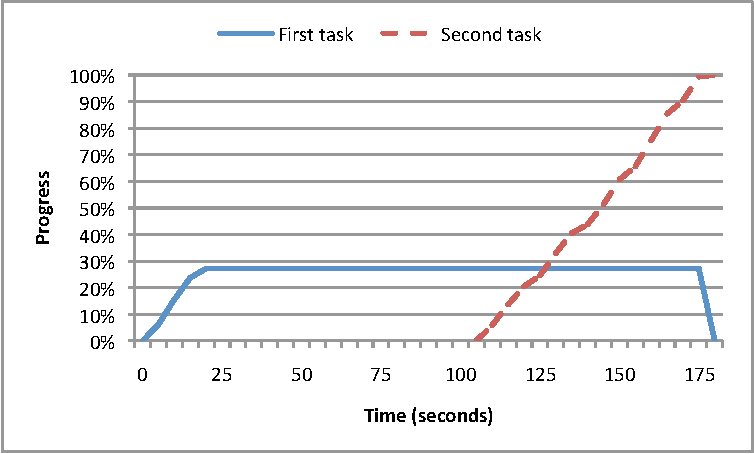
\includegraphics[width=0.48\linewidth]{figures/taskSpecPolicy_vanilla}}
  \subfloat[][HOP alert based task speculation policy]{\label{fig:spec-hop}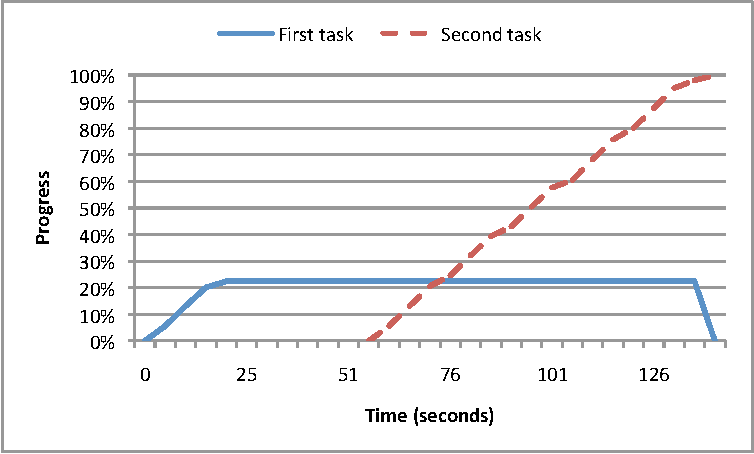
\includegraphics[width=0.48\linewidth]{figures/taskSpecPolicy_hop}}
  \caption{Compares speculation policies by plotting the starting point and progress of the faulty task (first task) and speculative task (second task).}
\label{fig:taskSpecPolicy}
\end{figure*}

We compared our alert based speculation policy with the speculation policy
implemented in unmodified Hadoop 19.2.  Our experiment executed a wordcount job
that contained a single faulty map task that would execute normally for a
minute before stalling out by sleeping for one second intervals between map
function invocations.  The input to the wordcount was 10GB of randomly
generated words, yielding 20 map tasks total.  We executed this job on a 20
node EC2 cluster and compared the time it took to initiate a speculative task
using our policy to the policy in unmodified Hadoop.

Figure~\ref{fig:taskSpecPolicy} shows the result of this experiment by plotting
the launch time and progress of the original (first) task and the backup
(second) task.  HOP's alert based speculation policy is able to detect the
faulty map task and execute a backup task in half the time of unmodified
Hadoop.  In unmodified Hadoop, a task is speculated based on its rate of
progress (relative to other tasks in its category).  We are able to further
extend this policy by including machine and process level statistics as further
evidence to speculate.  Indeed, our choice to speculate was not only based on a
high estimated time to completion but also a critically low ``user CPU'' value
and a critically low I/O activity.

The astute reader will notice however that the rate of progress for the second
task in HOP is less than that of unmodified Hadoop.  The reason for this is
that our monitoring jobs do add some extra load to the cluster.  Nevertheless,
in this instance, the overall job response time was slightly less (a few
seconds) in HOP due to the faster turn around time in our speculation policy.


\section{Related Work}
\label{ch:hop:sec:relwork}

This work relates to literature on parallel dataflow frameworks, online
aggregation, and continuous query processing.

\subsection{Parallel Dataflow}

Dean and Ghemawat's paper on Google's MapReduce~\cite{mapreduce-osdi} has
become a standard reference, and forms the basis of the open-source Hadoop
implementation.  The Google MapReduce design targets very large clusters where
the probability of worker failure or slowdown is high.  This led to their
elegant checkpoint/restart approach to fault-tolerance, and their lack of
pipelining.  Our work extends the Google design to accommodate pipelining
without significant modification to their core programming model or fault
tolerance mechanisms.

{\em Dryad}~\cite{dryad07} is a data-parallel programming model and runtime
that is often compared to MapReduce, supporting a more general model of acyclic
dataflow graphs.  Like MapReduce, Dryad puts disk materialization steps between
dataflow stages by default, breaking pipelines.  The Dryad paper describes
support for optionally ``encapsulating'' multiple asynchronous stages into a
single process so they can pipeline, but this requires a more complicated
programming interface.

It has been noted that parallel database systems have long provided partitioned
dataflow frameworks~\cite{pavlo09}, and recent commercial databases have begun
to offer MapReduce programming models on top of those
frameworks~\cite{aster,greenplum}.  Most parallel database systems can provide
pipelined execution akin to our work here, but they use a more tightly coupled
iterator and {\em Exchange} model that keeps producers and consumers
rate-matched via queues, spreading the work of each dataflow stage across all
nodes in the cluster~\cite{exchange}.  This provides less scheduling
flexibility than MapReduce and typically offers no tolerance to mid-query
worker faults.  Yang et al.\ recently proposed a scheme to add support for
mid-query fault-tolerance to traditional parallel databases, using a
middleware-based approach that shares some similarities with
MapReduce~\cite{osprey-icde}.

Logothetis and Yocum describe a MapReduce interface over a continuous query
system called {\em Mortar} that is similar in some ways to our
work~\cite{logoyocum08}.  Like HOP, their mappers push data to reducers in a
pipelined fashion.  They focus on specific issues in efficient stream query
processing, including minimization of work for aggregates in overlapping
windows via special reducer APIs.  They are not built on Hadoop, and explicitly
sidestep issues in fault-tolerance.

{\em Hadoop Streaming} is part of the Hadoop distribution, and allows map and
reduce functions to be expressed as UNIX shell command lines.  It does not
stream data through map and reduce phases in a pipelined fashion.

\subsection{Online Aggregation}

Online aggregation was originally proposed in the context of simple
single-table SQL queries involving ``Group By'' aggregations, a workload quite
similar to MapReduce~\cite{onlineagg}.  The focus of the initial work was on
providing not only ``early returns'' to these SQL queries, but also
statistically robust estimators and confidence interval metrics for the final
result based on random sampling.  These statistical matters do not generalize
to arbitrary MapReduce jobs, though our framework can support those that have
been developed.  Subsequently, online aggregation was extended to handle join
queries (via the {\em Ripple Join} method), and the {\em CONTROL} project
generalized the idea of online query processing to provide interactivity for
data cleaning, data mining, and data visualization tasks~\cite{ieeecontrol}.
That work was targeted at single-processor systems.  Luo et al.\ developed a
partitioned-parallel variant of Ripple Join, without statistical guarantees on
approximate answers~\cite{luo-ripple}.

In recent years, this topic has seen renewed interest, starting with Jermaine
et al.'s work on the {\em DBO} system~\cite{dbo}.  That effort includes more
disk-conscious online join algorithms, as well as techniques for maintaining
randomly-shuffled files to remove any potential for statistical bias in
scans~\cite{jermaine-shuffle}.  Wu et al.\ describe a system for peer-to-peer
online aggregation in a distributed hash table context~\cite{wu-vldb09}.  The
open programmability and fault-tolerance of MapReduce are not addressed
significantly in prior work on online aggregation.

An alternative to online aggregation combines precomputation with sampling,
storing fixed samples and summaries to provide small storage footprints and
interactive performance~\cite{gibbons98new}.  An advantage of these techniques
is that they are compatible with both pipelining and blocking models of
MapReduce.  The downside of these techniques is that they do not allow users to
choose the query stopping points or time/accuracy trade-offs
dynamically~\cite{ieeecontrol}.

\subsection{Continuous Queries}

In the last decade there was a great deal of work in the database research
community on the topic of continuous queries over data streams, including
systems such as Borealis~\cite{borealis}, STREAM~\cite{stream}, and
Telegraph~\cite{tcq-cidr}.  Of these, Borealis and Telegraph~\cite{flux-ft}
studied fault-tolerance and load balancing across machines.  In the Borealis
context this was done for pipelined dataflows, but without partitioned
parallelism: each stage (``operator'') of the pipeline runs serially on a
different machine in the wide area, and fault-tolerance deals with failures of
entire operators~\cite{borealisFT}.  SBON~\cite{sbon} is an overlay network
that can be integrated with Borealis, which handles ``operator placement''
optimizations for these wide-area pipelined dataflows.

Telegraph's {\em FLuX} operator~\cite{flux-ft,flux-lb} is the only work to our
knowledge that addresses mid-stream fault-tolerance for dataflows that are both
pipelined and partitioned in the style of HOP\@.  FLuX (``Fault-tolerant,
Load-balanced eXchange'') is a dataflow operator that encapsulates the
shuffling done between stages such as map and reduce.  It provides
load-balancing interfaces that can migrate operator state (e.g., reducer state)
between nodes, while handling scheduling policy and changes to data-routing
policies~\cite{flux-lb}.  For fault-tolerance, FLuX develops a solution based
on process pairs~\cite{flux-ft}, which work redundantly to ensure that operator
state is always being maintained live on multiple nodes.  This removes any
burden on the continuous query programmer of the sort we describe in
Chapter~\ref{ch:hop:sec:continuous}.  On the other hand, the FLuX protocol is
far more complex and resource-intensive than our pipelined adaptation of
Google's checkpoint/restart tolerance model.

\section{Summary}

In this chapter, we extended the batch-oriented execution model of MapReduce to
support pipelining between operators.  This enables a new suite of MapReduce
jobs that are able to perform online aggregation and continuous like queries.
Unlike much of the work on online aggregation, we do not focus here on
statistical guarantees because of the flexibility of the MapReduce programming
model.  These guarantees are crafted for specific SQL aggregates like SUMs,
COUNTs, and AVERAGEs, and modified to account for processing techniques like
the join algorithms used.  The focus of our work here is architectural: to
provide ``early returns'' interactions within the powerful scalability and
fault-tolerance facilities of MapReduce frameworks.  The statistical guarantees
from the literature only apply to SQL-style reduce functions; statistical
guarantees for other online reducers would need to be developed in a
case-by-case basis.  We expect that in many cases users will settle for simply
observing changes in the output of a job over time, and make their own
decisions about whether early returns are sufficient.

We leveraged our ability to run continuous MapReduce jobs in HOP by developing
a monitoring framework that provides near real-time machine and process level
statistics.  Our monitoring framework enabled new scheduling opportunities that
are based on such statistics.  Porting the declarative scheduler to HOP allowed
us to quickly prototype alternative policies in \OVERLOG where, in many cases,
adding new scheduling constraints translated into adding/removing a few rule
predicates.





\chapter[Conclusion and Future Extensions]{Conclusion and Future Extensions}
\label{ch:conclusion}

MapReduce has proven to be a popular model for large-scale parallel programming. Our Hadoop Online Prototype extends the applicability of the model to pipelining behaviors, while preserving the simple programming model and fault tolerance of a full-featured MapReduce framework.  This provides significant new functionality, including ``early returns'' on long-running jobs via online aggregation, and continuous queries over streaming data.  We also demonstrate benefits for batch processing:  by pipelining both within and across jobs, HOP can 
%achieve increased parallelism, improved system utilization, and 
reduce the time to job completion. 

In considering future work, scheduling is a topic that arises immediately.
Stock Hadoop already has many degrees of freedom in scheduling batch tasks across machines and time, and the introduction of pipelining in HOP only increases this design space.  First, pipeline parallelism is a new option for improving performance of MapReduce jobs, but needs to be integrated intelligently with both intra-task partition parallelism and speculative redundant execution for ``straggler'' handling.
%But given a fixed budget of task slots the cluster can run, pipeline depth has to be traded off against the number of concurrent partitions of a single dataflow stage (a single map or reduce).  We hope to expose these tradeoffs better via a closer analysis of the burstiness of resource consumption in stock Hadoop, and the resulting opportunity to smooth those bursts with pipelined parallelism.  
Second, the ability to schedule deep pipelines with direct
communication between reduces and maps (bypassing the distributed file
system) opens up new opportunities and challenges in carefully co-locating tasks from different jobs, to avoid communication when possible.  
%Finally, pipelining has tradeoffs with the use of map-side combiners.  As noted in Section~\ref{ch:hop:sec:pipelining}, for jobs that generate a small number of distinct reduce keys (e.g., genders), eager pipelining defeats the data reduction opportunities available with a blocking map-side combiner. For jobs with many reduce keys, or with no combiner available (e.g. Sort), aggressive pipelining may be a wise choice, to enable pipelined parallelism.  Since the number of distinct reduce keys is not typically known in advance, the choice of batch sizes for pipelining should be chosen in a dynamic fashion based on introspection during processing.  This introspection could be node-local, or could be a global decision fed by a continuous monitoring query of the sort illustrated in Section~\ref{ch:hop:sec:continuous}.  

Olston and colleagues have noted that MapReduce systems---unlike traditional databases---employ ``model-light'' optimization approaches that gather and react to performance information during runtime~\cite{olston-usenix08}.  The continuous query facilities of HOP enable powerful introspective programming interfaces for this: a full-featured MapReduce interface can be used to script performance monitoring tasks that gather system-wide information in near-real-time, enabling tight feedback loops for scheduling and dataflow optimization.  This is a topic we plan to explore further, including opportunistic methods to do monitoring work with minimal interference to outstanding jobs, as well as dynamic approaches to continuous optimization in the spirit of earlier work like Eddies~\cite{eddies} and FLuX~\cite{flux-lb}.

% Inter-job pipelining brings up some interesting opportunities for optimization as well. First, if we have a chain of two jobs, we can have the
% first job write its output to the local disk instead of going to HDFS. This
% saves the HDFS overhead at the expense of the risk of local disk failure.
% Since the intermediate data is relatively ephemeral, the window of risk may be tolerable in many cases. Second, we want to try scheduling maps of second job at nodes where reduces of the first job are running. This way data pipelining will be done locally and will not have to go through the network.

% Online aggregation changes some of the scheduling criteria in cases where there are not enough slots systemwide for all of a job's tasks.  Map and reduce tasks affect an online aggregation job differently: leaving map tasks unscheduled is akin to sampling the input file, whereas leaving reduce tasks unscheduled is akin to missing certain output keys -- some of which could be from groups with many inputs.  This favors reducers over mappers, at least during early stages of processing.  

% In order to improve early results of pipelined flows (e.g., for online aggregation), it is often desirable to prioritize ``interesting'' data in the pipeline, both at the mapper and reducer.  Online reordering of data streams has been studied in the centralized setting~\cite{juggle}, but it is unclear how to expose it in the MapReduce programming framework, with multiple nodes running in parallel -- especially if the data in the input file is not well randomized.  

%Continuous queries over streams raise many specific opportunities for optimizations, including sharing of work across queries on the same streams, and minimizing the work done per query depending on windowing and aggregate function semantics.  Many of these issues were previously considered for tightly controlled declarative languages on single machines~\cite{stream,tcq-cidr}, or for wide-area pipelined dataflows~\cite{borealis,sbon}, and would need to be rethought in the context of a programmable MapReduce framework for clusters.
 % many of which have been well-studied in the literature and should port naturally to a MapReduce setting, as demonstrated in initial work on the topic~\cite{logoyocum08}.  One key issue in the literature is the sharing of work across multiple queries on the same stream~\cite{precisionsharing,huebsch}; but prior work does not necessarily map well to a MapReduce framework, and the issue deserves more investigation.  
%Introspective system monitoring is a good driving application here, since it provides a well-motivated workload that developers of the system are well-motivated to study in depth.  

As a more long-term agenda, we want to explore using MapReduce-style programming for even more interactive applications.  As a first step, we hope to revisit interactive data processing in the spirit of the CONTROL work~\cite{ieeecontrol}, with an eye toward improved scalability via parallelism.  More aggressively, we are considering the idea of bridging the gap between MapReduce dataflow programming and lightweight event-flow programming models like SEDA~\cite{seda}.  Our HOP implementation's roots in Hadoop make it unlikely to compete with something like SEDA in terms of raw performance. However, it would be interesting to translate ideas across these two traditionally separate programming models, perhaps with an eye toward building a new and more general-purpose framework for programming in architectures like cloud computing and many-core.



% ===============================
% Part III: Back Matters
%           - bibliography
%           - appendix
%           - index
% ===============================

%\ssp
\nocite{*}
\bibliographystyle{plain}
\bibliography{thesis}

\end{document}


\end{document}
